\documentclass[a4paper, 11pt]{memoir}
\RequirePackage{fullpage}
\RequirePackage[pass]{geometry}
\RequirePackage{hyperref}
\RequirePackage{mathtools}
%\RequirePackage{float}
  \setcounter{secnumdepth}{2} % seting level of numbering (default for "report" is 3). With ''-1'' you have non number also for chapters
  \setcounter{tocdepth}{2} % if you want all the levels in your table of contents
\RequirePackage{todonotes}
%\RequirePackage[disable]{todonotes}
  \let\Oldtodo\todo
  \renewcommand{\todo}[1]{\Oldtodo[inline]{#1}}
\RequirePackage{graphicx} % for images
  \graphicspath{{./figures/}}
\RequirePackage{subcaption}
\RequirePackage[binary-units=true]{siunitx}
  \sisetup{per-mode=symbol} % to print GB/s instead of GBs^(-1)
\RequirePackage{multirow}
%\RequirePackage{floatrow} % for subfigure vertical alignment.

  \newsavebox{\tempbox} % for aligning subfigures

  % parskip package does not work for memoir class
  \nonzeroparskip
  \setlength{\parindent}{0pt}
\RequirePackage[]{hyphenat} %\nohyphenation

\RequirePackage[hang]{footmisc} % for multiline footnote alignment
  \setlength\footnotemargin{10pt}

% since im not using the IEEEtran document style, this is needed to get \bstctlcite{} to work.
% https://tex.stackexchange.com/questions/16506/bibliography-author-initial-spacing
  \makeatletter
  \def\bstctlcite{\@ifnextchar[{\@bstctlcite}{\@bstctlcite[@auxout]}}
  \def\@bstctlcite[#1]#2{\@bsphack
    \@for\@citeb:=#2\do{%
      \edef\@citeb{\expandafter\@firstofone\@citeb}%
      \if@filesw\immediate\write\csname #1\endcsname{\string\citation{\@citeb}}\fi}%
    \@esphack}
  \makeatother

\usepackage{mathpazo}
%\usepackage[sc,osf]{mathpazo}
%\RequirePackage{fontspec}
  %\setmonofont{Menlo-Regular.ttf}[Scale=MatchLowercase]

% Listing and specifics for Verilog highlighting.
% Highlight-to-color source: https://github.com/atom/one-dark-syntax/blob/master/styles/syntax-variables.less
% Color-to-HSL source: https://github.com/atom/one-dark-syntax/blob/master/styles/colors.less
% HSL-to-RGB source: https://www.rapidtables.com/convert/color/hsl-to-rgb.html
\usepackage{listings}
% From DARK theme.
%\definecolor{hue-3}{RGB}{198,120,221} %purple
%\definecolor{hue-6}{RGB}{209,154,102} %orange
%\definecolor{hue-6-2}{RGB}{229,192,123} %orange
%\definecolor{bg}{RGB}{40,44,52} %background
%\definecolor{fg}{RGB}{171,178,191} %text foreground

% From LIGHT theme
\definecolor{hue-1}{RGB}{1,132,188} %cyan
\definecolor{hue-3}{RGB}{166,38,164} %purple
\definecolor{hue-6}{RGB}{152,104,1} %orange 1
\definecolor{bg}{RGB}{250,250,250} %background
\definecolor{fg}{RGB}{56,58,66} %text foreground

\newcommand*{\FormatDigit}[1]{\textcolor{hue-6}{#1}}

\lstdefinestyle{verilog-style}
{
    language=Verilog,
    captionpos=b, % caption at bottom
  %  backgroundcolor = \color{bg},
    basicstyle=\small\ttfamily\color{fg},
    keywordstyle=\color{hue-3},
    keywordsprefix=\$,alsoletter=\$,
    identifierstyle=\color{fg},
    commentstyle=\color{green},
    numbers=left,
    numberstyle=\tiny\color{black}\ttfamily, % line number style
    numbersep=10pt,
    tabsize=2,
    frame=single, % frame around code
    rulecolor=\color{fg}, % color of frame TODO: depends on if LIGHT or DARK theme is used.
    keepspaces=true, % keeps spaces in text, useful for keeping indentation of code (possibly needs columns=flexible)
literate={0}{{\FormatDigit{0}}}{1}%
     {1}{{\FormatDigit{1}}}{1}%
     {2}{{\FormatDigit{2}}}{1}%
     {3}{{\FormatDigit{3}}}{1}%
     {4}{{\FormatDigit{4}}}{1}%
     {5}{{\FormatDigit{5}}}{1}%
     {6}{{\FormatDigit{6}}}{1}%
     {7}{{\FormatDigit{7}}}{1}%
     {8}{{\FormatDigit{8}}}{1}%
     {9}{{\FormatDigit{9}}}{1}%
     {.0}{{\FormatDigit{.0}}}{2}% Following is to ensure that only periods
     {.1}{{\FormatDigit{.1}}}{2}% followed by a digit are changed.
     {.2}{{\FormatDigit{.2}}}{2}%
     {.3}{{\FormatDigit{.3}}}{2}%
     {.4}{{\FormatDigit{.4}}}{2}%
     {.5}{{\FormatDigit{.5}}}{2}%
     {.6}{{\FormatDigit{.6}}}{2}%
     {.7}{{\FormatDigit{.7}}}{2}%
     {.8}{{\FormatDigit{.8}}}{2}%
     {.9}{{\FormatDigit{.9}}}{2}%
     %{,}{{\FormatDigit{,}}{1}% depends if you want the "," in color
     {\ }{{ }}{1}% handle the space
}

% Source: https://tex.stackexchange.com/questions/42961/adding-a-highlight-to-texttt-blocks
\usepackage{xcolor}
\usepackage{soul}

\definecolor{Light}{gray}{.90}
\sethlcolor{Light}

\let\OldTexttt\texttt
\renewcommand{\texttt}[1]{\OldTexttt{\hl{#1}}}% will affect all \texttt
%\newcommand{\hltexttt}[1]{\texttt{\hl{#1}}}% comment above \renewcommand if want this



% https://tex.stackexchange.com/questions/23726/error-in-memoir-command-newfloat-already-defined
\let\newfloat\undefined
\usepackage{floatrow}
\usepackage{fancybox}
\captionsetup[subfigure]{labelformat=parens,labelsep=space}
%\floatsetup{style=plain,valign=c}
\DeclareColorBox{yellowplate}{\colorbox{white}} \floatsetup{style=plain,framestyle=colorbox,
        framearound=row,colorframeset=yellowplate,frameset={\fboxrule0pt},
        framestyle=colorbox,framefit=yes,heightadjust=object,valign=c}
\floatsetup[table]{style=plaintop}




\begin{document}
  \bstctlcite{IEEEexample:BSTcontrol} % needed for the control entry in the bib to work.
  
  \cleardoublepage
  \thispagestyle{empty}
\begin{titlingpage}
    \centering
    
\includegraphics{./frontmatter/images/TU_Delft_logo_Black.eps}\\
    {\LARGE Delft University of Technology}\\[1.2em]

    \textit{Electrical Engineering, Mathematics, and Computer Science} \\
    \textit{Computer Engineering} \\
    \vfill
    {\LARGE Feeding High-Bandwidth Streaming-Based FPGA Accelerators} \\
    \vfill
    \begin{flushright}
        {\large \textit{Thesis{} by:} \\[0.5em]
        Yvo Thomas Bernard Mulder\\[0.5em]
        }
    \end{flushright}
    \begin{flushleft}
        {\large \textit{Advisor}: \\[0.5em]
        Prof. Dr. H.P. Hofstee
        \\[1.5em]
        \textit{Committee:}\\[1em]
        \textit{Chair:} \\[0.2em]
        Prof. Dr. H.P. Hofstee \\[1em]
        \textit{Members:} \\[0.2em]
        Dr. Ir. Z. Al-Ars\\
        Dr. Ir. R. van Leuken\\}
    \end{flushleft}

\end{titlingpage}

  \cleardoublepage
  \thispagestyle{empty}
\begin{vplace}
    
\centering
{\LARGE Feeding High-Bandwidth Streaming-Based FPGA Accelerators}
\\[4em]
{\large
\textsc{Thesis} \\[1.5em]
submitted in partial fulfillment of the requirements for the degree of \\[1em]
\textsc{Master of Science}
\\[1em]
in
\\[1em]
\textsc{Computer Engineering}
\\[1em]
by
\\[1em]
\textsc{Yvo Thomas Bernard Mulder}\\[0.5em]
born in \textsc{Utrecht, The Netherlands}
\\[1em]
to be defended publicly on January 29, 2018 at 15:00.
}
\end{vplace}
\vfill
\begin{flushleft}
\noindent
CE-MS-2018-05\\
ISBN: 978-94-6186-886-2\\
Computer Engineering\\
Faculty of Electrical Engineering, Mathematics, and Computer Science\\
Delft University of Technology\\
Mekelweg 4,\\
2628 CD, Delft\\
The Netherlands \\
\end{flushleft}

  %\cleardoublepage
  %\include{chapters/0-thanks}

  %\begin{titlingpage}

\begin{center}



%% Insert the TU Delft logo at the bottom of the page.
%\begin{tikzpicture}[remember picture,overlay]
%    \node [inner sep=0pt] at (-5,-25)
%    {\includegraphics{cover/logo}};
%    \node [inner sep=0pt] at (5,-25)
%    {\includegraphics[width=.3\textwidth]{cover/EILlogo}};
%\end{tikzpicture}

%% Insert the TU Delft logo at the bottom of the page.
%\begin{tikzpicture}[remember picture,overlay]
%    \node at (current page.south)[anchor=south,inner sep=0pt]{
%        \includegraphics{cover/logo}
%    };
%\end{tikzpicture}

%% Extra whitespace at the top.
\vspace*{2\bigskipamount}

%% Print the title in cyan.
{\makeatletter
%\titlestyle
\color{black}\Huge Feeding High-Bandwidth Streaming-Based FPGA Accelerators
\makeatother}

%% Print the optional subtitle in black.
{\makeatletter
\ifx\@subtitle\undefined\else
    \bigskip
    %\titlefont
    \titleshape\LARGE MSc Thesis
\fi
\makeatother}

\bigskip
\bigskip

by
%door

\bigskip
\bigskip

%% Print the name of the author.
{\makeatletter
%\titlefont
\Large Yvo Thomas Bernard Mulder
\makeatother}

\vfill

in partial fulfillment of the requirements for the degree of
%in overeenstemming met de vereisten voor het verkrijgen van de graad van

\bigskip
\bigskip

MASTER OF SCIENCE

\bigskip

in

\bigskip

\textsc{COMPUTER ENGINEERING}

\bigskip
\bigskip

at the Delft University of Technology\\

to be defended publicly on January 29th, 2018 at 15:00.
%in het openbaar de verdedigen op dinsdag 1 januari om 10:00 uur.

\vfill

\begin{tabular}{lll}
%% Add additional information here, per faculty requirements, e.g
%    Student number: & 1234567 \\
%    Project duration: & \multicolumn{2}{l}{March 1, 2012 -- January 1, 2013} \\
    Supervisor: & Prof. dr. ir. H. P. Hofstee, CE, TU Delft\\
                \\
    Thesis committee:
        & Prof. dr. ir. H. P. Hofstee, CE, TU Delft\\
        & Associate prof. dr. ir. Z. Al-Ars, CE, TU Delft\\
        & Associate prof. dr. ir. R. van Leuken, CAS, TU Delft\\
\end{tabular}

%% Only include the following lines if confidentiality is applicable.
\bigskip
\bigskip
\emph{This thesis is confidential and cannot be made public until February 1, 2018.}
%\emph{Op dit verslag is geheimhouding van toepassing tot en met 31 december 2013.}

\bigskip
\bigskip
An electronic version of this thesis is available at \url{http://repository.tudelft.nl/}.
%Een elektronische versie van dit verslag is beschikbaar op \url{http://repository.tudelft.nl/}.

\end{center}

\end{titlingpage}


  \chapter*{Abstract}

A new class of accelerator interfaces has significant implications on system architecture. An order of magnitude more bandwidth forces us to reconsider FPGA design. OpenCAPI is a new interconnect standard that enables attaching FPGAs coherently to a high-bandwidth, low-latency interface. Keeping up with this bandwidth poses new challenges for the design of accelerators, and the logic feeding them.

This thesis is conducted as part of a group project, where three other master students investigate database operator accelerators. This thesis focuses on the logic to feed the accelerators, by designing a reconfigurable multi-stream buffer architecture. By generalizing across multiple common streaming-like accelerator access patterns, an interface consisting of multiple read ports with a smaller than cache line granularity is desired. At the same time, multiple read ports are allowed to request any stream, including reading across a cache line boundary.

The proposed architecture exploits different memory primitives available on the latest generation of Xilinx FPGAs. By combining a traditional multi-read port approach for data duplication with a second level of buffering, a hierarchy typically found in caches, an architecture is proposed which can supply data from 64 streams to eight read ports without any access pattern restrictions.

A correct-by-construction design methodology was used to simplify the validation of the design and to speedup the implementation phase. At the same time, the design methodology is documented and examples are provided for ease of adoption. With the design methodology, the proposed architecture has been implemented and is accompanied by a validation framework.

Various configurations of the multi-stream buffer have been tested. Configurations up to 64 streams with four read ports meet timing with an AFU request-to-response latency of five cycles. The largest configuration with 64 streams and eight read ports fails timing. Limiting factors are the inherent architecture of FPGAs, where memories are physically located in specific columns. This makes extracting data complex, especially at the target frequencies of \SI{200}{\mega\hertz} and \SI{400}{\mega\hertz}. Wires are scattered across the FPGA and wire delay becomes dominant.

FPGA design at increasing bandwidths requires new design approaches. Synthesis results are no guarantee for the implemented design, and depending on the design size, could indicate a very optimistic operating frequency. Therefore, designing accelerators to keep up with an order of magnitude more bandwidth compared to the current state-of-the-art is complex, and requires carefully thought out accelerator cores, combined with an interface capable of feeding it.



%CPU performance is reaching a plateau, which pushes the adoption of heterogeneous system architectures. Attaching compute resources such as GPUs and FPGAs, but also network and storage, requires an increase in IO bandwidth. The implications of such a change on FPGA design are of interest, in particular in conjunction with the OpenCAPI interconnect standard.\\


%\todo{IBM BOE talk questions:\\
%- use these slides as inspiration as well.\\
%- why not use a cache instead of your buffer? Would a cache benefit? For example, if it was already present?\\
%- How about security? Enterprise requires high security (Wolfgang Maier). A solution could be to place an encryption engine before the actual AFU.\\
%- if we would change system architecture and go to emerging memory technologies, how would this impact your module/design? (wolfgang)\\
%}

%Hercules and the Hydra as front cover. Hercules represents a lone engineer, confronted with a multi-facetted problem. But the multiple heads also represent the multiple read ports of the buffer, which have to be fed with data.\\
%Read the actual myth and see if I can link the story more to the thesis. \url{https://en.wikipedia.org/wiki/Lernaean_Hydra}


%\todo{Thesis outline according to Peter @ 17th July (keep it for future reference)\\
%Intro\\
%- Technology trends -> accelerators -> cost of accelerator versus cost of feeding it data (very important!)\\
%- interconnect trends, bandwidth, coherence/memory sharing\\
%- aim of the thesis / contributions\\

%Ch 1\\
%- Accelerator types (classification according to memory access)\\
%- Streaming accelerators (not trivial, show sorter as an example)\\
%-- sorter example: streaming is difficult with more and more streams. also reading across cache line boundary is difficult.\\
%-- why does naive implementation not work?\\
%- OpenCAPI/FPGA characteristics (maybe in chapter 2)\\

%Ch 2\\
%- Specification / Implementation (design choices \& Andy's design methodology)\\

%Ch 3\\
%Variations and Generalizations (read-only caches) / analysis\\
%For examples of variations, see picture I took of the white board.\\
%A variation could be to have 32 streams instead of 64 but each stream (both in L1 and L2) can buffer twice as much cache lines. Might %be interesting when the AFU hits one stream at a time.\\
%For the analysis part here; maybe a trace is interesting but more interested in principles. Use formulas.\\

%5Ch Conclusions etc\\

%Other notes from meeting:\\
%- Repeating throughout the thesis should be: streaming, spatial/temporal locality, random access.\\
%- Cost of FPGAs is not in functional unit but in getting data there.\\
%- Talk about granularity both on the OpenCAPI and AFU rd port side.\\
%- streaming is an extreme case of spatial locality\\
%- granularity was much harder than one might expect in this thesis.\\
%- If you would ignore the granularity, then you would have a 128B cache line at the AFU. What will you do with that? Smaller %granularity is needed.\\
%- Check presentations folder on Google Drive as well.\\
%}

  \cleardoublepage

  \chapter*{Preface}

This thesis report marks the end of this project, on which I have worked for a year. The year started at the IBM Austin Research Lab, after Peter Hofstee invited me to work with him on emerging coherently attached FPGA accelerators. During my six months in Austin, Peter was always ready to help and chat. Also in the period after Austin was Peter always available. Peter, it has been a very pleasant journey and I sincerely hope our paths cross again. I can safely say that you not only have been a tremendous supervisor, but also a good friend.

Because the project is in the field of FPGAs, I had many interesting discussions with Andrew Martin. Andrew is a research staff member and developed a ready-valid design methodology for FPGA design. Andy, I would like to thank you for your support during the design and implementation phase. Your methodology is the missing link for FPGA design.

Dorus, Eric, Jeremy, and Jinho, the three o'clock stretch session must live on, but in different countries and time zones. I enjoyed my time in Austin very much and that is thanks to you.

I would like to thank the Universiteitsfonds for providing funding for the six months I spent in Austin. Without this support, it would have been difficult to have had this experience.

I would like to thank my parents for their life-long support and faith in me.

Finally, I would like to thank Fjóla for always being there for me when I needed her the most and making me a better person every day.

  \cleardoublepage

  \tableofcontents* % The '*' removes the self-reference of 'Contents'.
  \newpage
  \listoffigures
  \newpage
  \listoftables
  \lstlistoflistings

  \chapter*{Revision Log}
  \addcontentsline{toc}{chapter}{Revision Log}
  The revision log keeps track of all significant changes that have been made to this thesis since the initial public release on the 29th of January 2018. The most recent version of this document can be found at \url{https://github.com/ytbmulder/msc-thesis}.

  \begin{table}[H]
    \centering
    \begin{tabular}{ p{1.5cm} | p{3.5cm} | p{9.6cm} }
      \textbf{Version} & \textbf{Revision Date} & \textbf{Description} \\ \hline
      v1.0.0 & 29 January 2018 & Initial public release. \\
      v1.0.1 & 26 April 2018   & Addition of this revision log. \\
    \end{tabular}
  \end{table}

  \chapter{Introduction}
\label{sec:intro}

In recent years, data centers have been forced to embrace heterogeneous system architectures. As microprocessor technology and design is not able to deliver cost per performance improvements in line with historical rates, deployment of hardware acceleration will become commonplace.

% - increase in bandwidth changes design methodologies / approaches.
Trends in system architecture show that interconnect bandwidth is significantly increasing in order to provide data centers with the connectivity and ability to attach accelerators for any workload. Traditionally FPGAs (Field Programmable Gate Arrays) lacked bandwidth and programmability and could only be used for the most computationally intensive tasks, but recent advancements target these shortcomings and accelerate adoption. While the change in programming models is an interesting field of study, this thesis focuses on the emerging FPGAs with main memory class bandwidth enabled by such advancements. This change requires re-evaluation of our current design approaches and methodologies for accelerators. It does not only pose a challenge for accelerator design, but also for providing them with data. New interface logic is required to feed the accelerators, and new accelerator cores are needed, at least in those cases where the problem is not trivially parallel.

%Hardware accelerators are located inside the CPU package or attached externally and include ASICs, FPGAs and (GP)GPUs. Each type of accelerator excels at a specific type of workload in terms of flexibility and power efficiency. The most commonly used accelerator is the GPGPU, since it is applicable to a wide range of workloads such as analytics, computational science and machine learning. However, not all types of workloads map efficiently on a CPU or GPU. Therefore, ASICs and FPGAs are gaining popularity for certain workloads due to the order of magnitude increase in energy efficiency compared to CPUs and GPUs. Mostly compute-intensive workloads are suitable since the desired algorithm can be implemented as a fixed set of transformations on the input data. On the contrary, memory-intensive workloads suffer from a two-fold interconnect bottleneck between the CPU and attached accelerator. On one hand, the bandwidth is an order of magnitude less compared to system memory. On the other hand, accelerators are difficult to program due to the separate address space and are forced to copy through main memory. Finally, driver overhead increases latency.\\
%However, recent advancements in interconnect standards and the increase in bandwidth that comes with it enables these accelerators to be used for memory-intensive workloads as well and improves programmability significantly by providing a shared address space which makes accelerators act as peers to other processor cores. These advancements are essential in the data center of tomorrow.

% - Why streaming / multi-stream?
A common memory access pattern for FPGA accelerators is streaming and examples include content delivery, cryptography and databases. An interface capable of handling multiple streams is desired because workloads exist that inherently use multiple streams or for which multiple single-stream engines are required to work in parallel in order to exploit all of the available bandwidth. Besides that, sustaining throughput is more difficult when using a single stream. Multiple streams can more easily keep the interconnect fully utilized since concurrent requests can be made. Partitioning the compute is left to the accelerator designer.

% - Previous work will not suffice.
Previous work such as the Streaming Framework \cite{brobbel-github, brobbel-slides} and SNAP (Storage, Networking, and Analytics Programming) Framework \cite{snap-github, snap-slides} for CAPI (Coherent Accelerator Processor Interface) 1.0 will not suffice, since these frameworks are not capable of handling this class of bandwidth, nor the number of streams. The frameworks target a bandwidth that is an order of magnitude smaller compared to OpenCAPI. SNAP also uses the coherent cache present in CAPI 1.0, but not present in OpenCAPI. Therefore a direct port is not trivial.

%\todo{
%- Add that previous work uses cache line granularity data interface (Brobbel 128B, SNAP 250MHz 512b AXI). This might be too large for certain workloads.
%}




\newpage
\section{Thesis Aim}
\label{sec:aim}
To combine both efforts of re-evaluating the interface and accelerator engine design, this thesis is part of a larger project, in collaboration with three other master students \cite{huang-msc-thesis, yang-msc-thesis, zeng-msc-thesis}, that focuses on accelerator core design. A harmonized effort is made by studying a re-emerging and inherently multi-stream workload: database operators. Preliminary findings have been presented at the H\textsuperscript{2}RC 2017 workshop \cite{h2rc}.

Database systems have been looking for architectures that achieve a high bandwidth to access the required data. FPGA acceleration was used in the past, but a recent trend is the usage of in-memory databases. In such systems, the database is located in host memory instead of on flash or mechanical storage. Now that interfaces like OpenCAPI are approaching host memory-like bandwidths and have coherent memory access, accelerating database operators using FPGAs by means of low latency memory access becomes relevant again.

The three other master students are also under supervision of Prof. Dr. H. Peter Hofstee. They will study three different multi-stream accelerators for database operators. The studied operators are: Decompress-Filter, Merge-Sort and Hash-Join.
%Each student will study one of the following database operators.
%\begin{itemize}
%  \item{\textbf{Decompress-filter} decompress incoming data and apply a filter to ideally obtain less data than was provided.}
%  \item{\textbf{Merge-sort} merge multiple pre-sorted streams of data and provide one sorted output stream.}
%  \item{\textbf{Hash-join} x.}
%\end{itemize}

The aim of this thesis is to study the implications of emerging high-bandwidth interconnects for FPGA accelerators, but more importantly their interface. Feeding accelerators with data and keeping up with the increased bandwidth is challenging. Prerequisite are multiple streams and read ports with less than cache line granularity. Providing such an interface is not trivial at this bandwidth. Therefore, the focus is on getting the data to the FPGA. Writing results back to the host is left as future work.





\section{Thesis Contributions}
The aims are to generalize across several common FPGA memory access patterns and to design and implement an interface that can be generally applicable to current and future high-bandwidth interconnects. Supplying a general interface to the FPGA designer will improve adoption and accelerate the design cycle. The contributions made in this thesis can be summarized as follows.
\begin{itemize}
  \item{A study of a new class of accelerator interfaces, and a more detailed overview of OpenCAPI (the first of its kind).}
  \item{Re-evaluation of design methodologies for high-bandwidth attached FPGAs.}
  \item{Provide documentation and examples for a delay-insensitive design methodology provided by Andrew K. Martin.}
  \item{A multi-level buffer architecture proposal and implementation, aware of fixed-size memory resources found on FPGAs, by exploiting features of different memory primitives and state-of-the-art memory resources.}
  \item{Improve adoption of high-bandwidth interconnect, with a special interest in OpenCAPI, attached streaming-based accelerators by providing a generalized and reconfigurable interface. This interface supports multiple streams and access patterns in order to be widely used while keeping up with the bandwidth.}
\end{itemize}





\section{Thesis Organization}
Chapter 2 describes technology trends with respect to system level bandwidth requirements and interconnect standards. Chapter 3 takes a brief look at the state-of-the-art interconnect standards and what sets them apart. Chapter 4 characterizes OpenCAPI, the POWER9 processor and future OpenCAPI-compatible Xilinx FPGAs. Chapter 5 takes a look at common accelerator memory access patterns and shows naive buffer designs for full-utilization of the available interconnect bandwidth. Chapter 6 introduces the \textit{Delay Insensitive Cell Library} which accelerates FPGA design by providing cells with a built-in ready-valid protocol. Chapter 7 combines the previous chapters and motivates the design choices made for a multi-stream buffer and highlights the essential modules of the design. Chapter 8 shows the validation setup, performance, and implementation results, and Chapter 9 concludes the thesis.
%presents variations and generalizations based on the final design and Chapter 10 concludes the thesis.

  \chapter{Technology Trends}
\label{ch:trends}
Data center workloads have increased and diversified over the last decade. These changes are driven by emerging workloads such as artificial intelligence, big data and machine learning, but also by an increased demand of cloud services and a shift of compute from the edge of the network to the data center due to an increase in mobile devices. The following itemization summarizes different classes of workloads and examples \cite{stuecheli-power9, amd-epyc-datasheet, gupta-xeon}.

\begin{itemize}
  \item{Analytics: Big Data, High-Frequency Trading, and In-Memory Database.}
  \item{Cloud: Search, Virtualization, and Web Servers.}
  \item{Communication: Packet Processing and Virtual Switching.}
  \item{High Performance Computing: Artificial Intelligence, Genomics and Machine Learning.}
  \item{Security: Encryption and Decryption.}
  \item{Storage: Compression and Deduplication.}
\end{itemize}

%- “[Meanwhile], P. K. Gupta, the general manager of Xeon+FPGA products in Intel’s data center group, said FPGAs can increase the performance of applications such as machine learning, cloud radio-access networks, edge computing and content delivery. Accelerators can [also] increase performance at lower total cost of ownership for targeted workloads.”\\
%\url{https://www.rambus.com/blogs/the-role-of-fpga-acceleration-in-the-data-center-and-beyond-2/}\\

These changes in data center workloads demand not only more and faster resources (such as cooling, network and servers), but also a diversification of compute resources that can be dynamically tailored to the workload in question. Traditionally, servers consist of a fixed set of resources such as compute, memory, storage and I/O and are aggregated into a pool. Workloads are then scheduled on one or multiple pools. This architecture frequently results in under-utilization of resources due to a drastic real-time adjustment in available resources for specific workloads. This results in reduced power efficiency, or performance per Watt \cite{rambus}. The most important metric when building a new data center is the Total Cost of Ownership (TCO): the cost of purchasing and installing the hardware plus the cost to operate and maintain the data center over time. The electricity costs are roughly 15\% of the TCO \cite{research-cloud} and power consumption is becoming one of the most import metrics for data center operation and future hardware investments. Systems have to offer performance and power efficiency, while in the past performance was the dominant driver behind new investments. This makes Application Specific Integrated Circuits (ASICs), FPGAs and Graphics Processing Units (GPUs) more and more interesting due to their performance-to-Watt ratio.
%With reduced power efficiency, the data center operator pays for electricity to keep the server idle instead of doing useful work.

%OPTIMIZING DATA-CENTER TCO WITH SCALE-OUT PROCESSORS
%https://infoscience.epfl.ch/record/181904/files/tco_ieeemicro12.pdf

%A Simple Model for Determining True Total Cost of Ownership for Data Centers
%http://www.missioncriticalmagazine.com/ext/resources/MC/Home/Files/PDFs/(TUI3011B)SimpleModelDetermingTrueTCO.pdf





\section{Acceleration in the Data Center}
Traditionally, Moore's Law (which predicted exponential growth in the number of transistors on a chip) correlated well with single processor performance due to the increase in operating frequency that accompanied device scaling. The increase in the number of transistors per chip at a constant cost means that transistors become smaller and, if all dimensions are scaled, are able to switch at higher speeds. This explains the constant increase in frequency of processors until roughly 2006.





\subsection{Dennard Scaling}
In 1974, Dennard observed that the necessary current and voltage scale with transistor shrinking. This observation is known as Dennard scaling. Therefore, power consumption is proportional to transistor area. The total power consumed is the sum of dynamic and static power. Dynamic power is consumed by charging capacitors in the circuit and is shown in \autoref{eq:power}. Static power is consumed when the circuit is in quiescence.

\begin{equation}
  P = \alpha \times C \times F \times V^2, \text{where}
  \label{eq:power}
\end{equation}

\begin{itemize}
  \item{\textit{P} is the dynamic power,}
  \item{$\alpha$ is the percentage of time the circuit switches,}
  \item{\textit{C} is the sum of gate and wiring capacitance,}
  \item{\textit{F} is the frequency at which the circuit operates, and}
  \item{\textit{V} is the operating voltage of the circuit.}
\end{itemize}

% Original text talking about threshold voltage instead of gate oxide scaling.
% By shrinking transistors, capacitance and voltage can be reduced resulting in a higher operating frequency for the same dynamic power consumption. However, Dennard ignored two transistor parameters which define a baseline power consumption for a transistor: leakage current and threshold voltage. Leakage current is a phenomenon where charge carriers sip through the insulating region of a transistor, even in a rest state. Leakage current increases exponentially as the insulator thickness decreases, which occurs with the aggressive scaling of transistors. The voltage threshold is the minimum voltage required to establish a conducting path. With shrinking transistors, power density increased. Insufficient cooling capacity resulted in hitting the so-called \textit{Power Wall} in 2006 and limits processor frequency to around \SI{4}{\giga\hertz} \cite{dennard-scaling}.

However, \autoref{eq:power} involves simplified assumptions, because in the 1970's sub-threshold leakage was playing a relatively small role with respect to total power consumption. After several decades, sub-threshold leakage constrains further scaling of the threshold voltage and therefore also operating voltage. Due to leakage constraints, gate oxide scaling has also been affected. This prevents voltages from scaling as in the past, and thus starts to play a significant part in the total chip power. These factors limit the operating frequency of circuits \cite{mark-bohr}. Because voltages no longer scale, shrinking transistors now leads to power density increases. Insufficient cooling capacity resulted in hitting the so-called \textit{Power Wall} in 2006 that limits processor frequency to around \SI{4}{\giga\hertz} \cite{dennard-scaling}.

% From "A 30 Year Retrospective on Dennard's MOSFET Scaling Paper" by Mark Bohr from Intel.
% - But this 1974 work ignored the impact of transistor sub-threshold leakage on overall chip power. Sub-threshold leakage was relatively low in the 1970’s and was a tiny contributor to total power consumption on logic circuits. But after 30 years of scaling, VT has scaled to the point where sub-threshold leakage has increased from levels of <10-10 amps/mm to >10-7 amps/mm. Due to leakage constraints, it will be difficult to further scale VT and thus it will also be difficult to scale operating voltage.
% - Another key assumption in Dennard’s scaling law was the ability to scale gate oxide thickness. Gate oxide scaling has been a key contributor to scaling improvements over the past 30 years, but this trend is also slowing due to leakage constraints (see Figure 4). Intel’s 65nm generation transistors use a SiO2 gate dielectric with a thickness of 1.2 nm [2]. This dielectric is only about 5 silicon atomic layers thick and represents what is likely the limit to which SiO2 can be scaled. Not only are we running out of atoms, but gate oxide leakage due to direct tunneling current is becoming a noticeable percentage of overall chip power.





\subsection{Homogeneous Multi-Core Systems}
%In order to comply with performance and power efficiency requirements, workloads have to be mapped onto a compute resource which fits both requirements best. In a hierarchy of compute resources based on power efficiency, defined as performance per Watt, a CPU is on one side of the spectrum and an ASIC on the other. A GPGPU and FPGA fit in between these extremes respectively. In such a hierarchy, there is an inverse relationship between power efficiency and workload versatility.
%A CPU is the most versatile but has the worst power efficiency for certain workloads, while the function of an ASIC is fixed but is highly optimized for a specific task, therefore achieving better power efficiency. With such a diversity of workloads, it is obvious that not all workloads map entirely efficient to only a CPU or GPU. Some classes might have fine-grained parts which map efficiently to one, while the rest maps efficiently to another, or any other possible combination. Then there are also classes, or parts thereof, which map to neither.\\

Since 2006, after hitting the \textit{Power Wall}, and well before 2006 for server processors, Central Processing Units (CPUs) started to have multiple cores that work in parallel. Cores can be located within the same package, across multiple sockets, or across multiple systems. However, a workload across multiple homogeneous cores scales only as well as the portion of the workload that can be parallelized. Amdahl's Law \cite{amdahl}, shown in \autoref{eq:amdahl}, formulates the theoretical speedup of a workload when a portion of the system is improved and encapsulates this notion. The speedup is limited by the fraction of the task that does not benefit from the improvement. For example, if a task consists of one portion that can be parallelized and one portion that cannot, eventually the total latency is always bounded by the purely sequential portion.

\begin{equation}
  S_{latency}(s) = \frac{1}{(1-p) + \frac{p}{s}}, \text{where}
  \label{eq:amdahl}
\end{equation}

\begin{itemize}
  \item{$S_{latency}$ is the theoretical speedup of the workload at a fixed workload size, defined in latency,}
  \item{\textit{s} is the speedup of the portion of the workload that benefits from the improvement, and}
  \item{\textit{p} is the fraction of the execution time that \textit{s} initially occupied in the workload.}
\end{itemize}

%Using only homogeneous CPU cores limit the maximum speedup that can be achieved. Some workloads benefit from more cores than the current maximum of roughly 20. Multi-threading enables multiple virtual cores and increases parallelization further, but the total core count is well below 100.

A refinement to Amdahl's Law is Gustafson's Law \cite{gustafson}. This law takes into account that larger problems typically have a smaller sequential component.\\
The moment the energy to switch a single transistor does no longer decrease in a next process generation, using twice as many transistors to build twice the number of cores, only to have to turn off half of them because there is not sufficient power to feed them, is the end of the homogeneous multi-core era.





\subsection{Heterogeneous Multi-Core Systems}
\label{sec:hetero}
By applying a simple hardware model to Amdahl's Law, it is shown that a system with asymmetric cores can always achieve a higher maximum speedup than a system with homogeneous cores \cite{amdahl-era}.
%Amdahl's Law implies that to speed up real workloads, consisting of serial and parallel portions, a heterogeneous system is required.\\
Typically, FPGAs and GPUs are used to improve parallel workloads, but in rare cases can also improve sequential workloads.\\

%\todo{PETER: interesting argument ... however, a GPU is usually thought to benefit only highly parallel workloads? ... the argument may be correct but is not an obvious one to make. -- If you argue for heterogeneous to address the fact that the sequential portion limits performance, then I think you need to argue explicitly that heterogeneous components can speed up sequential code, as people usually think that accelerators can only deal with the parallel portion. I do believe that our gzip accelerator is an example of speeding up code with many sequential dependencies.}

Arguably the most commonly used heterogeneous system in a nowadays' data center is a CPU-GPU system. In comparison to a CPU, a GPU consists of several thousands of cores operating at a frequency of roughly \SI{1}{\giga\hertz}. Dividing the workload between both compute resources is done manually, but yields a higher speedup compared to parallelization on CPUs only. Programming can be done in various languages but memory transfers between the CPU and GPU have to be invoked manually.\\

%due to the absence of a coherent shared memory space.
%An extreme case of multiple homogeneous cores is the currently widely adopted GPGPU, consisting of multiple thousands of cores. For example, a CPU-GPU system can be built where the serial portion of the workload is executed on the CPU while the parallel portion is executed on the GPU, resulting in a significant speedup. This decreases workload latency and improves power efficiency compared to a CPU-only or GPU-only system.
%"A Survey of CPU-GPU Heterogeneous Computing Techniques", ACM Computing Surveys, 47(4), 69:1--69:35, 2015

Similar to a homogeneous multi-core architecture found in GPUs, Intel released the Xeon Phi coprocessor. This coprocessor has a maximum core count and frequency of 72 and \SI{1.7}{\giga\hertz}, respectively, placing it in between a typical CPU and GPU \cite{phi}. The Xeon Phi can be considered as a GPU stripped from its typical graphics pipeline. Even with all these types of accelerators, there are workloads that do not benefit from the high operating frequency found in CPUs, nor the high core count found in GPUs or the Xeon Phi. Compute-intensive workloads that benefit from custom arithmetic units are an example.

%In the context of embedded systems, DSPs are specialized processors and often used to process input signals within a restricted power budget.\\

%\begin{figure}[H]
%  \centering
%  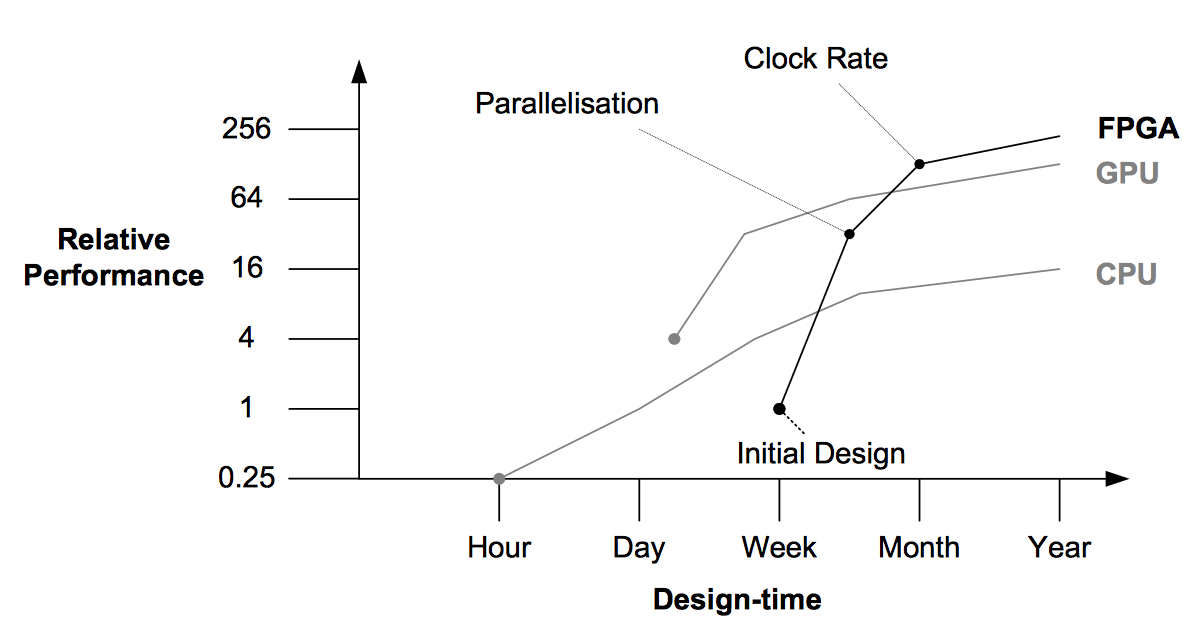
\includegraphics[width=0.70\textwidth]{1-cpu-gpu-fpga.png}
%  \caption{Illustration of relative performance versus the design time of several compute resources \cite{}.}
%  \label{fig:1-cpu-gpu-fpga}
%\end{figure}

%\autoref{fig:1-cpu-gpu-fpga} shows an illustration of the design time of workloads targeted at a CPU, GPU and FPGA versus the relative performance that can be achieved. After one day of development, the reference performance is obtained for the workload targeting a CPU after which it can slowly be improved upon. GPUs on the other hand take only slightly longer to design for, but immediately have large benefits in terms of performance. Finally, FPGAs are the most difficult to design for, since it consists both of hardware and software.
%\todo{- discuss two points in the graph}





\subsection{Application Specific Acceleration}
Two recent trends in the data center allow for a wider diversification of compute resources by introducing application specific accelerators in the form of ASICs and FPGAs.\\
One trend is to use fixed-function ASICs, either tightly coupled on-chip or loosely coupled using an interconnect. On-chip accelerators range from compression to cryptographic engines. An example of a loosely coupled accelerator is Google's recent Tensor Processing Unit (TPU) \cite{tpu}. While fixed-function ASIC accelerators provide a better power efficiency compared to a CPU and free up resources since the CPU is able to off-load work, on-chip accelerators consume valuable chip area while being dedicated to only one function. This renders a fixed-function accelerator useless when the underlying algorithm changes in the (near) future. Besides that, there are multiple time consuming steps in the design cycle of an ASIC that increase the time to market.\\
Another trend is the adoption of FPGAs. While FPGAs might not offer the same level of power efficiency that ASICs do, their (re)configurable nature allows for flexibility and reusability. According to the same study mentioned earlier \cite{amdahl-era}, reconfigurable or dynamic cores can always achieve a higher maximum speedup than asymmetric configurations. While the design cycle of ASICs can be up to several years, FPGAs can be designed in a fraction of that time because layout and fabrication are not required. However, FPGAs are more difficult to use compared to CPUs and GPUs since both hardware and software have to be developed. FPGAs have not invested as heavily in double-precision floating-point pre-integrated units. Therefore they specifically shine in non-floating point compute-intensive workloads, on parallel workloads because of their inherently parallel architecture, and also in network communication related acceleration. Parallelism can be exploited at different levels of granularity and optimized fixed-function hardware accelerates the compute-intensity. %They also have a high IO pin count.
The downside is that an FPGA consists of various pre-defined resources, like memories and DSP slices, that constrain the degrees of freedom of the design. When deployed as a compute accelerator FPGAs have typically been connected using a relatively low-bandwidth and high-latency interconnect, limiting their use for memory-intensive workloads. When deployed as network switches, FPGAs have typically been deployed with very high bandwidth using leadership PHYs (Physical Layers).





\subsection{FPGA Adoption in the Data Center}
\label{sec:adopt}
FPGAs are becoming more interesting for specific workloads in the data center for various reasons. The (re)configurability allows for reuse and on-the-fly adaptation.
%, FPGAs have been shown to outperform other types of compute resources in terms of operations per byte for specific workloads.
In addition, FPGAs are more power efficient than other compute resources. This aspects becomes increasingly important for data center operators to keep the TCO down. Traditional limitations of FPGAs are starting to fade away with recent advancements in interconnect standards and system design.

\begin{itemize}
  \item{\textbf{Interconnect limitations}, such as low bandwidth and high latency, limit FPGAs to parallel and latency-insensitive workloads, because latency of the interconnect is much higher than that of host memory. Upcoming interconnect standards target these limitations.}
  \item{\textbf{Programmability} is limited to the use of hardware description languages. Advancements in software frameworks and high-level language to HDL compilers make FPGA acceleration accessible to software engineers. Also manual data movement between the CPU and FPGA is error prone and slow due to copy operations through memory and driver overhead. The typical off-load programming model is being replaced by a shared memory model with advancements in system design. This enables seamless integration of FPGAs with CPUs and lets the FPGA act as a thread-level functional unit instead. Accessing FPGAs for development becomes simpler by using cloud platforms such as Amazon EC2 F1.}
\end{itemize}

%Traditionally, FPGAs were applied to parallel and latency insensitive workloads, because latency of the interconnect is much higher than that of main memory. This is changing with upcoming interconnect standards such as CCIX, OpenCAPI and PCI Express gen 4.

%Also advancements regarding programmability are enabling adoption. The typical off-load programming model is being replaced by a shared memory model due to advancements in interconnects. This enables seamless integration of FPGAs with CPUs and lets the FPGA function as a thread-level functional unit instead of as an off-load engine.
%Finally, software frameworks have dramatically improved. No longer is the knowledge of an HDL needed, since multiple high-level language to HDL compilers exist. Examples are HLS by Xilinx, Matlab, Haskell, OpenCL, etc. A special framework is SNAP for CAPI 1.0, which extends the interconnect with a simplified API and easily integration of the accelerated function. Another initiative is the Vineyard project, which lets the compiler decide on which compute resource to use, provided that the requested accelerated function is available in their database.

One approach is integration of CPUs with FPGAs, like Intel is doing with their Xeon processors \cite{gupta-xeon}. The FPGA is currently on the same package as the CPU and expected to be on the same die in the future. Such advancements enable a high bandwidth interconnect. Another approach is by using off-chip interconnects to attach FPGAs. We are interested in the latter approach, since such advancements in interconnects are also beneficial for other attached devices.

% The first problem is addressed by a large number of available compilers and frameworks which convert (parts of) higher-level programming languages to HDL. Examples include MatLab HDL Coder, Xilinx HLS for C, C++ and SystemC, CLaSH for Haskell to HDL, OpenCL for C and C++, Reconfigure for Go to HDL and MyHDL for Python to HDL. The attainable performance of these tools might not achieve similar performance as fully custom FPGA designs.

%FROM FRONTIERS PDF chapter 1\\
%This adoption is two-fold. First of all, software stacks to program FPGAs have greatly evolved and nowadays also allow for high-level languages to compile into HDL. Second of all, it becomes more difficult to extract performance out of multi-core CPUs. Small performance jumps are made in every generation, mostly by improving the throughput, but not the single-core performance. REF FRONTIERS\\
%But both FPGA and GPU accelerators offer a more compelling improvement in performance per watt. Hybrid CPU-FPGA and CPU-GPU systems can offer similar performance and performance per watt, at least according to tests that Microsoft has ran, on deep learning algorithms. The GPUs run hotter, but they do roughly proportionally more work and at the system level, offer similar performance per watt.\\
%FPGAs have had a notorious reputation for a long time. They were difficult to program and set up and required an expert to do so. Also the scarce availability of logic resources and memory capacity per card and slow interconnect resulted in only being applicable to specific workloads. Therefore the FPGA was only used in a niche market.\\
%From machine learning, high performance computing, data analytics, and beyond, there is a new day dawning for FPGAs in a more diverse range of application areas. Highly parallel workloads that ca be contained in a small power envelope and take advantage of the growing amount of on-chip memory available on FPGAs are all in the sights of FPGA makers and potential end users.\\
%fpgas can battle for ML with gpus because of their power envelope. however a better fit is cloud computing, but programming difficulty is holding it back.\\
%FPGAs are set to become a companion technology in some hyperscale datacenters, Dhulla says. “We are seeing that these datacenters are separated into ‘pods” or multiple racks of servers for specic workloads. For instance, some have pods set aside to do things like image resizing, as an example. Here they are  nding a  t for FPGAs to accelerate this part of the workload.” In other hot areas for FPGAs, including machine learning, Dhulla says that they are operating as a “cooperating” accelerator with GPUs. “There is no doubt that for the training portion of many machine learning workloads GPUs are dominant. There is a lot of compute power needed here, just as with HPC, where the power envelope tradeoff is worth it for what is required.”\\
%fpgas are very much adopted in financial market due to their good integer performance\\
%seems like fpgas are being used as the glue between the cpu and the gpu. to accelerate very specific parts of a workload.\\
%Over the last year there have been a few highly publicized use cases highlighting the role of FPGAs for specific workloads, particularly in the deep learning and neural network spaces, as well as image recognition and natural language processing. For instance, Microsoft used FPGAs to give its Bing search service a 2X boost across 1,632 nodes and employed a creative 2D torus, high throughput network to support Altera FPGA-driven work. China’s search engine giant, Baidu, which is also a heavy user of GPUs for many of its deep learning and neural network tasks, is using FPGAs for the storage controller on a 2,000 petabyte array that ingests between 100 terabytes to a petabyte per day. These and other prominent cases of large-scale datacenters using FPGAs, especially when they do so over GPUs, are bringing more attention to the single- precision  oating point performance per watt that FPGAs bring to the table.\\
%While some use cases, including the Baidu example, featured GPUs as the compute accelerator and FPGAs on the storage end, Altera, Xilnix, Nallatech, and researchers from IBM on the OpenPower front were showcasing where FPGAs will shine for deep learning in the cloud. The takeaway from these use cases is that the speedups for key applications were hosted inside ultra-dense machines that would melt the Xeon if a GPU was placed in concert. For tight-packed systems, they are a viable choice on the thermal front and even though there might not be as many algorithms where FPGAs can show off (compared to GPUs) this could be the beginning of a golden era for the coprocessors, especially now that there are CAPI and QPI hooks for taking advantage of shared memory on FPGA-boosted systems.\\
%If you ask Altera, Xilinx, and others, this is happening because of what we can call the “three P’s of FPGA adoption” – performance, power, and price. In early 2016, we were able to sync up with several of the main FPGA vendors at the GPU Technology Conference (the irony) and co-located OpenPower Summit, where we heard quite a bit about the golden age of the FPGA—all brought about by the cloud. With an estimated 75 percent of all servers being sold to live a virtualized life, the market rationale is not dif cult to see—but performance per watt is the real story, especially when compared to GPUs, says Mike Strickland, who directs the compute and storage group at Intel/Altera. That puts Strickland in direct contact with HPC and hyperscale shops and gives him an understanding of their architectural considerations.\\
%Although FPGAs have the reputation of being expensive, at high volume they are on par with other accelerators, Strickland explained, pointing to Microsoft as a key example. However, he says that the ef ciencies of the performance boost far outstrip GPUs for neural algorithms, which leads to additional savings. There are numerous charts and arts highlighting the price/performance potential of FPGAs in both bare metal and virtual environments, but the real question is that stubborn fourth “P’ – programming.\\





\section{Interconnect Trends}
In this section, the two typical drawbacks of FPGA adoption are explored in more detail. First bandwidth trends are explored, followed by reported improvements in FPGA programmability. Software framework and high-level to HDL compiler advancements are not discussed further in this thesis.



\subsection{Attached Devices Push Bandwidth Requirements}

%- network: find study of what percentage of network bw is used by which applications.\\
%- network: besides ethernet bw increasing from 10, to 100 to soon 400 Gb/s, how does inifiniband and others fit in? Infiniband is only within or between servers. Not like ethernet.\\

Besides the adoption of various kinds of accelerators in the data center, the balance of bandwidths at system-level have changed significantly in recent years. Advancements in networking and storage result in increased bandwidth requirements of such devices. With the increase in complexity and volume of data center workloads, there is never enough or fast enough storage available.
Emerging workloads, such as big data and machine learning, using data sets in the order of exabytes ($10^{18}$), are good examples of this \cite{teradata}.
%According to EMC\textsuperscript{2}, by 2020 about \SI{1.7}{\mega\byte} of data will be created every second per human \cite{big-data}.
Therefore, new storage protocols are quickly adopted, with NVMe over PCI Express being the latest achieving bandwidths of several gigabytes per device. The previous generation reached only half a gigabyte at best. Network bandwidths are increasing similarly by quick adoption of both the \SI{100}{\giga\bit\per\second} and \SI{400}{\giga\bit\per\second} standards in only a few years time. With more and more data and services moving to the cloud, network bandwidths have to increase rapidly.



\subsection{Bandwidth Trends at Device-Level}
\todo{Ref to Figure 2.1a and 2.1b is incorrect.}

Fritz Kruger, a SanDisk Fellow, collected data regarding DRAM, network and storage bandwidth for a presentation in 2016 and predicted the future until 2020. \autoref{fig:1-fritz} shows his findings, with the addition of PCI Express bandwidth to act as a proxy for interconnect bandwidth. For each generation of the PCI Express standard, the bandwidth of sixteen lanes is plotted, since this is typically the maximum number of lanes per PCI Express device. DRAM is inherently uni-directional and several cycles are required to turn the channel around. A memory controller takes care of this by combining reads and writes to limit the overhead cycles spent in configuring the channel. Therefore, DRAM bandwidth should be interpreted as either a read or write channel with the plotted bandwidth, while attached devices such as network and storage typically have a bi-directional link.\\
The slope of each of the fitted lines is important here. Clearly, both network and storage bandwidths are increasing at a much faster rate (steeper slope) than DRAM and PCI Express. The network and storage slopes are similar and double every 18 months. PCI Express doubles every 48 months while it takes DRAM 84 months to double in bandwidth. A shift in system balance is expected for future systems where DRAM, interconnect, network and storage bandwidth are about the same.\\
The fitted straight lines for each of the four data sets shown in \autoref{fig:1-fritz-bw-log} indicate exponential behavior, which can be clearly seen in \autoref{fig:1-fritz-bw}. This figure shows exactly the same data, but on a linear y-axis instead. While it might look like accelerators, such as GPUs and FPGAs, will have to compete for interconnect bandwidth with network and storage, vendors can always scale memory and interconnect bandwidth accordingly. While scaling is the trend, as becomes apparent from the next paragraph, and works in the short-term, it does not solve the fundamental problem of lacking DRAM bandwidth improvements.\\
The reason that DRAM bandwidth is not increasing at a similar pace is two fold. Typically, the number of channels or the channel frequency is increased. However, each solution has significant implications. Every additional channel requires a large number of pins (order of 100) on the processor package (assuming an integrated memory controller) that increases chip area cost. Increasing channel frequency requires expensive logic to solve signal integrity problems at the cost of area, and more aggressive channel termination mechanisms at the cost of power consumption \cite{dram-1, dram-2}.
%- Why does DRAM bandwidth not double faster? Capacity scaling problem is known (DRAM technology limitations). Question at IBM ARL talk.\\

%\todo{- [Style] Even out subfigure width.\\
%- [Ask] Fit straight line on fig a and exponential curve on fig b.\\
%- [Peter] DRAM and SATA are half-duplex while PCI Express and Ethernet are full-duplex. How to compare?\\ Plotted PCI Express interconnect as uni-directional. Change plot axis names accordingly.\\
%}

%\begin{figure}[H]
%  \begin{subfigure}{0.5\textwidth}
%    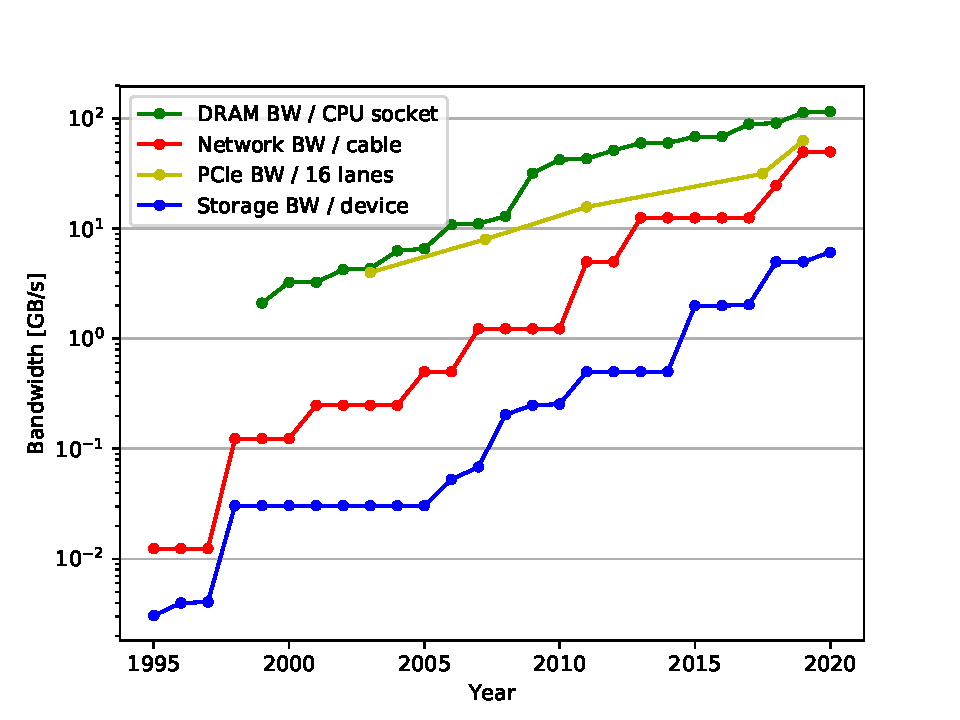
\includegraphics[width=1.0\linewidth]{1-fritz-bw-log.pdf}
%    \caption{Data plotted on a semi-log scale.}
%    \label{fig:1-fritz-bw-log}
%  \end{subfigure}
%  \begin{subfigure}{0.5\textwidth}
%    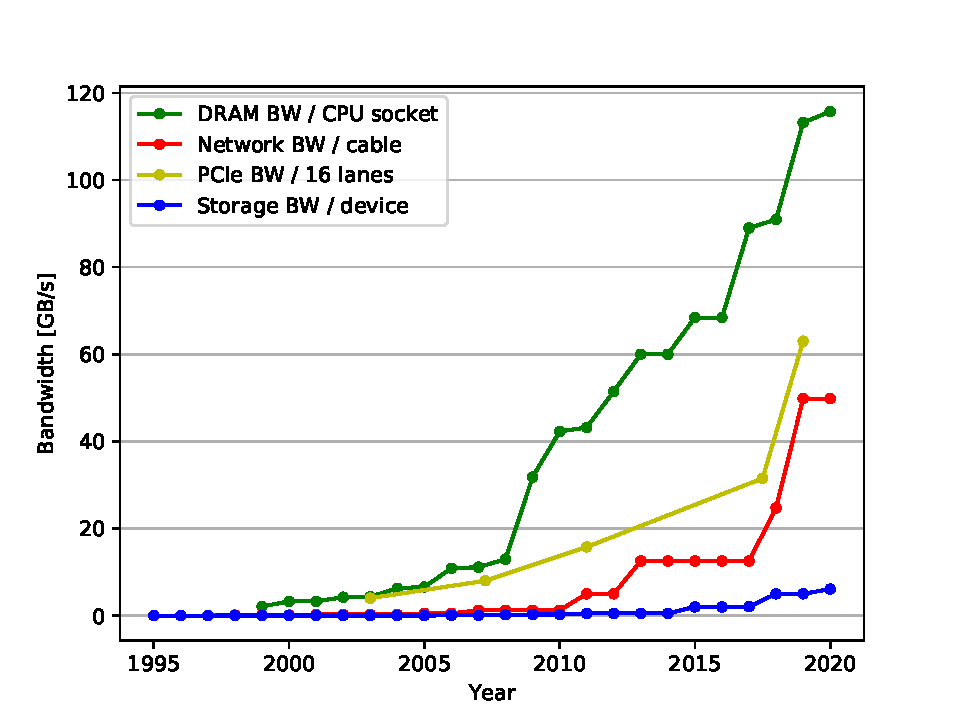
\includegraphics[width=1.0\linewidth]{1-fritz-bw.pdf}
%    \caption{Data plotted on a linear-linear scale.}
%    \label{fig:1-fritz-bw}
%  \end{subfigure}
%  \caption[Bandwidth at device-level trends Fritz reference.]{Bandwidth trends at device-level \cite{fritz}\footnotemark.}
%  \label{fig:1-fritz}
%\end{figure}

\begin{figure}[htb!]
\ffigbox[\textwidth]
  {
    \begin{floatrow}
    \ffigbox[\linewidth]
      {\captionof{subfigure}{Data plotted on a semi-log scale.}
      \label{fig:1-fritz-bw-log}}
      {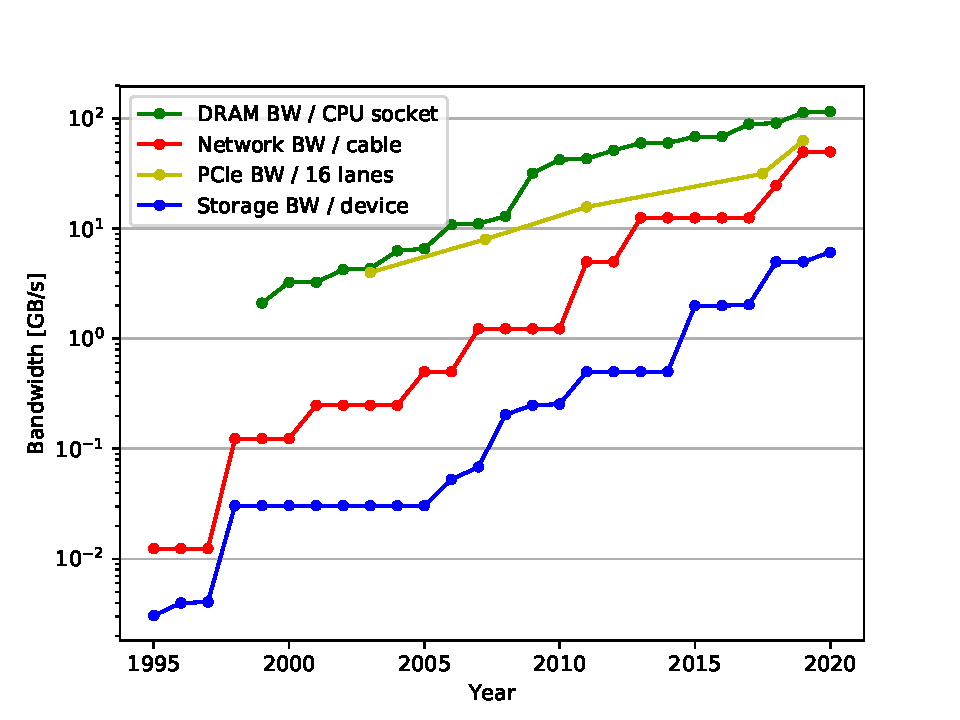
\includegraphics[width=1.0\linewidth]{1-fritz-bw-log.pdf}}
    \ffigbox[\linewidth]
      {\captionof{subfigure}{Data plotted on a linear-linear scale.}
      \label{fig:1-fritz-bw}}
      {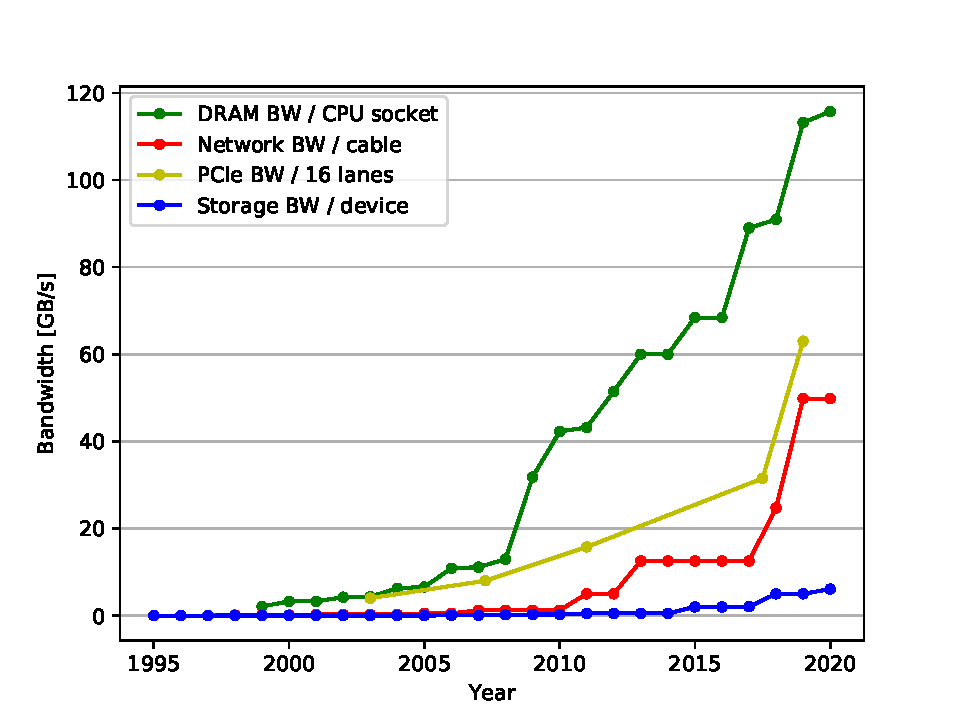
\includegraphics[width=1.0\linewidth]{1-fritz-bw.pdf}}
    \end{floatrow}%
  }
  {\caption[Bandwidth trends at device-level \cite{fritz}.]{Bandwidth trends at device-level \cite{fritz}\footnotemark.}\label{fig:1-fritz}}
\end{figure}
\footnotetext{Data points were approximated from the referenced figures in order to add the PCI Express standard bandwidth and represent all bandwidths in GB/s.}



\subsection{Bandwidth Trends at System-Level}
\label{sec:bw-trends}

%\todo{- [Ask] Finish bandwidth plots.\\
%- [Extra] SPARC CPU info\\ %\url{https://nl.hardware.info/nieuws/53488/oracle-introduceert-sparc-m8-database-processor}\\
%}

In order for vendors to stay ahead of the inevitable crossing of DRAM, interconnect, network and storage bandwidths, scaling is applied to both DRAM and interconnect bandwidth for the short-term. While the previous figures show predictions for future generations, more recent information regarding upcoming or recently released CPUs indicate that there is a large push to more DRAM and interconnect bandwidth. \autoref{fig:1-processor-bw} shows the peak\footnotemark~DRAM and interconnect bandwidth per CPU generation for single socket systems over a span of eight years. Per vendor and generation, the highest rated model is shown. Note that in the case of Intel, the E5 models have more interconnect bandwidth, while the E7 models have more DRAM bandwidth. Unreleased CPUs are plotted at the year 2018.

\footnotetext{The only exception are the IBM POWER8 and POWER9, which state the sustained DRAM bandwidth.}

%\begin{figure}[H]
%  \captionsetup[subfigure]{justification=centering}
  %\centering
%  \begin{subfigure}{0.5\textwidth}
%    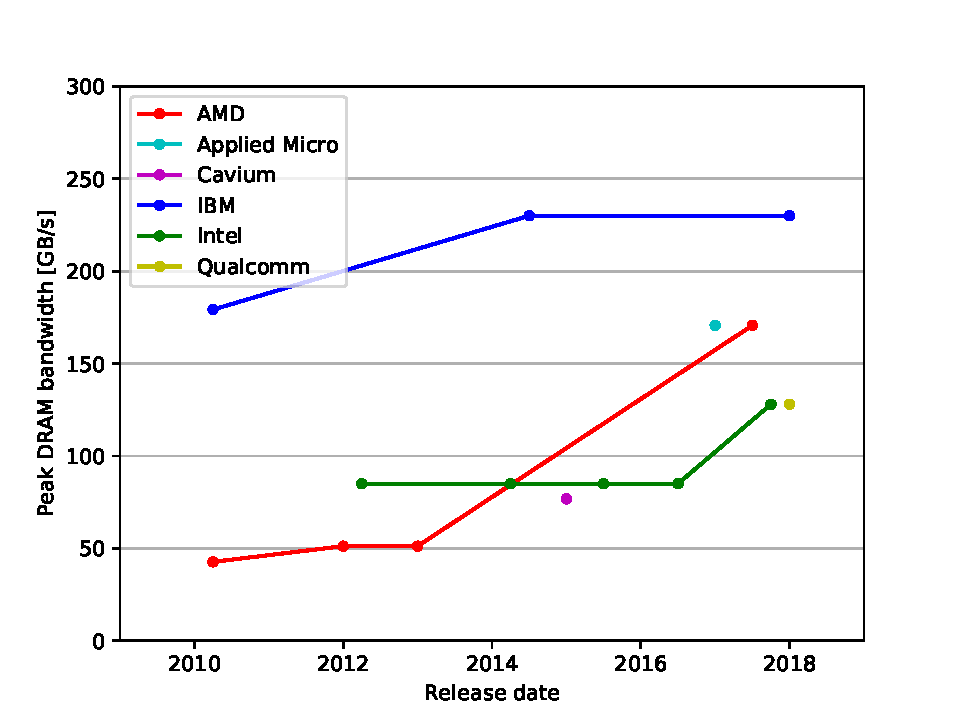
\includegraphics[width=1.0\linewidth]{1-processor-bw-dram.pdf}
%    \caption{Peak DRAM bandwidth.}
%    \label{fig:1-processor-bw-dram}
%  \end{subfigure}
%  \begin{subfigure}{0.5\textwidth}
%    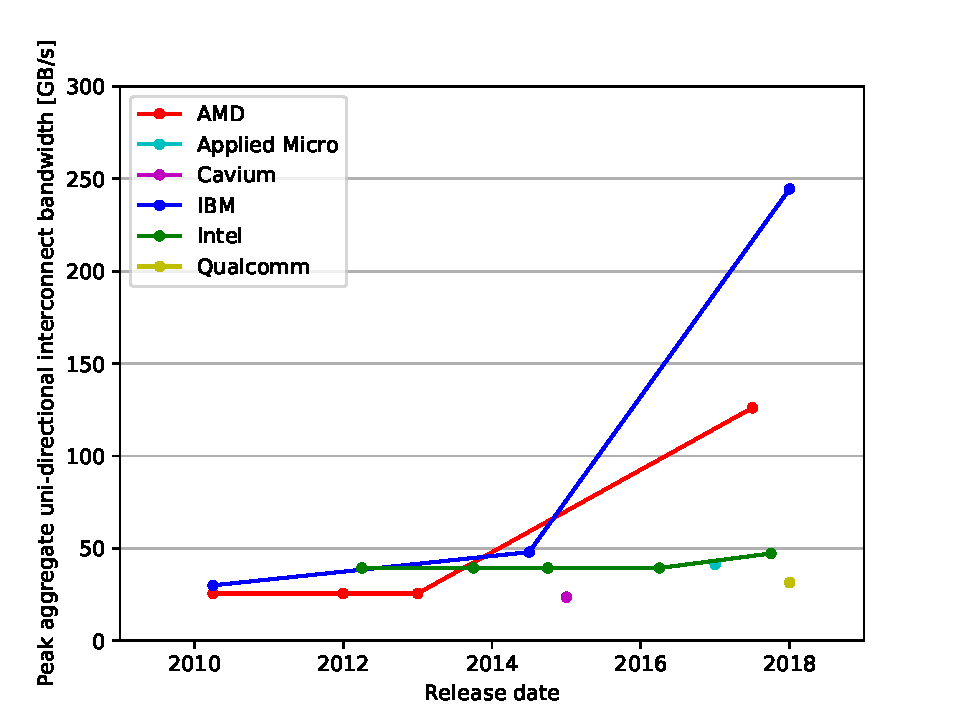
\includegraphics[width=1.0\linewidth]{1-processor-bw-io.pdf}
%    \caption[Peak aggregate uni-directional interconnect bandwidth.]{Peak aggregate uni-directional\\interconnect bandwidth.}
%    \label{fig:1-processor-bw-io}
%  \end{subfigure}
%  \caption{Study of bandwidth trends at system-level for single socket CPUs per generation.}
%  \label{fig:1-processor-bw}
%\end{figure}

\begin{figure}[htb!]
\ffigbox[\textwidth]
  {
    \begin{floatrow}
    \ffigbox[\linewidth]
      {\captionof{subfigure}{Peak DRAM bandwidth.}
      \label{fig:1-processor-bw-dram}}
      {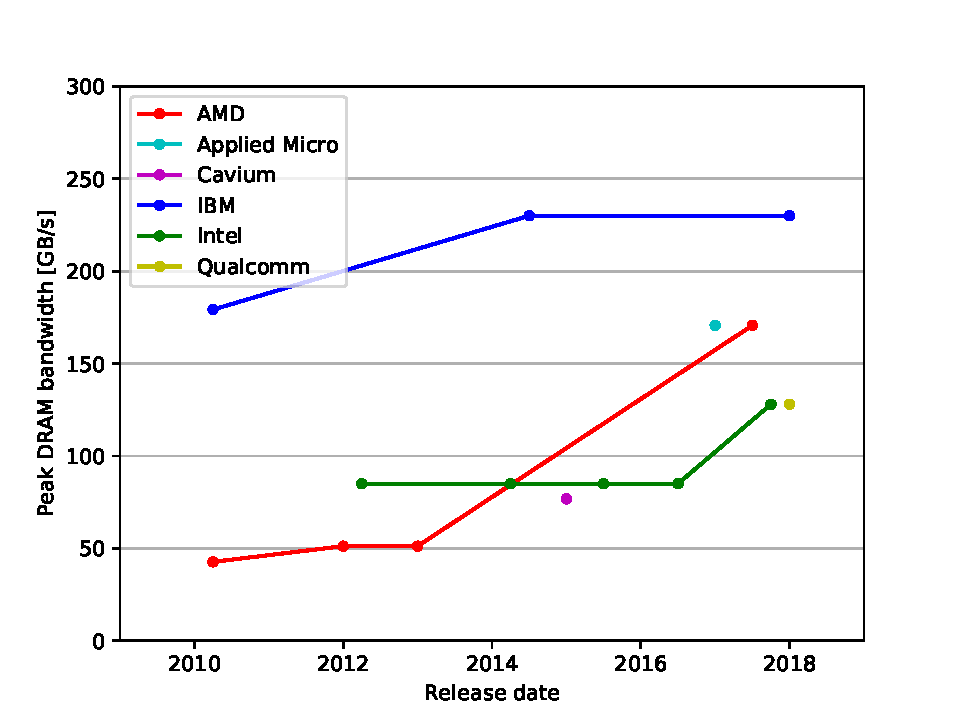
\includegraphics[width=1.0\linewidth]{1-processor-bw-dram.pdf}}
    \ffigbox[\linewidth]
      {\captionof{subfigure}{Peak aggregate uni-directional interconnect bandwidth.}
      \label{fig:1-processor-bw-io}}
      {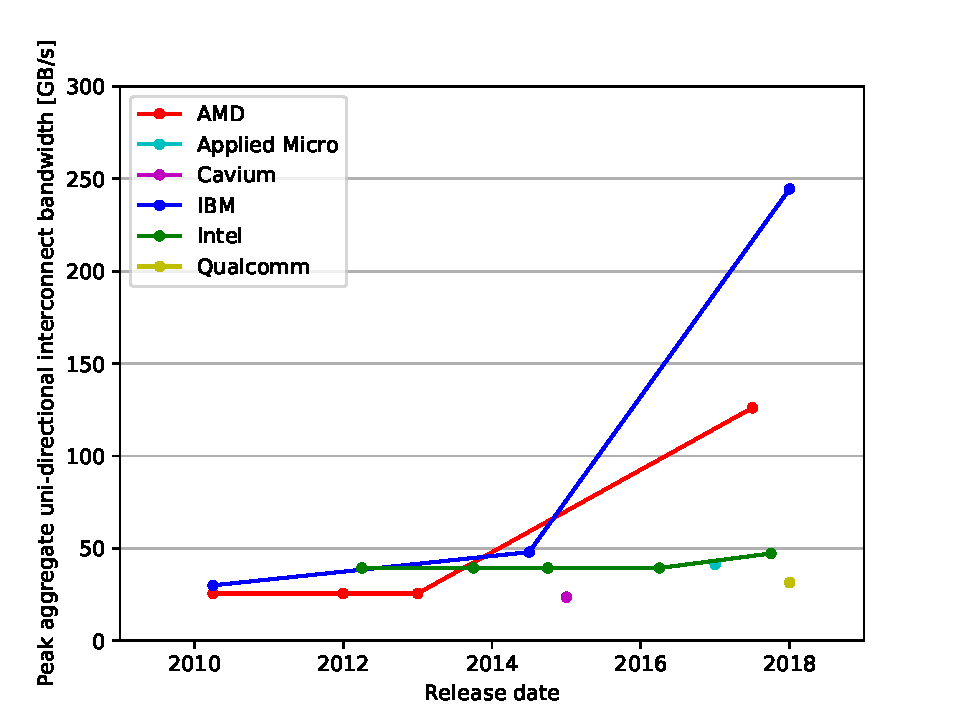
\includegraphics[width=1.0\linewidth]{1-processor-bw-io.pdf}}
    \end{floatrow}%
  }
  {\caption{Study of bandwidth trends at system-level for single socket CPUs per generation.}\label{fig:1-processor-bw}}
\end{figure}



\subsubsection{DRAM Bandwidth Trends}
The DRAM bandwidth data shown in \autoref{fig:1-fritz} was mostly taken from the Intel Xeon product family according to the author \cite{fritz}. \autoref{fig:1-processor-bw-dram} shows that AMD and IBM, compared to Intel, scaled their DRAM bandwidth aggressively by increasing the number of memory channels or by using additional buffer chips between the last-level cache and the DRAM. Only after several years did Intel improve the memory bandwidth in their latest generation by increasing the operating frequency and number of channels. While the Intel Xeon DRAM bandwidth follows the predictions quite well, both AMD's EPYC processors and IBM's POWER8 and POWER9 processor break the trend. The POWER processors offer roughly twice as much memory bandwidth compared to the latest Intel Xeon family.\\
An implication for the slow DRAM bandwidth increase is that flash storage can be attached as accelerator and act as DRAM or local storage for a data intensive accelerator, for example by exploiting data locality.



\subsubsection{Interconnect Bandwidth Trends}
\autoref{fig:1-processor-bw-io} shows the peak aggregate uni-directional interconnect bandwidth per CPU socket. This is calculated as the product of the uni-directional bandwidth per lane and the number of lanes. In the past, nearly every vendor used their own interconnect standard, possibly with a bridge to PCI Express. The general consensus is to use PCI Express and it has become the industry standard. While the introduction of PCI Express Gen 4 took longer than previous generations (see \autoref{fig:1-fritz-bw-log}), initiatives took off to extend the PCI Express standard with coherency protocols for seamless integration of attached devices. IBM started in 2014 with CAPI and more recently the CCIX consortium tries to implement a protocol for current and future PCI Express standards.\\
The aggregate interconnect bandwidth at system-level is increasing by an order of magnitude and has passed DRAM bandwidths. In the latest generation, both AMD and IBM are investing aggressively. AMD scaled the number of PCI Express Gen 3 lanes per socket to 128 lanes. For comparison, the latest Intel processor offers a maximum of 48 lanes for the same PCI Express generation. However, for multi-socket systems the AMD CPU will sacrifice half of its lanes for SMP, while Intel has a dedicated link for that. IBM's upcoming POWER9 processor has almost twice the interconnect bandwidth compared to AMD. This is achieved by having 48 lanes of PCI Express Gen 4 and 48 lanes of a new \SI{25}{\giga\bit\per\second} link called BlueLink. Note that both types of interconnect on the POWER9 can be used for SMP as well. This fundamental improvement enables a massive increase in bandwidth compared to other state-of-the-art systems. Although a significant improvement, it is only a small bump on the log-scale in \autoref{fig:1-fritz-bw-log}.\\
Very recently, new players such as Applied Micro, Cavium and Qualcomm are entering the server processor market with ARM-based processors. Such servers are targeted for cloud, content delivery, storage and web workloads and differ greatly from the traditional high performance and power consuming POWER and x86 architectures. These types of workloads do not require high-bandwidth accelerators, but instead prefer fixed-function on-chip accelerators and integrated network adapters. This class of servers does allow for memory bandwidths similar to those of Intel.

This study shows that the latest generation of processors tries to keep up with the exponentially increasing bandwidth of network and storage by scaling the interconnect in a similar fashion, and no longer follows the tradition shown in \autoref{fig:1-fritz}. It is important that DRAM bandwidth scales as well, in order to not become a bottleneck. Increasing the interconnect bandwidth by an order of magnitude forces us to reconsider design choices for accelerators.





\section{Current Interconnect Bottlenecks}
\label{sec:current}
It has been shown that an increase in interconnect bandwidth is required for emerging workloads in the data center. However, this problem is not solely solved by blindly scaling the current interconnects because the traditional Input/Output (IO) model will become a bottleneck. This section introduces the traditional IO model and its bottlenecks.

%\todo{- [Extra] Explain difference between memory and IO mapped devices. See comments.\\ %Nice picture: \url{https://www.robots.ox.ac.uk/~dwm/Courses/2CO_2014/2CO-N4.pdf}. main point is io mapped is in separate address space (x86 IN and OUT instructions), while memory mapped is in same address space. currently mostly used, io mapped is more for embedded.\\
%}



\subsection{Traditional IO Model}
\label{sec:copies}
Workloads contain serial and parallel components, where parallel components typically benefits from highly parallel architectures as mentioned in Section \ref{sec:hetero}. Due to the need for heterogeneous systems, different compute elements must communicate efficiently without decreasing potential execution speedup.\\
In a traditional IO model, the host processor has a shared memory space across its cores with coherent caches. Attached devices such as FPGAs, GPUs, network and storage controllers are memory-mapped and use a DMA to transfer data between local and system memory across an interconnect such as PCI Express. Attached devices can not see the entire system memory, but only a part of it. Communication between the host processor and attached devices requires an inefficient software stack in comparison to the communication scheme between CPU cores using shared memory.\\
\autoref{fig:2-memcpy} shows the data flow in the traditional IO model. The yellow boxes within the purple physical memories indicate seperate address spaces. In order to offload data from host memory to an attached device, data is copied from the application (\textit{app}) region by the CPU into a pinned (non-pageable) section of the host memory called a buffer. Only the buffer is visible to the attached device (due to different address spaces, therefore different instructions for memory and Memory Mapped IO (MMIO) accesses), because it does not share the same translation tables with the CPU. By reading the buffer, with the help of device drivers, the CPU is able to write the data, across an interconnect, into the local memory of the attached device. The attached device fulfills a certain \textit{Function}, which reads the data from the local memory and processes it. The result will then be written into the local memory after which the \textit{Function} informs the host it has finished. A DMA for example will move the result into a second buffer within the host memory. From here, the CPU copies the data to the application address space after which the application can continue.

\begin{figure}[H]
  \centering
  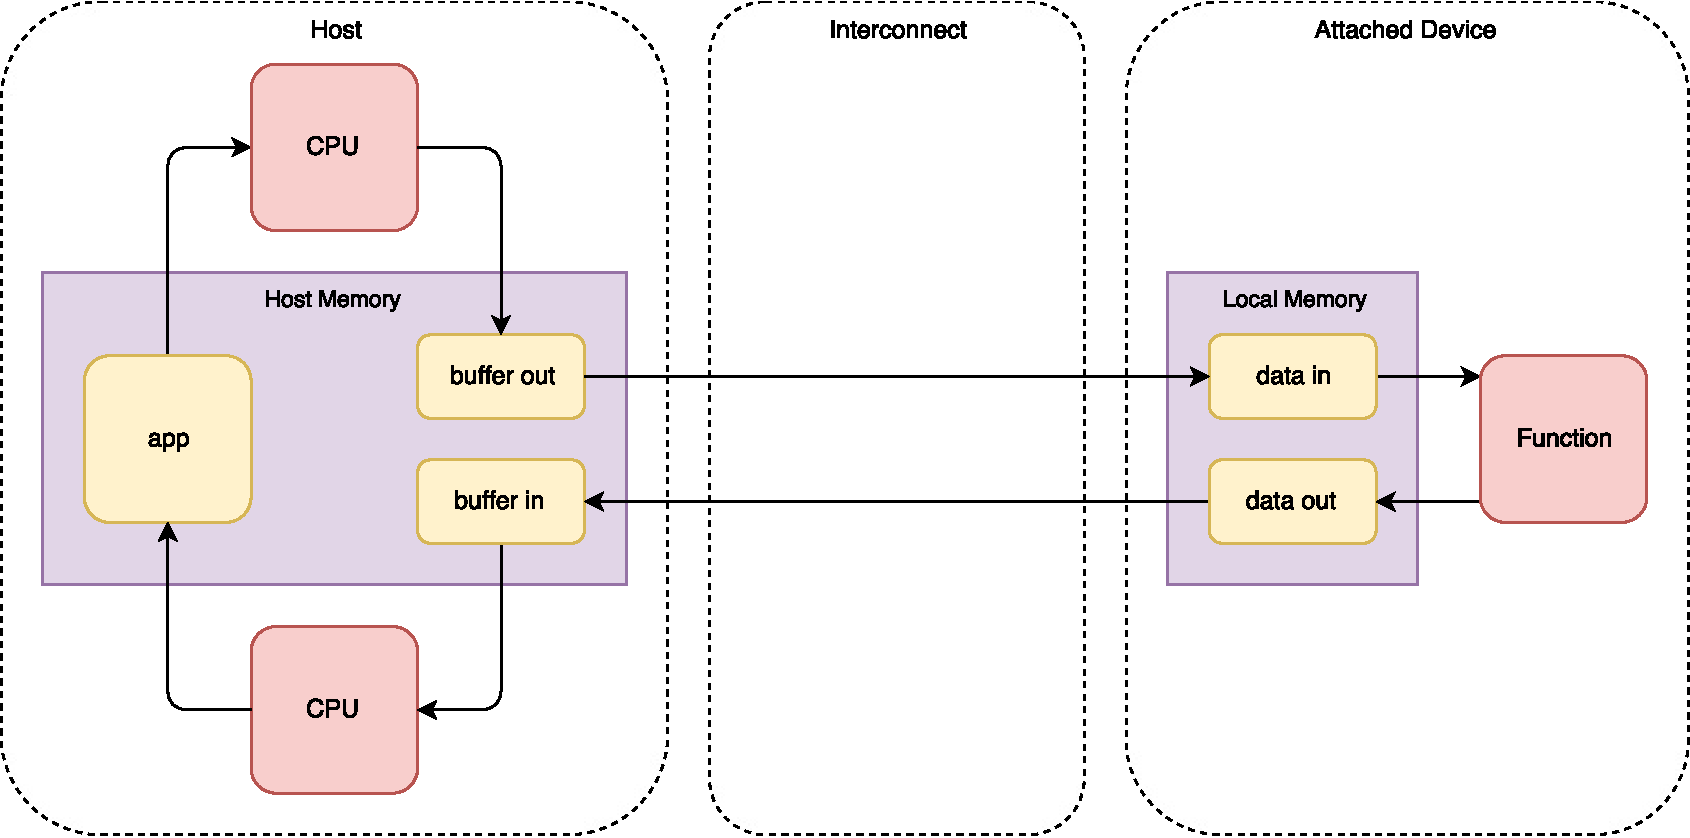
\includegraphics[width=0.80\textwidth]{2-memcpy.pdf}
  \caption{Multiple copy operations in the traditional IO model.}
  \label{fig:2-memcpy}
\end{figure}



\subsection{Communication and Synchronization Overhead}
Communication and synchronization between the host and attached device using interrupts and MMIO operations typically involves the device driver and introduces overhead \cite{capi-zurich}. These communication channels are used to start or stop the attached device.\\
While the attached device is operational, typically the \textit{app} running on the host is idle and waits for the \textit{Function} to finish, after which they synchronize and continue.\\
Functions with a relatively low number of data transformations suffer from a high interconnect overhead per data element with the traditional model. The communication overhead decreases the potential execution speedup, limiting acceleration to data transformation intensive workloads.



\subsection{Host Memory Access Congestion}
Another bottleneck, illustrated by \autoref{fig:2-memcpy}, is the host memory bandwidth for systems with increasing interconnect bandwidth such as the ones shown in Section \ref{sec:bw-trends}. The traditional model requires four memory copy operations, of which the CPU is involved in a total of three reads and two writes across the host memory channel. Since all attached devices can potentially use all of their assigned bandwidth, the host memory channel will suffer from severe congestion for servicing all copy operations. The fact that host memory is inherently simplex and cycles are required to turn the channel around is not beneficial either.



%\subsubsection{Case Study: Intel Xeon Gold 6154}
%To illustrate this problem, \autoref{fig:2-system-1} shows a hypothetical system where host memory, an accelerator (ASIC, FPGA or GPU) and a network and storage controller are attached to the CPU. With the traditional IO model, the attached devices have a separate address space and data exchange happens by copying through memory.\\
%As an example, a closer look will be taken at the highest end Intel Xeon Gold product line, the 6154 \cite{xeon-datasheet} (the Platinum product line contains a buffer chip between the memory controller and DIMMs. Therefore the host memory bandwidth can not be trivially calculated). This processor has six DDR4 memory channels operating at 2666 MHz for a total host memory bandwidth of roughly 128GB/s. The same processor also offers 48 PCI Express Gen 3 lanes, which is a total of 96 GB/s of duplex interconnect bandwidth. Since the host memory bandwidth is larger than the interconnect bandwidth, even if all interconnect devices would copy through memory, no bottleneck should be observed. This is under the assumption that there is no traffic from the CPU itself. Also, the PCI Express bandwidth is given as duplex while the host memory bandwidth is inherently simplex (the bus either services reads or writes).



\subsubsection{Case Study: IBM POWER9}
To illustrate the problem of host memory congestion, the IBM POWER9 processor is chosen as an extreme example. It supports two new high-bandwidth interconnect standards: PCI Express Gen 4 and OpenCAPI. \autoref{fig:2-system-1} shows a hypothetical system architecture where host memory, an accelerator (ASIC, FPGA or GPU), and a network and storage controller are attached to the CPU.\\
A possible system configuration could have host memory attached with \SI{200}{\giga\byte\per\second} of bandwidth and each attached device with roughly \SI{150}{\giga\byte\per\second} of bandwidth. Using the traditional IO model, the IO devices will be fighting for access to the system memory channel. \SI{450}{\giga\byte\per\second} of data is competing for the same \SI{150}{\giga\byte\per\second} memory channel, since data exchange happens by copying through memory.
%Even worse, if all \SI{492}{\giga\byte\per\second} of IO bandwidth is utilized, multiple copy operations have to be serviced by the host memory which has a bandwidth of up to \SI{230}{\giga\byte\per\second}, depending on the configuration (alternative configurations could only have \SI{120}{\giga\byte\per\second} of bandwidth).
Imagine that in this example, memory access requested by the CPU is not even taken into account. The host memory would seriously bottleneck the whole system in this case, as shown in \autoref{fig:2-system-2} where the thick arrows indicate data transfers.\\
A system configuration like this would not be possible with a traditional IO model. The \SI{300}{\giga\byte\per\second} of bandwidth that OpenCAPI provides mitigates the presented bottlenecks by introducing a coherent and shared memory access model to host memory.

%\footnotetext{Only 32 out of the 48 BlueLink lanes present on the POWER9 processor are OpenCAPI capable. The other lanes are reserved for NVLink 2.0. More details can be found in Section \ref{sec:capp}.}

%\begin{figure}[H]
%  \captionsetup[subfigure]{justification=centering}
  %\centering
%  \begin{subfigure}{0.5\textwidth}
%    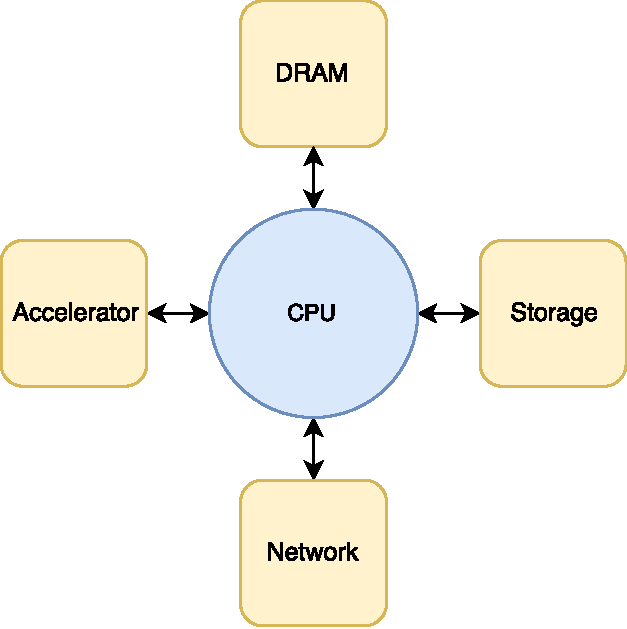
\includegraphics[width=0.90\linewidth]{2-system-1.pdf}
%    \caption{Hypothetical system architecture.}
%    \label{fig:2-system-1}
%  \end{subfigure}
%  \begin{subfigure}{0.5\textwidth}
%    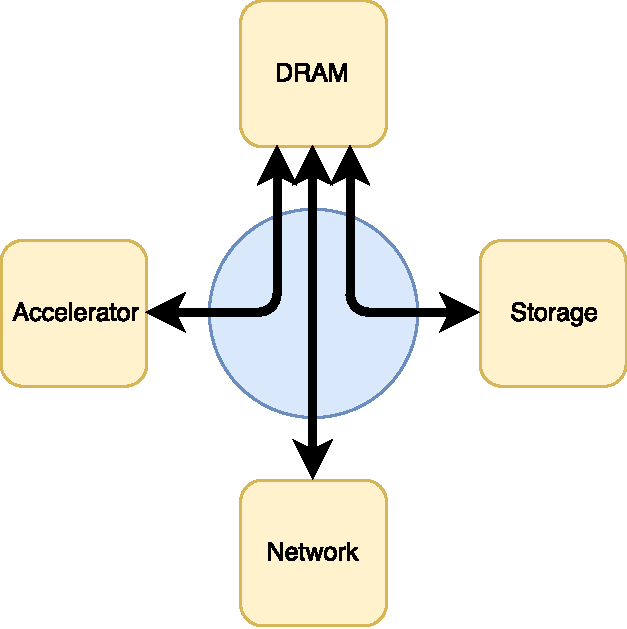
\includegraphics[width=0.90\linewidth]{2-system-2.pdf}
%    \caption{Host memory access congestion.}
%    \label{fig:2-system-2}
%  \end{subfigure}
%  \caption{Hypothetical system architecture suffering from the traditional IO model.}
%  \label{fig:2-system}
%\end{figure}

\begin{figure}[htb!]
\ffigbox[\textwidth]
  {
    \begin{floatrow}
    \ffigbox[\linewidth]
      {\captionof{subfigure}{Hypothetical system architecture.}
      \label{fig:2-system-1}}
      {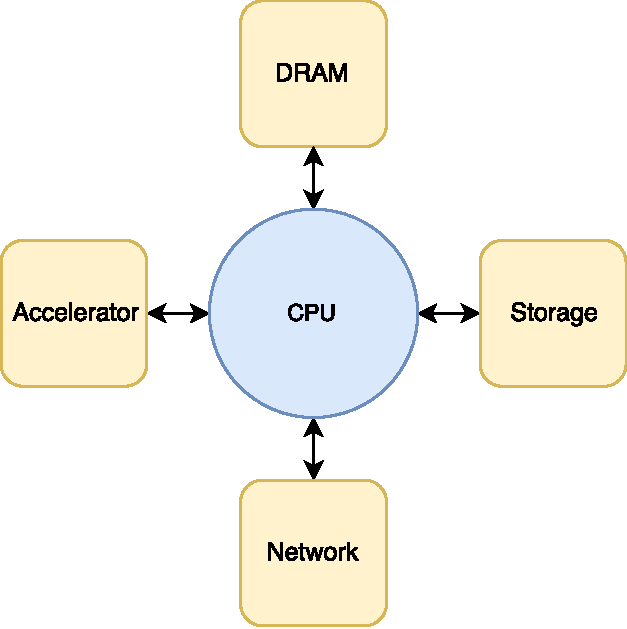
\includegraphics[width=0.8\linewidth]{2-system-1.pdf}}
    \ffigbox[\linewidth]
      {\captionof{subfigure}{Host memory access congestion.}
      \label{fig:2-system-2}}
      {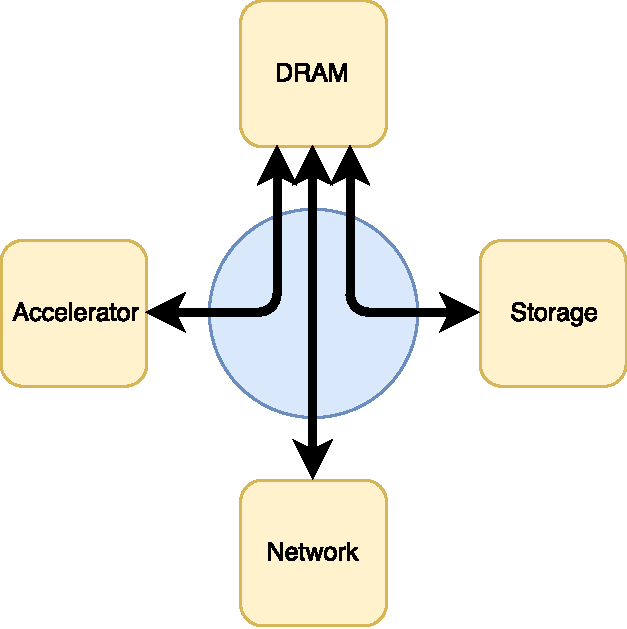
\includegraphics[width=0.8\linewidth]{2-system-2.pdf}}
    \end{floatrow}%
  }
  {\caption{Hypothetical system architecture suffering from the traditional IO model.}\label{fig:2-system}}
\end{figure}





\subsubsection{Case Study: AMD EPYC}
Systems that heavily rely on interconnect bandwidth to improve performance by attaching FPGAs, GPUs, network and storage have to take care that DRAM bandwidth will not become a bottleneck. As shown in Section \ref{sec:bw-trends}, vendors make sure that DRAM bandwidth will not become a bottleneck in the overal system architecture.\\
%Intel's latest generation for example has a DRAM and duplex interconnect bandwidth of \SI{128}{\giga\byte\per\second} and \SI{96}{\giga\byte\per\second} respectively. With a traditional IO model is used, and it probably is, the bottleneck should not be very severe.\\
%IBM's POWER9 processor has a DRAM and duplex interconnect bandwidth of \SI{230}{\giga\byte\per\second} and \SI{492}{\giga\byte\per\second} respectively, where most IO employs a shared memory approach. With the absence of a shared memory space, the DRAM bandwidth would seriously limit system performance.\\
In contrast, AMD's EPYC processor has a DRAM and duplex interconnect bandwidth of \SI{170}{\giga\byte\per\second} and \SI{256}{\giga\byte\per\second}, respectively. Since PCI Express Gen 3 is used, it could very well be that a traditional IO model is used since PCI Express Gen 3 does not support a shared address space between the processor cores and attached devices. If this is the case, system performance could be seriously limited. However, half of the PCI Express Gen 3 lanes can be used for SMP, and this way would remove the bottleneck.





\section{Interconnect Coherency and Shared Memory: A Necessity}
\label{sec:trends-interconnect}
Recent initiatives target the limitations described in Section \ref{sec:current}. Current widely adopted interconnect standards such as PCI Express and AXI are based on the traditional IO model. However, extensions try to improve the usage model. Chapter \ref{ch:state} will discuss the state-of-the-art interconnects in more detail. This section explores necessary changes to the traditional IO model to accommodate for the bandwidth scaling employed by current and future processors.



\subsection{Coherent IO Model}
In order to continue scaling of IO bandwidth to fulfill the requirements of emerging accelerators and attached devices, the traditional IO model has to change and the bottlenecks presented in Section \ref{sec:current} have to be addressed.\\
Shared memory and coherency should be extended to attached devices since accelerators will become an integral part of the ecosystem and should act as a peer to processor cores. System memory should be relieved from performing data copies by employing a shared memory address space between the processor cores and attached devices. Coherency will simplify the programming model for attached devices. Communication overhead can be improved by allowing for shared variables between the host and the attached device in shared memory.\\
The coherent IO model is shown in \autoref{fig:2-desired}. In comparison to the traditional IO model, shown in \autoref{fig:2-memcpy}, there is no CPU involvement and no longer any driver overhead, since copying to buffers is not required. The application has direct access to the address space of the attached device and data exchange is coherent.

\begin{figure}[h]
  \centering
  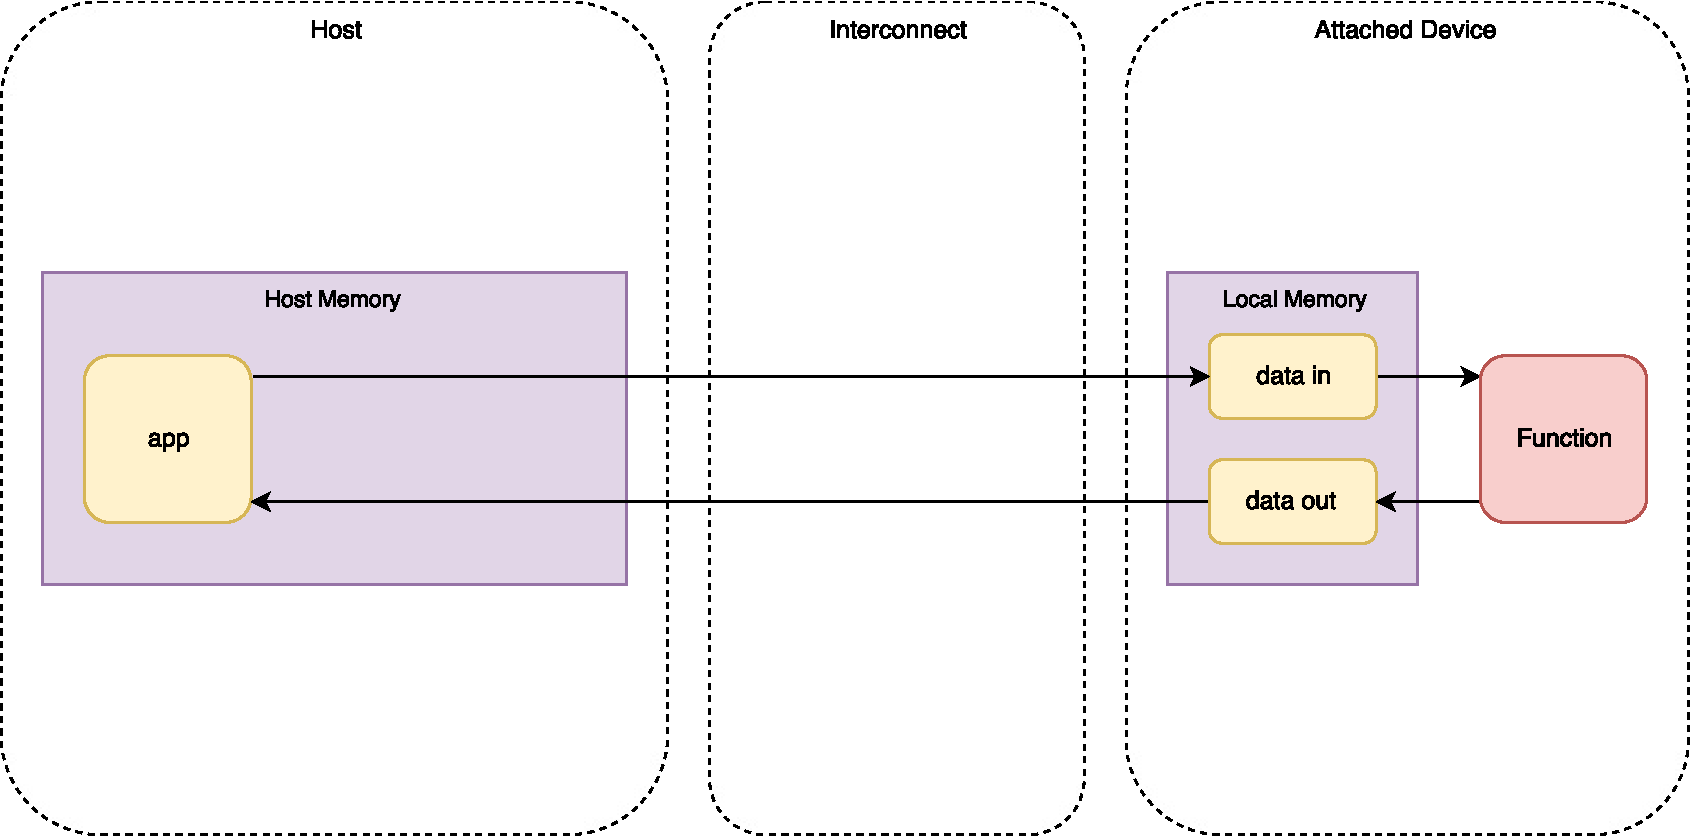
\includegraphics[width=0.80\textwidth]{2-desired.pdf}
  \caption{Coherent IO model.}
  \label{fig:2-desired}
\end{figure}

With the coherent IO model, attached devices are no longer notified using MMIO communication but instead using shared memory. Similarly, completion by the attached device is signaled using shared memory instead of an interrupt for example. By using shared memory, device driver and operating system overhead is decreased significantly.\\
In comparison to \autoref{fig:2-system}, the coherent IO model not only removes the memory copy overhead and therefore avoids memory access congestion, it also allows attached devices to move data between each other without touching host memory. An example could be that data is coming in through a network controller and is immediately moved to an accelerator, as shown in \autoref{fig:2-system-3}.\\
The following sections discuss the required changes for the coherent IO model in more detail.

\begin{figure}[h]
  \centering
  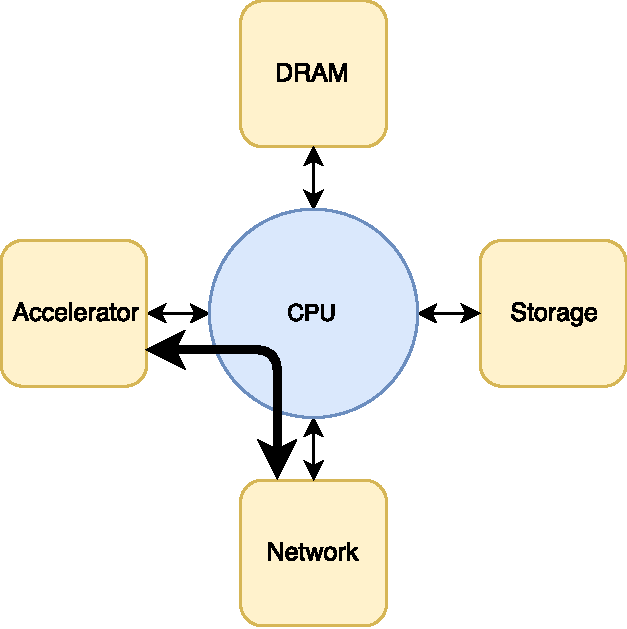
\includegraphics[width=0.4\textwidth]{2-system-3.pdf}
  \caption{Hypothetical system architecture with a coherent IO model.}
  \label{fig:2-system-3}
\end{figure}



\subsection{System-Wide Shared Memory Address Space}

%\todo{- [Extra] What is required in hardware/software for a shared memory address space to work?\\
%}

%\todo{PETER call 29 December. Shared memory and coherence:\\
%- Peter didn’t see this before: key reason for shared memory. if you don’t have shared memory, data structures look different, depending on if host cpu executes it or if accelerator execute it.

%— what do you mean by that? (Yvo asked)\\
%because acc that does not work on coherence memory can’t dereference a pointer. that means that if i have some gigantic piece of code and in the middle i have a function that i want to acc, but i cant, if i want to put it on an acc with PCI Express, i have must make sure i resolve every reference, because acc cant. may not even be possible at compile time to resolve pointers.\\
%to me, its a lot about ease of programming (middle piece of code example; if you have a big piece of code and in the middle you want to accelerate something, you can do that fairly easily with (open)capi. traditional accelerators need more work), in exceptional case where acc has to dereference pointer, it can, just like a thread.
%only thing you have to do, for acc you cant pass arguments through regs. If I am calling a function, here every parameter is on the stack.

%If I am calling a function then, basically if you put all arguments on the stack, then when you call a function the only thing you need to give it is the stack pointer. these days with large reg files, people have calling conventions where a bunch of parameters are also in registers.\\
%if you want to acc with a CAPI attached device, it cant fetch private registers. you have to put all your args on the stack, then you can call an FPGA and act similarly to a thread on a CPU.\\
%no massive restructuring of code, depending on your underlying hardware. very little difference between thread and accelerator. Results in portable code!
%}

Shared memory is an abstraction of a system with multiple physical memory resources and presents these memory resources as a continuous address space. It is desired by programmers to hide details of memory accesses from different physical locations. Without shared memory, data structures look different between the host and accelerator because the accelerator is not able to dereference a pointer. All pointers have to be resolved before sending the code to the accelerator for execution, and this may not even be possible.\\
A shared memory address space will decrease congestion of accessing system memory to result in lower access latency and device driver overhead \cite{capi-cantle}. It also improves programmability since it enables shared buffers (zero-copy) and pointer dereferencing, thus simpler data movement between physical memories (host and device memory). The accelerator acts similar to a processor thread and this allows to easily accelerate a single function in a big application, without having to massively restructure the code.\\
It is obvious that interaction with attached devices using the traditional IO model is not perfect. It requires complex drivers on the host, is error prone due to user data movement, and has a high latency rendering it unpractical for latency sensitive workloads. Shared memory allows the system memory address space to be shared with the IO. This enables for example direct data movement from a network card to a GPU, instead of first copying to main memory or interaction by the CPU. This is achieved by providing the IO with the same address translation tables as the CPU.

%\todo{- [Peter] You can also make a programmability/accelerator transparency argument here.}



\subsection{System-Wide Coherence}

%\todo{- What is required in hardware/software for a coherence to work?\\
%- Is there a significant performance gain or does it only simplify the programming model?\\
%- Why does it enable pointer chasing?\\
%- Important for IO cache coherence: Hennessy page 113: I/O cache coherency question. Page 113: Processor cache coherency is a critical subject in the age of multi-core processors, and we will examine it in detail in Chapter 5.\\
%- Does coherency enable lower latency access to memory? Does it do anything for the memcpy problem encountered before?\\
%}



Caches are widely used in microprocessors and cache hierarchies are becoming larger and more complex, by using various cache levels. By scaling the number of processor cores on a single die, multiple copies of the same data can exist. Cache coherency is required to keep data coherent without any software-intervention. Relying on software to provide snooping, write-back, and invalidation is relatively slow. Hardware-based coherence is preferred since it simplifies the programming model and is faster.\\
%(REF: \url{http://compgroups.net/comp.arch/PCI Express-cache-coherent/191462}).\\
Currently, without coherence, the user has to take care of moving data between resources manually, which is error prone. Typically, data is transferred to the accelerator and the application waits for an interrupt signal from the accelerator to signal completion. The application fetches the result from the accelerator across the interconnect. Caches have to be flushed before other resources can access the data. The FPGA feels more like an off-load engine instead of an extension to a thread running on the CPU.\\
With coherency, a consistent view of memory contents by all participants (CPU cores and IO devices) is guaranteed. Attached devices operate natively within the application’s user space and coherently with the host CPU. This allows attached devices to fully participate in an application without kernel involvement or overhead \cite{opencapi-enablement}.\\
With software coherence, a large burden is placed on the application, drivers and OS to manage timed cache cleaning, maintenance and invalidations. Such operations take time and effort (cache contents have to be written out to system memory). Since caches are invisible to software, managing all of these copies in software is difficult. Keeping caches coherent in software means that all caches have to be flushed \cite{axi-coherence}.\\
Hardware coherency removes the software challenges and makes sharing transparent to the application, at the cost of additional memory traffic between caches about the state of their contents in order to keep all of them synchronized.\\
Coherency also enables new types of workloads such as pointer chasing, but is not truly required. It does significantly simplify the programming model by providing synchronization between the host and attached device mechanisms in hardware or software, therefore making slow interrupt-based solutions obsolete.



\subsection{Thread Synchronization}
Before the usage of accelerators and other attached devices was as common as today, multiple processor cores were used to exploit workload parallelism. Such workloads typically make extensive use of synchronization operations such as barriers, mutexes and semaphores. Therefore, when attached devices act as a peer to processor cores, it makes sense to employ similar synchronization operations. By doing so, notifications using interrupts can be avoided and makes porting existing multi-threaded workloads easier. Instead, the host and attached device communicate through shared variables in shared memory \cite{intel-white}.\\
A lock operation could be implemented from which more complex synchronization operations can be built. Recent interconnect standards incorporate more complex atomic operations to replace the lock operations.\\
Another benefit of moving away from interrupt-based synchronization is that the number of hardware interrupt signals no longer limits the number of interrupts, since interrupts are handled using shared memory. This solution scales much better.





\section{Preliminary Concluding Remarks}
Emerging workloads require a change in system architecture. A diversification of compute resources enables speedups not possible with a single type. The adoption of FPGAs is slow due to interconnect limitations and a complex programming model. To address these issues, attached devices are required to be tightly coupled with the host processor at memory-like bandwidths. Currently, this is not the case and interaction with attached devices involves unnecessary overhead. By extending the shared memory space and coherence domain across the interconnect, attached devices act as a peer to the processor cores. This simplifies FPGA acceleration and enables new usage models. Chapter 3 takes a closer look at state-of-the-art interconnect standards and evaluates the current state of the interaction between the host and attached devices.



% More information:
% CUDA used to have pinned functions. Now is able to immediately instantiate a buffer. Also Unified virtual addressing (UVA) is interesting.
% Directly instantiate buffer: https://devblogs.nvidia.com/parallelforall/how-optimize-data-transfers-cuda-cc/
% UVA: http://docs.nvidia.com/cuda/gpudirect-rdma/index.html#basics-of-uva-cuda-memory-management
% UVA: http://docs.nvidia.com/cuda/cuda-c-programming-guide/index.html#um-unified-memory-programming-hd
% cudaMalloc, cudaMemcpy, etc example: http://developer.download.nvidia.com/CUDA/training/GTC_Express_Sarah_Tariq_June2011.pdf
% Important from previous source: Host pointers point to CPU memory. May be passed to/from device code. May NOT be dereferenced in device code. Same holds for device.
% CPU-GPU data flow: https://gamedev.stackexchange.com/questions/66543/cpu-gpu-memory-data-flow

%\todo{
%- Nice to refer back to earlier in intro for moving to SMP and hetereo. Talk first about moving to SMP requires shared memory to share data between threads, each running on a separate physical CPU core (more on page 348 "In both ... address space is shared". Read more around these pages) and cache coherence. Shared memory for SMP (limit to SMP, no DSM) with caches requires cache coherence (page 351 section 5.2); basic protocols are bus snoop, but scales bad, or directory based, but more complex.\\
%- Check "POWER8 CAPI Education What is CAPI x.pdf" slide 23 and more for general benefits of CAPI and therefore this described new system architecture of tighter coupling of accelerators.\\
%- Hennessy: in age of multi-cores, coherency is important.\\
%Page 346 has general multiprocessor approach and memory organization.\\
%Page 348 "The term shared memory associated with both SMP and DSM refers to the fact that the address space is shared."\\
%Page 352: What Is Multiprocessor Cache Coherence?\\
%Page 386: Synchronization: The Basics, such as atomics.\\
%Read 5.10 Concluding remarks.\\
%}

%\todo{
%- Where is the DMA located in the system? On the CPU, every attached device? See Operating Systems/ I/O Systems pdf.\\
%- Does every attached device have a DMA to master the bus? For example, CPU invokes DMA transfer to GPU. When kernel is done, GPU invokes DMA?\\
%- When CPU moves data from system memory to device, will the DMA on the CPU or on the device be used to handle the transfer?\\
%- Why is the entire system memory not visible to memory-mapped IO devices?\\
%- Why is pinned memory visible to memory-mapped IO devices?\\
%}

%\todo{
%- Great slides on PCI Express versus CAPI and need for shared memory: Enabling Coherent FPGA Acceleration - Allan Cantle\\
%- Typically this happens: pin buffers, translate, map DMA, start IO. Source: Peter Dagstuhl slides.\\
%- Onur Mutlu: Typical system nowadays with memory, CPU, DMA, IO (section 2): \url{http://www.pdl.cmu.edu/PDL-FTP/Storage/decoupled-dma_pact15.pdf}\\
%- Typical CPU-IO interaction: \url{https://stackoverflow.com/questions/11355426/gpu-system-memory-mapping}\\
%}

%\todo{
%- (distributed) shared memory (DSM) model, therefore numa model as well\\
%- importance of (cache) coherency / bus snooping for dsm\\
%- Peter - show conventional way, anything you attach, fpga, network, storage, needs to be copied through memory buffer. this is sum of all io bws added together. like 600GB/s. much more than memory bandwidth of 230GB/s. therefore your memory bw will seriously limit your performance.\\
%- Peter - not everything can copy through memory, too much bandwidth from all attached devices. Much faster to go from network to compute resource for example which will use it directly. No copying needed. This is enabled by (Open)CAPI. If you copy everything through memory, there is just not enough bandwidth to service all other interconnects at the same time. CAPI provides shared address space with main memory which enables that this copying is no longer needed. usually you pin everything in buffer in main memory. then device can see the data (device is io mapped). device doesnt have the same translation tables. Check micro50 slides, peter will probably add something about this. coherency has nothing to do with this. how does coherency then impact the total system?\\
%}

%\todo{
%- Main memory in parallel computer is either shared memory or distributed memory - wiki parallel computing.\\
%- In order to speed-up access, we’ve long used caching to store key data closer to the processor than main memory. When multiple CPUs share a common memory space, they can achieve higher performance if they can use hardware to communicate the cached and/or cacheable state of pieces of that memory. By doing this, each CPU can safely work on a portion of a common dataset without having to use slow software semaphores to control access. If CPU A has cached a piece of memory, it can ensure that CPU B does not modify that same memory space or use an out-of-date copy of the data. To better understand cache coherency, let’s look at a commonly used coherence protocol known as MESI, which refers to the four possible states of a cache line: Modified, Exclusive, Shared, or Invalid. source is 'Using CCIX to implement ...'\\
%- Peter question: if FPGA would have HBM mapped into address space for example, would this be a distributed shared memory system?\\
%- Peter question: for shared memory, do you need both hardware and software to enable it? CUDA has unified virtual addressing for example.\\
%- read: Evaluating cache coherent shared virtual memory for heterogeneous multicore chips PDF.\\
%- News: Linux 4.14 supports heterogenous memory management (HMM) \url{https://tweakers.net/nieuws/131775/linux-414-komt-uit-als-volgende-lts-kernel.html}\\
%}

%\todo{
%- Peter: What else is needed for shared memory to work?\\
%- Peter: Do you call this zero-copy?\\
%- Peter: if FPGA has HBM, can you attach that as well to the address space?\\
%- Peter: address are virtual in P9, is it then shared virtual memory?\\
%}

%\todo{
%- shared virtual memory slides: %\url{http://events.linuxfoundation.org/sites/events/files/slides/Shared%20Virtual%20Memory%20%28SVM%29%20in%20Xen.pdf}\\
%- OpenCL 2.0 shared virtual memroy: %\url{https://software.intel.com/en-us/articles/opencl-20-shared-virtual-memory-overview}\\
%- AMD Fusion slides, zero-copy, CPU-GPU memory sharing: %\url{http://developer.amd.com/wordpress/media/2013/06/1004_final.pdf}\\
%- memory sharing; unified address space amongst cpu and accelerators, even hbm on fpga for example.\\
%- POWER9-VUG pdf (page 19) and CAPI demo pdf (page 5) talk about memory sharing\\
%- Zero-copy data transfers allow for moving data without interaction from the CPU. This not only frees up CPU time and resources, but also reduces latency. While several processors have implemented shared memory, only the recently released SNAP framework by IBM for the POWER8 processor implements the hybrid model of computation mentioned earlier Intel has similar plans for their FPGAs.\\
%}

%\todo{
%- Peter: What is the difference between cache and memory coherence? CAPI has cache coherence but OpenCAPI only system memory coherence. How does that work? Probably coherent memory is that atomic ops are available from the attached device to main memory. Coherent cache is a local cache for the attached device which is coherent with main memory data and other caches.\\
%- Peter: show synchronization example? Naive way which doesnt work, then locks (software), then atomics (hardware).\\
%- problem with multi-thread; mutex/sync with lock and atomics using example. Source with mutex/sync example: \url{https://en.wikipedia.org/wiki/Parallel_computing} at header "Race conditions, mutual exclusion, synchronization, and parallel slowdown"\\
%- Today, atomic transactions are supported for synchronization without using an interrupt mechanism. In emerging applications where math co-processing, visualization and content processing are required, enhanced synchronization would enable higher performance. \url{https://www.embedded.com/design/connectivity/4008241/1/PCI-Express-Gen-3-Simplified}\\
%- Peter: Typically bus-snooping doesn't scale well. How is that solved in the P9?\\
%- Lot of info on cache coherence protocols in Quantitative Approach Chapter 5.\\
%- Must check every place there may be a valid copy, results in a snoop.
%- Snoop filters reduce communication by tracking cache contents \url{http://www.arteris.com/hubfs/2016-05-24-arteris-ncore-overview-PDF-FINAL.pdf}\\
%}

% SOFTWARE FOR FPGAS
%The shift from a traditional CPU-only server, to a CPU and GPU server, to a system consisting of CPUs, GPUs and FPGAs forces the current model of computation to change, both in terms of hardware and software. The typical off-load model of computation used in CPU and GPU systems, where highly parallel data-intensive workloads are taken care of by the GPU while the CPU waits, does not scale well with the addition of more heterogeneous accelerators such as FPGAs. A hybrid model is desired where each part of a workload is mapped onto the compute resource that fits the requirements best. The compute resource selection could be based on different requirements such as power efficiency, lowest latency, currently free or under-utilized resources and more.

%\todo{- rethink what i want to say in this section, especially with respect to requirements for improving adoption of accelerators\\
%- Intel-Alterra FPGAs: fpga in package with already hot xeon, what is fpga/xeon performance in terms of heat dissipation (might be much worse compared to loosely coupled fpga, speculation from my side, source would be great. Also bandwidth numbers would be interesting for comparison) limits the size and frequency of such an on-chip FPGA and large accelerators might not even fit. Having high IO for ASICs and FPGAs solves this problem with OpenCAPI 3.0.
%}
%In order to improve integration of FPGA accelerators and fully utilize their potential, coupling using high bandwidth links is crucial. Especially in the hybrid model of computation where algorithms use fine-grain interactions between all compute resources. Currently this high bandwidth link is realized in one of two ways. By acquiring Altera in 2015, Intel plans to use tightly-coupled FPGAs on-?(chip or die) in their Xeon processors. By having the FPGA close to the CPU, a high bandwidth link is used such that the FPGA can act similarly to a functional unit within the CPU to enhance single thread performance. Other companies are adopting loosely coupled FGPA accelerators by using PCI Express interconnect or the upcoming OpenCAPI interconnect. This enables FPGA acceleration for the system as a whole. Indifferent of how the FPGA accelerator is coupled, all companies agree on a coherent, low latency interconnect (ref intel and opencapi).\\
%Besides raw bandwidth, FPGA accelerator adoption is also driven by less programming effort. In order to achieve that, the following two main problems have to be solved.
%\begin{itemize}
%  \item{Enable high-level languages to be converted into HDL to easily exploit FPGA acceleration by non-hardware engineers.}
%  \item{Simplify the programming model by using shared virtual memory.}
%\end{itemize}

%The first problem is addressed by a large number of available compilers and frameworks which convert (parts of) higher-level programming languages to HDL. Examples include MatLab HDL Coder, Xilinx HLS for C, C++ and SystemC, CLaSH for Haskell to HDL, OpenCL for C and C++, Reconfigure for Go to HDL and MyHDL for Python to HDL. The attainable performance of these tools might not achieve similar performance as fully custom FPGA designs.
%The second problem requires hardware changes to the CPU and allows programmers to implicitly move data using pointers. Zero-copy data transfers allow for moving data without interaction from the CPU. This not only frees up CPU time and resources, but also reduces latency. While several processors have implemented shared memory, only the recently released SNAP framework by IBM for the POWER8 processor implements the hybrid model of computation mentioned earlier Intel has similar plans for their FPGAs.

%\todo{Heterogeneous software frameworks:\\
%- maybe say something about different heterogeneous models of computation. then use software frameworks as well. preferably those that allow to program for mixed hardware, like cpu, gpu, dsp, fpga etc\\
%- framework for fpga acceleration: The Xilinx Reconfigurable Acceleration Stack is targeting the markets for machine learning, video transcoding and SQL queries for data analytics. (Source: Xilinx.)\\
%}

  \chapter{State-of-the-Art Interconnects}
\label{ch:state}
Nowadays the Peripheral Component Interconnect Express (PCI Express) and AXI are the interconnect industry standard for PC and server systems, and embedded platforms, respectively. Recently, three open initiatives were announced: CCIX, Gen-Z and OpenCAPI. These open standards are all driven by ISA-agnostic tighter coupling of processors and accelerators, by enabling direct memory access between compute resources and reducing data movement. Also new and emerging memory and storage technologies are exploited \cite{benton}.\\
This chapter focuses on interconnects targeted for accelerators, network, and memory and storage solutions. However, specific memory and storage features of such interconnects will not be discussed. Also interconnects tailored for specific domains such as Ethernet and InfiniBand for networking, NVLink for GPUs and Gen-Z for storage are not discussed, nor are SMP protocols.

%\todo{
%- research transactional memory, would it solve some problems? allows for load/store ops to execute atomically. interesting for parallel systems.\\
%- decide on model of the system, see comparison paper and CAPI UG (asynchronous pull model by afu). OpenCAPI diverted from these models in the architecture because not everyone was using them. So now the philosophy is to let the AFU designer choose the WED model of operation. More info in email conversations with Curt.\\
%- Section on the WED model and other parallel models. Also compare to other accelerator programming models such as CUDA.\\
%- Interesting aspect is how FPGA acceleration looks like for a programmer. What is the typical programming model / paradigm? Or is this captured in 'Need for Shared Memory and Coherence' section? CAPI uses WED, PCIe uses DMA I think, OCAPI uses nothing in particular.
%}





\section{PCI Express}
PCI Express has been around since 2003 and gone through several generations. The PCI-SIG is a group of over 900 companies that maintain the standard. Currently the most widely adopted generation is number three and generation four compliant devices are slowly being released. The remainder of this section briefly explains the architecture of PCI Express and summarises key features of current and future generations.

%\todo{
%- pcie endpoint: is the cpu always the master of the pcie bus, or can a gpu for example also take over? or is it not master-slave style? i remember they always talk about endpoints of pcie root complex.\\
% Endpoint can be the bus master, some information can be found here: \url{https://forums.xilinx.com/t5/Welcome-Join/how-does-a-PCIE-endpoint-recived-master-privilege/td-p/779945}.\\
%- PCIe protocol overview: \url{http://www.ni.com/white-paper/3767/en/}: "The run-time software model used by PCI is a load-store, shared-memory model, which is maintained within the PCI Express architecture to enable all existing software to execute unchanged.".\\
%}



\subsection{Architecture}
This section explains the architecture of PCI Express Gen 3 and later, since various changes have been made at the packet level compared to previous generations of PCI Express which will not be discussed.\\
PCI Express is a packet-based, split transaction protocol with a point-to-point or switched topology. Split transaction means that a request and response are separated by time. Each device is connected to the root complex. The root complex is the root of the IO hierarchy and is connected to the processor and host memory. A PCI Express bus link supports full-duplex communication between two endpoints, with no inherent limitation on concurrent access across multiple endpoints. It uses credit based flow control and typically each link consists of one, four, eight or sixteen lanes. Legacy PCI features are backwards compatible with PCI Express.



\subsubsection{Protocol Description}
The PCI Express architecture consists of three logical layers called the Transaction Layer, the Data Link Layer, and the Physical Layer \cite{pcie-intel}. \autoref{fig:3-pcie} shows a layering diagram and the receive (RX) and transmit (TX) channels of the architecture. Each layer will be briefly discussed.\\
PCI Express uses packets to communicate between participants of the link. Packets are formed in the Transaction Layer and are extended with additional fields when passing through other layers. These additional fields contain information required by other layers to handle the packet appropriately. The receiver of a packet removes these fields in reverse order and uses the information.

\begin{figure}[H]
  \centering
  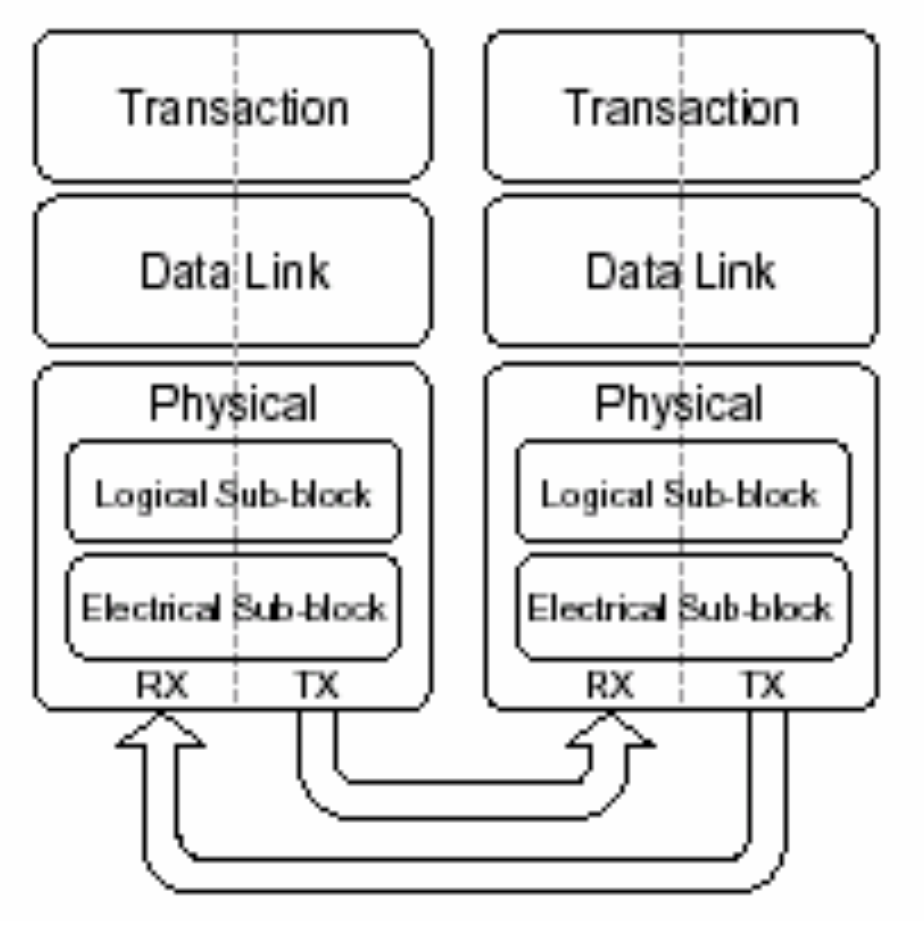
\includegraphics[width=0.40\textwidth]{3-pcie.png}
  \caption{Layering diagram of the PCI Express standard \cite{pcie-intel}.}
  \label{fig:3-pcie}
\end{figure}

\autoref{fig:3-pcie} shows the layering diagram of the PCI Express standard. The Transaction Layer is the top layer and assembles and disassembles Transaction Layer Packets (TLPs). TLPs are the packets used to communicate information and data between two endpoints and consist of a header and data part. Also flow control is managed by using a credit-based scheme and ensures that TLPs are only transmitted when a buffer is available on the other endpoint. This eliminates wasting bandwidth on packet retries due to resource constraints.\\
The Data Link Layer is the middle layer and tags TLPs and handles error detection and correction. The transmission side of this layer pre-pends a sequence number (tag) to the TLP and appends a CRC field to it. The receiving side validates the sequence number, by checking if it is continuous with the sequence number from the previous TLP. It also validates the data by checking the CRC. If the TLP is valid, an acknowledgement (ACK message) is sent to the transmitter. If one or both are invalid, a NAK message is sent and re-transmission of all TLPs starting from the invalid one is requested. The ACK and NAK messages are communicated between layers as Data Link Layer Packets (DLLPs).\\
The Physical Layer is the lowest layer and consists of both electrical circuitry, such as a serialiser/deserialiser (SerDes), and logical components to initialize the interfaces. A lane between two endpoints consists of two unidirectional differential signalling pairs and multiple lanes can be bundled together to form a link.



\subsubsection{Cache Coherency Snooping}
Originally proposed as an extension to PCI Express Gen 2, TLP Processing Hints (TPH) \cite{pcie-tph} provide hints for the host to improve memory access performance by taking the cache hierarchy into consideration. This is done by providing several bits in the TLP. The host snoops memory access requests from PCI Express attached devices to enforce cache coherency by hardware \cite{pcie3}.\\
However, these snoop hints are not required for every memory access request. An example is when a speculative read-ahead buffer is used by the operating system to access storage. Snooping this data could pollute host caches and, therefore, the TPHs can be configured on a per packet basis \cite{pcie3-intel}.

%\todo{
%- "standford ee282 lecture 9" page 24 shows what cache snoop does.\\
%- PCIe Gen 3 spec: page 76 talks about cache coherence (snoop).\\
%- PCIe supports memory request snooping in order to keep CPU caches coherent. \url{https://www.embedded.com/design/connectivity/4008241/1/PCI-Express-Gen-3-Simplified}\\
%- Caching hints explanation: \url{https://www.intel.sg/content/dam/doc/white-paper/pci-express3-accelerator-white-paper.pdf}\\
%}



\subsubsection{Address Translation Services}
Another extension proposed for PCI Express Gen 2 are the Address Translation Services (ATS) \cite{pcie-ats}. This extension was included in the PCI Express Gen 3 specification and translates untranslated addresses to physical addresses. ATS enables attached devices to request address translation from the host in advance to alleviate potential congestion during times with intensive communication across the interconnect \cite{pcie3-intel}.\\
To relieve the host translation agent, the extension proposes attached devices to implement an address translation cache (ATC) on the device itself. This allows device designers to size the ATC depending on the usage model of the device. 

%\todo{
%- There are four address spaces: config, memory, io and message. Address Type (AT) Field Encodings (Untranslated, Translation Request, Translated, Reserved) are explained in Address Translation Services Specification.\\
%}



\subsubsection{Atomic Operations}
Atomic Operations \cite{pcie-atomic} also have been added as an extension to PCI Express Gen 2 and were incorporated in the PCI Express Gen 3 specification. Atomic operations are used as a locking mechanism for shared memory and as a means of communication between host and attached device to reduce overhead compared to traditional solutions \cite{pcie3-intel}. Three different atomic operations are supported: FetchAdd, Swap, and Compare-And-Swap.

%\todo{
%- Post question on StackOverflow on PCIe features such as coherency, shared memory, and what ATS for example adds as functionality.\\
%- PCIe extensions for: a locking mechanism for shared memory, hints to help a coherent processor more effectively handle I/O and memory and protocol efficiencies for mapping virtual to physical memory. However, the resulting improvements fall significantly short of creating a cache coherent version of PCI Express. \url{https://www.eetimes.com/document.asp?doc_id=1163775}\\
%What exactly defines a cache coherent protocol and what misses from this list?\\
%}



\subsection{PCI Express Gen 3}
\label{sec:pciegen3}
The third generation of PCI Express was introduced in 2010 \cite{pcie3} and introduced various changes at packet level compared to the previous generation. The theoretical bandwidth of a single lane is \SI{1.0}{\giga\byte\per\second} but in practice is lower due to encoding, packet and traffic overhead \cite{pcie-xilinx}. Latency characteristics are difficult to come by. A study conducted in the field of real-time Ethernet found highly variable results \cite{pcie-killer}. A network interface card is attached to an Intel i5 3550 processor, either in the graphics or IO PCI Express Gen 3 slot. The graphics slot is connected directly to the root complex of the processor while the IO slot is connected through the chipset. The impact of the location of the slot is clearly visible in the obtained latencies of \SI{1.38}{\micro\second} for the graphics slot and \SI{3.11}{\micro\second} for the IO slot. These results have been obtained by reading the clock register located in the network card. The latency is defined as the time passed between two consecutive read requests of the clock register.

%\todo{
%- In depth latency measurement: \url{http://literature.cdn.keysight.com/litweb/pdf/5989-4076EN.pdf}\\
%}



\subsection{PCI Express Gen 4}
In October 2017, the final specification for PCI Express Gen 4 was released, limited to members of the PCI-SIG \cite{pcie4}. The most significant improvement is the doubling of bandwidth to \SI{2.0}{\giga\byte\per\second} per lane while retaining compatibility with previous PCI Express generations.



\subsection{PCI Express Gen 5}
In June 2017, PCI Express Gen 5 was announced \cite{pcie5}. Not much information has been shared publicly besides the doubling of bandwidth to \SI{4.0}{\giga\byte\per\second} per lane compared to the previous generation. The information presented in \autoref{tab:comparison} on Page \pageref{tab:comparison} assumes that PCI Express Gen 5 supports all the features from previous generations.





\section{CAPI}
To address emerging workloads and inefficiencies present in the traditional IO model (see Chapter 2), IBM's POWER8 processor introduced the Coherent Accelerator Processor Interface (CAPI) in 2014. CAPI enables accelerators to be plugged into PCI Express slots and act as a coherent peer of other caches within the system memory hierarchy \cite{capi_ibm}. CAPI also allows data to be referenced by an effective address in the same way as an application running on the host processor without the need for a device driver. A generic kernel extension enables CAPI in the host operating system. This removes software overhead, traditionally present for a software thread running on the host processor to share data with an attached device.
%Typically the only way to attach accelerators coherently was by using 'in-socket' accelerators, by using the HyperTransport for AMD or FSB/QPI/UPI for Intel. The main problems with this approach are that sockets are proprietary form factors and that a CPU socket is sacrificed. The need for coherency was shown before and IBM's CAPI for POWER8 enables coherent attached accelerators by leveraging the widely adopted PCIe standard and adding additional layers on top of it. By sharing the same address space as the CPUs, attached devices appear as a peer to the processor cores.\\
%In a nutshell, the CPU sets up the required data and calls the accelerator. The FPGA can then read and write coherent data across the PCIe interconnect. Additional logic is required on both ends of the PCIe interconnect. On the processor side, there is the CAPP logic which is the bridge between the POWER8 cores and the PCIe link. On the FPGA, the PSL is present which provides an interface and coherent cache to the accelerator.\\



\subsection{Architecture}
PCI Express does not natively allow attached devices to operate as a coherent peer, since it has no notion of the coherency protocol used within the host processor. To bridge both protocols, a hardware proxy unit, called the Coherent Accelerator Processor Proxy (CAPP), resides within the host processor and is connected to the coherent fabric as shown in \autoref{fig:3-capi}. Besides the CAPP, also the PHB is present within the host processor and provides the necessary hardware for the underlying PCI Express protocol used.
%The Coherent Accelerator Processor Proxy (CAPP) unit, in conjunction with the PHB, act as memory coherence, data transfer, interrupt, and address translation agents on the SMP interconnect [9] fabric for PCIe-attached accelerators.
The attached device, either an ASIC or FPGA, contains the POWER Service Layer (PSL) and one or multiple Accelerator Function Units (AFUs).

\begin{figure}[H]
  \centering
  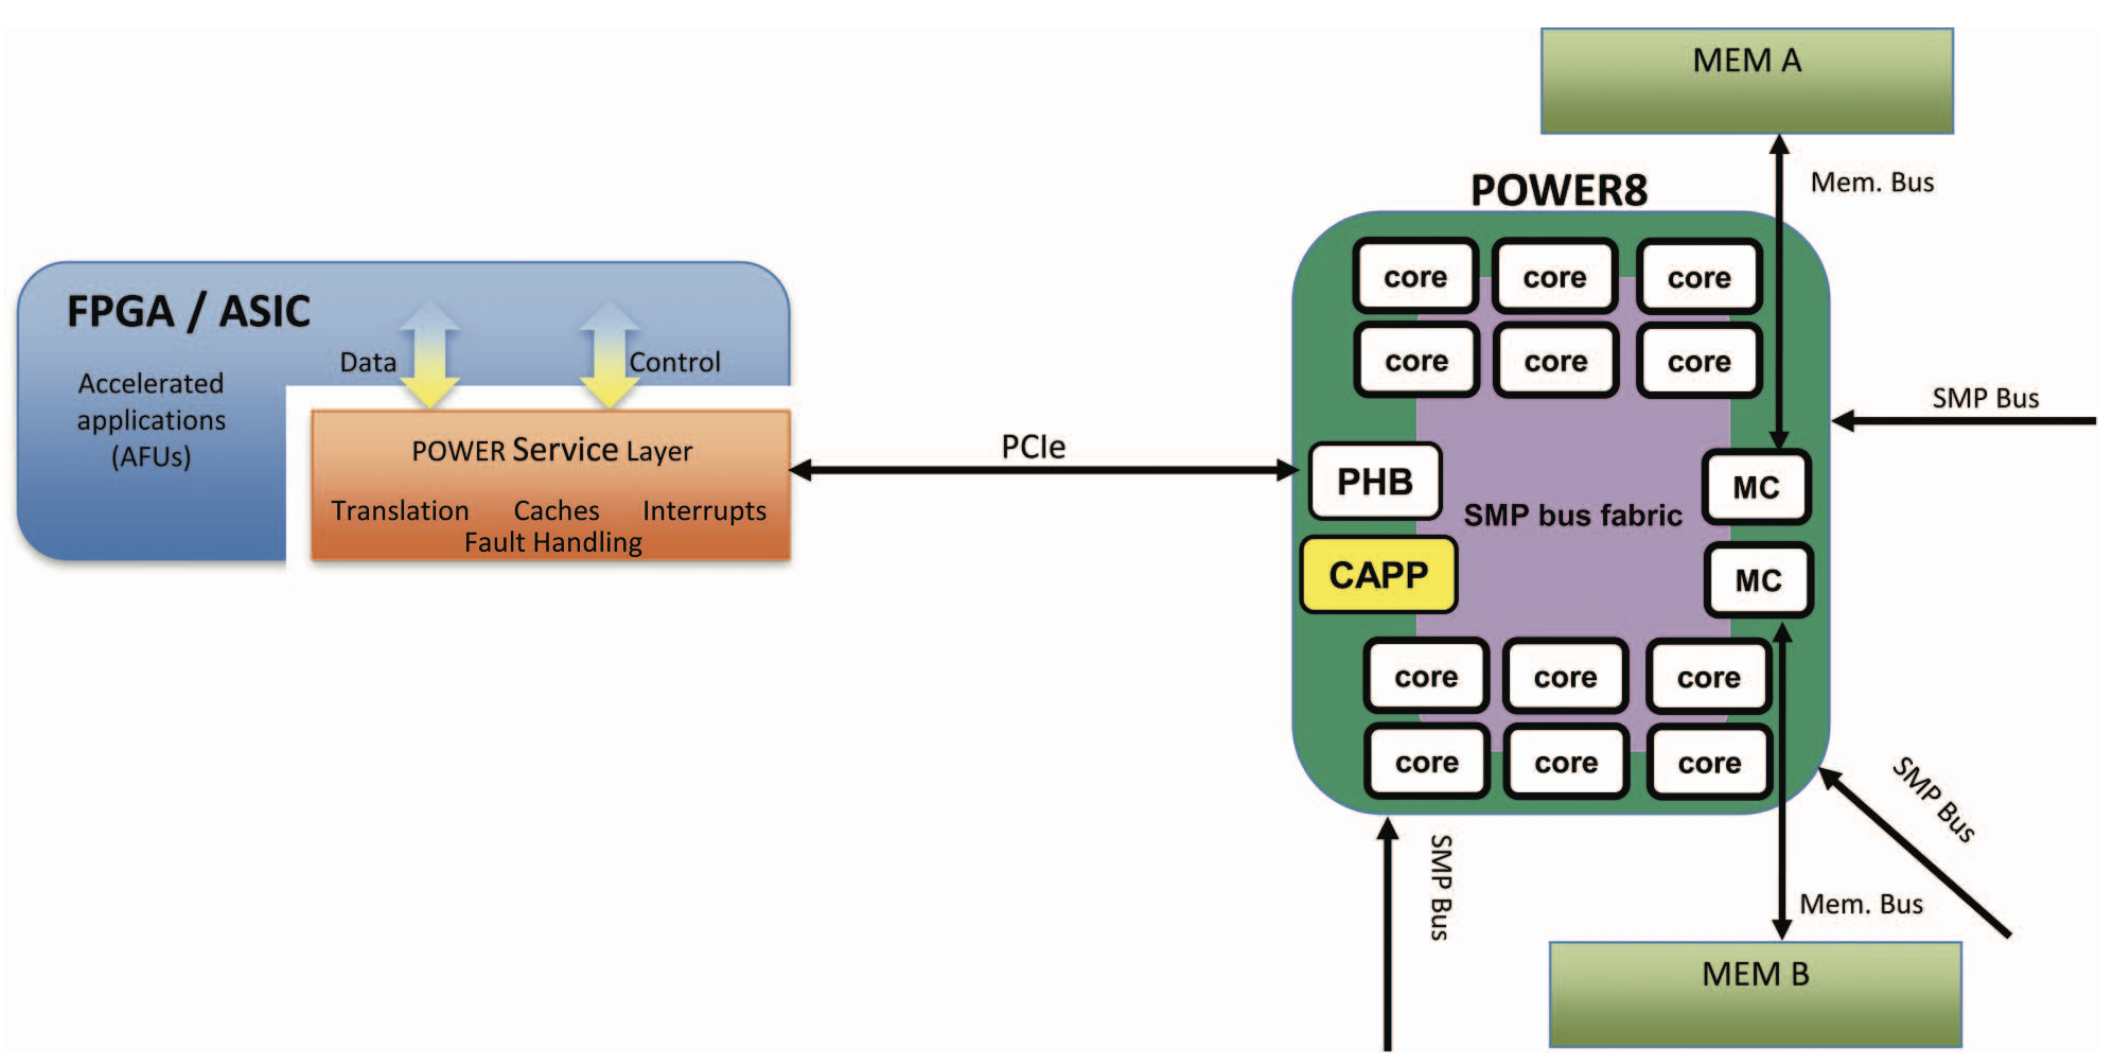
\includegraphics[width=0.85\textwidth]{3-capi.png}
  \caption{System architecture of a CAPI attached device \cite{capi_ibm}.}
  \label{fig:3-capi}
\end{figure}

When the CAPP, PHB, PCI Express and PSL are combined, the AFU is able to operate coherently on data in host memory. To reference the requested memory, the AFU uses effective addresses that are translated by a memory management unit (MMU) within the PSL. The PSL may also send interrupts to the host processor on AFU completion or to indicate a translation fault.\\
The interface provided by the PSL to the AFU hides cache coherence complexities and address translation. AFUs request host memory using a load-store model to user space effective addresses. Requests can be either cacheable or write-through (not cached). Cacheable requests are typically used to communicate control information between multiple processes and can be stored within a \SI{256}{\kilo\byte} cache within the PSL \cite{capi-white}. Write-through requests are typically used for data manipulation outside of the coherence domain and therefore require less messages to be transmitted over the PCI Express link and reduce overhead.\\
The programming model requires the application to setup data for the attached device in host memory, and to notify the AFU when the data is ready to be consumed. It is not possible to transfer data from the host processor to the AFU directly because the AFU has to master read and write commands for data located in host memory \cite{capi-bw}. The AFU can be notified in two different ways, either the AFU polls a location in host memory or the application running on the host writes into a specific MMIO register on the attached device.



\subsubsection{Coherence}
Coherent host memory access is enabled by a combination of the CAPP and PSL and both contain cache lines used by the AFU. The CAPP acts as a proxy for the PSL and snoops coherence messages on the fabric. Snoops that hit cache lines present in the CAPP could generate messages, transmitted across the PCI Express link, for the PSL. Coherence enables an AFU to cache data from host memory and to request locks to implement atomic operations for example \cite{capi-manual}.



\subsubsection{Address Translation}
In order for the AFU to operate on effective addresses, the PSL consists of an MMU that uses the host processor's page tables \cite{capi-zurich}. This enables AFUs to de-reference pointers, similar to a thread running on the host processor. System software manages page faults \cite{capi-white}. The MMU performs address translations and caches recent translations, in order to avoid page table walks. The CAPP also snoops translation invalidation messages from the fabric since the PSL consists of a translation cache.

%\todo{
%- Yvo: Subho, you mentioned that you had used CAPI and found that the locks present in the protocol where rather slow, or something along those lines. For my master thesis, I am looking into OpenCAPI, which uses atomics instead. I was wondering if you could provide me with more information about why the locks in CAPI where not as fast as desired and how you worked with this.
%Subho: I dont think the performance is a problem. The problem is that if you use the C++11 or POSIX locks in the software side, it is not quite clear how the locking protocol is implemented. So when we try to implement the the CAPI side of things, it becomes difficult to first understand the LINUX implementation and then figure out how to do something similar in hardware.
%In any case, high contention locks are a really bad. As FPGA very rarely gets the lock since it is much slower. I would advise using test and test and set based protocols along with priority to reverse the effects from the slow clock speeds in the FPGA.
%- Lance Thompson slides OpenCL CAPI: CAPI is shared virtual memory. Shared buffers can directly be instantiated instead of issuing memcpy functions.\\
%- great slides on PCIe versus CAPI from: Enabling Coherent FPGA Acceleration - Allan Cantle\\
%- has cache coherency\\
%- basically, WED concept exists in CAPI 1 (see CAPI UG), but no specifics regarding how this struct looks are defined.\\
%}

%\todo{CAPI interface summary from \url{https://www.xilinx.com/support/documentation/application_notes/xapp1293-amba-axi4-to-ibm-capi-adapter.pdf}\\
%The power service layer (PSL), is used by the accelerator to interface with the POWER8 system. It offers cache-line oriented services to an accelerator by way of five independent interfaces:
%- Control interface: The interface that allows the main application on the host to start, stop or reset the accelerator.
%- Command interface: The interface that is used by the accelerator to send read/write host memory requests.
%- Response interface: The interface that is used to acknowledge the accelerator about the completed commands.
%- Write buffer and read buffer interface: The interface that is used by the accelerator to send and receive data to, or from, the host memory.
%- MMIO interface: The interface that is used by the main application on the host to access the registers within the accelerator.

%There is a READY/VALID handshake in the PSL for flow control support. The data/responses are not always returned to the accelerator in the same order as the commands are issued.
%}

%\todo{From \url{http://events.linuxfoundation.org/sites/events/files/slides/lcjp15_mackerras.pdf}\\
%Two types of AFU for CAPI:
%“Dedicated” AFU can only be used by a single application
%“Directed” AFU supports multiple contexts and can be used by several applications concurrently
%}



\subsection{CAPI 1.0}
\label{sec:capi-1.0}
The first generation of CAPI was introduced with the IBM POWER8 processor in 2014 \cite{capi-white}. Since there is only one CAPP unit per POWER8 processor, the number of attached CAPI 1.0 devices is limited by the number of processors in the system. To improve adoption, Xilinx released an AXI4 to CAPI 1.0 adapter \cite{xilinx-xapp1293}.\\
The total bandwidth available to a CAPI 1.0 attached device is determined by the underlying PCI Express Gen 3 interconnect and the number of lanes. CAPI 1.0 supports eight or sixteen lanes per attached device \cite{opencapi-enablement}. The online CAPI Developers Community used a Nallatech P385-A7 FPGA attached using an eight lane PCI Express Gen 3 interface in conjunction with a POWER8 S824 system to assess the bandwidth and latency of CAPI 1.0 \cite{capi-bw}. The measurements were obtained using a modified \textit{memcpy} demo supplied with the developer kit. When data resides in host memory, a read bandwidth of \SI{3.42}{\giga\byte\per\second} was achieved with an average latency from PSL request to response of \SI{864}{\nano\second}. Similarly, write bandwidth of \SI{3.88}{\giga\byte\per\second} with an average latency of \SI{838}{\nano\second} was achieved. Reads and writes that hit in the PSL cache achieved a latency of \SI{120}{\nano\second}.\\
Due to the protocol overhead of CAPI 1.0 on top of PCI Express Gen 3, the obtained bandwidth is significantly less compared to the theoretical capabilities of PCI Express Gen 3. On the flipside, CAPI 1.0 provides several features and usage models that are not possible with a traditional PCI Express Gen 3 interconnect.

%The datasheet of the FPGA \cite{nalla-fpga} used states that the device is tested at PCI Express Gen 3 speeds, but by default operates at Gen 2 speeds. The simplex bandwidth for Gen 2 is \SI{4.0}{\giga\byte\per\second}. This explains the relatively low bandwidth obtained in comparison to the expected bandwidth for eight lanes of PCI Express Gen 3.

%\todo{
%- If PCIe Gen 3 has atomic op extension (partly proposed by IBM), why weren't they used for CAPI? Intel supports it since from Haswell (2013).\\
%}



\subsubsection{Streaming Framework}
The Streaming Framework is an extension to CAPI 1.0, designed and implemented by Matthijs Brobbel \cite{brobbel-github}. Instead of presenting the PSL interface to an AFU designer, a simple read and write streaming interface is presented with cache line granularity (128 bytes), similar to a DMA. It supports a single stream (multiple streams in simulation only) and returns read data in order, whereas the underlying CAPI interface does not guarantee such ordering. The philosophy behind the Streaming Framework is to hide the hassle of directly talking to CAPI by simplifying the interface. Preliminary results of a \textit{memcpy} AFU show a bandwidth of nearly \SI{3.3}{\giga\byte\per\second} using a Nallatech P385-A7 FPGA card with eight PCI Express Gen 3 lanes \cite{brobbel-slides}. Similar to the explanation in Section \ref{sec:capi-1.0}, the CAPI 1.0 protocol overhead on top of PCI Express Gen 3 limits bandwidth.

%the FPGA card used operates at PCI Express Gen 2 bandwidth.



\subsubsection{Storage, Networking, and Analytics Programming}
The Storage, Networking, and Analytics Programming (SNAP) framework enables designers to easily integrate FPGA-based accelerators to work with data located in host memory, flash or attached storage, or from other connected devices such as Ethernet \cite{snap-slides}. One could argue whether it is a continuation of the Streaming Framework in the sense that a simplified interface eases integration. SNAP consists of an AXI-to-CAPI bridge, MMIO registers, a host DMA, and a job management unit \cite{snap-github}.\\
An AFU can be controlled using an AXI-lite interface and the AFU has access to host memory through a coherent 512 bits wide AXI interface operating at \SI{250}{\mega\hertz} \cite{fuchs}. Additionally, AXI bridges to DRAM and NVMe are available. All of these hardware units are accompanied by a software library. No bandwidth results are public yet, but SNAP ought to be able to achieve the same bandwidth as CAPI 1.0.



%\todo{SNAP\\
%- Yvo: Is SNAP stream or load-store based? If it is stream based, what is the maximum number of streams supported?
%Bruce: SNAP can be both a flow-through model or an off-load model. But to be sure we are talking about the same thing, let me attach a few slides. Slide 1 is what I think of when you say stream vs. load-store, where the first picture (labeled "off-load" is the load-store model). The 2nd and 3rd slides are two different modes that SNAP can do (See attached file: SNAP Slides.pptx).\\
%}

%\todo{
%- there are other frameworks which try to make hardware acceleration easier as well. there is a recent initiative called the vineyard \url{http://vineyard-h2020.eu/en/news-events.html}, i also found a paper about it. but other than that there are not really any frameworks. only for specific accelerators such as intel quickassist technology \url{https://01.org/sites/default/files/page/332125_002_0.pdf} and amd. they are called in-socket accelerators (ISAs) \url{https://www.hpcwire.com/2009/01/06/a_framework_for_interfacing_configurable_hardware_accelerators/}. then there are frameworks specific to gpus, such as cuda and amd ROCm. we also have openCL, works as following with fpga \url{https://streamhpc.com/blog/2014-09-16/use-opencl-fpgas/}. opencl just converts code to HDL. i believe there is also something like Go to HDL (in snap?). still snap offers much more, more like a full framework for multi-context hetereogenous fpga acceleration. should find an official description of what the goal of SNAP is. probably can be found within the official slides i have about snap. xilinx also has a tool to go from a higher level language to HDL. then there is haskell to hdl. but this is probabl too far off topic\\
%- intel proposes opencl programmable fpga with xeon using opencl
%}


\subsection{CAPI 2.0}
The successor to CAPI 1.0 can be found in the IBM POWER9 processor \cite{stuecheli-power9}. Features from CAPI 1.0 are retained and the main improvement is the use of PCI Express Gen 4 that doubles the available bandwidth per lane. The effective bandwidth, compared to CAPI 1.0, will be more than double because protocol overhead is reduced by including packets with a larger payload. Another improvement is the addition of a host thread wake-up construct in hardware \cite{opencapi-enablement}.





\section{OpenCAPI}
OpenCAPI is a continuation of CAPI, but an open standard, that allows a microprocessor, agnostic to processor architecture, to attach to coherent user-level devices and advanced memories \cite{stuecheli-power9}. It provides a high-bandwidth, low latency interface optimized for ease of programmability and integration. By implementing complexities of coherence and virtual addressing on the host microprocessor, attached devices can be simplified and are interoperable across multiple processor architectures. Attached devices operate natively within an application’s user space and coherently with processors, since it appears as a peer to the host processor cores by sharing the same virtual memory space. This allows an attached device to fully participate in an application running on a host processor without kernel and device driver overhead of data copies or pinned pages and simplifies the programming model. Besides accelerators, OpenCAPI also supports classic and emerging memory and storage technologies. Chapter \ref{sec:ch2} discusses OpenCAPI 3.0 in much more detail.

%\todo{
%- WED removal: "For OCAPI this was one thing the hypervisor wanted removed. They felt this should be left up to an AFU and application and not part of the architecture. -Curt".\\
%- Google's TPU2 deep learning chip uses the BlueLink 25G connector according to this article \url{https://www.nextplatform.com/2017/05/22/hood-googles-tpu2-machine-learning-clusters/}. Not many details have been released up until now, check out when writing thesis if there is a paper or something like that talking about the TPU2 and BlueLink 25G.\\
%- compare PCIe versus OCAPI latency and cite Joerg. Note that latency is close to DRAM latency.\\
%}



\subsection{Architecture}
In essence, OpenCAPI uses the philosophy behind CAPI and replaces the underlying PCI Express based protocol with a streamlined point-to-point standard designed from scratch \cite{opencapi-enablement, benton, opencapi-jeff-preso}. With CAPI, address translation was done on the attached device in the PSL. In OpenCAPI, the virtual-to-physical address translation occurs in the host processor and enables a shared virtual address space. By pushing the translation hardware into the host silicon, the protocol layers are asymmetric on the host and attached device, and the data link and transaction layers are very thin on the attached device. This reduces design complexity and is especially beneficial for FPGAs since less resources are spent on the interconnect and more can be used for the actual accelerator. Initially, OpenCAPI will not support a coherent cache on the attached device, contrary to CAPI. Nonetheless, coherent memory accesses between the host and attached device are supported.\\
Attached devices never have access to physical addresses due to the shared virtual memory space. This improves security by eliminating the possibility of a defective or malicious device accessing memory locations belonging to the kernel or other applications that it is not authorized to access. Also pointers can be dereferenced on the attached device. This enables memory access patterns such as pointer chasing and linked lists without driver involvement. Multiple contexts are supported within the protocol, allowing multiple threads to utilize the attached device simultaneously. To synchronize threads and facilitate multi-thread programming, atomic memory operations are supported. In addition, special opcodes are available for warming up the address translation cache in the host. Finally, in order to reduce translation latency when using a new page, a new mechanism for waking up a host thread with low latency instead of interrupts or polling of host memory.
%One might argue that losing cache coherence is not a big problem due to the low latency atomic operations available. Also the WED paradigm is not present in OpenCAPI. Due to the open nature of the consortium, the paradigm used should be more general and the implementation left to the device designer, according to feedback IBM received from CAPI customers REF Curt. Also because memory and storage devices are part of the OpenCAPI use cases.



\subsection{OpenCAPI 3.0}
The first processor to use OpenCAPI is the IBM POWER9. Since it is a continuation of CAPI, the first generation of the OpenCAPI standard is called OpenCAPI 3.0. It will share the BlueLink 25G I/O facility with NVLink 2.0, peaking at a half-duplex bandwidth of \SI{25}{\giga\bit\per\second} at eight lanes per attached device. More information regarding the POWER9 processor and OpenCAPI 3.0 can be found in Chapter \ref{sec:ch2}.\\
The most recent source as of writing this thesis is a slide deck to inform on the progress of OpenCAPI 3.0 presented at the end of 2017. A POWER9 processor was paired with an Alpha Data 9V3 FPGA card with a Xilinx VU3P FPGA and achieved a bandwidth of roughly \SI{22}{\giga\byte\per\second} for streaming read and write operations \cite{opencapi-enablement}.\\
Throughout this thesis, OpenCAPI will be used as a proxy for OpenCAPI 3.0, unless specifically stated otherwise.

%\todo{
%- Enablement slides: "Latency measurements can be obtained under NDA with partner"\\
%}



\subsection{OpenCAPI 4.0}
%\todo{- What does rollover to interrupt mean?}

OpenCAPI 4.0 will continue where 3.0 left off and is still in definition. One of the main features is the re-introduction of cache coherency on the attached device. This provides a latency advantage for frequently used data. This cache will use effective addresses while CAPI uses real addresses \cite{opencapi-enablement}. Address translation will occur on the host similarly to OpenCAPI 3.0.\\
New features consist of additional link widths of four, sixteen and 32 lanes compared to a single link configuration of eight lanes for OpenCAPI 3.0 \cite{opencapi-forum}. The low latency communication mechanism (wake host thread) between the attached device and host application as is present in OpenCAPI 3.0 will be enhanced by rollover to interrupt. This avoids the use of current inefficient mechanisms such as interrupts or polling of the host memory

%\subsection{Intel QPI / UPI}
%\todo{- Peter: talk about this at all?\\
%- Is coherent protocol, mostly used for connecting multiple sockets, but also FPGAs and ASICs can be attached, although less popular. \url{https://www.intel.it/content/dam/doc/white-paper/quick-path-interconnect-introduction-paper.pdf}\\
%- About FPGA/ASIC: \url{http://www.ece.cmu.edu/~calcm/carl/lib/exe/fetch.php?media=carl2012_oliver_slides.pdf}\\
%}





\section{CCIX}
Similar to OpenCAPI, CCIX is an initiative promoted by several companies for an open interconnect standard that is host architecture agnostic \cite{ccix-website}. CCIX extends the processor's coherency domain to heterogeneous devices such as accelerators, network adapters, and memory and storage solutions. This is done using a driver- and interrupt-free framework for data sharing across the link in hardware and allows low-latency main memory expansion as well.

\subsection{Architecture}
CCIX is an extension to PCI Express. Therefore, little to no modification to PCI Express controllers is required. It uses the PCI Express extension for address translation services via ATS/PRI \cite{benton} and requires additional logic, as shown in \autoref{fig:3-ccix}, to implement the CCIX transaction layer. This layer carries the coherence messages, while the CCIX protocol layer and link layer implement the coherence protocol and act upon it. These blocks require tight integration with internal system-on-chip (SoC) logic for caching, and depend on the SoC’s ISA. SoC designers implementing CCIX typically partition the CCIX protocol and link layers from the CCIX transaction layer, so they can achieve tight integration with the internal SoC logic \cite{using-ccix}.

\begin{figure}[H]
  \centering
  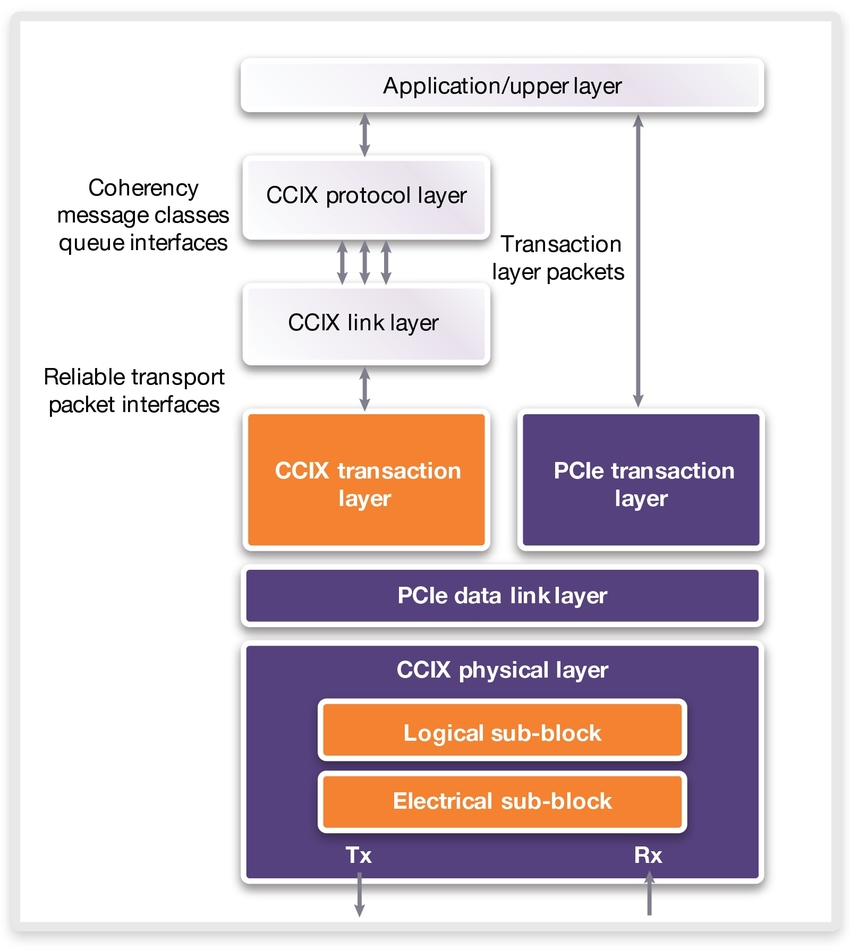
\includegraphics[width=0.50\textwidth]{3-ccix.jpg}
  \caption{Layering diagram of the CCIX standard \cite{using-ccix}.}
  \label{fig:3-ccix}
\end{figure}

The standard supports peer-to-peer and switched topologies with unidirectional bandwidths between \SI{1}{\giga\bit\per\second} and \SI{3.125}{\giga\bit\per\second} per lane. Links consist of eight or sixteen lanes. It provides full cache coherence between the processor and accelerators. Communication with CCIX-attached devices is managed by vendor-specific drivers and libraries.\\
During the typical PCI Express initialization process, the highest mutually supported transfer speed is determined between the two CCIX components. Software running on the host checks configuration registers on the attached device to decide on the transfer speed.





\section{AMBA AXI}
The Advanced Microcontroller Bus Architecture (AMBA) is an open standard by ARM for interconnect protocols. Today, protocols from AMBA are the \textit{de facto} standard in the world of ASICs, FPGAs, SoCs and embedded devices for communication between cores and between cores and attached devices. Currently, FPGAs mostly use the Advanced eXtensible Interface (AXI) protocol by AMBA that will be discussed in this section.



\subsection{Architecture}
While AMBA owns multiple interconnect standards, AXI is the most widely used standard in the world of FPGAs. An example is the abundant use of it in the Xilinx FPGA tool chain and all hardware modules available in the SNAP framework. The latest generation of AXI was released in 2010 in the fourth iteration of the AMBA specification \cite{amba4}.\\
AXI targets high performance and high clock frequency systems by providing a memory-mapped interface that consists of five independent channels: read address, read data, write address, write data, and write response. AXI does not define a specific clock frequency or data width in order to serve the needs for multiple requirements. As an example, the Xilinx AXI generated modules can be configured with a data width of up to 1024 bits \cite{xilinx-pg059}. The frequency depends on the FPGA used in this case and could be in the order of \SI{250}{\mega\hertz} \cite{fuchs}.



\subsection{Handshake Protocol}
The simple uni-directional protocol employs a ready-valid handshake to support flow control in both directions \cite{xilinx-xapp1293}. In essence, the master provides data with an associated valid signal and the slave indicates when it is ready by asserting a ready signal. When at a rising clock edge both valid and ready signals are asserted, data is transferred and both signals are deasserted again.

    

\subsection{AXI Protocol Derivatives}
AXI allows for bursts of data of up to 256 transfer cycles with a single address phase. A derivative is the AXI-Lite standard that is mostly used for low-throughput memory-mapped data transfers. In comparison to AXI, it does not support burst transfers but instead only the transfer of an address-data pair. Another derivative is AXI-Stream, used specifically for streaming applications. The complex address channels are removed and only the ready-valid handshake signals are left. This results in the simplest interface within the AXI family.



\subsection{AXI Coherence Extension}
The AXI Coherence Extension (ACE) \cite{amba4} is an extension to the fourth iteration AMBA specification introduced in 2011. ACE introduces additional signals to enable system-wide coherence \cite{axi-coherence}.\\
The introduction of ACE enabled heterogeneous SoCs such as the ARM big.LITTLE architecture. A derivative of ACE called ACE-Lite enables IO coherency in the sense that an attached device can read from the cache present in the ACE-capable host processor.

%\todo{
%- info on ACE = AXI coherence extension. Problem is that for example hard interconnect IP can be supplied, like CCI-400, with a predefined set of ports. That means little flexibility.\\
%}



%\subsection{CHI}
%\todo{
%- recently announced AMBA5 CHI \url{https://www.arm.com/about/newsroom/arm-announces-amba-5-chi-specification-to-enable-high-performance-highly-scalable-system-on-chip.php} and AHB standards. I downloaded both standards.\\
%}



%\todo{\url{https://community.arm.com/processors/f/discussions/6666/why-is-there-an-acp-interface-for-many-arm-processors}\\
%What is ACP?

%Most of ARM's MPCore processors include an ACP, or Accelerator Coherency Port.  ACPs are just AXI slave ports.  You can connect an AXI master to the port, and the transactions generated by that master will pass through the MPCore processor in order to reach the main memory system.

%Why?

%This is a way of taking a non-cache coherent master and making it cache coherent.

%As the master's transactions pass through the processor, they are visible to the coherency logic in the processor.  This means that should they access an address held in the processor's caches, it can take the necessary steps to ensure coherency. Exactly how this works is down to the specific MPCore processor.

%Note: In practice, it would have to be a non-cached master.  As the ACP only gives visibility of the bus transactions, not any up-stream caches.

%Who initiates transactions over ACP?
%The master (the thing you connected to the ACP). From its perspective not much has changed.

%Check link for more information.
%}




\newpage
\section{Interconnect Comparison}
The preceding sections provided information about the state-of-the-art interconnects. This section summarizes their main characteristics and compares them to the desired requirements for future interconnects discussed in Section \ref{sec:trends-interconnect}.



\subsection{Bandwidth and Latency}
In order to compare various interconnect standards in more detail, the protocols involved and the system that is used should be investigated in more detail. Protocol overhead in transmitted data is for example not taken into account in the comparison presented in \autoref{tab:comparison}, nor are other factors such as packet overhead, and how acknowledge packets incluence bandwidth. System parameters can also affect performance such as payload size and the topology of the interconnect \cite{pcie-xilinx}. With a switched topology, packet congestion can occur if multiple endpoints make multiple requests simultaneously. Determining the latency has similar difficulties in that it depends on so many factors.\\
In general, there is a clear trend to increase the per lane transmission rate in order to provide for example enough bandwidth to accelerators for emerging workloads such as big data and machine learning.



\subsection{Address Space}
There is a trend towards a shared memory model and coherent interconnect with more bandwidth and lower latency. A shared address space across the host and attached devices simplifies the programming model and allows for new use cases.\\
Since PCI Express Gen 3, ATS is included in the specification and enables an ATC on attached devices. While this improves address translations, it does not share a translation table with the host processor as CAPI and OpenCAPI do. Therefore, emerging use cases are not yet possible on PCI Express nor on CCIX.



\subsection{Coherence}
Hardware-based coherence across host cores and attached devices should greatly simplify the programming model.\\
PCI Express uses a snoop filter to keep host caches coherent when host memory is accessed by the attached device. While this improves performance by decreasing data access latency, no coherent cache is present on the attached device itself. CAPI does support a coherent cache on the attached device at the cost of an increased protocol overhead. OpenCAPI will support this in the next generation as well, while currently only coherent memory access is provided. The additional protocol layers of CCIX enable cache coherency and the ACE extension works similarly for AXI interconnects.



\subsection{Synchronization}
With access to shared memory by the attached device, synchronization using shared variables between a thread running on the host and the attached device removes inefficiencies from using interrupts or communication using MMIO registers.\\
PCI Express supports three atomic operations to implement synchronization mechanisms, while CAPI only implements locks. OpenCAPI on the other hand supports multiple atomic operations with a ton of configuration possibilities per operation. This enables a wide variety of synchronization mechanisms to be implemented.

\begin{table}[H]
  \centering
  \caption{Comparison of state-of-the-art interconnect standards.}
  \label{tab:comparison}
  \begin{tabular}{ l | l | l | l | l }
    \textbf{Standard} & \textbf{Bandwidth} & \textbf{Address Space} & \textbf{Coherence} & \textbf{Synchronization} \\ \hline
    PCI Express Gen 3  & \SI{16.0}{\giga\byte\per\second}  & ATS     & Snoop   & Atomics \\
    PCI Express Gen 4  & \SI{32.0}{\giga\byte\per\second}  & ATS     & Snoop   & Atomics \\
    PCI Express Gen 5  & \SI{64.0}{\giga\byte\per\second}  & ATS     & Snoop   & Atomics \\
    CAPI 1.0    & \SI{16.0}{\giga\byte\per\second}  & Shared  & Cache   & Locks   \\
    CAPI 2.0    & \SI{32.0}{\giga\byte\per\second}  & Shared  & Cache   & Unknown \\
    OpenCAPI 3  & \SI{25.0}{\giga\byte\per\second}  & Shared  & Memory  & Atomics \\
    OpenCAPI 4  & \SI{100.0}{\giga\byte\per\second} & Shared  & Cache   & Atomics \\
    CCIX        & \SI{32.0}{\giga\byte\per\second}  & ATS     & Cache   & Unknown \\
    AXI\footnotemark & \SI{16.0}{\giga\byte\per\second} & Memory Mapped & Cache & Unknown \\
  \end{tabular}
\end{table}

\footnotetext{The bandwidth is calculated as the product of a 512 bit wide data bus operating at \SI{250}{\mega\hertz} as used by the SNAP framework \cite{fuchs}. However, higher bandwidths could be obtained by improving either or both parameters.}



\section{Preliminary Concluding Remarks}
\label{sec:3compare}
It is obvious that many advancements in interconnects have been made recently to bridge the gap between host processor cores and attached devices by tighter coupling and extending common concepts for homogeneous multi-core processors to attached devices.\\
Due to the desire of backwards compatibility, PCI Express is limited in terms of innovation and protocol changes. This resulted in a slow release of the Gen 4 specification. At the same time, multiple initiatives started to develop new interconnect standards such as CAPI, OpenCAPI, and CCIX.\\
Due to the support of higher signaling rates than PCI Express, shared memory with address translation and coherent host memory access, OpenCAPI 3.0 is of special interest during the remainder of this thesis. All of these features allow for new usage models and new workloads to be accelerated. In general, upcoming interconnect standards receive a significant increase in bandwidth and this impacts accelerator architectures and design choices.\\
The objective of the remainder of this thesis is to explore how multiple classes of accelerated workloads can be fed with the same or similar reconfigurable buffer architecture to improve designer adoption of OpenCAPI, or other high-bandwidth interconnects. In order to do so, Chapter 4 provides a deeper understanding of OpenCAPI.




%\todo{Interesting news links:\\
%\url{https://www.nextplatform.com/2017/06/30/infiniband-proprietary-networks-still-rule-real-hpc/}\\
%\url{https://www.nextplatform.com/2017/07/14/system-bottleneck-shifts-pci-express/}\\
%\url{https://www.nextplatform.com/2017/07/12/heart-amds-epyc-comeback-infinity-fabric/}\\

%- For comparison of IO on state of the art processor (Power9, etc) and future trends for the IO speeds\\
%\url{https://www.nextplatform.com/2017/07/10/ethernet-getting-back-moores-law-track/}\\
%}

  \chapter{OpenCAPI Characterization}
\label{sec:ch2}

%\todo{
%- Transferring 64B seems wasteful then. Therefore we work here on a cache line granularity.\\
%At tlx 64B data busses are provided. ocapi can transfer 64, 128 or 256B of data by taking multiple cycles over the data bus. power architecture cache line size is 128B. if 64B are requested, the CAPP unit in host cpu fetches the requested cache line of 128B and invalidates one half and transmits the other. transferring less than the cache line size seems wasteful. ask curt if it actually is. maybe in terms of control overhead? Also, do template overhead calculation. can we use all data flits in a single frame if data flits are 128B long?\\
%}

%\todo{MMIO:\\
%\url{https://en.wikipedia.org/wiki/Memory-mapped_I/O} \\
%Used by OpenCAPI. Complementary approach is port-mapped I/O (PMIO) and another option is using dedicated I/O processors. Memory-mapped I/O uses the same address space to address both memory and I/O devices. The memory and registers of the I/O devices are mapped to (associated with) address values. So when an address is accessed by the CPU, it may refer to a portion of physical RAM, but it can also refer to memory of the I/O device. Thus, the CPU instructions used to access the memory can also be used for accessing devices. Each I/O device monitors the CPU's address bus and responds to any CPU access of an address assigned to that device, connecting the data bus to the desired device's hardware register. To accommodate the I/O devices, areas of the addresses used by the CPU must be reserved for I/O and must not be available for normal physical memory. The reservation may be permanent or temporary.\\
%Another good source: \url{http://www.cs.uwm.edu/classes/cs315/Bacon/Lecture/HTML/ch14s03.html} \\
%A lab assignment with Verilog code: \url{http://web.eecs.umich.edu/~prabal/teaching/eecs373-f10/labs/lab3/}\\

%\url{https://en.wikipedia.org/wiki/Address_bus} \\
%"A system with a 32-bit address bus can address $2^{32}$ (4,294,967,296) memory locations."

%Example from the MMIO wiki page:\\
%8-bit processor with 16-bit address lines. 16-bit address line results in 65536 memory locations.
%\begin{equation}
%  $16~bits = 2^{16} = 65536 = 64~kibibytes = 64*1024$
%\end{equation}
%On such a system, the first 32 KiB of address space may be allotted to random access memory (RAM), another 16 KiB to read only memory (ROM) and the remainder to a variety of other devices such as timers, counters, video display chips, sound generating devices, etc. The hardware of the system is arranged so that devices on the address bus will only respond to particular addresses which are intended for them, while all other addresses are ignored. This is the job of the address decoding circuitry, and that establishes the memory map of the system. This memory map contains gaps, which is also quite common in actual system architectures.}
%\todo{INTERRUPT: An interrupt is a signal to the processor emitted by hardware or software indicating an event that needs immediate attention. An interrupt alerts the processor to a high-priority condition requiring the interruption of the current code the processor is executing. The processor responds by suspending its current activities, saving its state, and executing a function called an interrupt handler (or an interrupt service routine, ISR) to deal with the event. This interruption is temporary, and, after the interrupt handler finishes, the processor resumes normal activities. There are two types of interrupts: hardware interrupts and software interrupts. Source: wikipedia}

To get a better understanding of the first OpenCAPI capable system, the system architecture of IBM's POWER9 processor is presented. While OpenCAPI is host architecture agnostic, the standard will be looked at in more detail with respect to the POWER architecture. Several supported accelerator paradigms are shown and finally two initial compatible Xilinx FPGAs are characterized.\\
While our research was being conducted, much of the information on OpenCAPI could only be obtained by talking to the right people, and we hope that this overview may prove useful to others who want to gain a better understanding of this interface.



\section{POWER9 System Overview}

%\todo{- P9 article \url{https://www.nextplatform.com/2017/12/05/power9-to-the-people/}\\
%- interesting about DDR: physically it can either read or write in one cycle. and there is some dead time between read and write because you have to 'turn the DDR around'. memory controller tries to hide this by reorganizing reads and writes. instead of r,w,r,w,etc you want for example r,r,w,w. in contrast, ibm buffer chip does have separate read and write channel. twice as much bw for read compared to write. maybe move this to bandwidth plots at system level.\\
%}

OpenCAPI \cite{opencapi-jeff-preso} is a successor to CAPI 1.0 \cite{capi_ibm} and enables direct attachment of any micro-architecture CPU to coherent user-level accelerators like ASICs and FPGAs and I/O devices such as network and storage controllers. The goal is to have a high-bandwidth and low latency interconnect optimised to enable streamlined implementation of attached devices. The first OpenCAPI enabled system will be in the upcoming POWER9 processor by IBM \cite{thompto-power9}.\\
\autoref{fig:2-p9-system} shows the system architecture of a superset of the various configurations. Depending on the model (SU or SO), there are up to 12 SMT8 or 24 SMT4 cores available accompanied by a collection of various on-chip accelerators such as gzip, 842 compression and AES/SHA cryptography engines. The memory controller supports either eight DDR4 channels or eight "Centaur" memory buffer chips that also act as an off-chip L4 cache. This yields sustained bandwidths of at least \SI{120}{\giga\byte\per\second} and \SI{230}{\giga\byte\per\second}, respectively.\\
POWER9 supports a wide collection of interconnect standards. In total, 48 PCIe Gen 4 lanes are available, which can also be used for CAPI 2.0, for a total half-duplex bandwidth of \SI{96}{\giga\byte\per\second}. Additionally, there are 48 BlueLink lanes operating at \SI{25}{\giga\bit\per\second} servicing either Nvidia NVLink 2.0 attached GPUs or OpenCAPI 3.0 attached devices. This enables an additional \SI{150}{\giga\byte\per\second} of half-duplex bandwidth. Other POWER9 sockets can be attached through an SMP interconnect, by using \SI{16}{\giga\bit\per\second} or \SI{25}{\giga\bit\per\second} lanes. Finally, the cache hierarchy and on-chip interconnect, called the fabric, ties all units together at a maximum bandwidth of \SI{7}{\tera\byte\per\second} \cite{stuecheli-power9}. Due to the coherent nature of the fabric, attached devices can seamlessly communicate with each other and system memory. What sets the POWER9 apart from other vendors is the extended coherency domain across processor cores and attached devices.

%\begin{figure}[H]
%  \centering
%  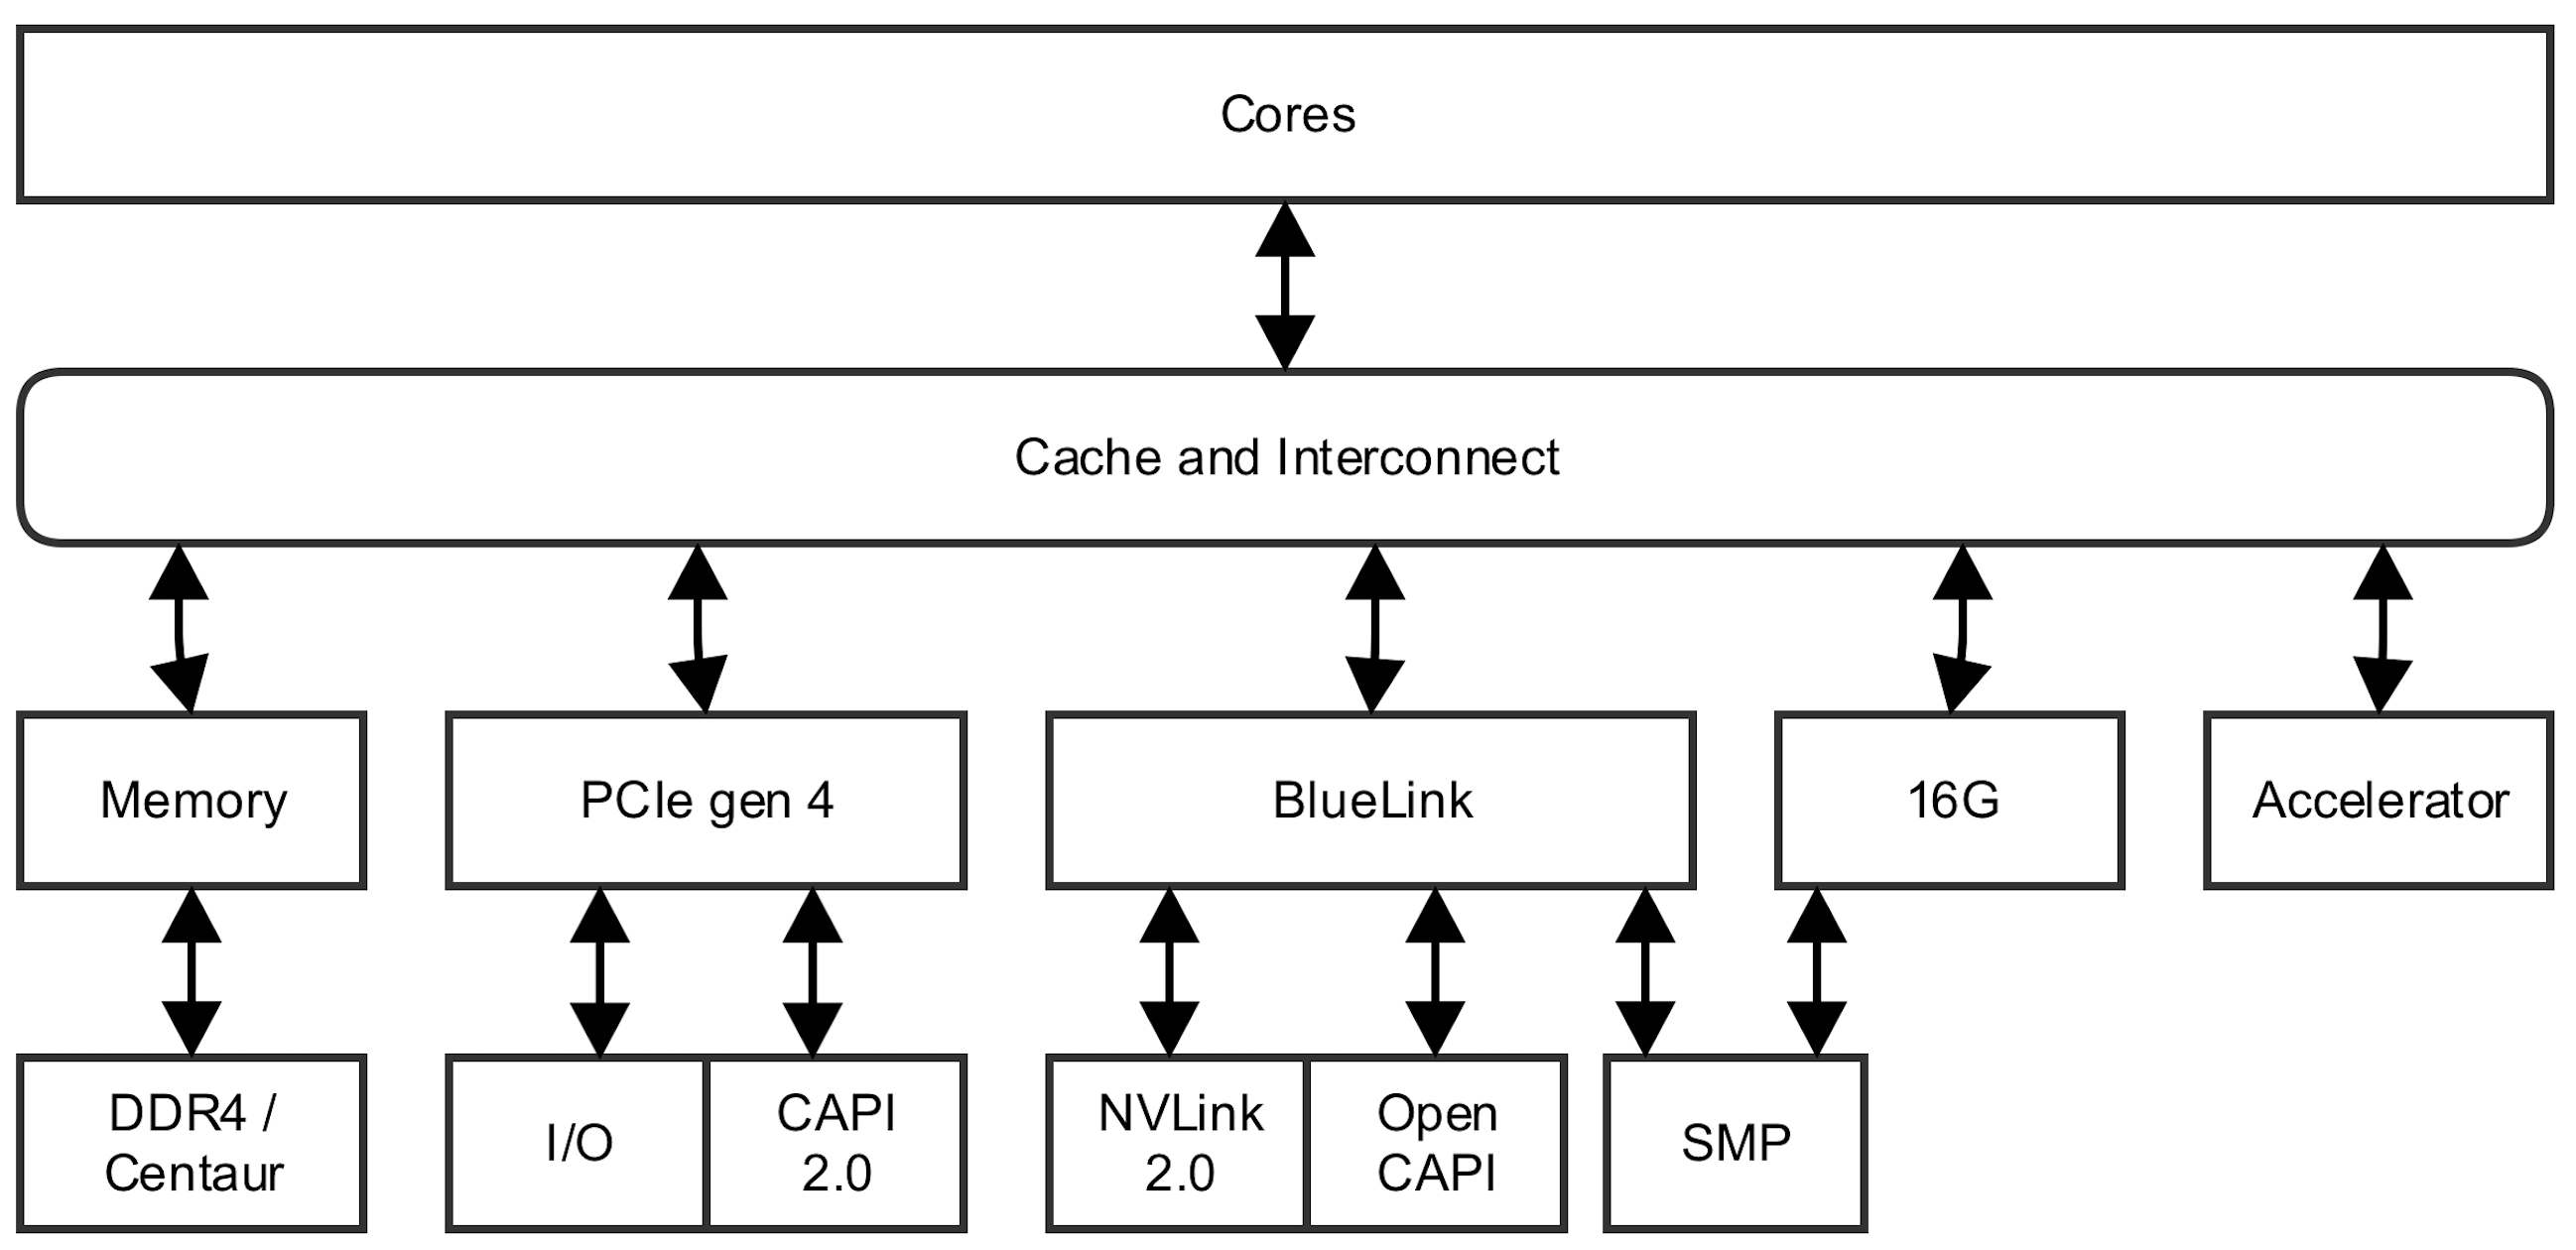
\includegraphics[width=0.80\textwidth]{2-p9-system.png}
%  \caption{System architecture of possible POWER9 configurations \cite{stuecheli-power9}.}
%  \label{fig:2-p9-system}
%\end{figure}
\begin{figure}[h]
  \centering
  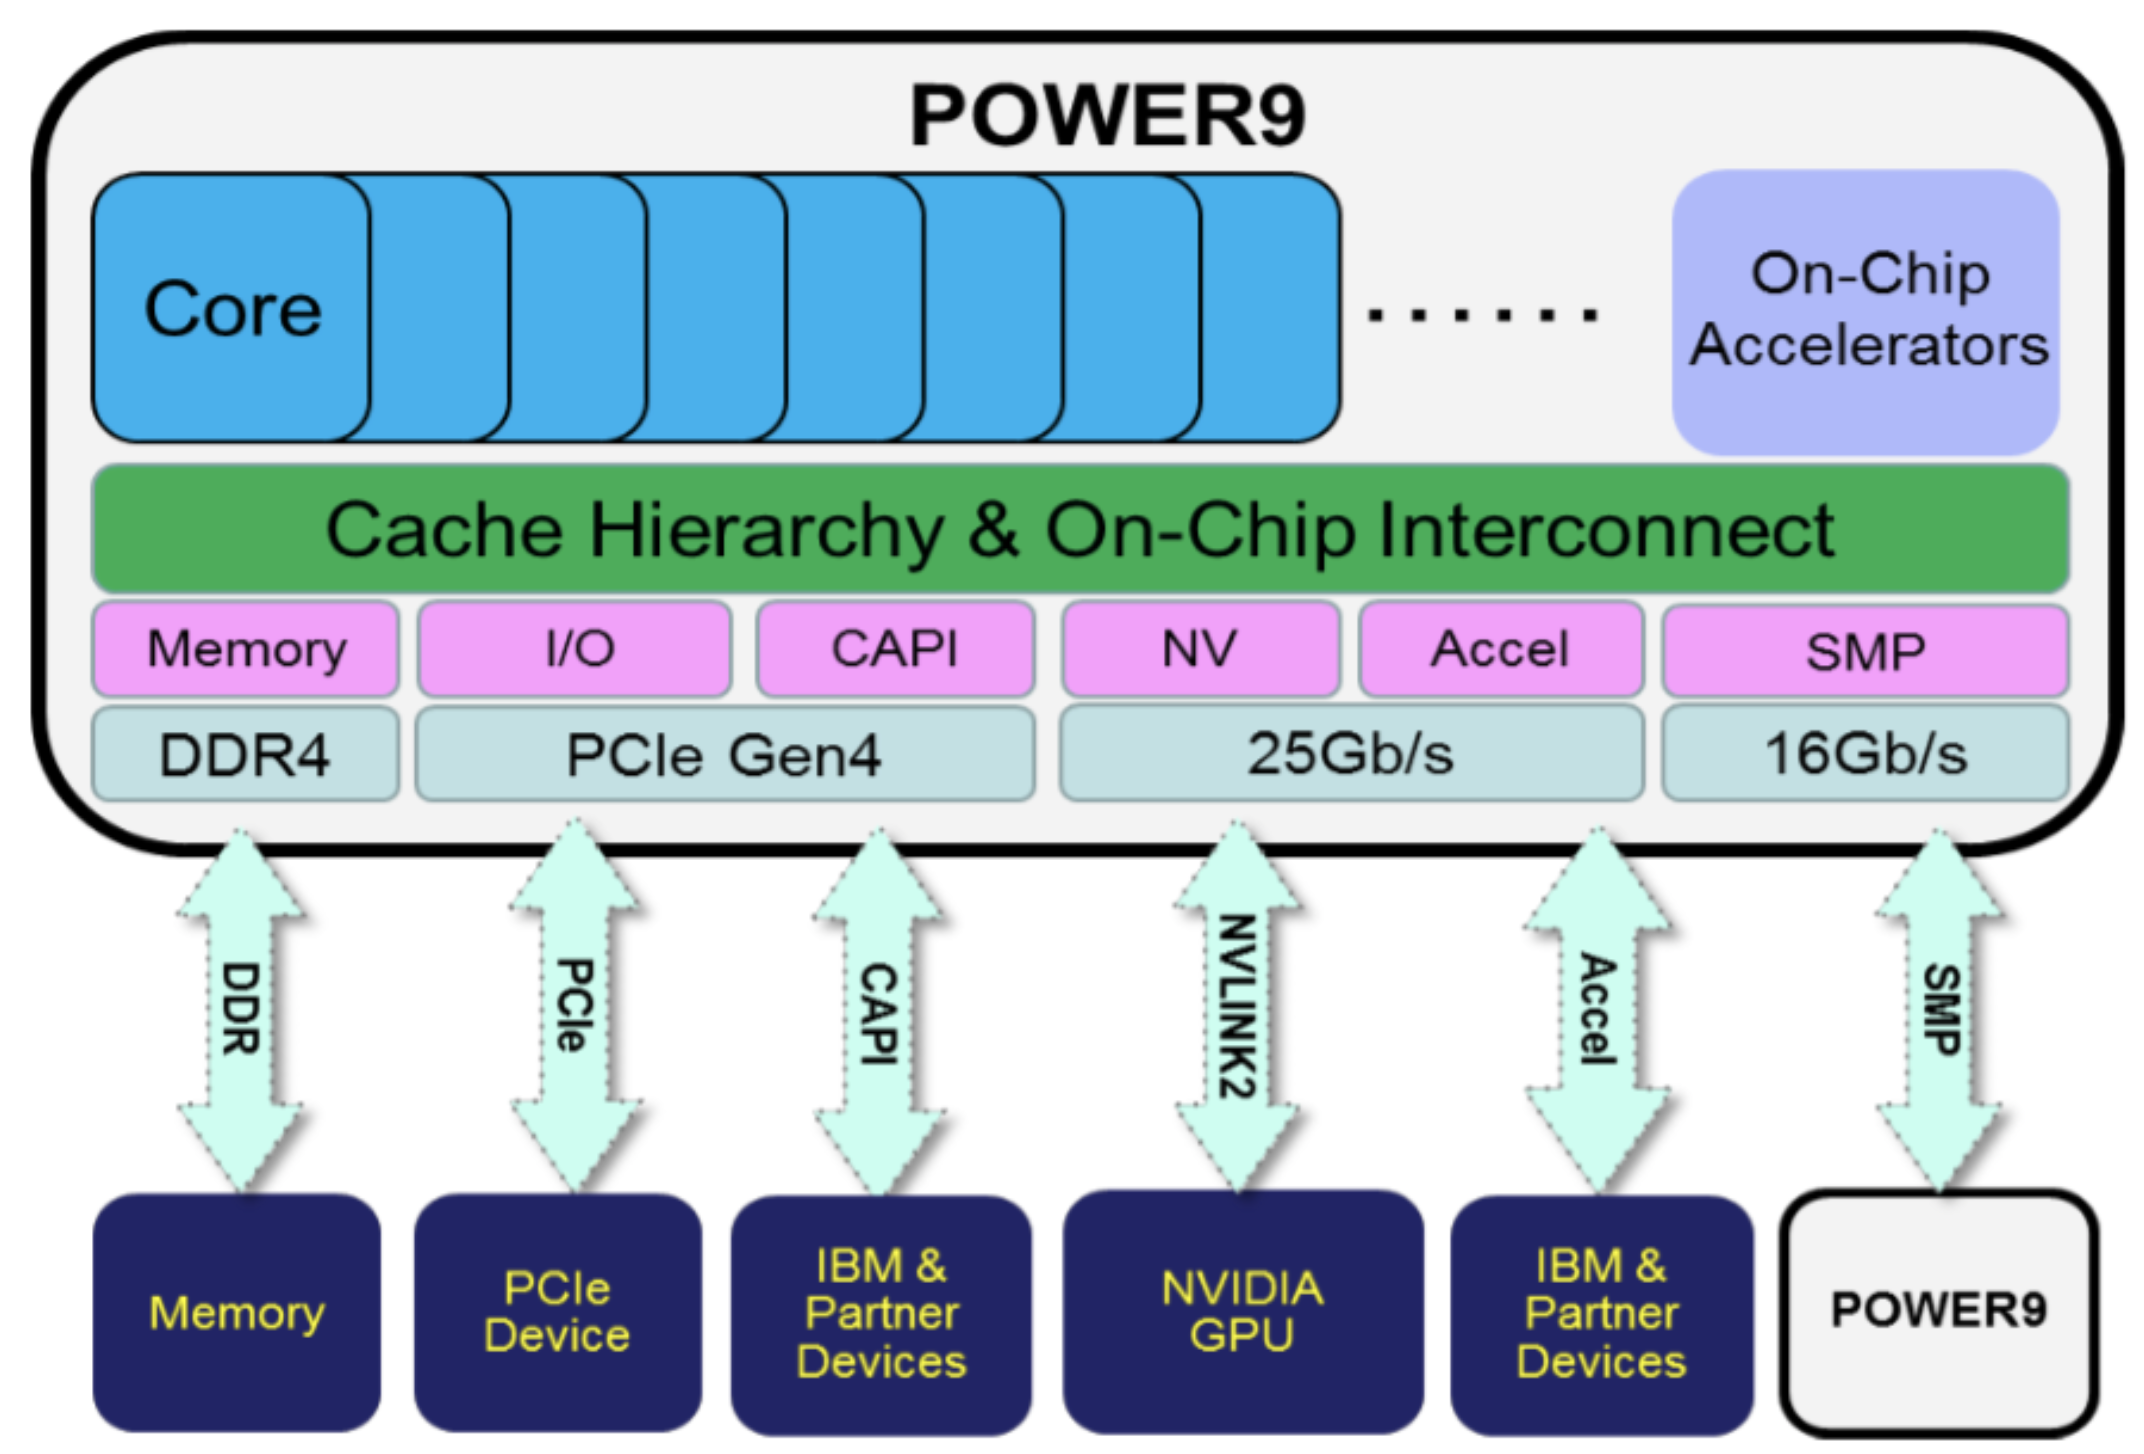
\includegraphics[width=0.70\textwidth]{2-p9-system-2.png}
  \caption{POWER9 system overview \cite{thompto-power9}.}
  \label{fig:2-p9-system}
\end{figure}





\section{OpenCAPI Architecture}
%\todo{- Curt: waiting on official P9 manual for the public.\\
%}

The OpenCAPI architecture consists of several protocol layers divided between the host and attached device \cite{ocapi-dl} \cite{ocapi-tl}. Logic is required on both sides to enable the protocol stack. All logic required for enablement on the host is called the Coherent Accelerator Processor Proxy (CAPP) and is architecture dependent. The CAPP for the POWER architecture is briefly mentioned, but our main focus is on the attached device side. While OpenCAPI also targets emerging storage class memory features, those will not be discussed further and are outside our scope.



\subsection{Protocol Stack}
\autoref{fig:2-ocapi-stack} shows the OpenCAPI stack that is partly located on the host CPU and partly on the attached device. OpenCAPI is a credit-based point-to-point protocol. The link has a number of credits that are consumed when data is transferred in order to throttle traffic. While in essence there are no differences from the point of view of the stack between attaching an ASIC or FPGA, only FPGAs will be considered due to the aim of the thesis.\\
In comparison to CAPI 1.0, the PSL is now located in the host processor, which removes the logic overhead within the FPGA. Complexities of coherence and virtual addressing are implemented on the host CPU to simplify the design of attached devices and facilitate interoperability across different CPU architectures. Due to the coherent nature, attached devices can operate natively within an application's user space. This allows attached devices to fully participate in an application without involvement or overhead of the kernel \cite{stuecheli-power9}.\\
The stack consists of several layers that are briefly introduced. Messages (packets) can be initiated by either the CAPP (host) or AP (AFU) and are called CAPP or AP command packets, respectively (see Section \ref{sec:packets}). When the Transaction Layer on either side receives a command packet, a response packet has to be sent back, called a CAPP or AP response packet, respectively. Note that while the stack looks symmetric, the transaction layers on both sides are very different, since their implementation depends on the host architecture and AFU protocol, respectively.

\begin{itemize}
  \item{\textbf{Host Protocol Layer} is the coherent connection to the rest of the host. The implementation is host architecture dependent and all required logic to implement OpenCAPI is called the CAPP (see Section \ref{sec:capp}).}
  \item{\textbf{Transaction Layer (TL)} converts host protocol-specific requests into CAPP command packets and generates and handles CAPP response packets. Internally it consists of a framer and parser.
  \begin{itemize}
    \item{\textbf{Framer} packetizes CAPP commands and responses along with credit packets into control flits according to various packing templates. Different templates exist since packets have different sizes. Control and data flits are sent to the DL while ensuring frame order.}
    % Flow control.
    % Error handling.
    % Manages virtual channels, virtual queues, and service queues associated with the virtual channels. Order is retained within virtual channels. See service queue and virtual queue in this glossary.
    \item{\textbf{Parser} receives DL frames consisting of control and data flits (see Section \ref{sec:frame}). It parses the control flit into AP command and response packets and returns credits to the Framer. The AP packets are passed to the host.}
  \end{itemize}
  }
  \item{\textbf{Data Link Layer (DL)} converts DL frames, consisting of a single control flit and between zero and eight data flits, to PHY transmittable data.}
  \item{\textbf{Physical Layer (PHY)} represents the actual connector and link on the host CPU. Each lane operates at \SI{25.78125}{\giga\hertz}. For the POWER9, each PHY brick consists of eight duplex lanes.}
\end{itemize}

In opposite order, the PHYX, DLX and TLX layers present on the FPGA act similarly to their host counterparts, where X stands for eXternal. However, the TLX does not handle responses. This has to be taken care of by the APL or AFU, depending on implementation.\\
An additional layer present on the FPGA is the AFU Protocol Layer (APL). This is an optional layer and an AFU can also directly interface with the TLX if desired. An example of this layer could be a bridge to AXI, the \textit{de facto} standard for FPGAs, similarly to the AXI4 to CAPI 1.0 adapter by Xilinx \cite{xilinx-xapp1293}. On the other side the APL interfaces with the Attached Functional Unit (AFU), or accelerator.

\begin{figure}[h]
  \centering
  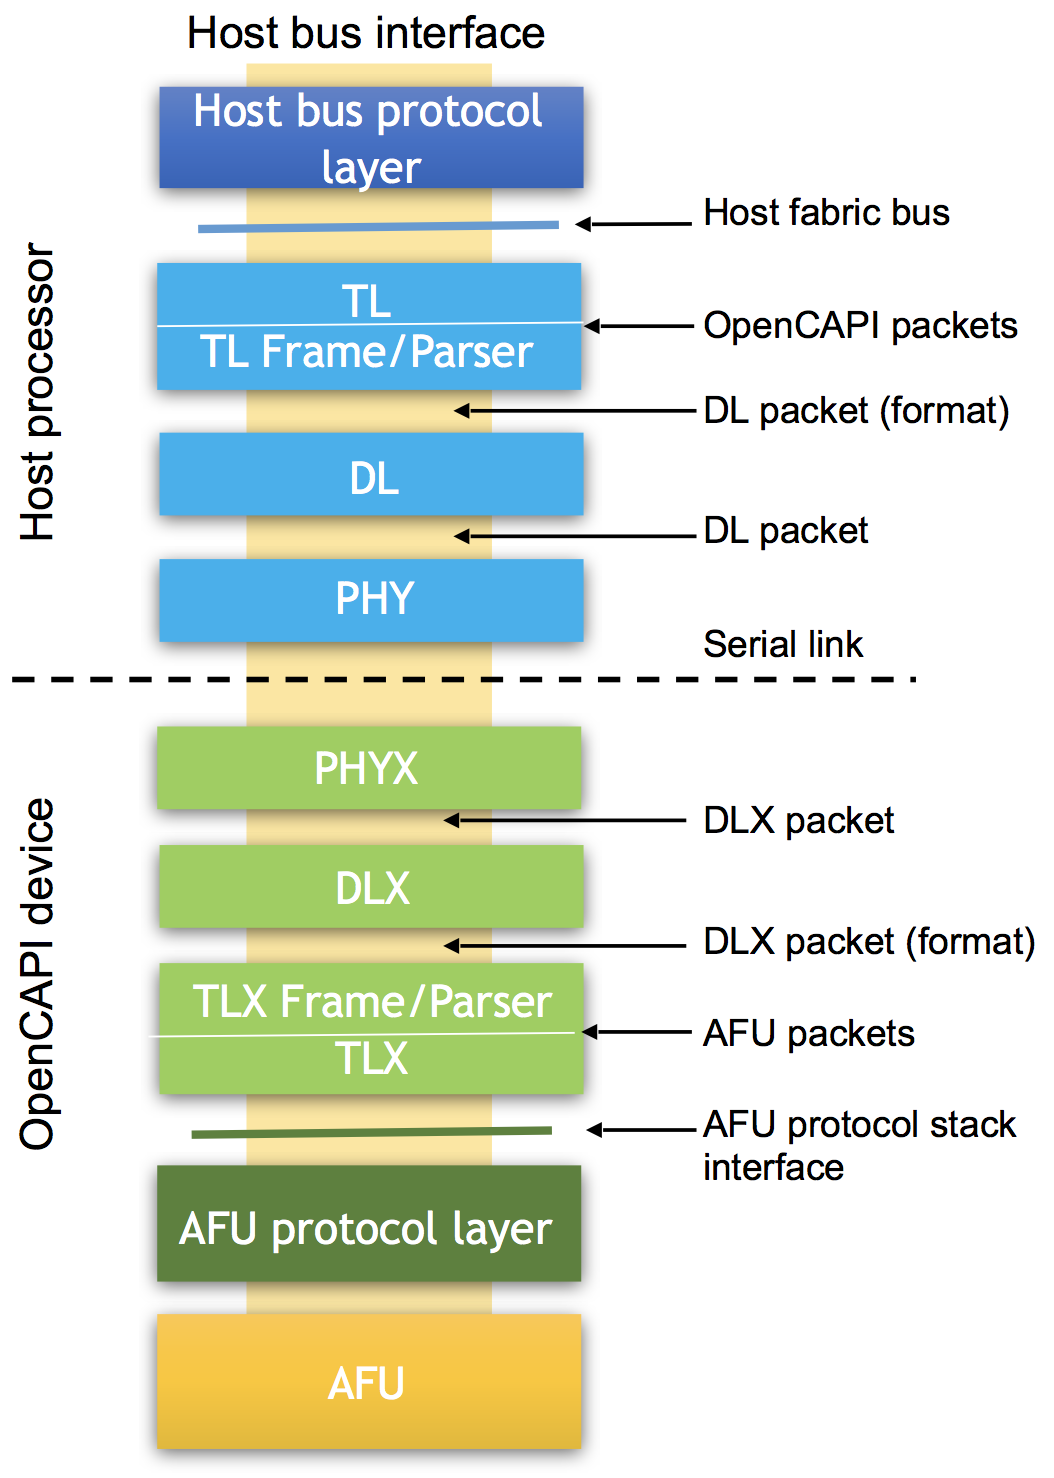
\includegraphics[width=0.55\textwidth]{2-ocapi-stack.png}
  \caption{The OpenCAPI stack from host to attached device \cite{opencapi-enablement}.}
  \label{fig:2-ocapi-stack}
\end{figure}



\subsection{Data Link Layer Frame Format}
\label{sec:frame}
Typically, packets are broken up in smaller pieces called flits, which stands for FLow control unIT. The first flit is the packet header and contains control information. Other flits, corresponding to the same packet, are data flits. In the context of OpenCAPI, the network packet is called a (DL) frame and the term packets is reserved for CAPP and AP commands and responses. The term TL packets acts as an umbrella for all different packets.\\
Both the TL and TLX framer and parser work with DL frames \cite{ocapi-dl}. A DL frame consists of one control flit and between zero and eight data flits, where at most four data flits belong to a single TL packet. Every flit is 64 bytes in size. Flits are transmitted starting at the lowest order control flit bytes and continuing in increasing address order. After that, the data flits are transmitted similarly. A control flit consists of an 8 byte DL content field and 56 bytes of TL packets, packed according to a predefined packing template. The OpenCAPI 3.1 TL specification \cite{ocapi-tl} adds a datum field to the control flit which embeds data smaller than 64 bytes within the control flit for improved frame utilization.

The DL content field contains both DL and TL generated subfields. Important are the DL injected CRC and TL injected TL template subfields. The CRC covers both the current control flit and the data flits from the previous control flit. Upon detection of an error, all data flits from the previous control flit are invalid and the transmitter is requested to replay the data flits. The final control flit never has any data flits, since it has to validate the last data flits using its CRC.\\
\autoref{fig:2-ocapi-frame} shows several DL frames and their respective control and data flits. The same colored flits indicate how a CRC in the DL content field corresponds to the data flit(s) from the previous control flit. The TL template subfield specifies the location of TL packets in the remainder of the control flit. The 56 bytes, or 448 bits, of TL packets in the control flit consist of sixteen, 28 bits, slots. TL packets differ in length and can consume between one and six slots per packet. Different package templates exist that indicate how many TL packets are present and how many slots they consume.

%DL: data run length, ACK count, CRC
%TL: bad data flit indication, TL template

\begin{figure}[h]
  \centering
  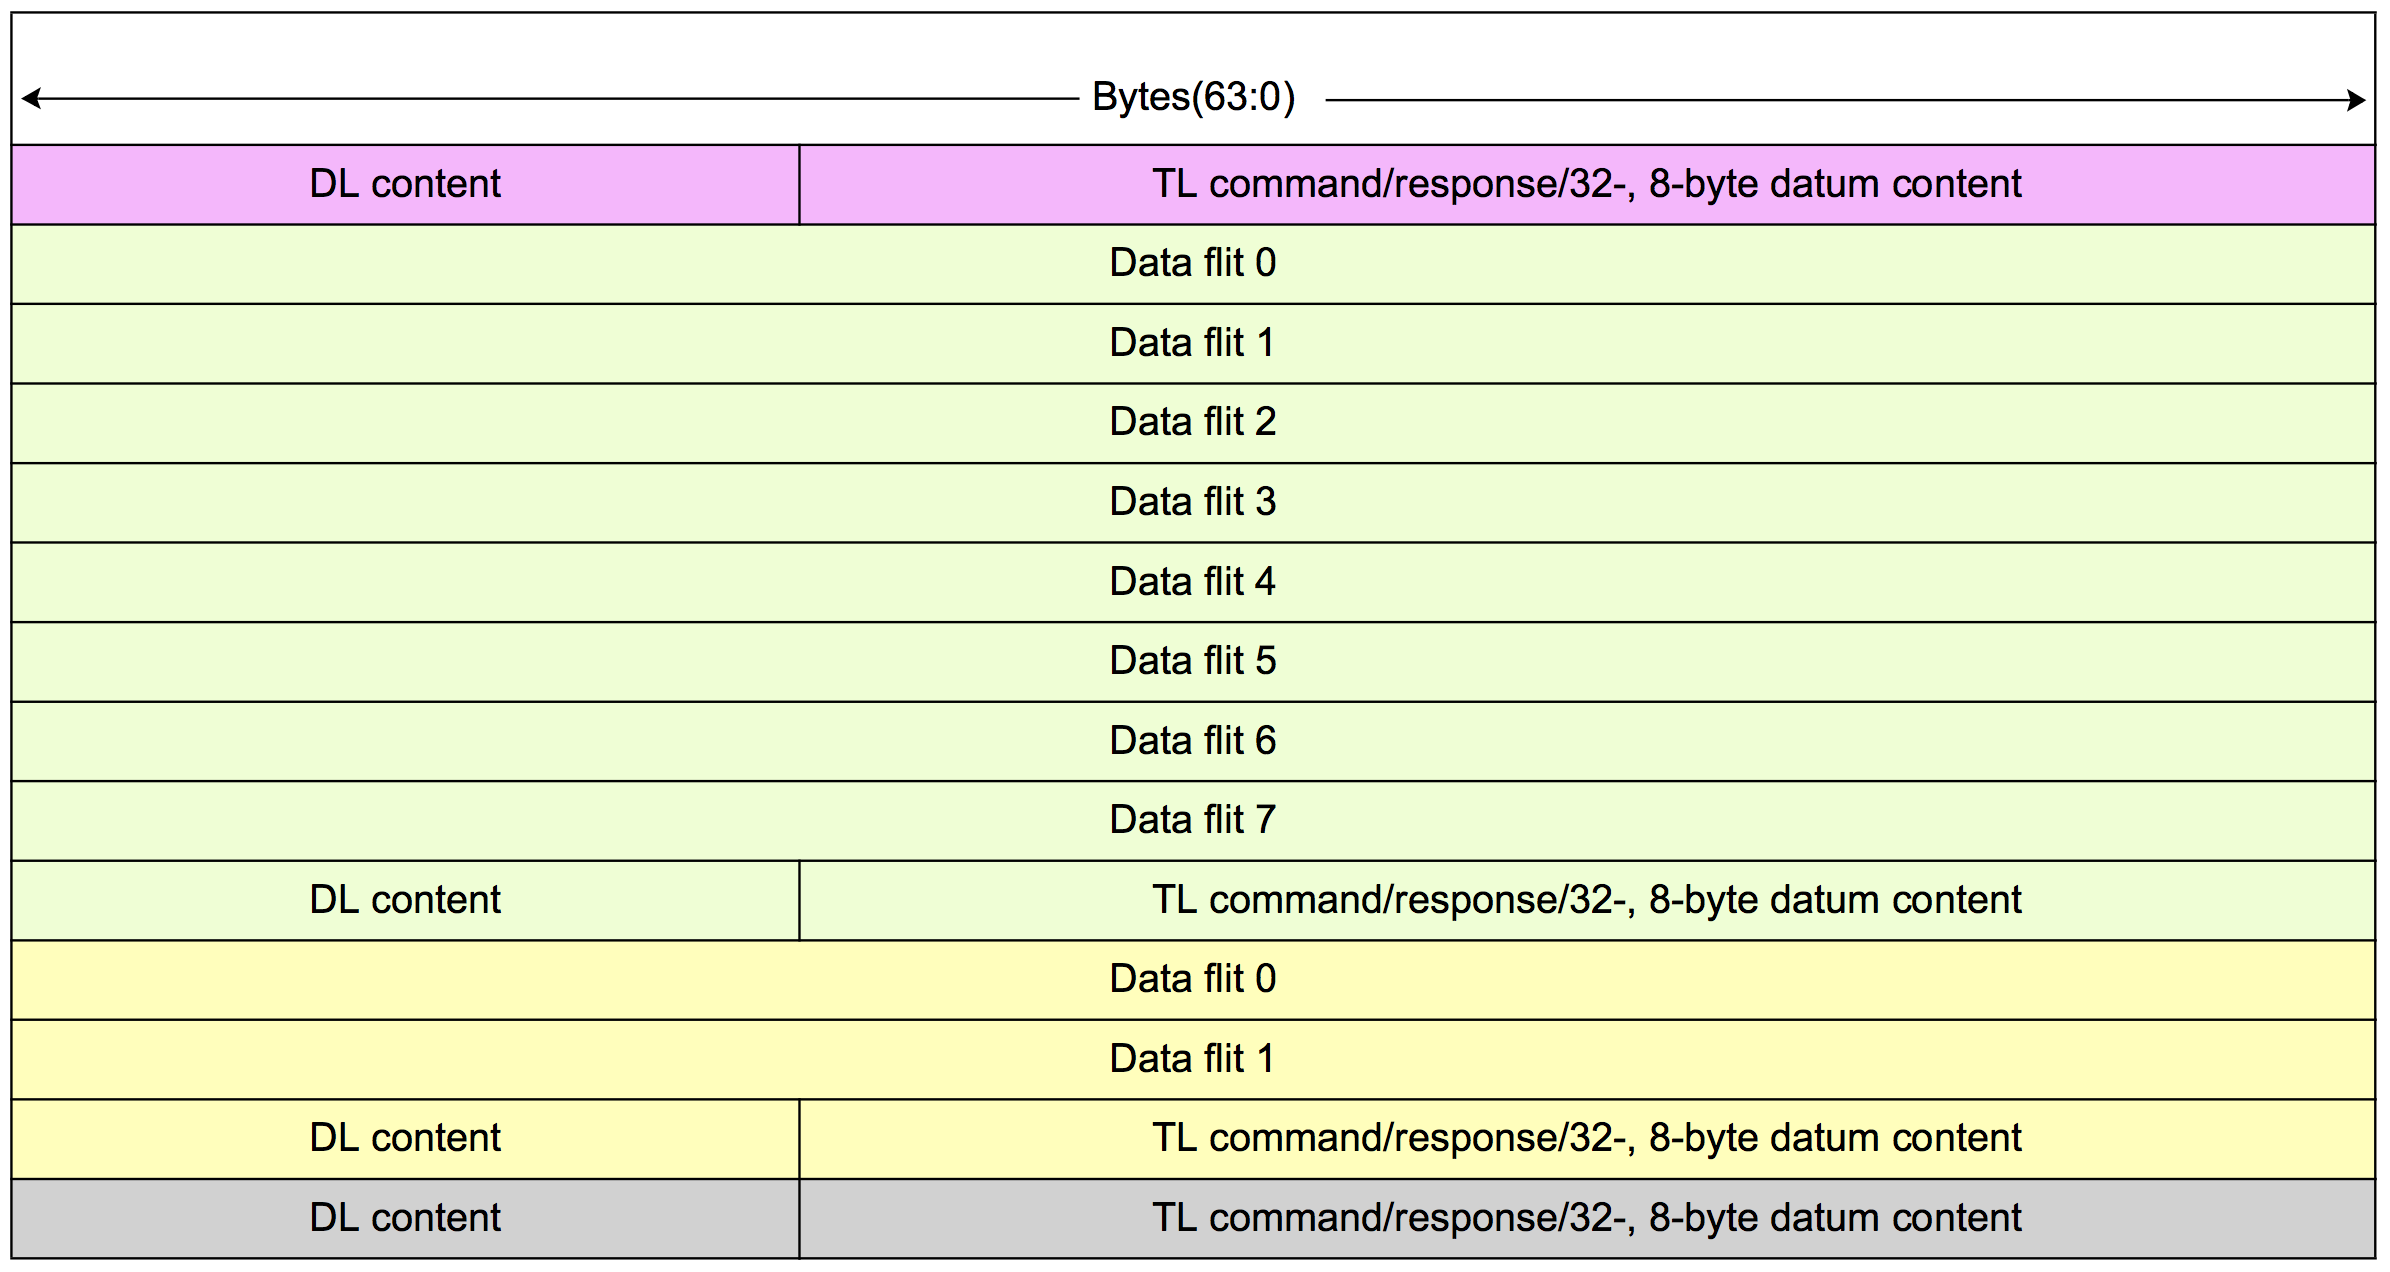
\includegraphics[width=0.85\textwidth]{2-ocapi-frame.png}
  \caption{Example of several DL frames showing the CRC control and data flit coverage \cite{ocapi-tl}.}
  \label{fig:2-ocapi-frame}
\end{figure}



\subsection{Transaction Layer Packets}
\label{sec:packets}
TL packets are control instructions that can be sent within a control flit \cite{ocapi-tl}. Depending on which side of the OpenCAPI link initiated the packet, the prefix CAPP (for the host) or AP (for the AFU) is used. There are several different types of packets, depending on the source. The host can issue from the following categories of commands. Bear in mind that each command requires a response (not listed below).
\begin{itemize}
  \item{\textbf{Address Translation} The host notifies the AFU that a previous address translation request has been completed.}
  \item{\textbf{Configuration Space} Reading and writing to the configuration space of the AFU is supported with specific commands.}
  \item{\textbf{Interrupt} The host updates the AFU regarding a previous interrupt request.}
  \item{\textbf{Memory Access} The host can read and write AFU memory at 64, 128 or 256 bytes data sizes at a time. It supports partial reads and partial and byte-enabled writes.}
  \item{\textbf{Metadata} An optional and implementation specific field to hold metadata for a data block held in memory.}
\end{itemize}
The AFU supports a different set of command categories.
\begin{itemize}
  \item{\textbf{Address Translation} The AFU can request address translation prefetching for an EA to warm up the address translation cache. This allows an accelerator to reduce translation latency when using a new page.}
  \item{\textbf{Assign acTag} The Address Context Tag (acTag) is used to index a host table containing the associated BDF and PASID. The BDF and PASID are used for address translation authorization and operation validation.}
  \item{\textbf{Atomic Operations} are supported to host memory (read, write, read-write). An accelerator can perform atomic operations in the same coherent domain just like any other host processor thread. Multiple variations are supported by hardware.}
  \item{\textbf{Interrupt} The AFU can request interrupt service on the host.}
  \item{\textbf{Memory Access} Currently, the AFU has no coherent cache. Therefore, read commands have a suffix to indicate no intent to cache. A coherent cache will be supported in OpenCAPI 4.0. A partial read is supported, as well as byte-enabled and partial writing.}
  \item{\textbf{Wake Host Thread} is an efficient low-latency mechanism used for communication between the host and attached device instead of either interrupts or host polling mechanism of host memory.}
\end{itemize}

Both the CAPP and AP side support a response packet for returning credits. As mentioned earlier, these are used for flow control.



\subsection{Coherent Accelerator Processor Proxy}
\label{sec:capp}

%\todo{- what are pages?\\
%}

The CAPP, in a host architecture agnostic context, contains all logic required on the host to enable OpenCAPI. \autoref{fig:2-ocapi-host-1} shows a possible system architecture where the CAPP is coherently connected to the rest of the host. An OpenCAPI device is then connected to the other side of the CAPP. Note that module names used here might change in the official documentation.\\
\autoref{fig:2-ocapi-host-2} shows CAPP implementations for the POWER9 \cite{curt}. It includes the OpenCAPI Processing Unit (OPU) and Nest Memory Management Unit (nMMU). The OPU consists of three stacks and each stack services two physical bricks of eight lanes. This brings the total to 48 lanes. Each stack consists of an XSL, and the DL and TL layers. The XSL handles address translation and has a dedicated ERAT/TLB of 64 entries and each entry represents a \SI{64}{\kilo\byte} page. Two stacks support OpenCAPI and are statically configured to use either OpenCAPI or NVLink 2.0 DL and TL layers, that in turn are connected to the PHY. The nMMU handles translation requests from other units than the CPU cores. It has its own ERAT/TLB with 8192 page entries, significantly more than the XSL.

%\begin{figure}[H]
%  \begin{subfigure}{0.5\textwidth}
%    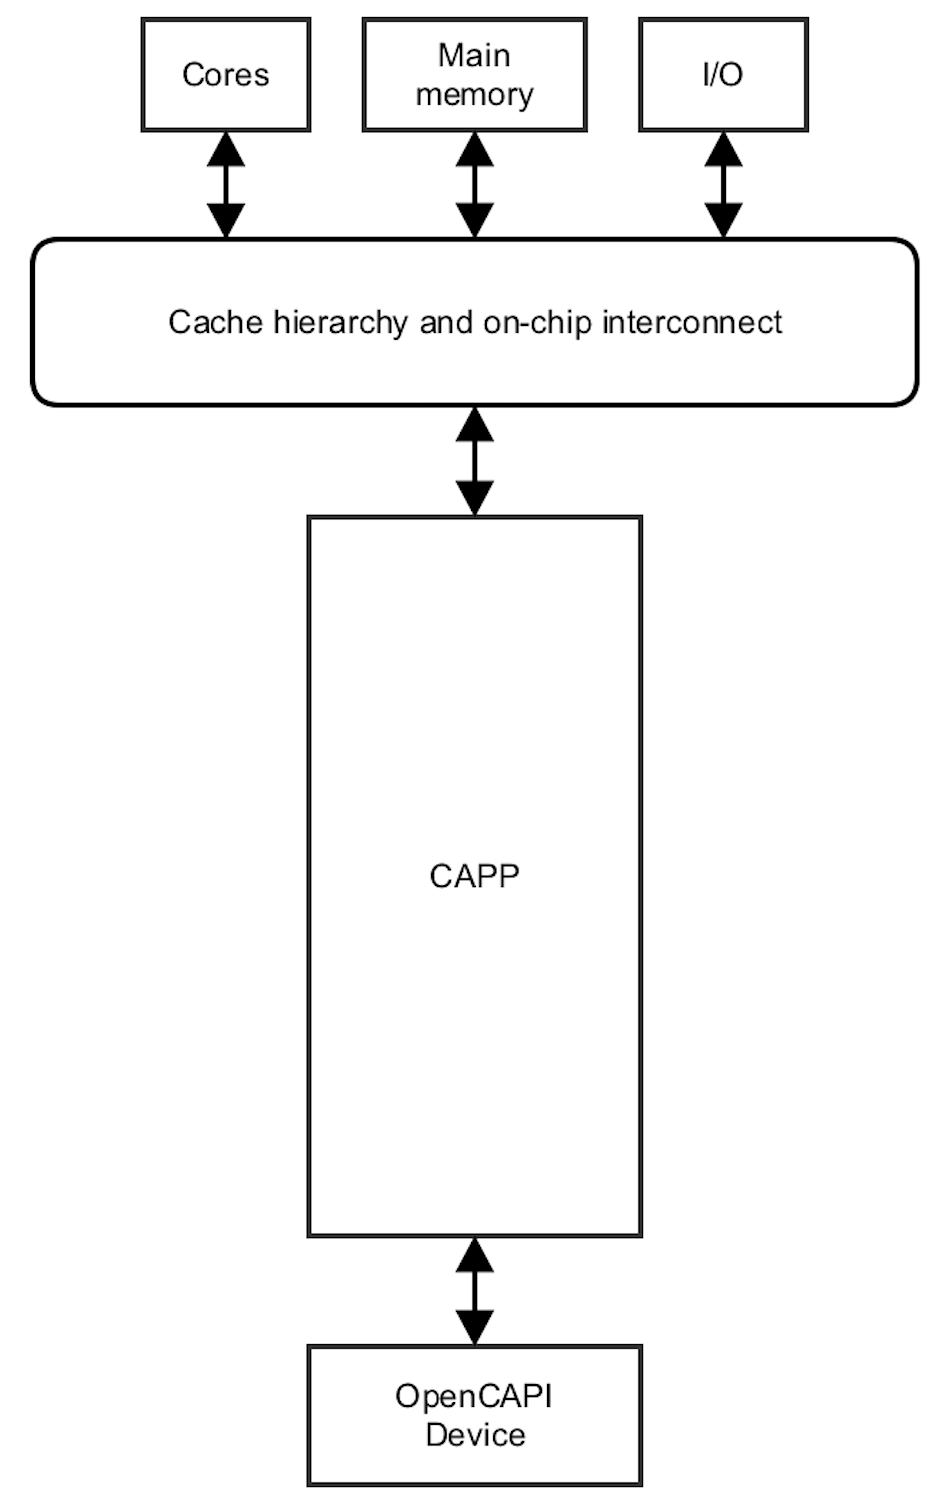
\includegraphics[width=0.6\linewidth]{2-ocapi-host-1.png}
%    \caption{Host architecture agnostic.}
%    \label{fig:2-ocapi-host-1}
%  \end{subfigure}
%  \begin{subfigure}{0.5\textwidth}
%    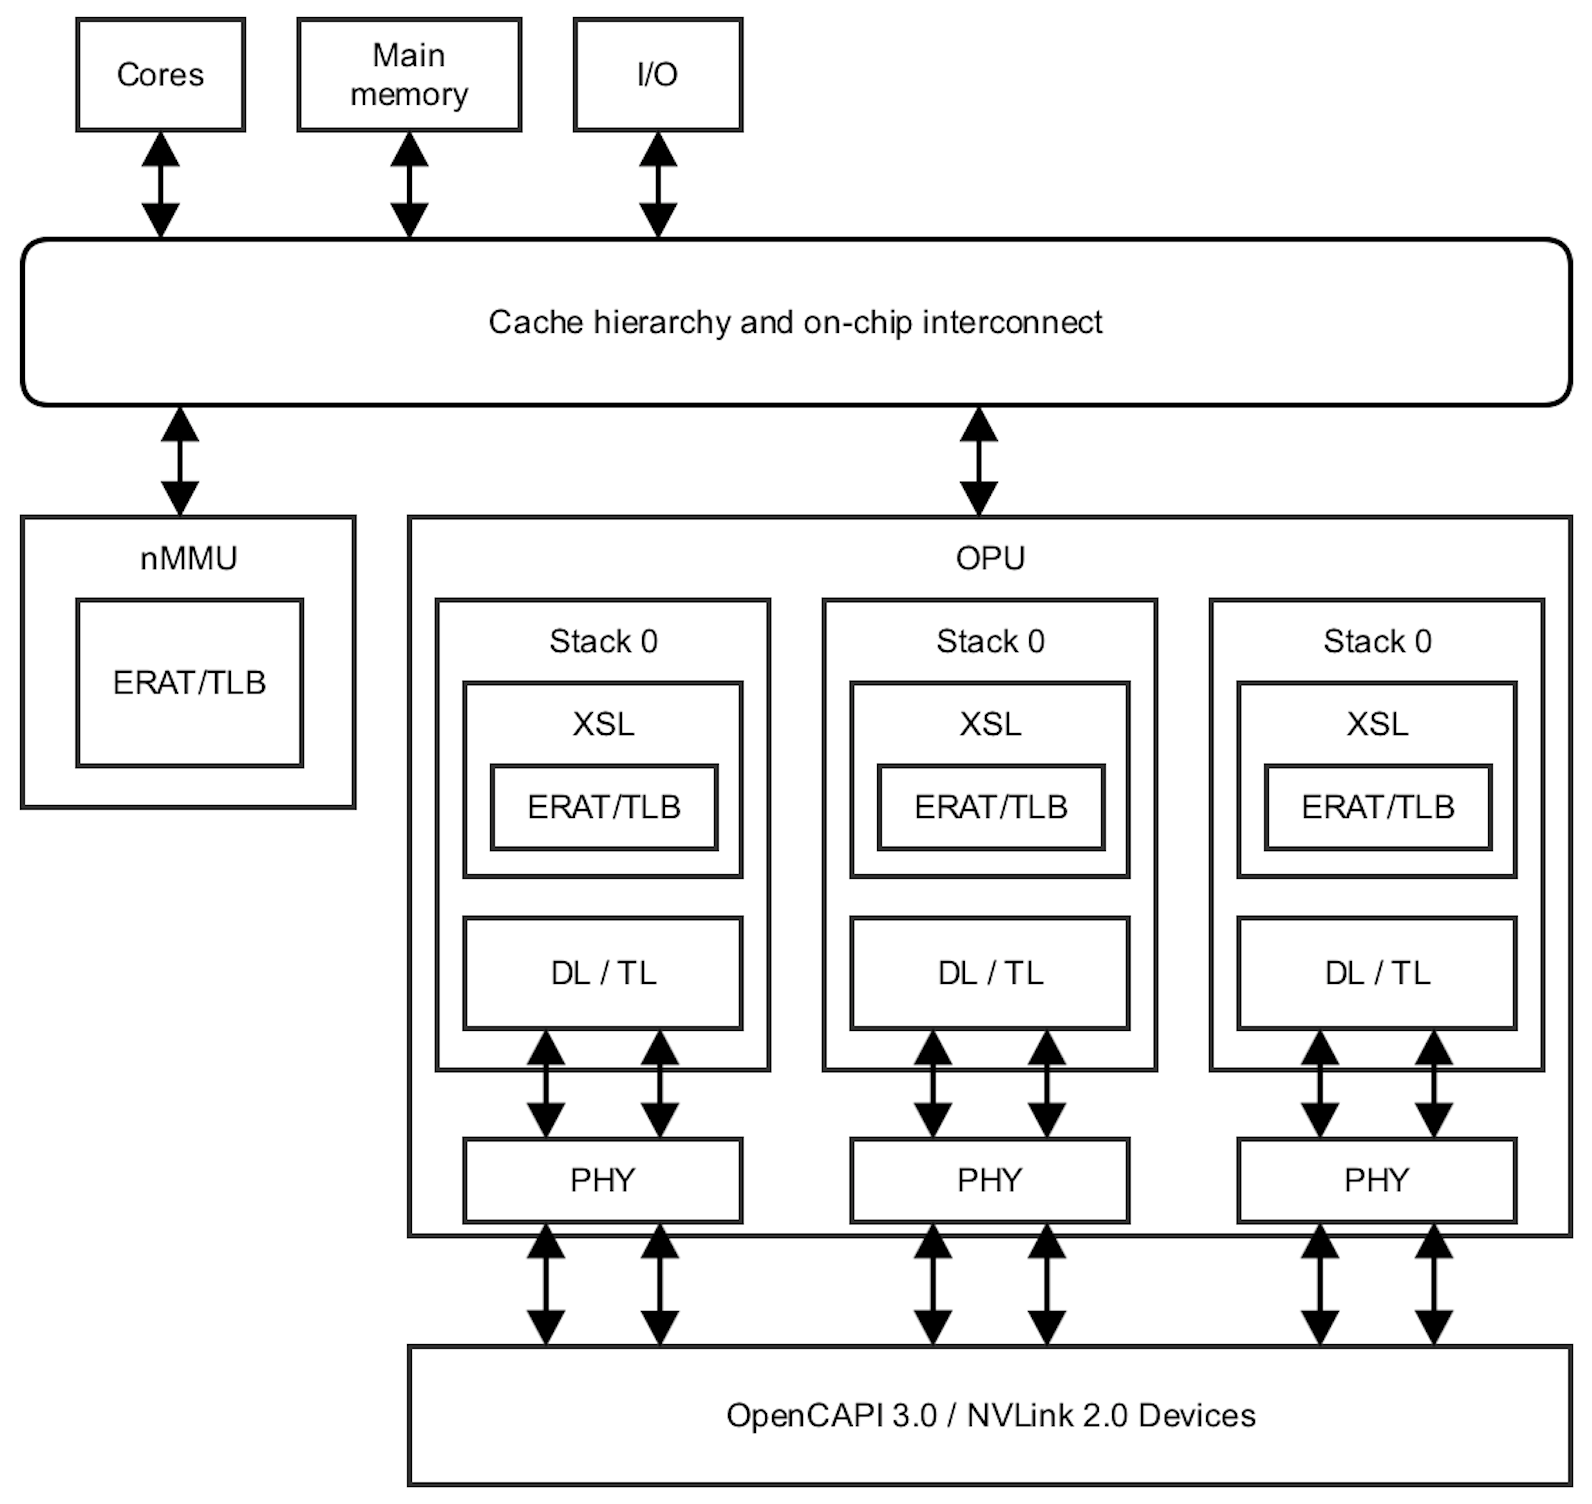
\includegraphics[width=1.0\linewidth]{2-ocapi-host-2.png}
%    \caption{POWER9 architecture specific.}
%    \label{fig:2-ocapi-host-2}
%  \end{subfigure}
%  \caption{System level view of OpenCAPI enablement on the host using the CAPP.}
%  \label{fig:2-ocapi-host}
%\end{figure}

\begin{figure}[htb!]
\ffigbox[\textwidth]
  {
    \begin{floatrow}
    \ffigbox[\linewidth]
      {\captionof{subfigure}{Host architecture agnostic.}
      \label{fig:2-ocapi-host-1}}
      {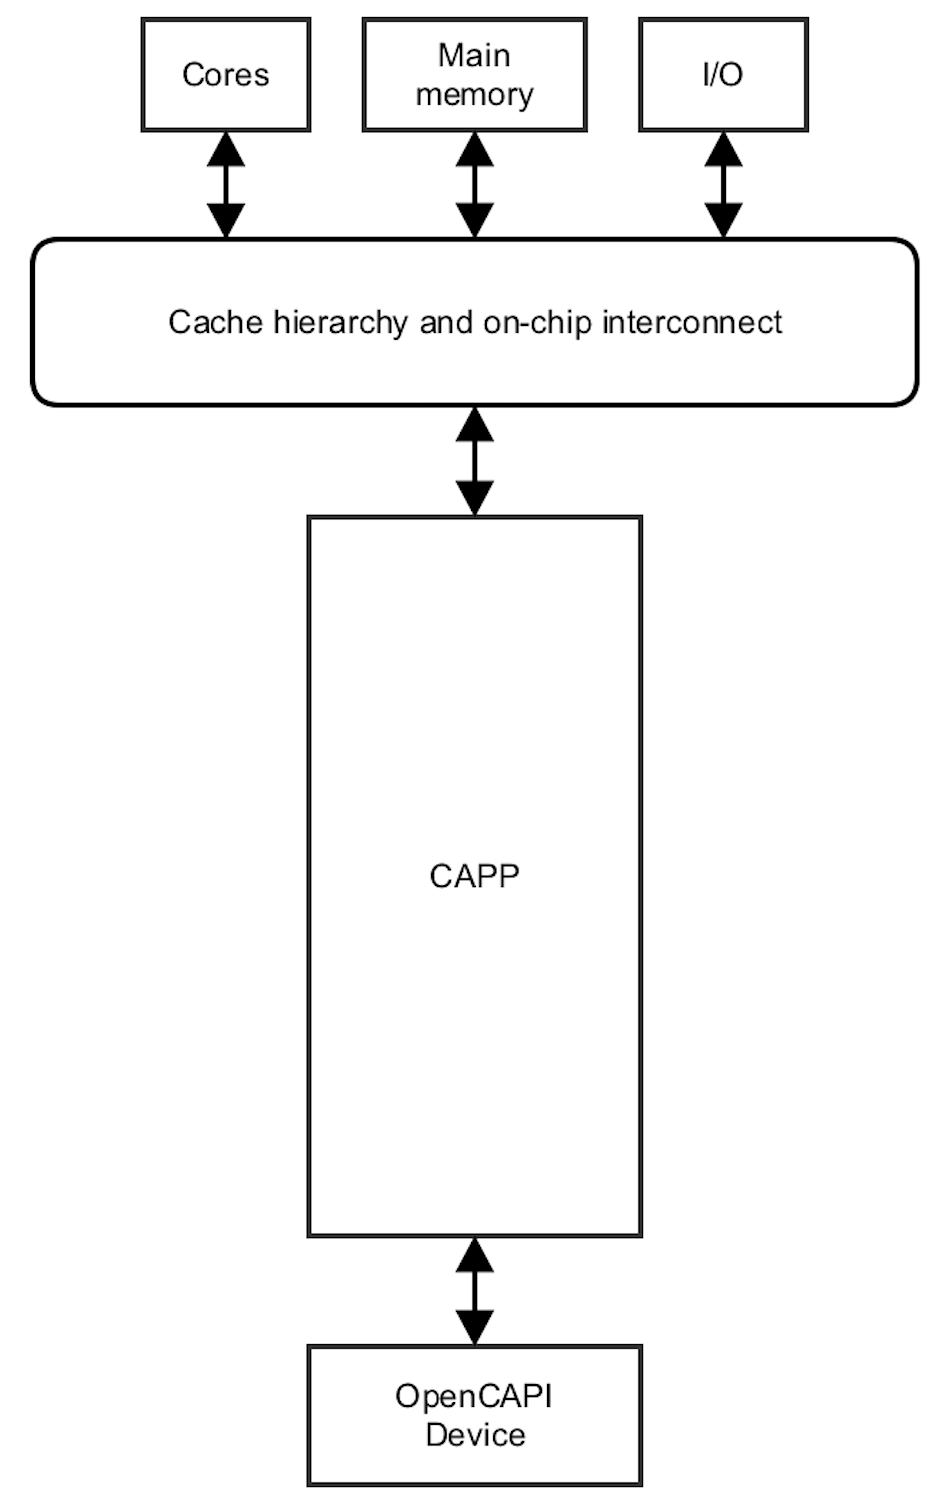
\includegraphics[width=0.50\linewidth]{2-ocapi-host-1.png}}
    \ffigbox[\linewidth]
      {\captionof{subfigure}{POWER9 architecture specific.}
      \label{fig:2-ocapi-host-2}}
      {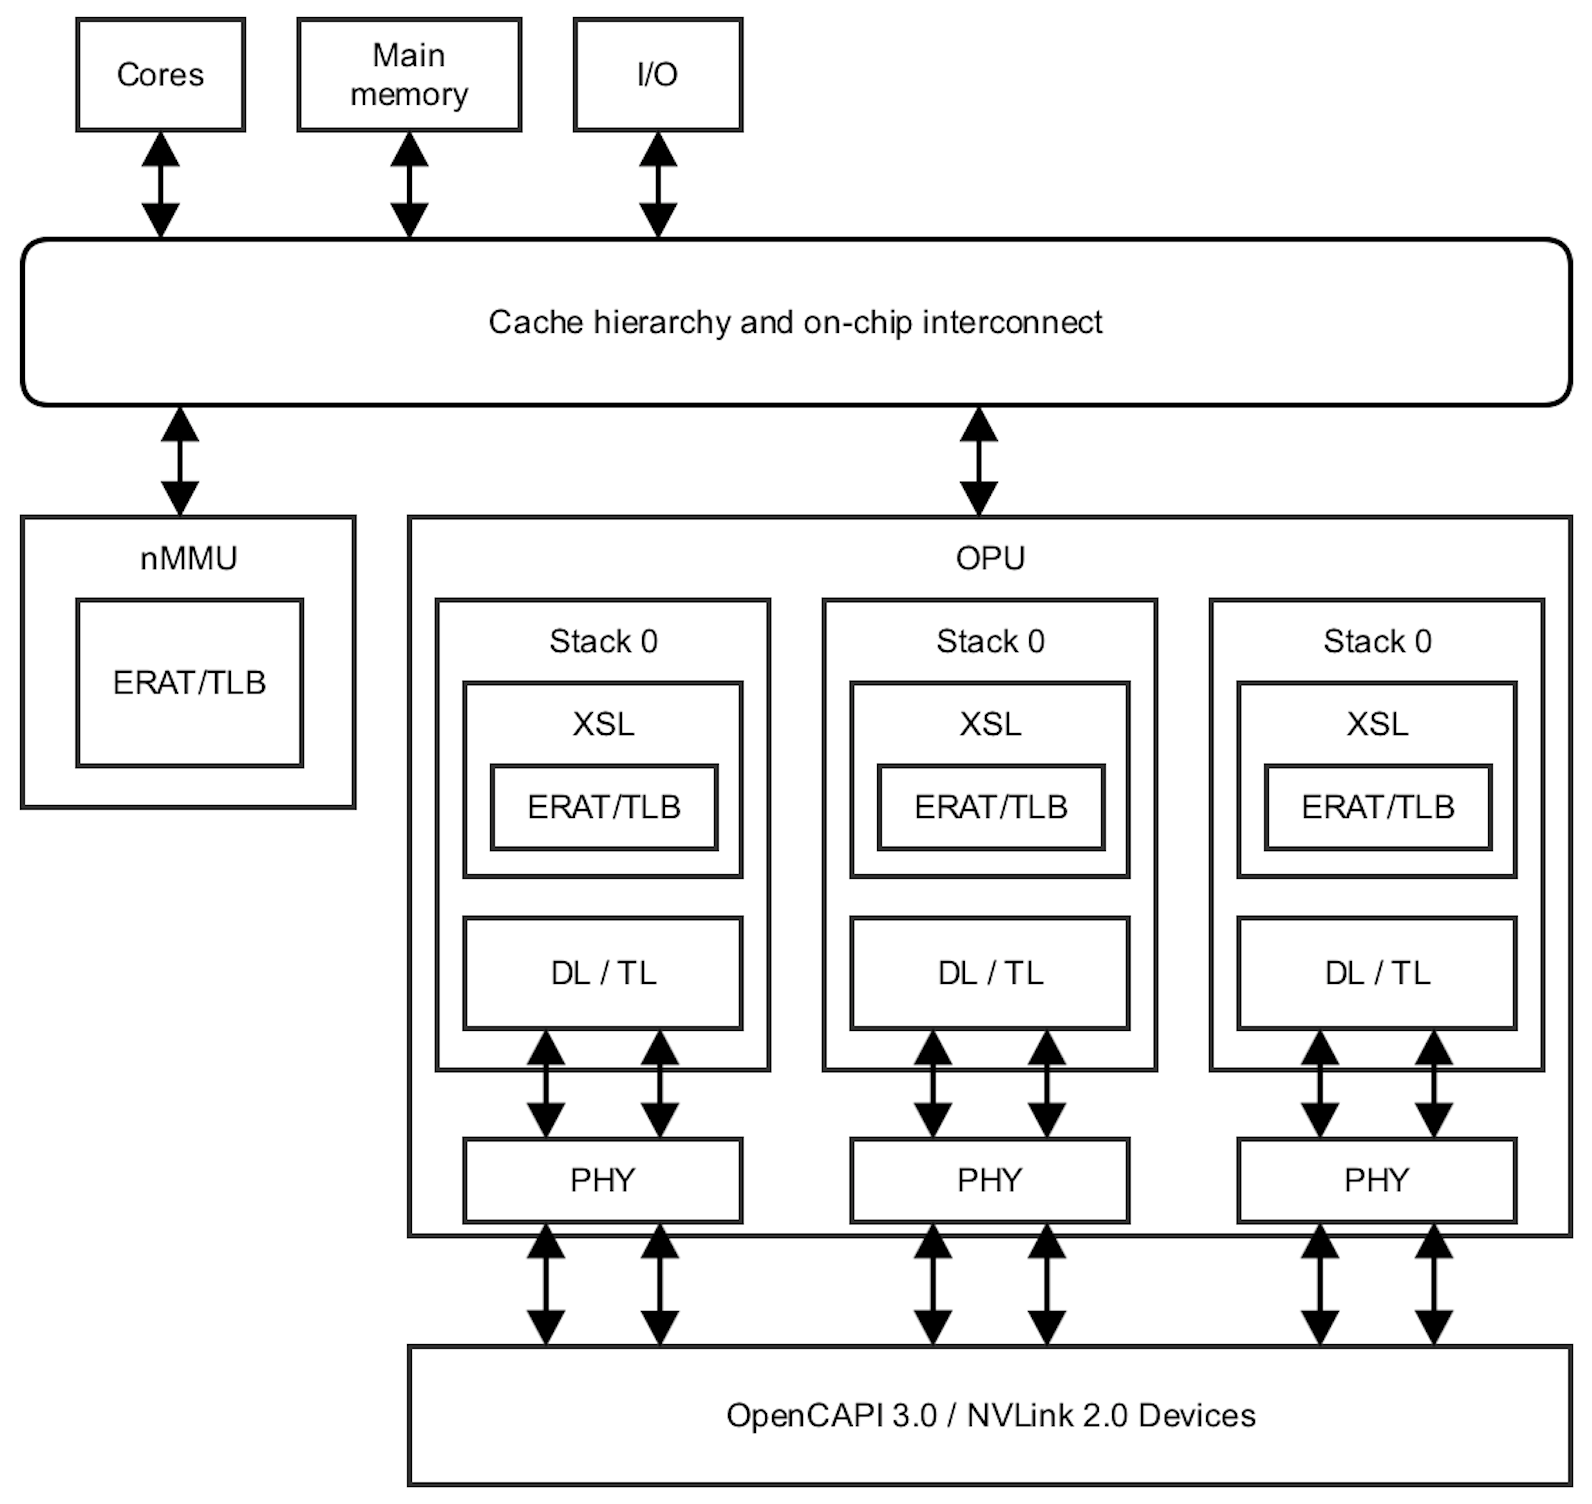
\includegraphics[width=0.85\linewidth]{2-ocapi-host-2.png}}
    \end{floatrow}%
  }
  {\caption{System level view of OpenCAPI enablement on the host using the CAPP.}\label{fig:2-ocapi-host}}
\end{figure}



\subsection{OpenCAPI Attached Device}
\label{sec:cacheline}
The CAPP is provided by the host architecture. On the FPGA side, the physical layer is supplied by the FPGA card vendor. Both the DLX and TLX are implemented using configurable resources on the FPGA and a reference design is provided by the OpenPOWER Foundation. The APL is an optional layer between the TLX and the AFU. Based on experience and customer feedback of CAPI 1.0 \cite{curt}, the OpenCAPI consortium decided to supply no specific interface between the TLX and APL in the sense that there is no cache or buffer present that the AFU can talk to directly. Instead, it provides an interface where TL packet opcodes can be sent to or received from the host.\\
\autoref{fig:2-ocapi-tlx} shows the presented TLX interface from a high level \cite{curt}. The TLX consists of a framer and parser, just like the TL. The parser receives frames from the DLX, unpacks the TL packets and splits the command and response packets, each presented at a separate interface. Each of these two interfaces consists of parsed control information from each TL packet and corresponding data payload. The data payload interface is 64 bytes wide, the same size as a data flit. If the payload of a single TL packet is more than one data flit, it takes multiple cycles to receive the entire data payload. The framer has similar interfaces, but packs TL packets instead to form control flits. There is also a configuration module present on the AFU which holds registers for configuration of the TLX. For example, to enable certain packing templates. There are separate interfaces for this module, not shown in the figure. The TLX also manages credits and each interface has a credit interface in opposite direction. The TLX parser also gives credits back to the TLX framer.\\
The latest generation of Xilinx FPGAs are used that allow an increased operating frequency of up to \SI{450}{\mega\hertz}. To minimize latency, the target frequency of the DLX and TLX is \SI{400}{\mega\hertz}. Each of the four data interfaces can supply up to 64 bytes per cycle at the target frequency. Typically, highly pipelined FPGA designs can reach up to \SI{250}{\mega\hertz}. If an AFU operates at \SI{200}{\mega\hertz}, it will seem like OpenCAPI provides 128 bytes per cycle. This is also the size of a cache line in the POWER architecture.

\begin{figure}[H]
  \centering
  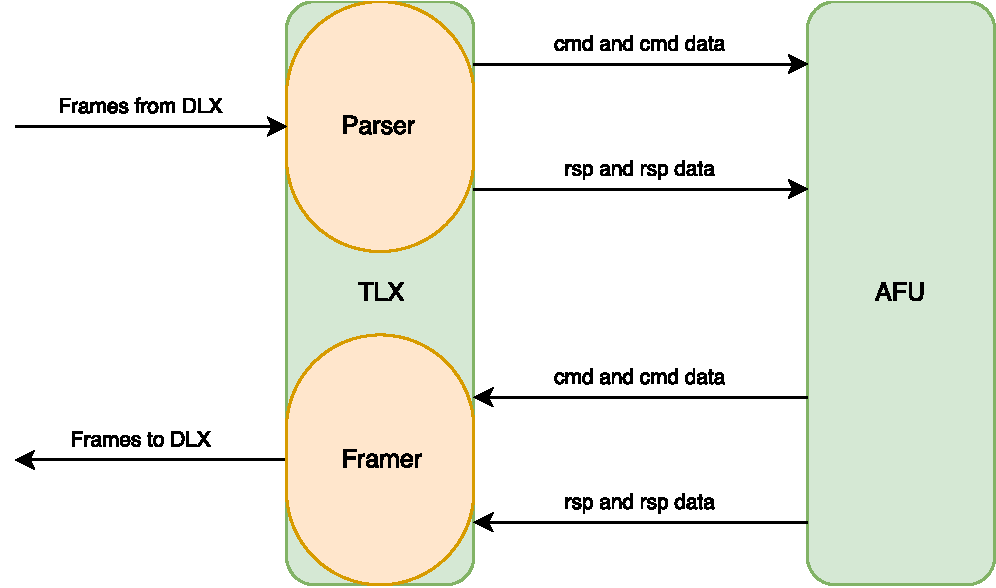
\includegraphics[width=0.55\textwidth]{2-ocapi-tlx.pdf}
  \caption{Interface between the TLX and APL or AFU, depending on the AFU design.}
  \label{fig:2-ocapi-tlx}
\end{figure}

An OpenCAPI device may have three physical address spaces. The configuration space is in a separate space from the MMIO and system memory spaces. These spaces share a PA space and the host can differentiate between the two since the system memory space always starts at offset zero of the PA, while the MMIO space starts at a fixed configured offset from zero. The MMIO offset is configured using a BAR (Base Address Register) and multiple BARs are present to service multiple attached devices.
\begin{itemize}
  \item{\textbf{Configuration space} may be used for configuring the TLX or AFU. It is accessed by using the dedicated read and write commands. A reference configuration space module will be provided by the OpenCAPI consortium.}
  \item{\textbf{MMIO space} may be used for configuration of the AFU and is mapped in the system memory address space.}
  \item{\textbf{System memory space} is a memory space owned by the OpenCAPI device and is mapped to the system's RA space. This memory is coherently accessed using the load/store model used by the host.}
\end{itemize}

A typical usage model is to write a work pointer in an AFU MMIO register or by communication through shared memory. The MMIO module is flexible in the sense that the MMIO base address register and sizes can be configured by the AFU designer. Also configuration registers are present on a per-process basis. The MMIO module is provided by the OpenCAPI consortium and can be integrated directly within a design.

%The following is from section 1.5 in the TL 3.1 tion.

%The configuration space is accessed by using the dedicated read and write commands. The PA specified for this space is separate from the system memory space and the MMIO space. The host may:
%- Provide a configuration address BAR to access this space using a direct access load/store model.
%- Provide an MMIO register set to access this space using an indirect access method.

%The MMIO space shares the PA space used by the system memory space. It is specified by a fixed offset from PA 0 specified in the OpenCAPI device’s configuration space. The host differentiates the MMIO spaces of different OpenCAPI devices by providing a configuration address BAR for each attached device.

%The system memory space is memory space owned by the OpenCAPI device that is mapped to the host’s system memory. The PA for system memory space is defined to start at offset 0. The host differentiates between the different system memory spaces of different OpenCAPI devices by providing a configuration address BAR for each attached device.

%Real addresses (RA) are mapped into the physical address (PA) space specified for a device. This eliminates any requirement placed on the OpenCAPI device to have knowledge of the host’s real address space or how the OpenCAPI device’s PA space is mapped into it. The following rules place restrictions on the OpenCAPI device’s specification of its PA space.



\subsection{Address Spaces and Translation}

%\todo{- Why are there three levels of address translation? RA, EA and PA. Spec talks about function 'convert2PA'. Does the CAPP/OPU have RA2PA translation?\\
%- Curt: are there opcodes for warming up the TLB? I think Andy once mentioned that it is stupid that the TLB(s) are not warmed up during system start-up. TL spec: warming up = The process of loading or populating a cache with a set of valid data.\\
%- Curt: POWER uses three types of addresses. EA, RA and PA. Where does the translation from one to another happen (specifically, where in the drawing)?
%The AFU only uses an EA.  The nMMU translates an EA to an RA internally.  The PA is the physical address in memory (mapped to specific location in a DIMM by the memory controller).\\
%- A program on the P9 or the AFU only see an Effective Address EA for addressing the system address map for OCAPI 3.0 when it masters commands.  If the program wanted the AFU to fetch memory from a DIMM is would give it an EA.  The AFU sends the EA across the link.  The XSL translates the EA to a Real Address (RA).  To do this first it looks in its ERAT.  If it misses the XSL ERAT it forwards the request to the nMMU.  The nMMU will look in its ERAT before walking the page table to resolve the translation into a RA.  The RA is what the fabric bus uses to communicate with caches and DIMM memory.  Physical Address (PA) would be what the memory controller resolves to a physical DIMM address.  An MMU translates an EA to RA via page/segment table walking.  The nMMU handles it for nest units, and the cores have their own MMU as well.  The ERAT is just a TLB that is searched before invoking a page table walk.\\
%- I meant it only uses an EA for mastering commands to memory.  The PA you mention is for slave commands.  That is a PA within the AFU address space (either config or MMIO).  It represents a physical address within the AFU (most likely register).  Some other program accessed this with an EA that was translated to an RA.  The RA matched a range within the NPU that configured it as AFU memory.\\
%- The entire system address map is based on Real Addresses.  That entire map consists of physical DIMM memory (main system memory), PCIe memory, GPU memory, etc.  Each of the regions has a base/size region of the RA that maps to it.  You can think of the physical address as the RA minus the base so it maps directly to a location within the memory device.\\
%}

While address translation is present on the host and managed by hardware, it is of interest to the AFU designer since it can greatly influence performance regarding translation misses. Page table walks are very expensive and take many cycles to complete \cite{curt}. Therefore tuning the AFU to optimally use the TLB and warming up the TLB is a good practice.



\subsubsection{Address Spaces in the POWER Architecture}
\label{sec:spaces}

%\todo{- Curt: Have some figure to show how EA, RA and PA are converted/translated into each other.}

Three different address spaces exist in the OpenCAPI and POWER architecture.
\begin{itemize}
  \item{\textbf{Effective Address (EA)} is the address seen by a program, also known as a virtual address.}
  \item{\textbf{Real Address (RA)} is the address used to access the entire system address map. The entire map consists of physical DIMM memory, PCIe memory, GPU memory, etc. Each of the regions has a base and size region of the RA that maps to it. These addresses are for example used within the fabric on the POWER9 to communicate between caches and DIMM memory.}
  \item{\textbf{Physical Address (PA)} is the address used by a physical memory source, such as a DIMM or local memory of an attached device. You can think of the physical address as the RA minus the base. It maps directly to a location within the memory device.}
\end{itemize}

%From TL spec 3.1:
%EA = Effective address. This is the address as seen by a program. Some host architectures refer to this as a virtual address (VA). Mapping from an EA to an RA requires address translation services.
%RA = Real address. A real address is the result of address translation of an EA. Some host architectures refer to this as a physical address.
%PA = Physical address. This refers to the address space owned by an AFUM device. The host converts the RA to the AFUM device’s physical address space using configuration settings in the host that are deter- mined during initialization of the attached OpenCAPI device.
%A PA is not the result of address translation of an EA as might be the case in some host architectures. The host maps the device’s PA into its own (RA) address space.

The system memory address space includes all addresses within the system and uses real addresses. Main memory is the portion that is normally backed by physical DIMMs and marked coherent. This can be cached by processor caches and coherency maintained. MMIO (memory mapped I/O) is mapped into the system memory map, but it is marked in the page tables as non-cacheable. This includes the PCI Express devices MMIO regions, AFU MMIO regions, as well as the processor MMIO addresses. MMIO regions consist usually of registers and are used for configuration of the system and communication with the device driver for I/O devices. It is a region in the system memory map because it is accessed across the fabric from a program running inside a core to communicate with the attached device via EA-RA translation.



\subsubsection{Address Translation}
Taking a look at \autoref{fig:2-p9-system} again, the fabric uses real addresses. If a memory location within a DIMM is accessed, the memory controller resolves a physical address from the real address. Cores have their own MMU in order to translate an effective address to a real address via page/segment table walking. An effective address will be translated to a real address if a memory location has to be accessed outside of the current core.\\
In OpenCAPI, all translations happen on the host and occur either in the OPU or nMMU. In CAPI 1.0, part of the translation was located on the FPGA (in the PSL). Moving the address translation to the host reduces design complexity of attached devices. Since an attached device never has access to a physical address, malicious attached devices are not able to access unauthorized memory locations, such as addresses belonging to kernel or other applications.\\
The AFU only uses effective addresses for mastering commands to host memory, that are translated on the host to real addresses. When the AFU acts as a slave and receives commands from the host, physical addresses are used to access the three different physical address spaces mentioned in Section \ref{sec:spaces}. These physical addresses have been translated from program EA, to system RA, to PA. The host converts the RA to a PA using configuration settings in the host that are determined during initialization of the attached OpenCAPI device.\\
Real addresses are mapped into the physical address space specified for an OpenCAPI device. This eliminates any requirement placed on the OpenCAPI device to have knowledge of the host’s real address space or how the OpenCAPI device’s PA space is mapped into it. The PA for CAPP commands is all translated in the host (MMIO, Config, host memory). The host has programmable base address (BAR) and offset registers for everything. The PA space in the FPGA is either config space (indicated by command type), MMIO (indicated by matching the AFU's base address), or host memory (if it doesn't match the AFU's BAR).

% Mastering commands means AFU is 'master' of the interconnect. So when it sends out TL command packets.
% When the AFU acts as a slave, it services host commands.



\subsubsection{Address Translation Example}
As an example, consider a POWER9 with an OpenCAPI-attached device. A program on the processor only sees an Effective Address for addressing the system address map. If the program requests the AFU to fetch data from host memory it uses an EA. The AFU sends the EA across the OpenCAPI link and the XSL translates the EA to a Real Address (RA). To do this, first it looks in its ERAT. If it misses the XSL ERAT it forwards the request to the nMMU. The nMMU will look in its ERAT before walking the page table in host memory to resolve the translation into an RA. If the page walk fails it will return a bad status to the OPU, and it will generate a fault interrupt to resolve the fault.\\
In the other direction, a program uses an EA and the OS sets up mappings between a page to a physical resource. To communicate across the fabric, the program EA is translated to an RA. The RA is then matched to a range within the OPU that is configured as AFU memory and translated from RA to PA.



\section{Coherent Programming Model}
%\todo{
%- No cache coherence: a solution would be to implement coherency is software, but that introduces a lot of overhead. to cover the latency a solution has to be found. a local mem on the fpga is needed. how to move data to it? following stuff in requirements: accelerators like database operators can operate under the offload paradigm.\\
%}

OpenCAPI enables new, easier and more natural programming models, as found on multi-core systems, for IO that was not possible with the traditional approach. Attached devices are more easily accessible due to the shared virtual memory space and appear as peers to the processor cores. Also the setup and completion phases, by interacting with device drivers, have been simplified and made faster. Combining this with attaching devices with a low-latency interconnect, the attached devices become tightly coupled that allows for thread-level parallelism between the application running on the host and the attached device.



\subsection{Coherent Shared Virtual Memory}
The approach of OpenCAPI (and CAPI for that matter) offers a virtual address space shared between the processor caches and the attached device \cite{opencapi-jeff-preso}. The host and accelerator can coherently access each others physical memories. This removes the problem of having multiple copies of the same data in a traditional IO model (see Section \ref{sec:copies}) and reduces setup and completion time significantly for an application wanting to use the attached device. Typically, this might take \SI{12.8}{\micro\second} as shown in \autoref{fig:2-flow-model}. Now it might take as little as \SI{0.36}{\micro\second}.\\
Not only can the host use atomic operations, but also the attached device has a vast set of atomic operations to implement synchronization operations. A special wake host thread opcode can be used for communication as well.\\
%OpenCAPI is also flexible in configuration. If the attached device does not want to support atomics for example, you tell the host and atomics will be send out as special read and write operations.\\
The shared virtual memory space also allows programmers to dereference pointers everywhere, while previously host pointers could only be dereferenced on the host and vice versa \cite{benton}. This removes the manual movement of data between the host and attache device. Overall it simplifies the programming model since the attached device operates as a peer to the other processor cores. With the traditional IO model, sharing an attached device between applications was difficult because pinned memory belongs to only one application and cannot be shared. If the attached device supports multiple hardware buffers, multiple applications could use the device. The number of applications is dependent on the hardware. OpenCAPI allows for sharing the accelerator between applications due to a special feature in the standard (context bits).\\
With CAPI, a coherent cache was present on the accelerated device. This allows for even more programmer flexibility and lower latency for highly referenced data. However, this feature is absent in OpenCAPI 3.0 but will return in OpenCAPI 4.0.

%\todo{- Make own figures (two subfigures).}

\begin{figure}[H]
  \centering
  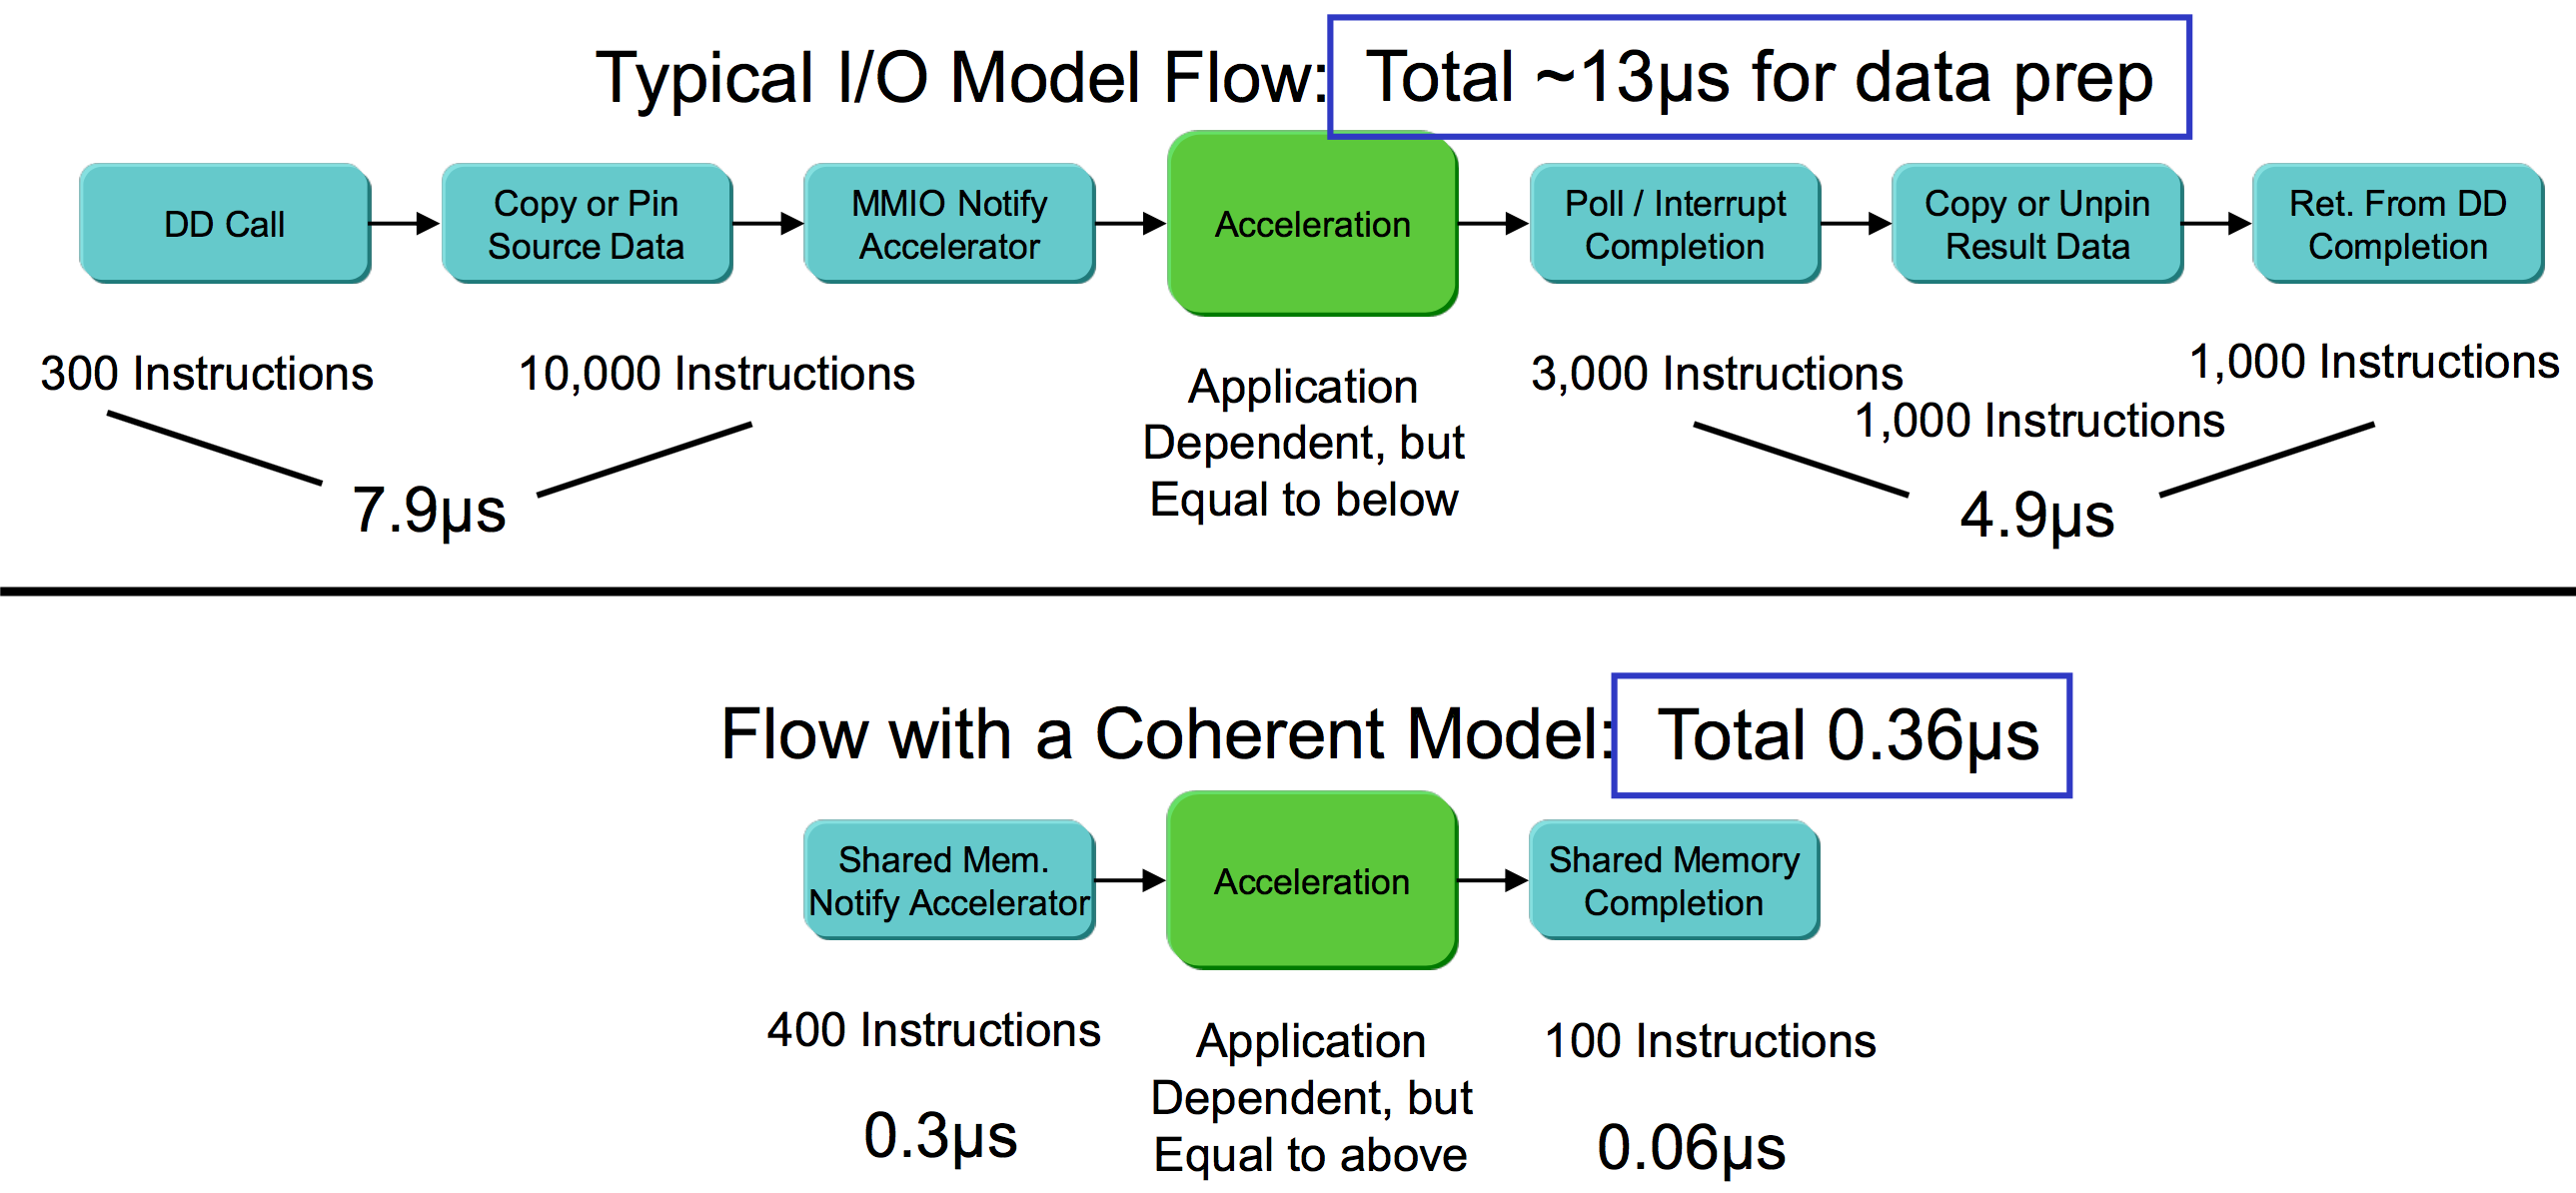
\includegraphics[width=0.80\textwidth]{2-flow-model.png}
  \caption{Traditional IO device setup and completion flow versus the OpenCAPI flow \cite{opencapi-enablement}.}
  \label{fig:2-flow-model}
\end{figure}



\subsection{Accelerator Paradigms}
Traditionally, an offload paradigm was used for accelerators, shown in \autoref{fig:2-ocapi-paradigm-1}. \autoref{fig:2-ocapi-paradigm} shows current and new paradigms enabled by OpenCAPI. A perfect example is an application that uses pointer chasing or linked lists \cite{opencapi-forum}. This was not possible because pointers were not able to be dereferenced since the processor and IO device did not share the same address space. Other applications could include using both the shared host memory and local memory of the accelerator, since accessing host memory has a very low latency. An example of such a bi-directional accelerator is shown in \autoref{fig:2-ocapi-paradigm-5}.

\begin{itemize}
  \item{\textbf{Memory transform} is the traditional offload paradigm. GPUs fall into this category.}
  \item{\textbf{Needle-in-a-haystack engine} processes a large data set from disk for example and filters specific data of interest.}
  \item{\textbf{Egress transform} processes outgoing data, as it leaves the system. Examples are compression and encryption on its way to centralized storage.}
  \item{\textbf{Ingress transform} processes incoming data, for example from a NIC, and places the output in host memory. An example could be decompression and decryption.}
  \item{\textbf{Bi-directional transform} can be used for a hash-join database operator using a database located on disk. The hash table can be build in host processor memory. Stream through data from disk and do computations that while fetching hash table from host memory.}
\end{itemize}

\begin{figure}[H]
  \begin{subfigure}{.5\textwidth}
    \centering
    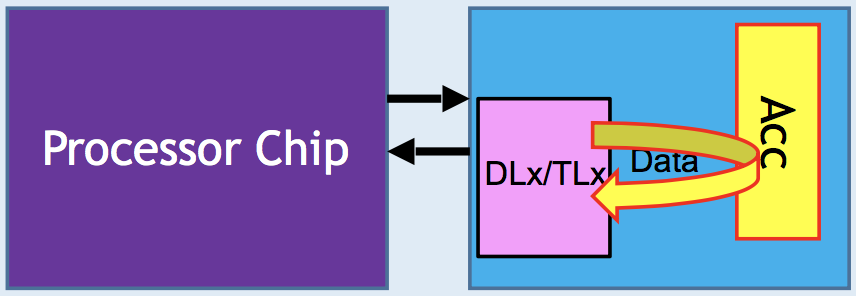
\includegraphics[width=0.90\linewidth]{2-ocapi-paradigm-1}
    \caption{Memory transform.}
    \label{fig:2-ocapi-paradigm-1}
  \end{subfigure}%
  \begin{subfigure}{.5\textwidth}
    \centering
    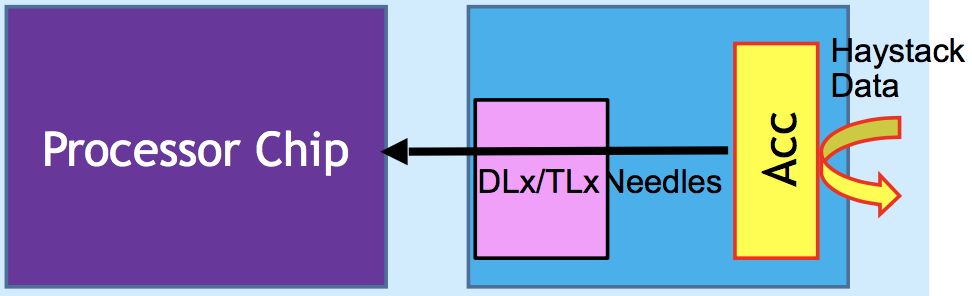
\includegraphics[width=0.95\linewidth]{2-ocapi-paradigm-4}
    \caption{Needle-in-a-haystack engine.}
    \label{fig:2-ocapi-paradigm-4}
  \end{subfigure}\\[1ex]
  \begin{subfigure}{.5\textwidth}
    \centering
    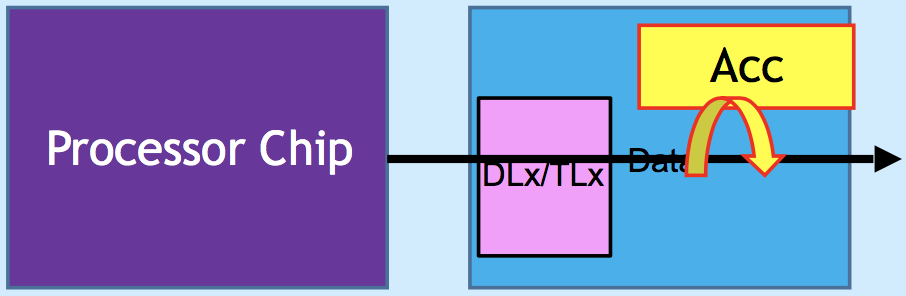
\includegraphics[width=0.90\linewidth]{2-ocapi-paradigm-2}
    \caption{Egress transform.}
    \label{fig:2-ocapi-paradigm-2}
  \end{subfigure}%
  \begin{subfigure}{.5\textwidth}
    \centering
    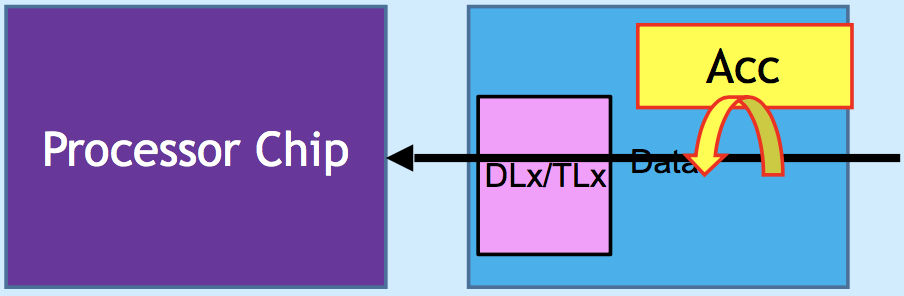
\includegraphics[width=0.95\linewidth]{2-ocapi-paradigm-3}
    \caption{Ingress transform.}
    \label{fig:2-ocapi-paradigm-3}
  \end{subfigure}\\[1ex]
  \begin{subfigure}{\textwidth}
    \centering
    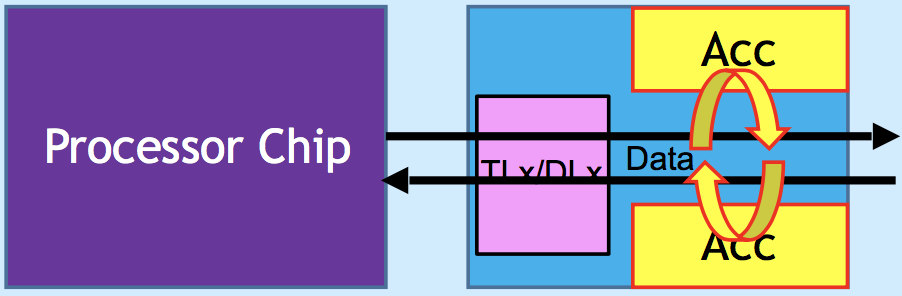
\includegraphics[width=0.45\linewidth]{2-ocapi-paradigm-5}
    \caption{Bi-directional transform.}
    \label{fig:2-ocapi-paradigm-5}
  \end{subfigure}
  \caption{Accelerator paradigms enabled by OpenCAPI \cite{opencapi-jeff-preso}.}
  \label{fig:2-ocapi-paradigm}
\end{figure}





\section{FPGA Characterization}
\label{sec:fpga-characterization}
FPGAs are integrated circuits that can be reconfigured after fabrication (field programmable). A lot can be said about FPGAs and their operation, but the focus of this section is to provide background information for those aspects of FPGAs that most directly relate to the implementation of the proposed architecture. The background information provided in this section will be used throughout the rest of the thesis.



\subsection{FPGA Architecture}
\label{sec:fpga-arch}
Typically, FPGAs consist of arrays of programmable logic blocks that can be wired together. Logic blocks can be used to implement combinatorial logic, by configuring look-up tables (LUTs), or to implement sequential logic such as flip-flops and small memories. Besides configurable blocks, also hardwired logic is present such as multiplexers, special DSP slices, networking stacks, and PCI Express controllers.\\
\autoref{fig:2-fpga-arch} shows the physical architecture of an FPGA. The most common resources such as IO Blocks, CLBs, memories, and DSP Blocks are shown. What is important to notice is that each type of resource is located in a separate column. Memories for example could be located relatively far away from where their data is processed. Depending on the target frequency of the design, wire delays could start to play a large role. When routing within a single clock cycle fails, additional registers are required between a memory and the data consumer. For this reason, memory primitives typically contain one or multiple additional pipeline stages within the primitive to help with routing, at the cost of increased latency.

\begin{figure}[H]
  \centering
  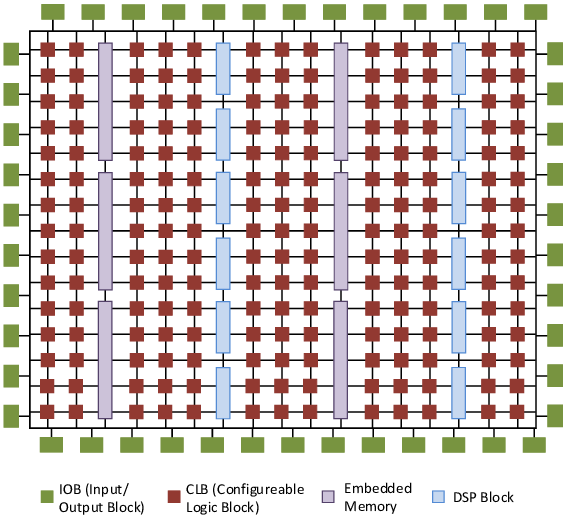
\includegraphics[width=0.50\textwidth]{2-fpga-arch.png}
  \caption{Diagram showing the physical architecture of an FPGA \cite{fpga-fig}.}
  \label{fig:2-fpga-arch}
\end{figure}



\subsection{Typical Resources}
We study two Xilinx FPGAs for their suitability to be used as OpenCAPI accelerators. Both FPGAs, the KU15P and VU37P, are from the latest UltraScale+ architecture and are the highest model in each device family, Kintex+ and Virtex+, respectively. Compared to previous architectures, UltraScale+ adds Ultra RAM (URAM). This memory resource falls in between the typical BRAM and DRAM capacities, and High Bandwidth Memory (HBM) Gen 2 for the top tier Virtex+ FPGAs. Table \ref{tab:fpga} shows a summary of specifications for both FPGAs. The GTY transceivers mentioned in the table have a maximum bandwidth of \SI{32.75}{\giga\bit\per\second}, which is more than that of the OpenCAPI lanes at \SI{25}{\giga\bit\per\second}. The table shows that both FPGAs can easily handle eight lanes to attach to OpenCAPI. The following itemization explains most of the specifications in more detail. It is important to note that the VU37P excels in every aspect compared to the KU15P.
\begin{itemize}
  \item{\textbf{CLB flip-flops} reports the number of flip-flops across all CLBs in thousands.}
  \item{\textbf{CLB LUTs} reports the number of LUTs across all CLBs in thousands.}
  \item{\textbf{Distributed RAM} reports the maximum memory capacity.}
  \item{\textbf{BRAM} reports the total memory capacity, both with and without ECC support.}
  \item{\textbf{URAM} reports the total memory capacity, both with and without ECC support.}
  \item{\textbf{HBM} reports the total available HBM capacity on the FPGA.}
  \item{\textbf{DSP slices} reports the number of available DSP slices on the FPGA.}
  \item{\textbf{GTY transceivers} reports the total number of \SI{25}{\giga\bit\per\second} transceivers available.}
\end{itemize}

\begin{table}[h]
  \centering
  \caption{Specification summary of the Xilinx KU15P and VU37P FPGAs \cite{xilinx-fpga}.}
  \label{tab:fpga}
  \begin{tabular}{ l | c | c }
    \textbf{Resource}               & \textbf{KU15P}  & \textbf{VU37P} \\ \hline
    %System logic cells (K)          & 1143            & 2852 \\
    CLB flip-flops [k]              & 1045            & 2607 \\
    CLB LUTs [k]                    & 522             & 1304 \\
    %Number of distributed RAMs      & 161280          & xxx \\
    Distributed RAM capacity [Mb]   & 9.8             & 36.7 \\ % KU15P = 161280 * 64b / 8b/B
    %Distributed RAM [Mb]            & 9.8             & 36.7 \\
    %Number of BRAMs                 & 984             & 1968 \\
    BRAM capacity with ECC [Mb]     & 34.6             & 70.9 \\ % KU15P = 512*72*984/8
    BRAM capacity without ECC [Mb]  & 30.8             & 63.0 \\ % KU15P = 512*64*984/8
    %Total block RAM [Mb]            & 34.6            & 70.9 \\
    %Number of URAMs                 & 128             & \\
    URAM capacity with ECC [Mb]     & 36.0             & 270.0 \\ % KU15P = 4*1024*72*128/8
    URAM capacity without ECC [Mb]  & 32.0             & 240.0 \\ % KU15P = 4*1024*64*128/8
    %Total ultra RAM [Mb]            & 36.0            & 270.0 \\
    HBM capacity [GB]               & 0               & 8 \\
    DSP slices                      & 1968            & 9024 \\
    GTY transceivers                & 32              & 96 \\
  \end{tabular}
\end{table}



\subsection{Configurable Logic Blocks}
\label{sec:clb}
The UltraScale+ architecture consists of an array of Configurable Logic Blocks (CLB), with two distinct flavors \cite{xilinx-ug574}. Each CLB consists of eight six-input LUTs, sixteen flip-flops, and seven hardwired multiplexers to select between LUT outputs if needed. A LUT is used to implement a logic function and each of them is accompanied by two flip-flops and can be configured as either a six-input one-output or a five-input two-output LUT. Besides the hardwired multiplexers, the LUTs can also be used to implement a 4:1 multiplexer by using four inputs for data and two inputs for the selection signal. \autoref{fig:2-xilinx-mux} shows how a 16:1 multiplexer can be implemented in half of a CLB. Similarly, a 32:1 multiplexer can be implemented in a single CLB by using all LUTs and hardwired multiplexers. Internally, a CLB can either be a \textit{SLICEL} or a \textit{SLICEM}. The previously mentioned logic is present in a \textit{SLICEL}. In addition to this, a \textit{SLICEM} can also be configured with up to \SI{512}{\bit} of distributed RAM or with a \SI{256}{\bit} shift register. Distributed RAM can be configured as single, dual, quad, octal or simple dual-port with a minimum memory capacity of \SI{32}{\bit} per primitive up to a maximum of \SI{512}{\bit} per slice with either \SI{1}{} or \SI{2}{\bit} wide data.

\begin{figure}[h]
  \centering
  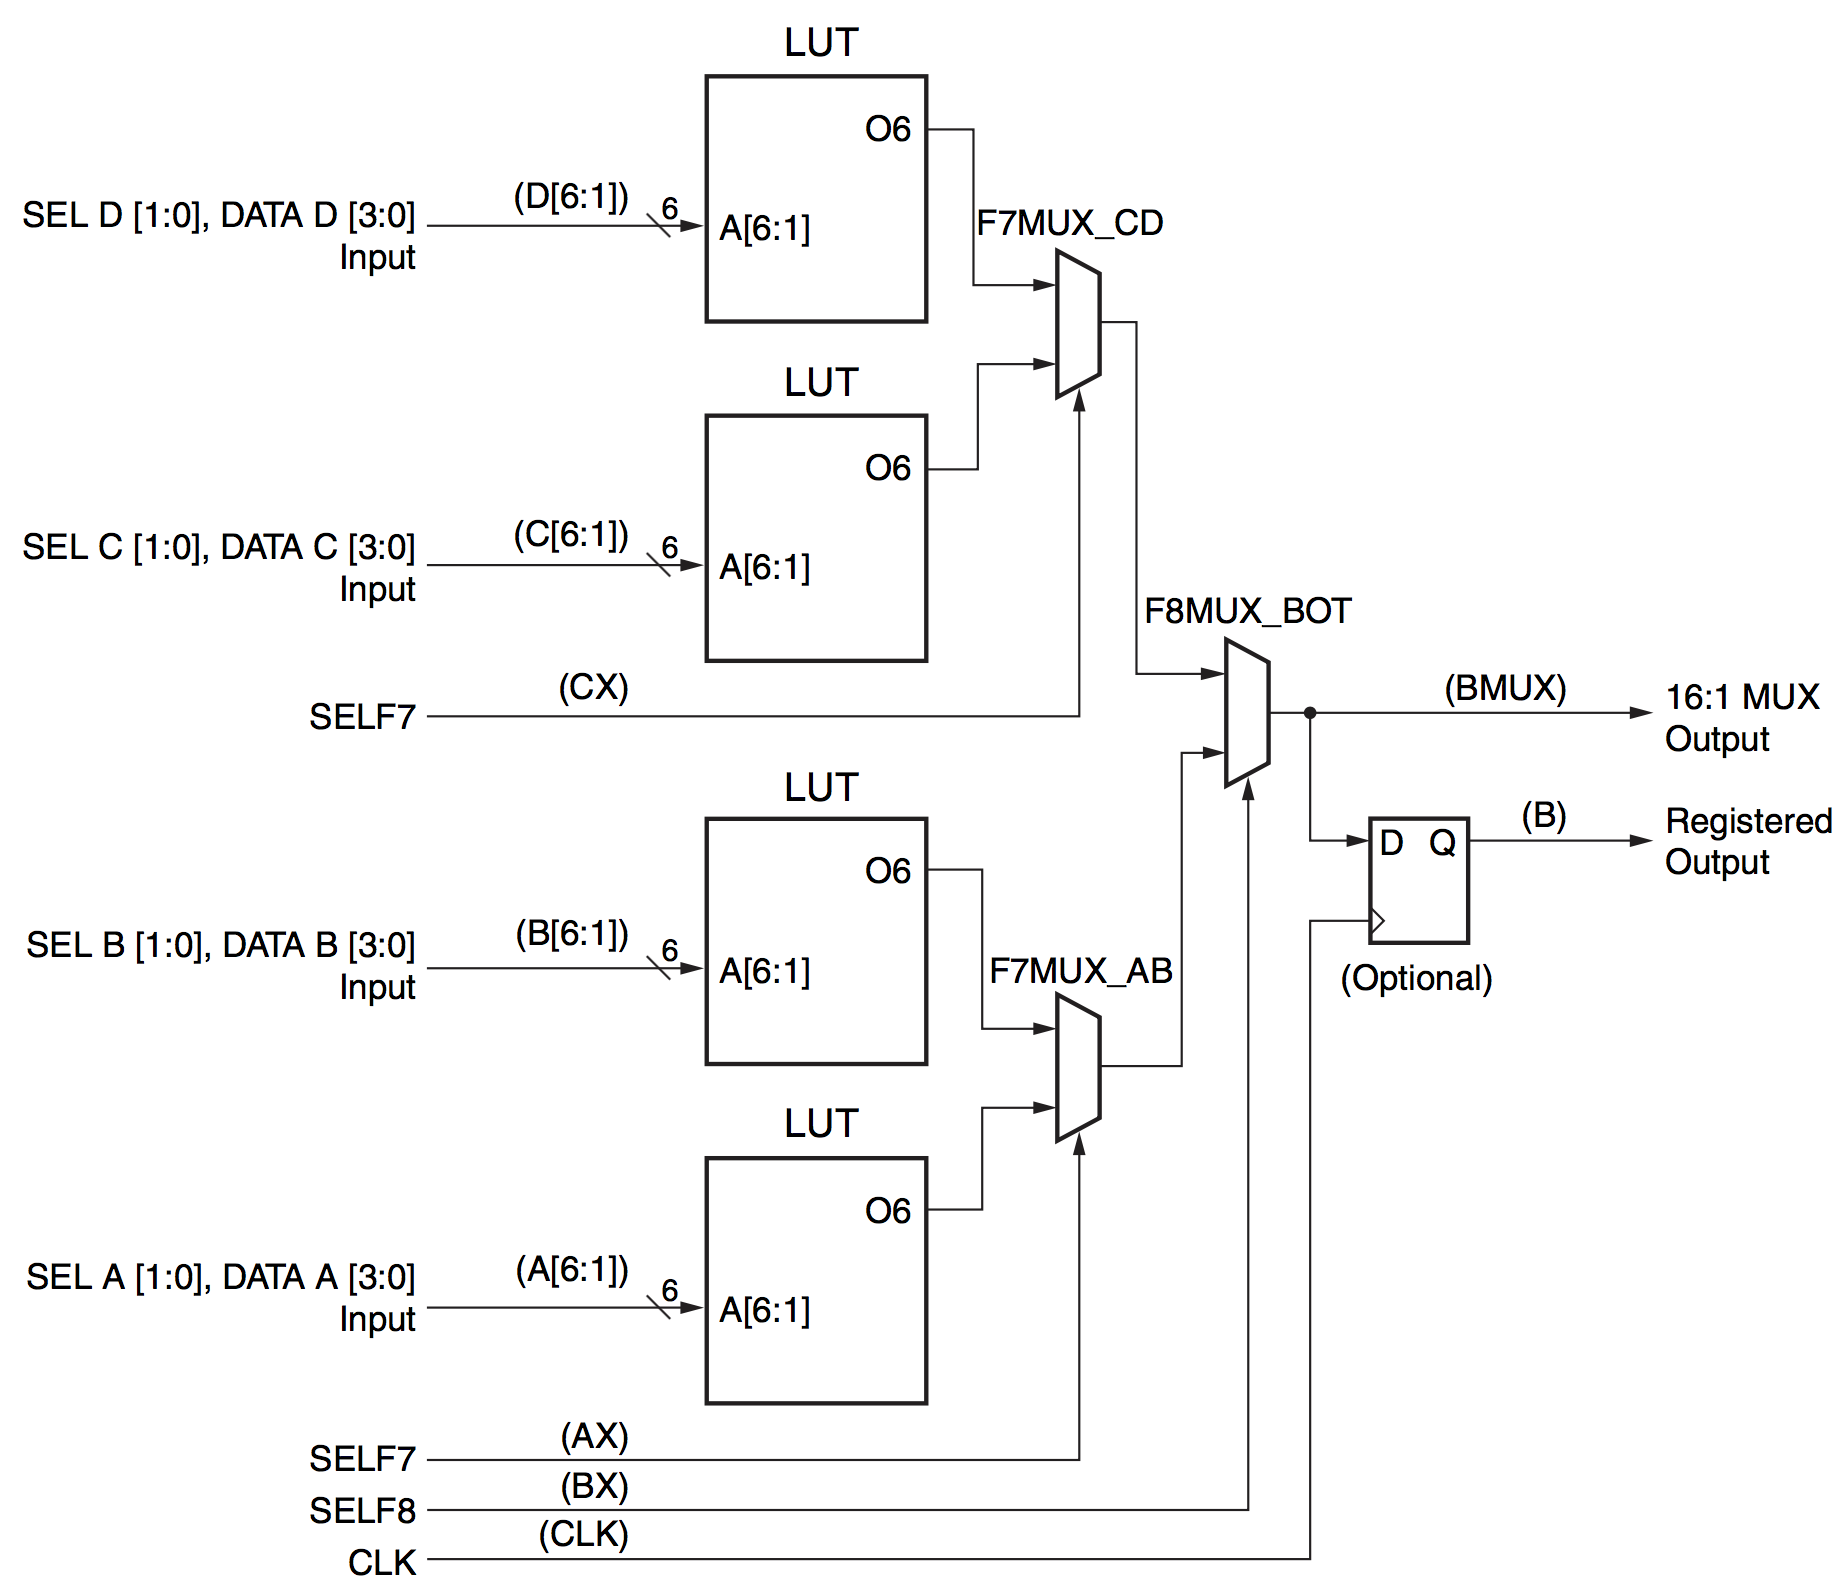
\includegraphics[width=0.70\textwidth]{2-xilinx-mux.png}
  \caption{16:1 multiplexer using half a CLB in the UltraScale+ architecture \cite{xilinx-ug574}.}
  \label{fig:2-xilinx-mux}
\end{figure}



\subsection{Memory Resources}
Several different memory resources exist, either inside or outside of the FPGA. The UltraScale+ architecture brings two additional memory resources to the table: URAM and HBM. The following list is sorted based on increasing memory capacity and latency \cite{xilinx-ug573}.
\begin{itemize}
  \item{\textbf{Distributed RAM} is RAM built from LUTs within a slice and supports several configurations. Multiple read ports are supported, but multiple write ports are not.}
  \item{\textbf{Block RAM} are dedicated RAM primitives with ECC support of \SI{36}{\kilo\bit} in size. The primitive consists of two independent \SI{18}{\kilo\bit} RAMs that can be configured as a Simple Dual Port (SDP) or True Dual Port (TDP) memory. Each BRAM has two independent read and write ports. A \SI{36}{\kilo\bit} BRAM can be configured with independent ports as 32K x 1, 16K x 2, 8K x 4, 4K x 9, 2K x 18 or 1K x 36 for a TDP configuration or additionally as 512 x 72 for an SDP configuration. An \SI{18}{\kilo\bit} BRAM can be configured with the same data widths, but with half of the entries. By default the read latency is one cycle, but an optional read register can be configured.}
  \item{\textbf{Ultra RAM} are also dedicated RAM primitives with ECC support but have a larger capacity compared to BRAM primitives. Two ports are available and one configuration of 4K x 72. A port either operates as a read or write port and port A always completes before port B does. Similarly to a BRAM primitive, optional registers can be configured between one and four cycles of latency.}
  \item{\textbf{HBM} is high-bandwidth memory reaching bandwidths up to \SI{460}{\giga\byte\per\second}. This memory is only supported on top tier Virtex+ FPGAs up to \SI{8}{\giga\byte} \cite{xilinx-hbm}.}
  \item{\textbf{DRAM} is located outside of the FPGA and has a capacity of up to several gigabytes.}
\end{itemize}

%\todo{- add max frequencies of RAMs.\\}



\subsubsection{BRAM Address Collision}
An address collision occurs when both ports of a BRAM primitive access the same address in a single clock cycle. The resulting behavior depends on the port configuration. If both ports read, both accesses complete successfully. If both ports write, the memory location contains non-deterministic data. If one port reads and the other writes, the write data operation completes successfully. The read access is only successful for common clock designs and the write port is configured as read-first \cite{xilinx-ug573}.



\subsubsection{URAM Address Collision}
Similarly, an address collision can also occur for a URAM primitive. When both ports write in the same clock cycle, the port B write takes effect since port A always completes before port B. If port A reads and port B writes, port A receives the old data and the new data is stored at the memory location. If port A writes and port B reads, the new data is written to the memory location and port B reads the new data immediately \cite{xilinx-wp477}.


%- add info about SDP and TDP BRAMs and when collisions occur. see \url{https://www.xilinx.com/support/documentation/ip_documentation/blk_mem_gen/v8_3/pg058-blk-mem-gen.pdf} page 51.\\
%- is BRAM write at most one cycle? should check or test this. according to UG573 page 12 BRAM write operation is always single clock-edge operation. Read uses one or two, depending on if the output register is configured.\\

%Xilinx PCIe Memory Bandwidth - WP464\\
%Using WP464 with 2.5 scaling factor to account for both read and write directions and any additional overhead such as memory addressing. Total memory bandwidth required for sustained transfers:
%\begin{equation}
%  $50GB/s * 2.5 = 125 GB/s = 1000 Gb/s$
%\end{equation}
%Required interface width for DDR4 memory at 2133Mb/s:
%\begin{equation}
%  $1000 Gb/s / 2133Mb/s per pin = \approx 469 pins$
%\end{equation}
%DDR4 memory is supplied in 288-pin dual in-line memory modules (DIMMs).



\subsection{DLX and TLX Reference Design}
\label{sec:dlxtlx}
As mentioned in Section \ref{sec:cacheline}, a DLX and TLX reference design is provided that can be integrated as a module by the AFU designer. Because the reference design is implemented in FPGA logic, care must be taken that both the reference design and the AFU fit inside the specific FPGA resource budgets. \autoref{tab:9v3} shows the resource utilization obtained using Vivado 2017.1 when targeting a Xilinx VU3P FPGA on the Alpha Data 9V3 OpenCAPI-capable card. The number of resources used and the percentage consumed of the total number of resources available are shown. These results are from October 10, 2017 and are subject to change \cite{opencapi-enablement}.

\begin{table}[H]
  \centering
  \caption{Resource utilization for the DLX and TLX layers \cite{opencapi-enablement}.}
  \label{tab:9v3}
  \begin{tabular}{ l | c | c | c }
    \textbf{Resource}   & \textbf{DLX}  & \textbf{TLX}  & \textbf{Total} \\ \hline
    CLB Registers       & 9392 (1.19\%) & 13806 (1.75\%)    & 23198 (2.94\%) \\
    CLB LUTs            & 19026 (4.83\%) & 8463 (2.15\%)    & 27489 (6.98\%) \\
    LUT as Memory       & 0 (0\%) & 2156 (1.09\%)           & 2156 (1.09\%) \\
    BRAMs               & 7.5 (1.0\%) & 0 (0\%)             & 7.5 (1.0\%) \\
  \end{tabular}
\end{table}

%\todo{
%- "Memcopy, Home Agent Memory and AFP exercisers are all up and running cleanly using the Alpha Data 9V3 card with VU3P FPGA"\\
%- 9V3 datasheet in comment % https://www.alpha-data.com/pdfs/adm-pcie-9v3%20user%20manual.pdf
%}
%\todo{
%I remember that ADM might be what you mean (Alpha Data). They have OpenCAPI cards for VU3P. They also said they are going to support one like VU37P.
%}

\section{Preliminary Concluding Remarks}
The bottlenecks present in the traditional IO model are addressed by OpenCAPI and this chapter provided a deeper understanding of this protocol. Additionally, various emerging use cases for attached accelerators are presented. A brief summary of the latest generation of Xilinx FPGAs, compatible with OpenCAPI, is required for the remainder of this thesis. Due to the order of magnitude increase in interconnect bandwidth, new challenge arise for AFU designers. Questions regarding the partitioning of the algorithm, concurrent usage of multiple software threads, and the design of the accelerator come to mind.\\
Another question we can ask ourselves is how the accelerator is fed with data, since no buffer or cache is present on the attached OpenCAPI device by definition. Chapter 5 generalizes across multiple common accelerator memory access patterns and proposes an architecture to keep accelerators fed with data at OpenCAPI-like bandwidths.

  \chapter{Requirements and Naive Designs}
Section \ref{sec:3compare} concluded that recent advancements in interconnect standards try to tightly couple attached devices to host processor cores at an order-of-magnitude larger bandwidths. This has serious implications for accelerator design and, more importantly, for feeding them.\\
This chapter compares common accelerator memory access patterns and tries to generalize across several streaming-like access patterns. This benefits the data feeding architecture, since it will be applicable to a wider range of accelerators. Thereafter the merge-sort database operator is used as a case study to show that naive traditional design methodologies at these bandwidths will not suffice.





\section{Accelerator Classification}
\label{sec:class}
As mentioned in Section \ref{sec:adopt}, FPGA accelerators are most commonly used for a specific class of workloads. Therefore the memory access patterns found in these workloads are limited. The following list shows the most commonly found memory access patterns of accelerators including an example application \cite{li-mem-access}.
\begin{itemize}
  \item{\textbf{Complex} accesses are considered to be more difficult than for example strided access, but still regular and known a priori. An example is a Hessian computation found in augmented reality. Image processing also uses similar access patterns.}
  \item{\textbf{Gather} accesses multiple pieces of data from non-contiguous locations in host memory. Each request consists of an absolute address and an amount of data to retrieve. This type of access often occurs for vector arithmetic.}
  \item{\textbf{Indirect array} accesses an array using a second array: $A[B[i]]$. The data for $B[i]$ is retrieved and the returned value is used to access array $A$. An example can be found in calculating a histogram in image processing.}
  \item{\textbf{Linked-list} reads an address that points to another address and so on. An example could be a network controller that handles header and payload data structures. The header contains information regarding the payload and is typically stored as a linked-list.}
  \item{\textbf{Streaming} accesses continuous chunks of data from host memory and stores it into a local buffer for processing. Examples include encryption and video processing.}
  \item{\textbf{Strided} accesses chunks of data with a fixed distance from the current address, called strides. Matrix multiplication is an example of a strided access since columns of the matrix have to be read where the stride is the row size.}
\end{itemize}

%\todo{- Add figure of different access patterns.\\
%- you could call the stream buffer an implicit DMA, since it moves data around but only in reading fashion and no explicit read commands are made. Just a start and end address in shared coherent main memory.\\
%- what kind of access do gpus or intel phi for example have/allow?\\
%- find more sources on accelerator access patterns\\
%- how is dma and our buffer connected? why did we not use a dma?\\
%}

Typically a DMA engine is used to direct memory access between the host memory, over the interconnect, and the local memory on the accelerator. A DMA enables compute to operate in parallel with memory transfers and provides data in large spatial-continuous blocks of memory to the accelerator. From this list, it becomes apparent that only streaming access directly benefits from a typical DMA transfer. The other access patterns do not, since they require either spatial-continuous data from multiple starting addresses or a single element from multiple starting addresses. For the first case, multiple DMA transfers have to be issued sequentially or a scatter-gather engine could be used, where a list of transfers is provided. The latter case requires buffering, since transferring data element-wise is inefficient over the interconnect due to under-utilization of the available data bus. The complex access for example, would even benefit from less than a cache line\footnotemark~granularity of data. For the complex access, element granularity is preferred, where an element is the data size of a single piece of meaningful data. In the image processing example, the data of a single pixel. Element granularity access is not supported by current frameworks such as the Streaming Framework or SNAP, discussed in Section \ref{sec:capi-1.0}.\\
However, a generalization across several streaming-like access patterns can be made. This renders the buffer architecture applicable to multiple access patterns and takes it out of the design process of an AFU designer. While the three database operators mention in Section \ref{sec:aim} are streaming based, a smaller granularity allows for more flexibility, especially with other access patterns in mind. Streaming access is the simplest pattern, because spatial-continuous data is read from a single starting address. A similar pattern is the strided access because in essence it consists of multiple stream accesses at the same time, where the starting addresses are at equidistant. A generalization of the strided access is the gather access, where also multiple non-spatial-continuous locations in memory are read. However, the starting addresses do not necessarily have to be equidistant. Finally, the complex but regular access is a generalization across all of the previous patterns. It could require element-sized data from multiple memory locations at the same time. A buffer architecture with element-wise access enables, for example, the Hessian matrix complex access case. Each pixel required for the computation is located in a separate stream buffer, after which the accelerator is able to access each stream at any point in time.\\

\footnotetext{The data size transferred between the last level cache and host memory.}

As mentioned in Chapter \ref{sec:intro}, other students are studying three different accelerators for database operators: decompress-filter, hash-join, and merge-sort. In essence, each accelerator requires streaming access, but in different ways. The decompress-filter operator decompresses incoming compressed Parquet files and applies a certain filter to it. This accelerator exhibits perfect streaming access behavior. The merge-sort operator merges multiple pre-sorted key-value pair streams from main memory and merges them into a single sorted output stream. In the case of the hash join, while hash table accesses are irregular, an efficient implementation of hash-join will hold the hash tables in local memory such that the accesses to host memory are predominantly streaming.

%\todo{
%- Have to make the following bullet clear somewhere. Why do you not use a DMA or SG instead?\\
%- assess memory access of the three operators. use following link from Jian\\
%I just read an interesting paper from FPGA'16 named 'A Study of Pointer-Chasing Performance on Shared-Memory Processor-FPGA Systems'. I guess this would be a part of hash-join's memory access pattern. I am not sure whether this is useful for you. For quickly have a view of this paper, it studies a linked list traversal behavior on the shared-memory heterogeneous computer systems (CPU+FPGA) including Xilinx Zynq, Intel QuickAssist QPI FPGA Platform, and Convey HC-2EX. It points out that memory latency is an important impact for pointer-based applications and shows the potentials of using this kind of FPGA-CPU shared-memory architecture.\\
%}





\section{Merge-Sort Accelerator Case Study}
%\todo{
%- Why is cache useful? Answer: fpga has small memory. partitioning your problem for fpga, you have to keep in mind this memory limitation. since small memory requirement, the problem gets cache friendly.\\
%- memory latency for cpu is much lower than for afu. however afu runs slower so more latency is not a problem.\\
%- concern Andrew Martin about a cache for streaming applications in general. Why not use ’a shit ton of’ buffering instead to cover the latency instead of using a cache? That is what he did when building a sorter on an FPGA. Peter’s response: we try to generalize the shit ton of buffering, so basically taking it out of the design process of the AFU designer. our cache is basically a big buffer.\\
%}
%\todo{
%- mention also HBM (8GB for VU37P) as an advancement which makes heterogenous computing more interesting for memory bound problems.\\
%- Peter: "Nice aspect of sort is that it plays at all different levels of the system." Why is that the case?!\\
%}

The merge-sort operator is an interesting database operator since it inherently uses multiple streams of key-value pair data from host memory. The complexity of the operator comes from the merging of multiple streams, where the next chosen stream to read is unpredictable. For databases, key-value pairs are a common data type. A key is a unique identifier with a size of 8 bytes for example. Most important for the key size is that it is large enough such that no collisions will occur. The value could be actual data or a pointer to the actual data. Since the value could be a pointer, 8 bytes are sufficient to hold a 64 bit address. Combining both the key and value size results in a 16 byte key-value pair, referred to from now on as an element, and is the smallest amount of meaningful data.\\
As mentioned in Section \ref{sec:cacheline}, the cache line size for the POWER architecture is 128 bytes. This means that each cache line holds eight of such elements. A reasonable, but extreme, use case for a merge-sort operator would be to assume a system with 1TB of host memory capacity. The latest generation of Xilinx FPGAs support up to \SI{8}{\giga\byte} of HBM (or RAM, but our goal in this thesis is to keep up with the OpenCAPI bandwidth rather than HBM bandwidth). In order to merge-sort all pre-sorted streams in one pass, a total of 128 streams are needed. Sustaining throughput is difficult when using a single stream. The inherent requirement of multiple streams makes it easier to fully utilize the interconnect bandwidth since requests can be made concurrently. For example, in the scenario where eight elements from different streams are requested, a typical cache line granularity interface has to fetch eight cache line granularity data blocks, select the requested element from each cache line, and buffer or discard the rest. By using read ports with element granularity, no data is wasted.



\subsection{Naive Buffer Design}
\label{sec:naive-design}
Usually a buffer is placed between the incoming data interface and the data consumer (accelerator) since the availability and consumption of data may happen at different rates. A buffer is also used to hide the latency of the interconnect by placing the data close to the consumer. Since the addresses of all cache lines are known \textit{a priori} for the streaming and the streaming-like patterns discussed before, the cache lines can be easily pre-fetched to keep the buffers filled without having to flush the buffers since no data is fetched speculatively.\\
In order for the accelerator to keep up with the OpenCAPI bandwidth, it has to consume 128 bytes (cache line size) per cycle. The interface provided by the TLX to the AFU designer consists of 64 byte data buses, operating at \SI{400}{\mega\hertz}, over which 64, 128 or 256 bytes of data are transferred (taking one, two or four cycles, respectively). Since a cache line is 128 bytes in the POWER architecture, transferring less than that seems wasteful. When 64 bytes of data are requested for example, the CAPP fetches the requested 128 byte cache line and invalidates one half and transmits the other.\\
OpenCAPI supplies 64 bytes per cycle at \SI{400}{\mega\hertz} while a realistic target frequency for an accelerator is \SI{200}{\mega\hertz}. To cover an interconnect latency of \SI{1}{\micro\second} per stream (see Section \ref{sec:buffer-depth} for a more detailed explanation), 200 cache lines, or 256 when rounded up to the nearest power of two, have to be buffered on the FPGA per stream. Due to the unpredictable access pattern of the merge-sort, each stream has to be able to be read, thus have its own buffer, in any given cycle. The total buffer size \textit{B} for such an architecture can be calculated as shown in Equation \ref{eq:bbb}.
\begin{equation}
  B = N \times C \times L \implies 128 \times 128 \times 256 = \SI{4}{\mega\byte}, \text{where}
  \label{eq:bbb}
\end{equation}
\begin{itemize}
  \item{\textit{N} is the number of streams,}
  \item{\textit{C} is the cache line size in bytes, and}
  \item{\textit{L} is the latency to be covered for OpenCAPI (rounded up to the nearest power of two).}
\end{itemize}

As shown in Section \ref{sec:fpga-characterization}, the Xilinx FPGA from the Kintex+ product line has a BRAM capacity of \SI{4}{\mega\byte} and a URAM capacity of \SI{4.2}{\mega\byte}. This means that all BRAM or URAM resources are consumed by this naive buffer architecture, leaving no resources for additional control, and more importantly, the actual AFU. Both \textit{N} and \textit{L} in this equation are subject to change and pose a trade-off. Either have fewer streams or buffer fewer cache lines per stream. Fewer streams may not be problematic, depending on the application. Buffering less per stream means that for a worst-case latency scenario, the AFU has to stall since there is no meaningful data present in the buffer. This might not be a problem if the access pattern of the respective AFU is evenly distributed across all available streams (as is the case for the decompress-filter). However, in the case of the merge-sort, the access pattern is unpredictable across streams. In order to maintain the OpenCAPI throughput and support the worst-case, the number of streams is reduced to 64. This configuration consumes roughly half of all the available BRAM resources instead of all of them.



\subsection{Crossing the Cache Line Boundary}
\label{sec:boundary}
As previously mentioned, each cache line consists of eight key-value pairs or elements. Due to the absence of a cache or buffer in OpenCAPI 3.0, multiple smaller than cache line data granularity read ports are desired and would make the buffer architecture also more general. A cache would be nice but is difficult to keep coherent in the current state of OpenCAPI 3.0. Relying on software is expensive and results in overhead and increased latency. Because streaming-like patterns are targeted, a buffer is sufficient. In the future, the buffer could be extended to a cache.\\
In order to accommodate element-wise read granularity, the buffer has to have eight read ports to consume a cache line size of data every cycle. Each read port has to be able to supply an element from any of the available streams. Due to the nature of streaming access, the next read from a stream is always the next element. In essence there are four particular access patterns, shown in \autoref{fig:3-afu-access}, that are interesting to explore, since the buffer architecture has to be able to handle those access patterns. In this figure, each numbered block represents an element in a cache line. The number represents the offset within the cache line and if the element is green, the element is being read in order to show the access pattern.
\begin{itemize}
  \item{\autoref{fig:3-afu-access-1} shows the entire current cache line being read for a single stream. In this case, a single stream and cache line are being read.}
  \item{\autoref{fig:3-afu-access-2} shows the current cache line being read for eight different streams, each reading the next element at the respective offset per stream. In this case, eight different cache lines and therefore eight different cache lines are being read.}
  \item{\autoref{fig:3-afu-access-3} shows the current and next cache line being read, crossing the cache line boundary. Crossing a boundary implies that at any given moment from any stream, two consecutive cache lines have to be read in the same cycle. In this case, a single stream from which two cache lines are being read.}
  \item{\autoref{fig:3-afu-access-4} shows the worst case scenario. If four boundaries are crossed in a single cycle, four different streams and eight different cache lines must be read concurrently.}
\end{itemize}

% https://tex.stackexchange.com/questions/196481/problem-on-subfigure-2x2
\begin{figure}[H]
  \centering
  \begin{subfigure}[b]{0.475\textwidth}
    \centering
    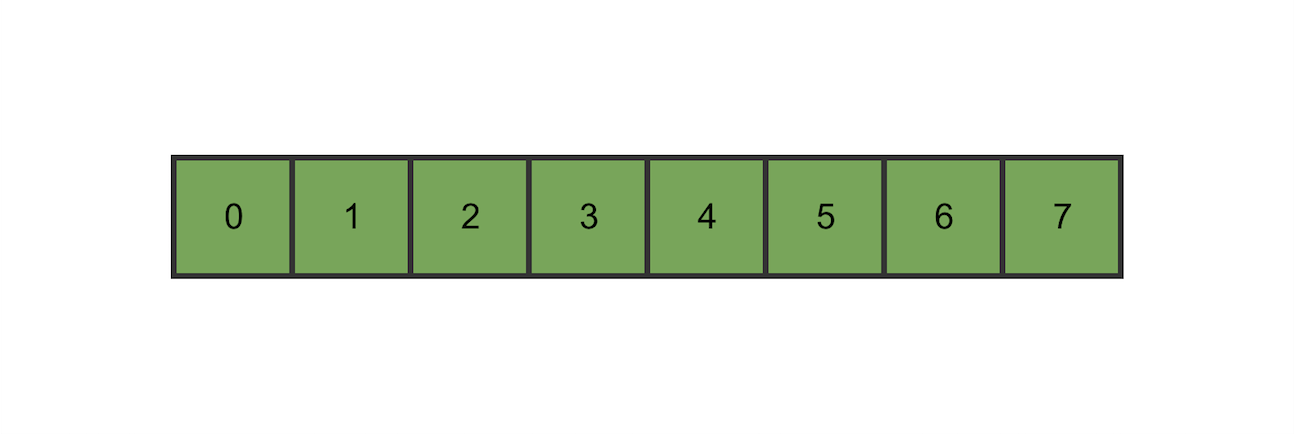
\includegraphics[width=\textwidth]{3-cross-boundary-1.png}
    \caption{Eight reads from a single stream.}
    \label{fig:3-afu-access-1}
  \end{subfigure}
  \hfill
  \begin{subfigure}[b]{0.475\textwidth}
    \centering
    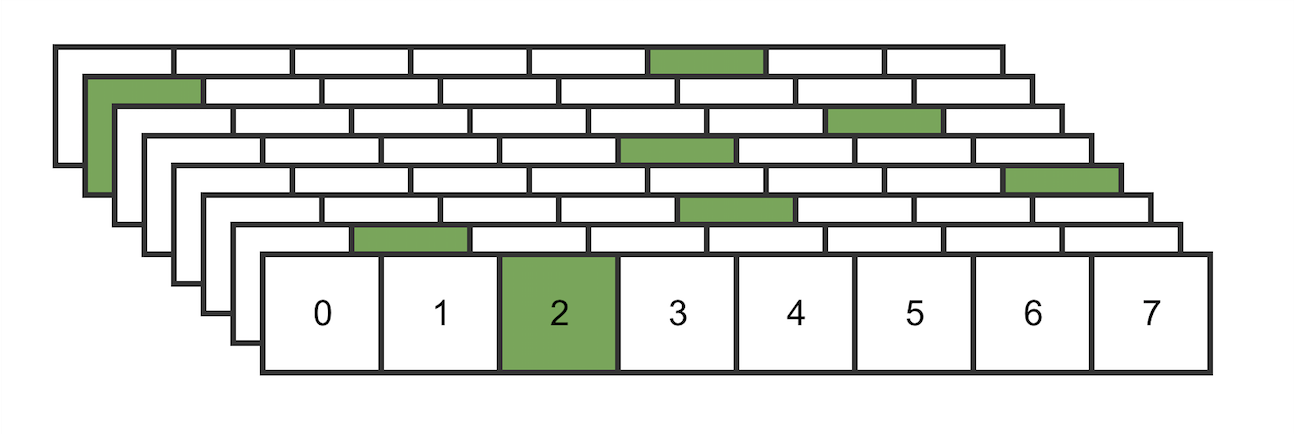
\includegraphics[width=\textwidth]{3-cross-boundary-2.png}
    \caption{Eight reads from eight different streams.}
    \label{fig:3-afu-access-2}
  \end{subfigure}
  \vskip\baselineskip
  \begin{subfigure}[b]{0.475\textwidth}
    \centering
    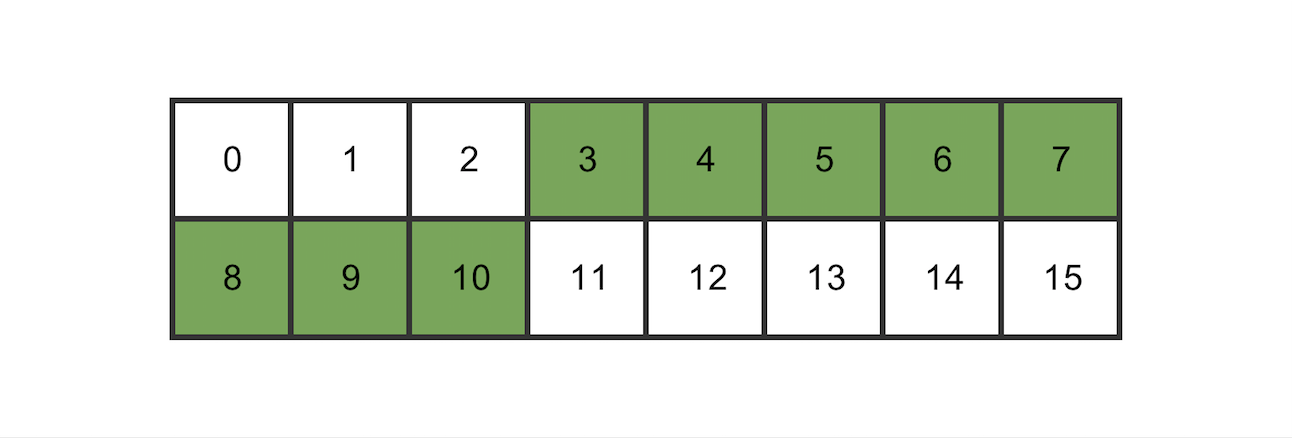
\includegraphics[width=\textwidth]{3-cross-boundary-3.png}
    \caption{Crossing a cache line boundary.}
    \label{fig:3-afu-access-3}
  \end{subfigure}
  \quad
  \begin{subfigure}[b]{0.475\textwidth}
    \centering
    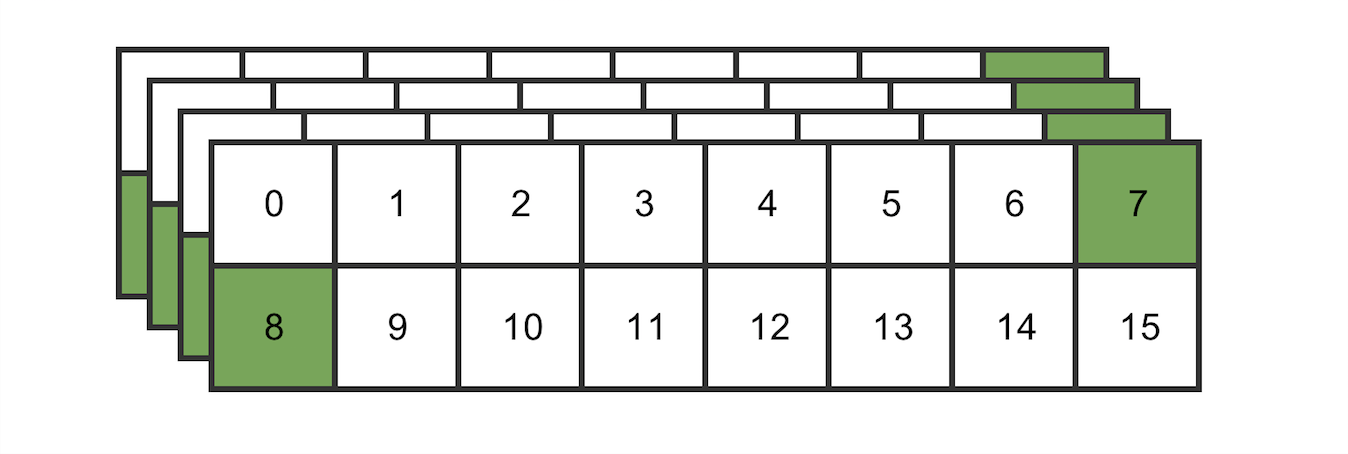
\includegraphics[width=\textwidth]{3-cross-boundary-4.png}
    \caption{Crossing four cache line boundaries.}
    \label{fig:3-afu-access-4}
  \end{subfigure}
  \caption{Four AFU access patterns using an eight read port buffer.}
  \label{fig:3-afu-access}
\end{figure}

Internally increasing the cache line size will not solve the problem of crossing cache line boundaries because the new boundary can also be crossed at some point. In essence, besides requiring a large memory to buffer the proper number of cache lines per stream, an eight read port memory is required with the granularity of a single element. This problem becomes less complex if the eight read ports would be constrained in a certain way. For example, by dividing the number of streams by the number of read ports and have each read port be dedicated to a subset of the streams. However, this contradicts the desire to keep up with the high-bandwidth and low latency interface provided by OpenCAPI. For unpredictable access patterns across streams, certain read ports may have nothing to do because of such a constraint. It also limits the access pattern generalization to not exclusively support purely streaming accesses.





\section{Design Requirements}
\label{sec:reqs}
It has become clear that a buffer architecture is needed for accelerators with streaming access patterns for which we wish to fully utilize the high-bandwidth and low latency interface of OpenCAPI. In order to do so, an access pattern generalization has been made that requires multiple read ports to concurrently and independently read from multiple independent streams of data. The merge-sort case study showed that a first-order naive design approach is not able to solve this problem and that care must be taken in order to maintain the design philosophy of high-bandwidth and low latency memory access for FPGA accelerators. Based on the previous chapters, the following is a set of requirements to which the final design has to comply in order to achieve these goals.

\begin{itemize}
  \item{Buffer 64 different streams in order to sustain the high bandwidth of OpenCAPI.}
  \item{Cover the OpenCAPI latency of \SI{1}{\micro\second} per stream.}
  \item{Go from 128 byte read port granularity to 16 byte data element granularity.}
  \item{Provide eight individual read ports such that if one read port cannot continue, the rest can still make progress.}
  \item{Handle reading across multiple cache line boundaries in a single cycle.}
  \item{Provide read ports with a low-latency between read request and data response.}
  \item{Provide a simple AFU interface by requesting data elements using stream identifiers. Streams are initially functionally reset such that an AFU has no knowledge of the addresses used.}
  \item{Provide a simple but generic interconnect interface that can be bridged to any current or future interconnect standard.}
  \item{Target the KU15P FPGA since the design can be scaled to fit the VU37P. Especially due to the vast increase in number of GTY transceivers, multiple OpenCAPI bricks can be attached.}
  \item{Confirm that the reference DLX and TLX design, provided by the OpenPOWER Foundation, also fits on the FPGA.}
  %\item{What kind of interface will I provide to the AFU designer? AXI (stream)?}
  %\item{Extendable in the future to a cache.}
\end{itemize}

%Work Element Descriptor (WED):\\
%- how will the WED look like, will there be a job queue or just a MMIO space on the AFU which holds the address in main memory of the job for each thread (context).\\
%- work element descriptor, what will it look like in a general case?\\
%- How does FU interact with memory? Does wed.source contain all information or is the AFU able to operate autonomously? Depends on application, some use WED work queue, others keep on sending WEDs instead.\\
%- support multiple engines in my framework. that means using and generating AFUTags (from the top of my head)\\





\section{Naive Design Exploration}
Section \ref{sec:naive-design} showed that a traditional approach of placing a buffer between the OpenCAPI interface and the accelerator for each stream will not fit on the target FPGA. The additional problem is the possibility of reading across a cache line boundary as shown in Section \ref{sec:boundary}. While the number of streams, the number of cache lines buffered per stream, or both can be reduced, the difficulty at hand is the required eight individual read ports with access to two consecutive cache lines in every stream buffer. This problem can be generalized as an eight read-port memory. Since FPGAs do not have the same level of flexibility as an ASIC has in terms of custom multi-ported memory cells, a solution has to be found regarding the available memory primitives. There are several traditional memory organizations that enable multi-port read access, built from smaller memory primitives.

\begin{itemize}
  \item{\textbf{Banked Memory} divides the total memory capacity into smaller memories called banks. Read requests are distributed across the banks. If multiple requests require access to the same bank, arbitration is required.}
  \item{\textbf{Duplication} replicates the memory contents in multiple memories and divides the read ports among them. Care has to be taken in order to keep the memories synchronized. Either by writing to all memories simultaneously or by keeping a live value table that keeps track of where valid data is located.}
  \item{\textbf{Multi-pumping} enables sharing of a common resource by running part of the logic at a multiple of the global frequency. For example, a memory primitive can be run at twice the frequency, effectively doubling the read ports or the data width.}
  %\item{\textbf{Rotating Buffer} provides a single buffer interface to all read ports where the oldest data gets rotated out, the other data shifts and new data gets rotated in.}
  \item{\textbf{Multi-port Primitives} provide multiple ports to the same memory. Since the target device is an FPGA, custom cells are not an option, but BRAMs can be configured as a true dual port primitive for example.}
\end{itemize}

%\todo{
%- make sure that for each BRAM limited example, also the 18kb example is mentioned, which is just a 36kb BRAM but with half the data width.\\
%- When calculating the estimated sizes of MUX structures and number of BRAMs, include the calculations as an appendix.\\
%}




\subsection{Cache Line Interleaving}
For each stream buffer, both cache line \textit{N} and \textit{N+1} could be read in the same cycle, as illustrated in \autoref{fig:3-afu-access-3}. This can be achieved by using a banked memory organization and interleaving even and odd cache lines, as shown in \autoref{fig:3-interleave-1}. Each bank consists of half of the total number of cache lines per stream and is built from multiple BRAM primitives as shown in \autoref{fig:3-interleave-2}. BRAMs are chosen because there is not enough distributed RAM available. URAMs have a fixed configuration of 4096 entries. This is too large for a single bank and the access latency of DRAM is too high. Each BRAM is configured as a 512 entry, \SI{8}{\byte} wide memory, of which sixteen are needed per bank. Basically each BRAM holds half of a \SI{16}{\byte} element, where the element offset is denoted by the numbers zero through seven and each half is denoted by suffix \textit{a} or \textit{b}. The green box shows how a single element is divided between two BRAM primitives and each half is located at address zero. The entire cache line is spread horizontally across BRAM primitives and can be accessed by reading at the same address in all sixteen BRAMs simultaneously. Doing this in both banks yields two successive \SI{128}{\byte} cache lines from which a single \SI{16}{\byte} element has to be selected by means of a \SI{256}{\byte}:\SI{16}{\byte} multiplexer for each read port. This architecture works under the assumption of a streaming access pattern because only successive elements are read. In a single cycle, only elements in two consecutive cache lines can be read. Therefore, each bank does not have to have eight physical read ports, but the requested element can be read by selection. While this architecture works in theory, there are two distinct drawbacks: multiplexer logic and BRAM primitive usage.

%\begin{figure}[H]
%  \centering
%  \begin{subfigure}[c]{.5\textwidth}
%    \centering
%    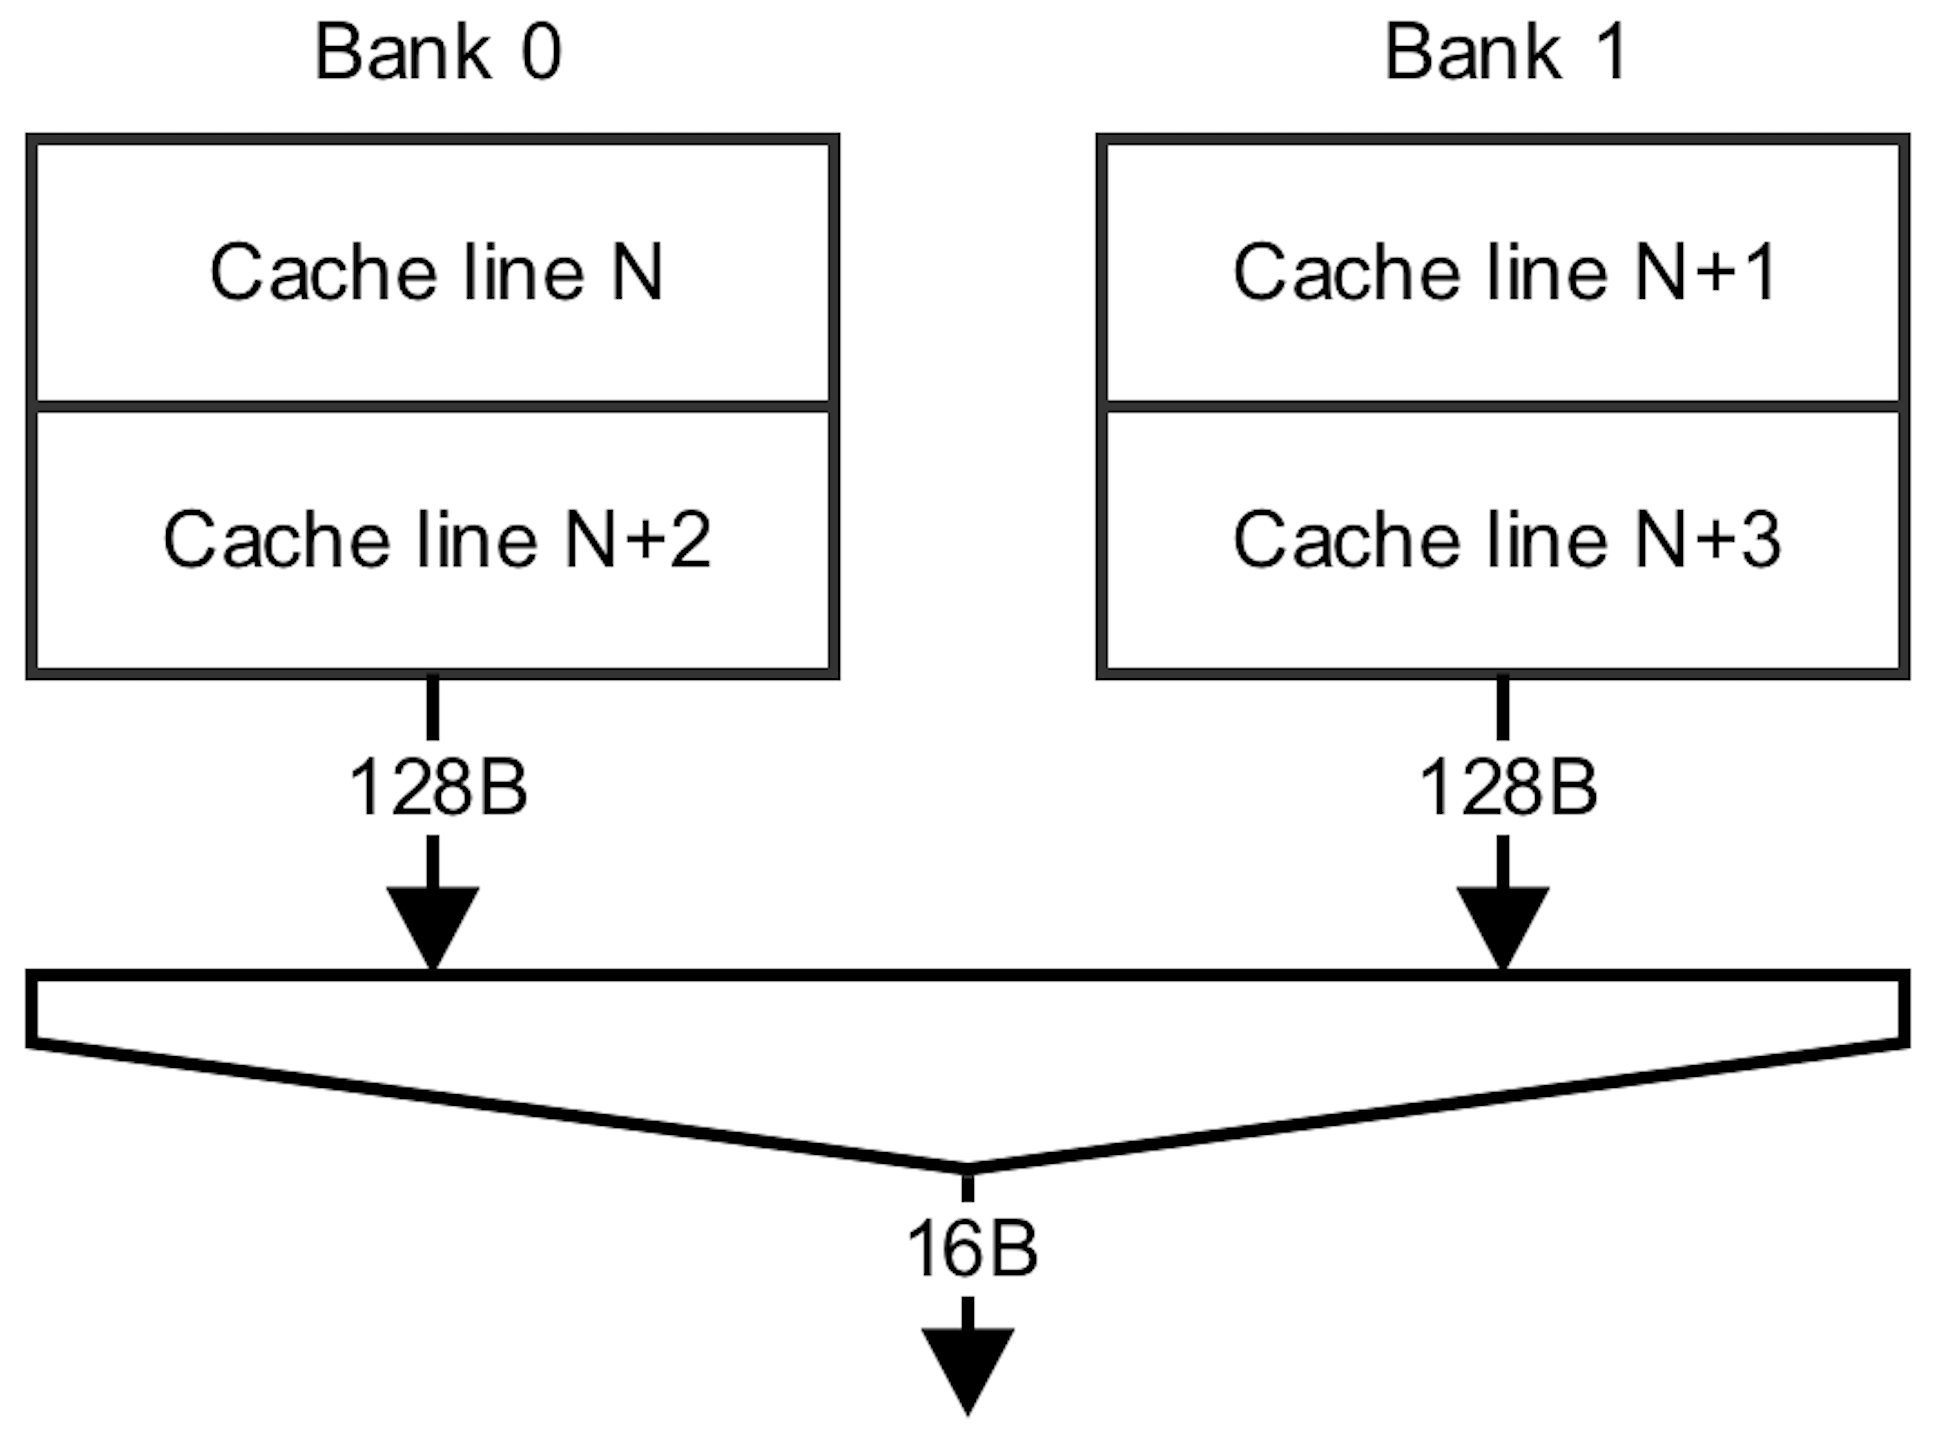
\includegraphics[width=0.7\linewidth]{3-interleave-1.png}
%    \caption{Two cache line banks per stream buffer.}
%    \label{fig:3-interleave-1}
%  \end{subfigure}%
%  \begin{subfigure}[c]{.5\textwidth}
%    \centering
%    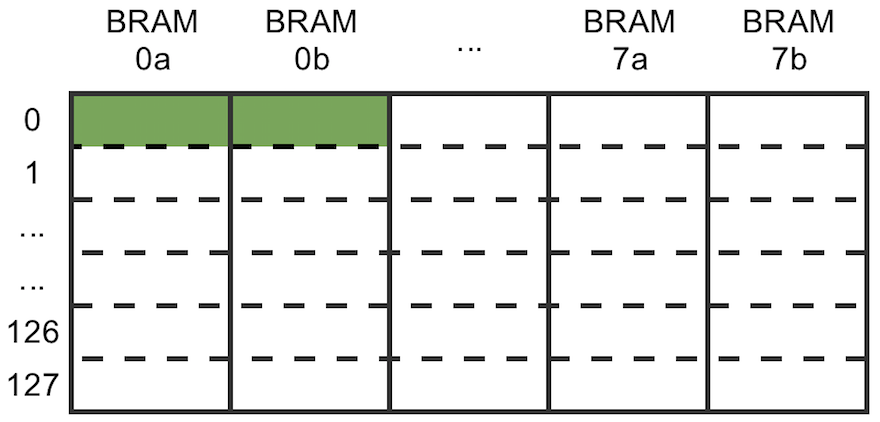
\includegraphics[width=0.8\linewidth]{3-interleave-2a.png}
%    \caption{Memory organization of a single bank.}
%    \label{fig:3-interleave-2}
%  \end{subfigure}
%  \caption{Interleaving even and odd cache lines.}
%  \label{fig:3-interleave}
%\end{figure}

\begin{figure}[htb!]
\ffigbox[\textwidth]
  {
    \begin{floatrow}
    \ffigbox[\linewidth]
      {\captionof{subfigure}{Two cache line banks per stream buffer.}
      \label{fig:3-interleave-1}}
      {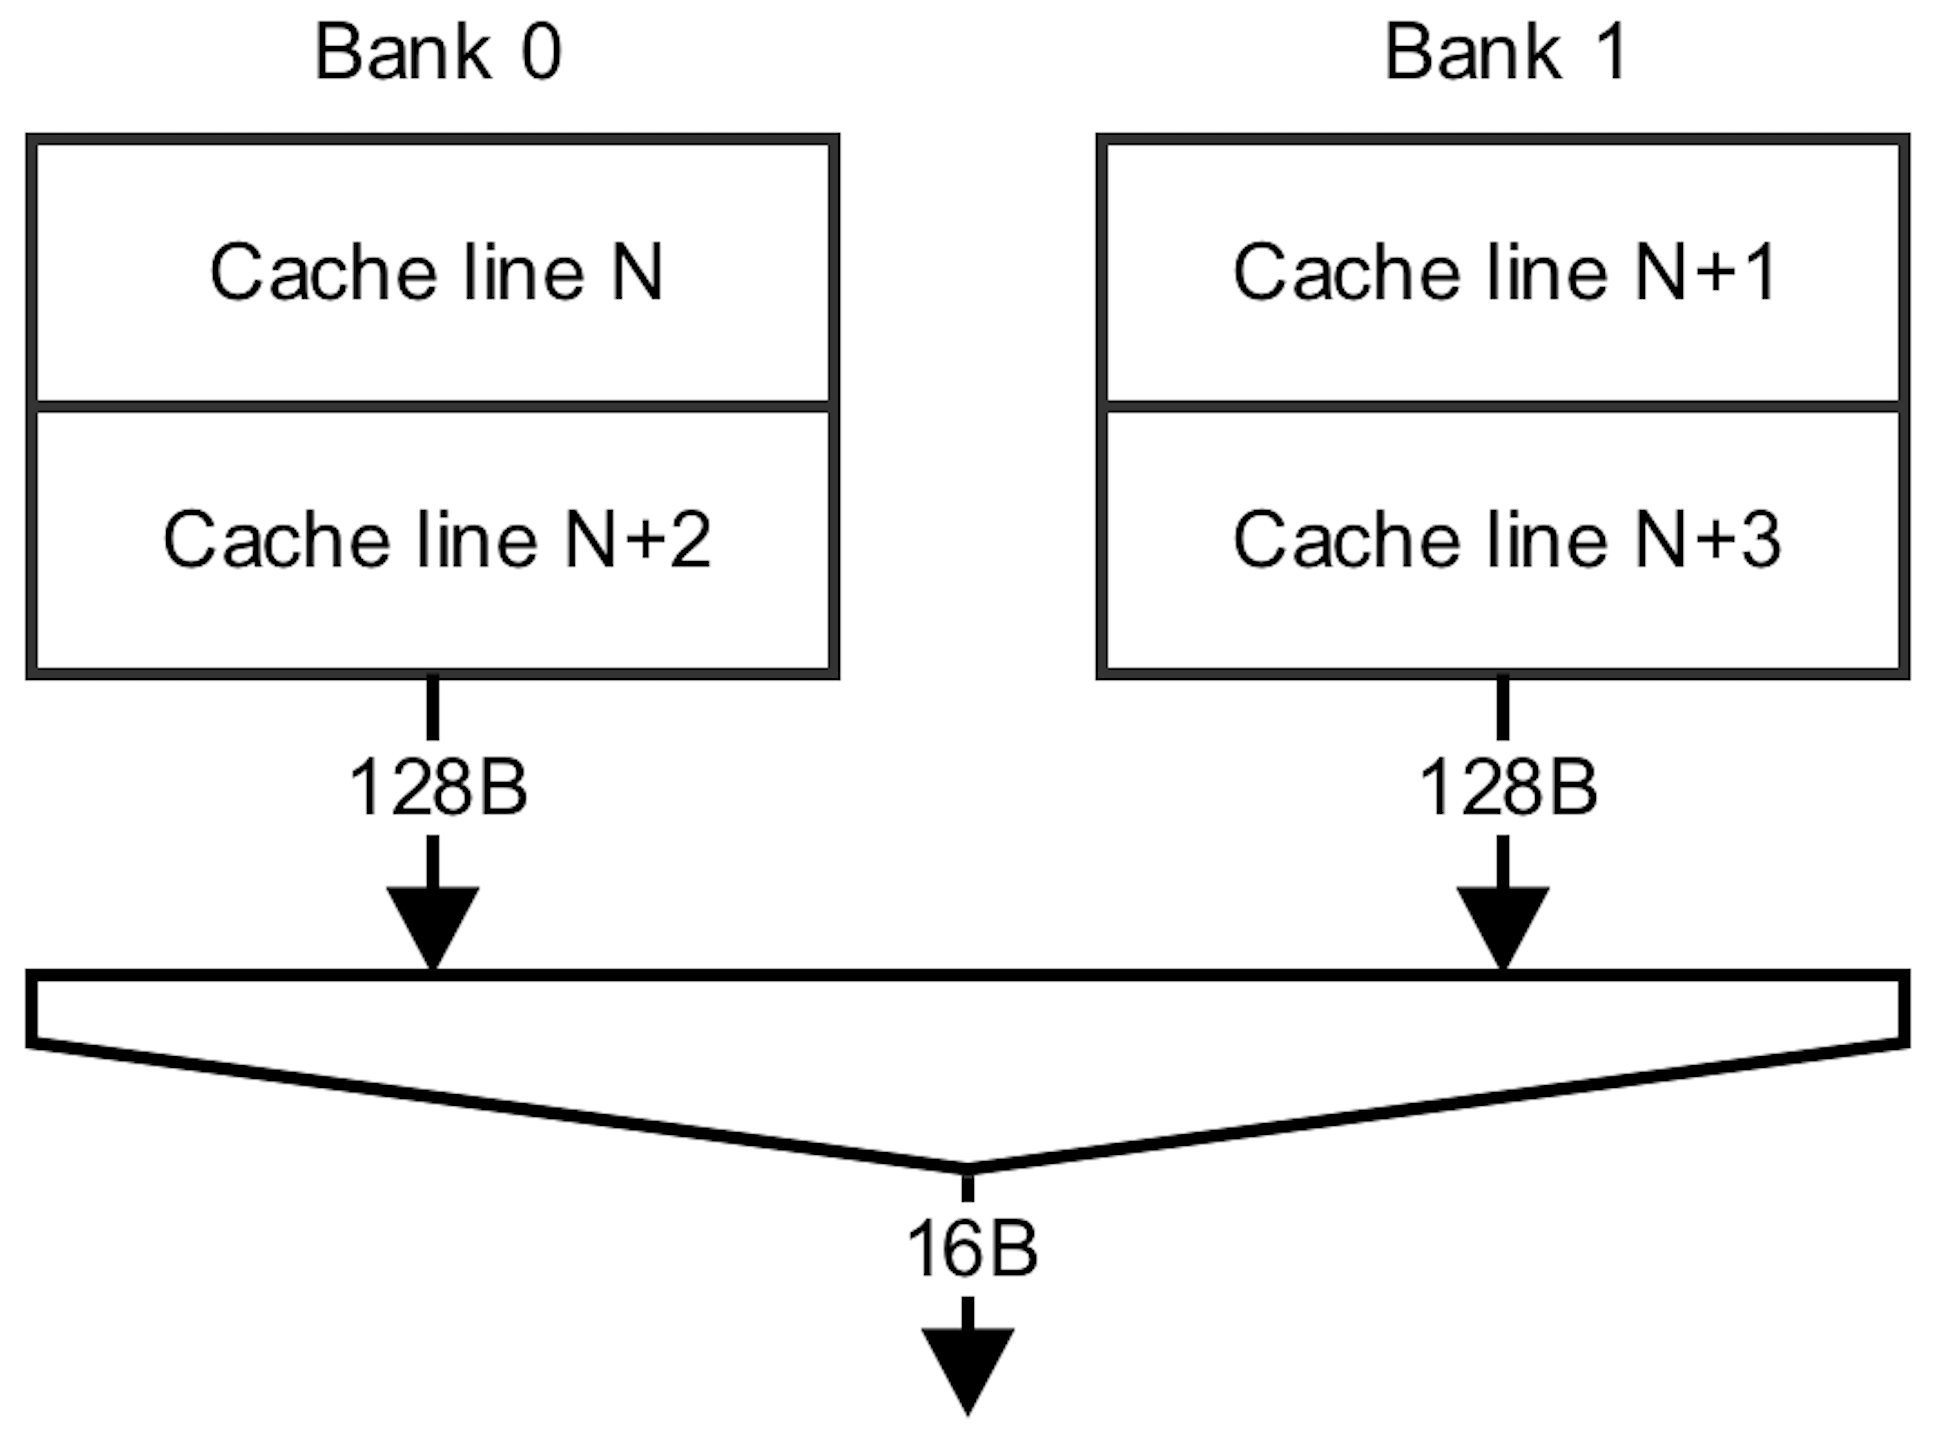
\includegraphics[width=0.80\linewidth]{3-interleave-1.png}}
    \ffigbox[\linewidth]
      {\captionof{subfigure}{Memory organization of a single bank.}
      \label{fig:3-interleave-2}}
      {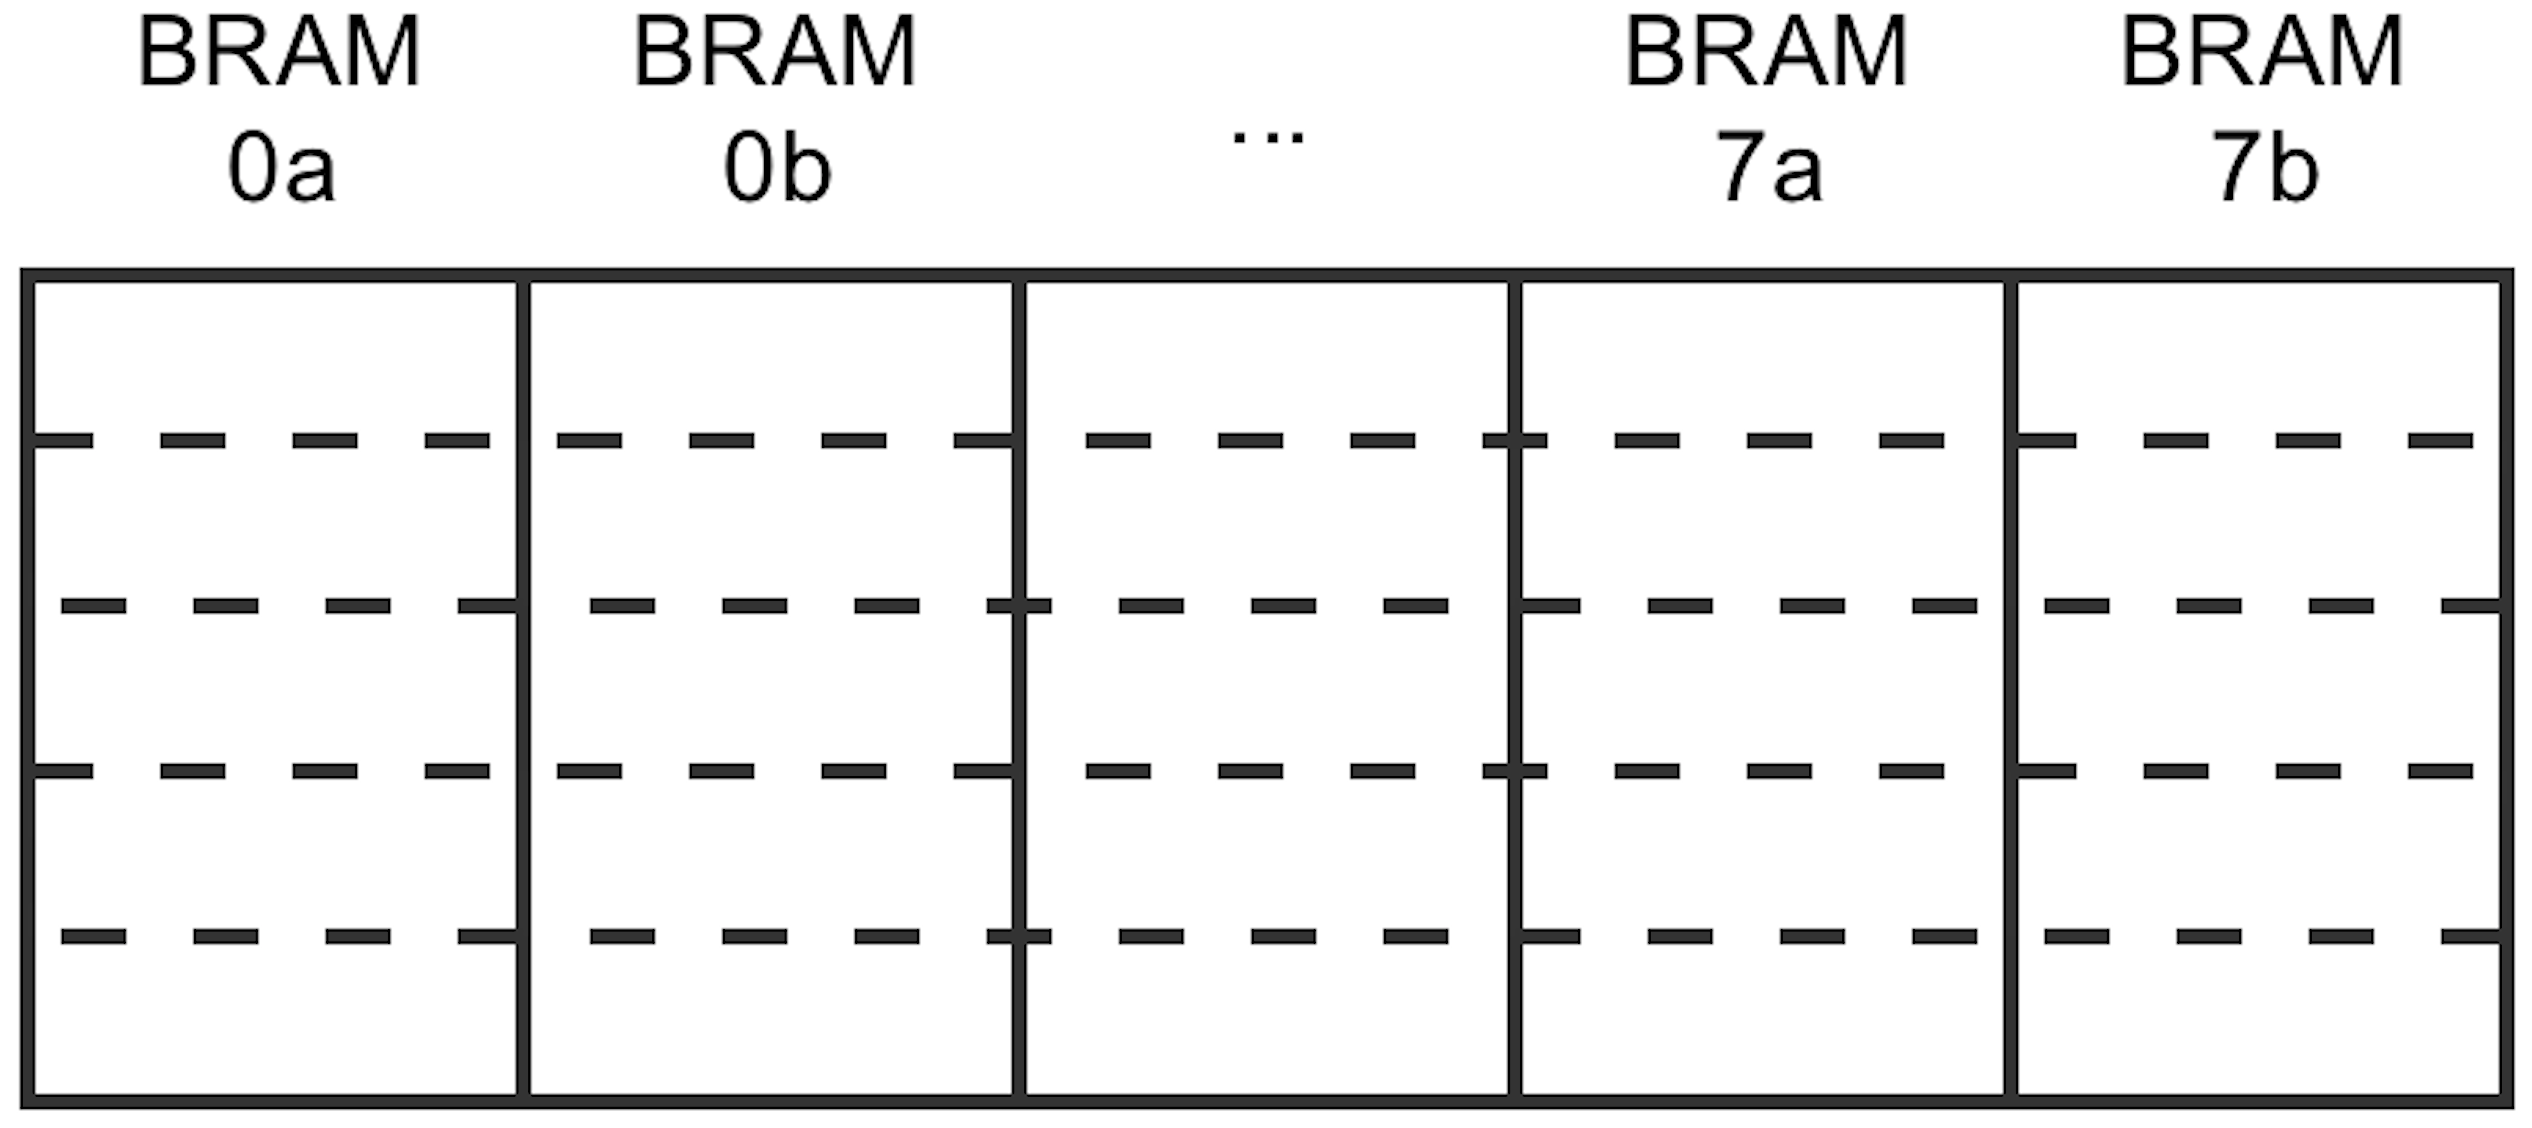
\includegraphics[width=0.80\linewidth]{3-interleave-2.png}}
    \end{floatrow}%
  }
  {\caption{Interleaving even and odd cache lines.}\label{fig:3-interleave}}
\end{figure}



\subsubsection{Multiplexer Logic}
In order to extract the correct \SI{16}{\byte} element from these two cache lines, the correct cache line (2:1 MUX) and the correct element (8:1 MUX) have to be selected. Since any read port can access any stream, the correct stream has to be selected, adding an additional 64:1 multiplexer. In total, each read port requires a 1024:1 multiplexer per bit of an element, resulting in 128 (16 bytes is 128 bits) of these multiplexers per read port.\\
Table \ref{tab:mux} summarizes several configurations of multiplexers after synthesis in the Xilinx Vivado 2017.1 tools targeting the KU15P. The column denoted by \textit{Ways} is the number of selectable inputs and \textit{Width} is the width in bits of each of those inputs. The estimation of the number of LUTs is based on the multiplex structures discussed in Section \ref{sec:clb}. Multiplexing of 32 or fewer inputs can be done within a single CLB. \autoref{fig:2-xilinx-mux} can be used to deduce the circuit for 16 or fewer inputs. For multiplexing 32 or more inputs, under the assumption that the number of ways is a power of two, the optimal structure of eight LUTs is multiplied by the number of times it is needed plus additional LUTs for selecting between the multiple optimal structures. An additional LUT is required for every multiple of four optimal structures, since a single LUT can act as a 4:1 multiplexer.

\begin{table}[H]
  \centering
  \caption{Summary of several multiplex configurations by estimation and after synthesis with the Xilinx Vivado tools targeting the KU15P.}
  \label{tab:mux}
  \begin{tabular}{ c | c || c | c }
    \multirow{2}{*}{\textbf{Ways}} & \multirow{2}{*}{\textbf{Width}} & \multicolumn{2}{c}{\textbf{LUTs}} \\ \cline{3-4}
                  &     & \textbf{Estimation} & \textbf{Vivado} \\ \hline \hline
    8             & 1   & 2                   & 3 \\
    8             & 64  & 128                 & 192 \\
    8             & 128 & 256                 & 384 \\
    16            & 1   & 4                   & 5 \\
    32            & 1   & 8                   & 9 \\
    64            & 1   & 17                  & 18 \\ % vivado guess
    128           & 1   & 33                  & 34 \\
    256           & 1   & 66                  & 68 \\
    512           & 1   & 132                 & 137 \\
    1024          & 1   & 264                 & 273 \\
  \end{tabular}
\end{table}

\autoref{tab:mux} shows that the synthesis tool always consumes more LUTs than expected. LUTs can also be used for routing of wires or for multiplexing instead of the hardwired multiplexers available. It is clear that if the number of ways increases, the estimated and observed number of LUTs start to differ more, or in other words, as the number of wires increases and therefore the routing complexity, more LUTs are used for wiring. The table also shows that when the width is increased, the amount of LUTs increases linearly with the initial observation for eight ways. From these results an improved estimation regarding the total number of LUTs required can be made.\\
Using the synthesis result for 1024 ways times the element width times eight read ports results in 279552 LUTs. This is roughly 53\% of the total LUT resources available on the KU15P. Besides, such deep multiplex structures are required to be pipelined in order to comply with the target frequency of \SI{200}{\mega\hertz}. Depending on the number of pipeline stages, an increasing number of flip-flop resources are required that also decrease the available resources for control logic and the accelerator itself. Besides that, there is also demultiplexing logic required for distributing the read requests among the stream buffers. The bottom line is that building these multiplex structures is very inefficient in terms of FPGA resource utilization.

% LUT calculation: you have 8 read ports and each read port has a MUX of 1024:1 with a width of 128 bits. That means: 273 (1024:1) * 128 (bits wide. table shows that when width increases, Vivado LUTs increase with the same factor) * 8 (read ports)

Multiplexers can also be implemented using DSP slices. A single DSP slice can be configured as a \SI{48}{\bit} wide 2:1 multiplexer \cite{xilinx-ug579}. Slices can also be cascaded due to the internal multiplexer that selects between the two slice inputs and one cascaded input from another slice. Therefore, to implement a 1024:1 multiplexer, 512 slices are needed. Since each slice has a width of \SI{48}{\bit}, three slices will cover the width of a \SI{16}{\byte} element. A single read port requires 1536 slices. Thus a total of 12288 slices are required, which is more than six times as many slices as available on the KU15P.

% NOTE: Visual example of wide bus multiplexing is given on page 64 in \url{https://www.xilinx.com/support/documentation/user_guides/ug193.pdf}.

%\todo{Optional:\\
%- According to this Xilinx Application Note: \url{https://www.xilinx.com/support/documentation/application_notes/xapp522-mux-design-techniques.pdf} The most efficient implementation of a MUX is an 8:1 MUX in a single slice, since it will use four LUTs and three 2:1 MUX primitives available in the slice. This is best for area versus number of inputs. However, if a higher frequency is required, a different implementation can be chosen, also present in the source, which is then a 12:1 MUX.\\
%- different ways to implement a MUX, in FPGA it is as a LUT, but for an ASIC its different. Andy thought about building a MUX with ORs and using enable signals from BRAMs instead. Do calculation if that is smaller than using LUTs.\\
%- During each cycle a single stream buffer potentially has eight meaningful outputs which have to be routed to any of the read ports. In essence, that is a crossbar with 512 inputs and 8 outputs, resulting in a wiring nightmare. In order to solve that, you can reorder the bits as in the patent, but does not take away that it will not fit. number of wires do not decrease, just their length and crossing of them. patent: APPARATUS FOR UNALIGNED CACHE READS AND METHODS THEREFOR
%}



\subsubsection{BRAM Primitive Usage}
Besides the difficulty of selecting the correct element, due to using two banks per stream, each bank consists of half the number of cache lines. As discussed in Section \ref{sec:fpga-characterization}, there is only a limited number of different BRAM configurations. The 512 entry by \SI{8}{\byte} wide configuration has the smallest number of entries. A single cache line can be distributed over sixteen BRAM primitives, but each primitive will effectively only utilize 128 out of the 512 entries or 25\%, as shown in \autoref{fig:3-interleave-2}. This solution would use 2048 BRAM primitives which is roughly 208\% of the available resources.\\
One optimization is to double pump the BRAMs such that each BRAM houses a single element, denoted by the number zero through seven in \autoref{fig:3-interleave-3}. The green box shows that a single element is located within the same BRAM primitive: half at address zero and the other half at address one. A cache line is horizontally spread over the eight BRAM primitives and vertically over two indices within a primitive. Double pumping results in utilizing 50\% of each BRAM and 104\% of the total BRAMs available.
% If each BRAM would be utilized fully, bank conflicts can arise because different streams are mapped into the same memory primitive. Additional logic is required to resolve such conflicts and will limit throughput or require clever scheduling.

\begin{figure}[H]
  \centering
  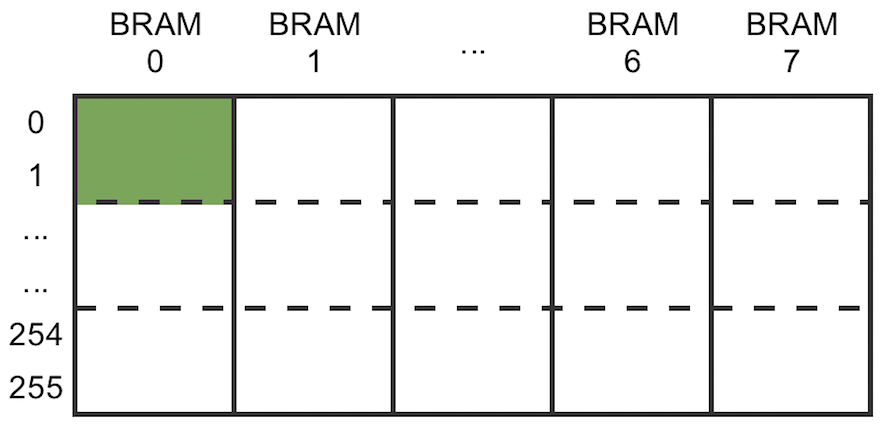
\includegraphics[width=0.40\textwidth]{3-interleave-3a.png}
  \caption{Memory organization of a single double-pumped bank.}
  \label{fig:3-interleave-3}
\end{figure}



\subsection{Element-wise Double-pumping}
\label{sec:wise}
By observing the streaming access pattern more closely with respect to the organization of BRAM primitives, it is clear that when a cache line boundary is crossed, each offset is read once per cycle at most, but never twice at the same offset. By exploiting this observation, a variation of the previous solution is possible which removes the need for two banks per stream buffer. \autoref{fig:3-element-wise-1} shows a single stream buffer where eight horizontal BRAMs contain a cache line. Each BRAM is double pumped as shown in \autoref{fig:3-element-wise-2}. The green box shows that a single element is located within the same BRAM primitive, similarly as in the previous solution.\\
Since two banks are no longer required, all cache lines fit within the same primitive resulting in a utilization of 100\% per BRAM primitive. For eight read ports roughly 52\% of the BRAM primitives are used. Also, there is no longer need for the first level of multiplexing, that reduces the per read port multiplexing to 512:1. Despite these improvements, this solution still requires 70144 LUTs utilize roughly 13\% of the resources.\\
While the design would fit theoretically, each BRAM primitive will have a fan-out equal to the number of read ports. Since getting data out of a BRAM and into processing logic is complex at the target frequency of \SI{200}{\mega\hertz}, the additional fan-out problem does not make this easier. Besides that, using more than half of the available BRAM primitives means that multiple large columns of BRAM primitives are used, scattered all over the FPGA as shown in Section \ref{sec:fpga-arch}. This complicates a unified access latency for each data entry (also keep the fan-out in mind) due to wiring delays across the entire FPGA. Pipelining helps with timing closure, but also increases the read latency of the buffer, a critical metric in the design.

% luts = 512 to 1 mux with 64b data width for 8 read ports. thus 137 * 64 * 8 = 70144 luts total. kut15p = 522720 luts. = 13.4\%\\

%\begin{figure}[H]
%  \centering
%  \begin{subfigure}[c]{.5\textwidth}
%    \centering
%    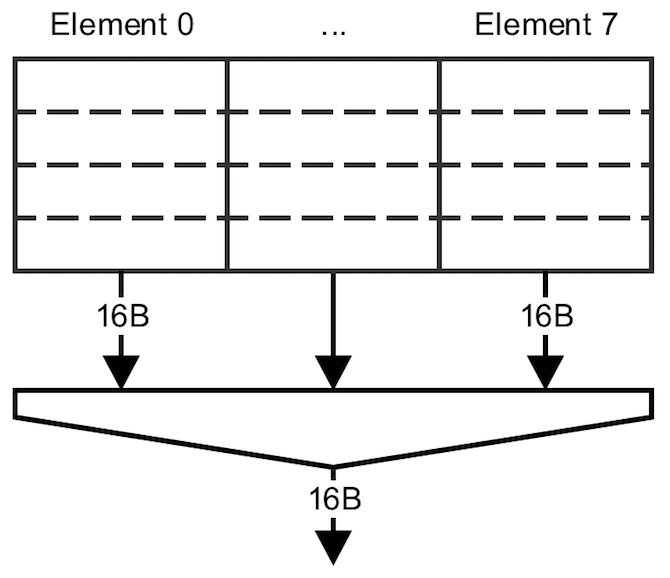
\includegraphics[width=0.6\linewidth]{3-element-wise-1.png}
%    \caption{Element selection from eight BRAM primitives.}
%    \label{fig:3-element-wise-1}
%  \end{subfigure}%
%  \begin{subfigure}[c]{.5\textwidth}
%    \centering
%    \includegraphics[width=0.8\linewidth]{3-element-wise-2.png}
%    \caption{Memory organization of a single stream buffer.}
%    \label{fig:3-element-wise-2}
%  \end{subfigure}
%  \caption{Element-wise double-pumping.}
%  \label{fig:3-element-wise}
%\end{figure}

\begin{figure}[htb!]
\ffigbox[\textwidth]
  {
    \begin{floatrow}
    \ffigbox[\linewidth]
      {\captionof{subfigure}{Element selection from eight BRAM primitives.}
      \label{fig:3-element-wise-1}}
      {\includegraphics[width=0.65\linewidth]{3-element-wise-3.png}}
    \ffigbox[\linewidth]
      {\captionof{subfigure}{Memory organization of a single stream buffer.}
      \label{fig:3-element-wise-2}}
      {\includegraphics[width=0.80\linewidth]{3-element-wise-2.png}}
    \end{floatrow}%
  }
  {\caption{Element-wise double-pumping.}\label{fig:3-element-wise}}
\end{figure}



\subsection{Cache Line Duplication}
\label{sec:duplication}
Duplication guarantees that each read port has access to every element in every cache line at any time. \autoref{fig:3-duplication} shows a possible architecture for cache line duplication. Each read port has a copy of every cache line in each stream buffer, removing the need for large selection logic. The drawback is that the required memory primitives scale linearly with the number of read ports. As shown in Section \ref{sec:naive-design}, the number of supported streams has been decreased to 64 in order to save memory primitives and have resources to spare for control logic and the AFU. A single copy of all buffered cache lines for all streams requires roughly \SI{2}{\mega\byte} or 52\% of BRAM resources. This becomes \SI{16}{\mega\byte} or 416\% for eight read ports which is four times as much as available on the target FPGA. Each read port also has to select the right element. A 512:1 multiplexer is required and if the BRAMs are double-pumped, the total LUT consumption is roughly 13\%. It is obvious that this solution will not fit the target FPGA either. However, the benefit is that the wiring per read port stays within this slice that should make wire routing easier. Also the fan-out per BRAM output has decreased from eight to one, in comparison with the element-wise double-pumping proposal in Section \ref{sec:wise}.

%luts (best case with double pumping for mux reuse) = 137 (table) * 64 (data width) * 8 read ports

\begin{figure}[H]
  \centering
  \includegraphics[width=0.30\textwidth]{3-duplication.png}
  \caption{Stream buffer duplication for each read port.}
  \label{fig:3-duplication}
\end{figure}



%\subsection{Rotating Cache Line Buffer}
%\todo{- add rotating buffer, see memory slides. similar to cell ask Peter how.\\
%- provides a buffer interface to each read port with two consecutive cache lines. When one is fully read, it will be shifted out and the next cache line will be placed in the buffer, therefore limiting the stream buffer to at most one read at cache line granularity per cycle.\\
%- specific to streaming access since you know you can keep part of the data since you will read consecutively.\\
%}

%\begin{figure}[H]
%  \centering
  %\includegraphics[width=0.90\textwidth]{1-model-of-computation.pdf}
%  \caption{.}
%  \label{fig:2-rotating-buffer}
%\end{figure}



\subsection{True Dual Port BRAM}
Finally, memory primitives can be used with multiple ports. A BRAM can be configured as either a simple dual port or a true dual port, as mentioned in Section \ref{sec:fpga-characterization}. In the case of a simple dual port, one port is a designated read port and the other a designated write port. The ports of a true dual port can be configured on-the-fly to act as either a read or write port. Due to the read-write imbalance of writing a cache line in one cycle and completely reading it for eight cycles, the flexibility of a TDP memory seems appealing. However, the effective capacity of a BRAM in TDP mode is reduced to \SI{18}{\kilo\bit}. Therefore, not only are twice the number of primitives required to obtain the same effective capacity, but also complex control logic to configure the ports on-the-fly is required. Even worse is that the previously used configuration of 512 entries is not available in TDP mode. Instead, the smallest number of entries is 1024 with a data width of \SI{36}{\bit}. This means that any of the previously discussed proposals will require twice as much BRAM primitives,not to speak about the additional control logic.
%Besides that, constraining concurrent reading and writing potentially limits throughput in specific cases. 



\subsection{Summary of Naive and Traditional Designs}
Traditional solutions for multi-ported memories have been shown above to not satisfy the desired requirements. Interleaving is an effective way to increase the number of read ports without increasing the required memory primitives. It does, however, pose the problem of under-utilized BRAM primitives and requires large multiplex structures that do not fit in the FPGA resource budget, not to speak of the wiring nightmare that will occur.\\
Element-wise double-pumping is a promising architecture. However, the fan-out of eight for every BRAM and the large columns of BRAM primitives scattered around the FPGA will require additional pipeline registers. This increases a critical metric: the read latency of the AFU.\\
While duplication solves the problem of the large multiplexing structures and the fan-out, there is no resource budget for it. Double-pumping BRAM primitives improves utilization and decreases the required LUTs, but does not solve the underlying problem.\\
The bottom line is that duplication is needed to mitigate the fan-out and, therefore, the wiring problem, but not for all cache lines.

%\todo{- mention rotating buffer; nice but limited to streaming. hurts throughput in more general case such as when changing this into a cache\\
%}



\section{Proposed Architecture}
\label{sec:final-design}
In essence there is a conflict between storing enough cache lines to hide the latency of OpenCAPI, and providing eight individual read ports to the AFU. Simultaneously, on the one hand wiring delay must be taken into account, and on the other hand not all of the available memory resources can be used. Therefore, the proposed multi-stream buffer architecture is split into two levels by exploiting different memory primitives. \autoref{fig:3-solution} shows both levels, \textit{L1} and \textit{L2}, analogous to cache naming conventions.
\begin{itemize}
  \item{\textbf{L1} is a 'small' buffer that is fed by L2. It stores a subset of consecutive cache lines per stream which are duplicated for each read port. This way, each read port has access to exactly the same data and there are no large multiplexer structures required.}
  \item{\textbf{L2} is a ‘big’ buffer that gets up to one new cache line every cycle through OpenCAPI. It is targeted to cover the latency of OpenCAPI by using large memory primitives and therefore does not consume all memory resources as was previously the case.}
\end{itemize}
L1 is optimized for low-latency and multiple read port access while L2 is optimized for memory capacity to cover the latency of OpenCAPI. By choosing the appropriate memory primitive for each level, an architecture can be devised that complies with the requirements and does not consume all available resources while doing so. To keep all duplicate cache lines synchronized in L1, L2 writes new data to all BRAMs simultaneously.

\begin{figure}[H]
  \centering
  \includegraphics[width=0.70\textwidth]{3-solution.pdf}
  \caption{Proposed stream buffer architecture with two levels of buffering.}
  \label{fig:3-solution}
\end{figure}

The proposed architecture mitigates the fan-out problem from the critical AFU read path to a signal path outside of this domain, namely, between the L2 and L1 buffers. This gives us more time to move data out of the URAMs and into all BRAMs simultaneously. However, since cache line granularity data is moved from L2 to L1, the number of fan-out signals increases. Pipeline stages can be added to overcome this if necessary, due to the fact that memories are located in specific columns as shown in Section \ref{sec:fpga-arch}. The smaller BRAM arrays in this proposed architecture, as compared to the element-wise double-pumped architecture, make it easier to obtain unified access latency for each data entry. This is also achieved by supplying a BRAM array per read port such that cache lines used in the near future can be located closest to their consumer.\\
Since L1 is basically a smaller version of the proposed data duplication architecture, the same amount of LUT resources of roughly 13\% is required. Depending on the chosen configuration as to the number of streams and the number of cache lines, resource requirements differ. Section \ref{sec:design-choice} describes the design choices made in more detail.

  \chapter{Design Methodology}
\label{ch:method}
This chapter briefly introduces a cell-based design methodology with an inherent ready-valid protocol. The methodology consists of a workflow and cell-based design library. To motivate the ease-of-use and applicability of the methodology, several complex examples are shown.

%\todo{
%- Read up on counterflow pipeline and see if there is an analogue.\\
%- Andy, do you think that your methodology only works for streaming based accelerators or for all kinds of logic? Did you try it with other types of logic as well?\\
%}





\section{Design Philosophy}
The methodology described is designed over a course of several years by Andrew K. Martin from the IBM Austin Research Lab. The initial ideas concerning this methodology originate from a paper published in 2001 called \textit{The Theory of Latency-Insensitive Design} \cite{delay-insensitive}. It describes the fundamentals of a correct-by-construction design methodology. This paper forms the basis of the ready-valid design methodology by Andrew K. Martin \cite{andy}.



\subsection{The Theory of Latency-Insensitive Design}
The paper \cite{delay-insensitive} presents a foundation of a correct-by-construction methodology which separates a system based on communication and computation. A system is defined as a set of synchronous computational processes that exchange data with one another over communication channels. An abstract protocol is used for communication whose main characteristic is to be insensitive to the latencies of the channels. The protocol works under the assumption that the computational processes are stallable and guarantees that computational processes behave correctly independently of the channel latencies. This enables changing the latency of a communication channel without affecting the functionality of the system, which is a useful property for hardware design.\\
Suppose a system is implemented, but due to wire delay timing constraints are not met. This theory guarantees that a relay station, or register, can be inserted in the communication channel without affecting the functionality. Therefore no costly redesigns are needed.\\
The idea of relay stations is borrowed from the pipelining concept and a relay station in function is similar to a register. This approach relaxes timing constraints during the early design phases when accurate measures of delay paths between computational processes are not yet available. If after physical implementation a mismatch exists between the timing constraint and the communication channel delays, they can easily be corrected by inserting the correct amount of relay stations. Since every computational process operates according to the latency-insensitive protocol, no changes are required in order to reflect the necessary changes in the communication channel latencies.



\subsection{Ready-Valid Design Methodology}
Typically, there are three types of flow control concepts a hardware designer can choose from.
\begin{itemize}
  \item{\textbf{Credit-Based} protocol manages credits between a start and end module. If no more credits are available, the logic in between is stalled.}
  \item{\textbf{Cycle-Based} protocol indicates after how many cycles a response will be received for sent data for example. A downside is that it is difficult to decide on what to do when no response is received, or more generally, what to do when the protocol breaks.}
  \item{\textbf{Ready-Valid-Based} protocol has a valid signal to indicate the validity of an output and a ready signal to indicate it is ready to receive a new input. Usually it is only used between large modules in a system.}
\end{itemize}

The ready-valid design methodology discussed here differs from the typical ready-valid protocol since it uses the paradigm all the way down to the lowest level of a system. This combined with the latency-insensitive design theory results in a methodology that consists of a library of cells that are analogous to the computational processes. These cells are interconnected using a ready-valid protocol, the communication channel, which makes it possible to stall at a cell granularity. This means that progress is made whenever possible.\\
The cell-based nature allows to easily understand a design by following the ready-valid protocol and associated data, if present. Due to a rich library of cells, writing a design mostly consists of connecting the cells and compiling the design. Since cells are correct-by-construction, errors only consist of typos, signal width mismatches, and other easily fixable errors. After that the ready-valid protocol is functionally correct. Only the associated data signals could not be functionally correct. This means that transformations on the data signal have been done incorrectly.



\subsection{Ready-Valid Communication Protocol}
In general, a cell within the ready-valid design methodology has a set of configuration parameters and a set of input and output signals, as shown in \autoref{fig:7-cell}. Examples of configuration parameters are the number of inputs or the signal width in bits of each data input. The input and output signals are named according to a predetermined scheme. The signals on the left of the generic cell are all called input signals, even though physically the ready signal is an output. Together they form the input interface and follow the naming convention of \texttt{i\_v} and \texttt{i\_r} for the valid and ready signal, respectively. The data signal, typically denoted by \texttt{i\_d}, is not obligatory and some cells only have ready and valid signals. According to the same naming convention, the output signals are called \texttt{o\_v}, \texttt{o\_d} and \texttt{o\_r} and together form the output interface.

\begin{figure}[H]
  \centering
  \includegraphics[width=0.50\textwidth]{7-cell.pdf}
  \caption{Input and output signals of a generic cell.}
  \label{fig:7-cell}
\end{figure}

The ready-valid protocol used by the cells on the communication channels between computational processes is a handshaking protocol. Progress is only made if both the input valid and ready signal are asserted for a cell in a given clock cycle. The communication channel is explicit and building a system mostly consists of connecting cells by a communication channel consisting of a ready and valid signal. In a system consisting of multiple cells, the naming convention dictates that a preceding cell is called \textit{upstream} and the successive cell is called \textit{downstream}.\\
In the ready-valid design methodology, a cell or computational processes can be combinatorial or sequential logic. Examples of each type will be shown in Section \ref{sec:cell-lib}. Independently of the type, a cell has at least two ready-valid signal pairs. One as input and one as output interface. In terms of physical input and output signals, a cell has two inputs, \texttt{i\_v} and \texttt{o\_r}, and two outputs, \texttt{i\_r} and \texttt{o\_v}.\\
Typically, when a cell comes out of a reset state, its input ready signal is asserted independently of any downstream cell ready signals it may receive at its output interface. The reason is that progress can be made by supplying the cell with a valid input to be serviced. The output valid signal is asserted when a valid input occurs and the cell is ready to service this valid input. In other words, the cell is not in a stalled state. If the cell is in a stalled state, the input ready signal will be de-asserted to indicate the upstream cells that a stall occurred. The concept of indicating to upstream cells that a cell is stalled is called \textit{applying back-pressure} in the ready-valid design methodology. An example of applying back-pressure could be that a cell requires data from multiple locations that do not arrive at the same time. Therefore, the cell has to be stalled until all data is available and back-pressure has to be applied to upstream cells. It is important to note that the input ready signal is only de-asserted if the cell is stalled, or if a downstream cell has stalled that induces a chain reaction of stalls. This is different from a typical ready-valid protocol where the ready signal is de-asserted after a transaction occurred (an example is AXI \cite{amba4}).



\subsection{Differences Compared to Asynchronous Design}
At first sight, the ready-valid design methodology may be interpreted as an asynchronous design methodology. However, there are several differences between the two. First of all, asynchronous design does not use a clock, while this methodology does. That means that the presentation of a ready or valid signal would be by changing the value of a signal, rather than by asserting it.\\
The ready-valid design methodology allows a ready or valid signal to be asserted in one cycle, and then de-assert in a subsequent cycle, even if the complimentary signal (valid or ready, respectively) was never asserted and no transaction took place. Similarly, the data corresponding with a valid signal is allowed to change on subsequent cycles, even though no corresponding ready signal was received and hence no data transfer took place. This would not work in an asynchronous framework and may have implications on design.\\
Finally, the \texttt{base\_aburp} and \texttt{base\_alatch} cells (discussed in Section \ref{sec:burp}) loose their meaning in an asynchronous framework. Although something analogous may be needed to maintain reasonable timing constraints between valid and data signals. 





\section{Workflow}
\label{sec:workflow}
Besides a supplied cell library, the ready-valid design methodology also comes with a workflow of several steps and special cells to speed up the workflow.
\begin{enumerate}
  \item{\textbf{Build the System} The first step is build the system with the provided cells, possibly accompanied by other logic. Relay stations should be placed between combinatorial cells and with experience proper locations are easily identified. These relay stations are analogous to configurable registers.}
  \item{\textbf{Functional Verification} After compiling the design from Step 1 and fixing compiler errors and warnings, the ready and valid signals should be verified first. Make sure they are always defined and only then verify the associated data signals. If more in-depth debugging is required, trace the valid and ready signals throughout the system and make sure cells apply back-pressure when needed, in order to not lose valid information.}
  \item{\textbf{Synthesis and Timing Constraints} After functional verification, the system should be synthesised to see if it meets the timing constraints. If the constraints are met, the next step can be started. If the constraints are not met, the register cells instantiated in Step 1 should simply be reconfigured accordingly or inserted multiple times to allow for multi-cycle communication channels; this step should be restarted. This process continues until the timing constraints are met everywhere in the design.}
  \item{\textbf{Physical Verification} After meeting the timing constraints, the system has to be verified again. When this step finishes successfully, it is possible to go back to Step 3 and tweak the design in order to improve metrics such as area or operating frequency.}
\end{enumerate}



\subsection{Tweaking Relay Stations}
The positioning of registers or relay stations depends on whether the system will be implemented on an ASIC or FPGA. For an FPGA, distribution of the wires is more difficult than driving them. FPGAs have buffers and repeaters everywhere to simplify this for the designer.\\
An ASIC does not have this luxury, thus the instinct of the designer concerning relay station positioning should be different. For ASICs, driving strength is more difficult. Positioning relay stations should take the combinatorial path of the function that is being implemented into account.



\subsection{Synthesis Helper Cells}
Systems or modules within a system typically have a large number of input and output signals, especially when data widths are large. When implementing a design on an FPGA, the provided tools try to connect each input or output signal of the system or module to a physical pin on the FPGA package. Depending on the size of the system or module and target device, there might not be enough physical pins for the tool to finish implementation. However, obtaining an estimate on metrics such as area and operating frequency is often desired, also for modules within the system.\\
In order to speedup synthesis and overcome the described problem, two helper cells are present in the cell library called \texttt{base\_input\_lat} and \texttt{base\_output\_lat}. These modules are parametrised shift registers. The \texttt{base\_input\_lat} cell is to be attached to one physical pin on the FPGA package and to all input signals of the system or module to be synthesised. Similarly but in opposite direction, the \texttt{base\_output\_lat} cell is used to connect multiple output signals to a single physical pin.





\section{Delay-Insensitive Cell Library}
\label{sec:cell-lib}
The cell library that is part of the ready-valid design methodology has been published on GitHub \cite{andy-lib} and is a work in progress. At the moment of writing, the version published on November 16, 2017 is used throughout this document.



\subsection{Diagram Legend and Naming Conventions}
Throughout this thesis, implementation diagrams and signal names follow a predefined scheme consisting of object shapes and colors and naming conventions to indicate various characteristics.



\subsubsection{Diagram Legend}
\label{sec:legend}
A cell is a submodule that is part of the design library. \autoref{fig:6-library-1} shows a combinatorial cell and \autoref{fig:6-library-2} a sequential cell. \autoref{fig:6-library-3} shows a (de)multiplexer cell, depending on the direction of the input and output signals.\\
Besides cells from the library, also logic that is not a cell can be included in a design called a submodule, shown in \autoref{fig:6-library-4}. \autoref{fig:6-library-5} shows a combinatorial arithmetic operation. A typical example is an addition to increment a counter. That could be implemented using a sequential cell. A common construct in this methodology is shown in \autoref{fig:6-library-6} and is called an act signal, often denoted by \texttt{*\_act}. It is a logical AND operation on a valid and ready signal, for example used as an enable signal.\\
To allow for hierarchy in diagrams, a collection of multiple cells and submodules can be replaced by a module. The module name always starts with a capital and is shown in \autoref{fig:6-library-7}. To show multiple identical instantiations of a cell or module, a generate construct is indicated by a green box. Multiple objects stacked behind each other and the number of instantiations is shown in the lower right corner, as shown in \autoref{fig:6-library-8}. The input and output signals are solid lines for the first instantiated object and dashed for any other objects stacked behind it.\\
Typically, only the downstream signals are shown in the diagrams and only rarely are upstream signals shown, such as ready signals. An act construct typically shows the ready signal until it is terminated.

\begin{figure}[h]
  \begin{subfigure}{.33\textwidth}
    \centering
    \includegraphics[width=0.60\linewidth]{6-library-1.pdf}
    \caption{Combinatorial cell.}
    \label{fig:6-library-1}
  \end{subfigure}%
  \begin{subfigure}{.33\textwidth}
    \centering
    \includegraphics[width=0.25\linewidth]{6-library-2.pdf}
    \caption{Sequential cell.}
    \label{fig:6-library-2}
  \end{subfigure}%
  \begin{subfigure}{.33\textwidth}
    \centering
    \includegraphics[width=0.15\linewidth]{6-library-3.pdf}
    \caption{(De)multiplexer cell.}
    \label{fig:6-library-3}
  \end{subfigure}\\[1ex]
  \begin{subfigure}{.33\textwidth}
    \centering
    \includegraphics[width=0.60\linewidth]{6-library-4.pdf}
    \caption{Combinatorial submodule.}
    \label{fig:6-library-4}
  \end{subfigure}%
  \begin{subfigure}{.33\textwidth}
    \centering
    \includegraphics[width=0.25\linewidth]{6-library-5.pdf}
    \caption{Combinatorial arithmetic.}
    \label{fig:6-library-5}
  \end{subfigure}%
  \begin{subfigure}{.33\textwidth}
    \centering
    \includegraphics[width=0.80\linewidth]{6-library-6.pdf}
    \caption{Act signal.}
    \label{fig:6-library-6}
  \end{subfigure}\\[1ex]
  \begin{subfigure}{.5\textwidth}
    \centering
    \includegraphics[width=0.40\linewidth]{6-library-7.pdf}
    \caption{Clocked module.}
    \label{fig:6-library-7}
  \end{subfigure}%
  \begin{subfigure}{0.5\textwidth}
    \centering
    \includegraphics[width=0.80\linewidth]{6-library-8.pdf}
    \caption{Generate construct.}
    \label{fig:6-library-8}
  \end{subfigure}
  \caption{Implementation diagram conventions.}
  \label{fig:6-library}
\end{figure}

%\todo{
%- Fix vertical alignment.\\
%- Fix combinatorial arithmetic cutoff.\\
%}



\subsubsection{Naming Conventions}
Typically the input and output signals of any cell or module start with \texttt{i\_*} and \texttt{o\_*}, respectively. Internal signals of a cell or module also follow a naming convention, depending on the location of the signal with respect to the sequential elements and whether the signal has a special purpose, such as valid, ready, data, or act. Often the cell or module the valid signal originates from is included in the signal name. An example could be the output valid signal of the initial register cell: \texttt{s1\_reg\_v}. Another example could be a data signal after a counter cell operating after four pipeline stages from the input signals: \texttt{s4\_cntr\_d}. Listings shown later on provide more naming convention examples.\\
Cell or module instantiations follow a similar naming convention, indicating the pipeline stage the signal operates in, the cell or module name and indication if it is a combinatorial or sequential element. Typically combinatorial elements have no suffix while sequential elements have a \texttt{*\_reg} or \texttt{*\_lat} suffix, standing for register and latch, respectively. In the design methodology, a register is a sequential cell with a ready-valid pair as input and output. A latch is a sequential cell without ready-valid pairs.\\
Most cells have a prefix, either \texttt{a*} or \texttt{e*}. For historic reasons, the \texttt{a*} stands for \textit{asynchronous} and is used to mean that the cell has a ready-valid interface. The \texttt{e*} prefix means \textit{encoded} and typically refers to the select signal. Cells without this prefix typically have a decoded select signal.\\
Most of the cells are implemented as big-endian, but for certain cells the endianness matters. For example for multiplexers. For those cells a little-endian variant exists and is denoted by the suffix \texttt{*\_le}.





\subsection{Pass Gate Cell}
%\todo{
%- listing: fix white lines in dark background.\\
%- listing: center code \url{http://www.mrunix.de/forums/showthread.php?43153-lstinputlisting-zentriert}\\
%- listing: highlight Verilog function clog2 for example.\\
%- listing: highlight module instantiation.\\
%- listing: highlight bit signals "1'b1"\\
%}

A basic cell is the pass gate \texttt{agate} shown in \autoref{lst:gate}. Due to its straightforward behavior, it acts as an initial example of a cell from the library. The function of the cell is to grant access to a downstream ready-valid cell if a certain condition is met. The condition is supplied to the cell as the one bit input enable signal \texttt{en}. The cell has two additional input signals that are the input valid signal \texttt{i\_v} and output ready signal \texttt{o\_r}. As the listing shows, the two output signals \texttt{i\_r} and \texttt{o\_v} are nothing more than a logical AND operation on one of the input signals and the input enable signal. The \texttt{width} parameter is used to configure the number of ready-valid pairs this cell handles.\\
An application example of the pass gate cell is to grant read access to a memory, but only if the memory contains valid data. In this example, the input valid signal could indicate a valid read request, accompanied by a memory address as data signal. The enable signal could originate from a counter cell that keeps track of the number of valid data entries.

\begin{lstlisting}[style={verilog-style}, caption=Pass gate cell from the ready-valid cell library., label=lst:gate]
module base_agate #
(
  parameter width = 1
)
(
  input  [width-1:0] i_v,
  output [width-1:0] i_r,
  input  [width-1:0] en,
  output [width-1:0] o_v,
  input  [width-1:0] o_r
);

  assign i_r = en & o_r;
  assign o_v = en & i_v;
endmodule
\end{lstlisting}



\subsection{Decode Cell}
\label{sec:decode}
The library also consists of non-ready-valid capable cells such as the decode cell \texttt{decode} shown in \autoref{lst:decode}. The function of this cell is to decode the input signal \texttt{din} if a certain condition is met. Similar to the \texttt{agate} cell, the input enable signal is called \texttt{en}. Due to the parametrized nature of the cell library, each cell has a variable width. In this case the input data width is configured using the \texttt{enc\_width} parameter that implies the output width as well. In order to support the parametrization, a Verilog generate statement is used in combination with a for-loop. During compilation, the for-loop is unrolled followed by generation of the associated hardware.

\begin{lstlisting}[style={verilog-style}, caption=Decode cell from the ready-valid cell library., label=lst:decode]
module base_decode #
(
  parameter enc_width = 1,
  parameter dec_width = 2 ** enc_width
)
(
  input                  en,
  input  [enc_width-1:0] din,
  output [dec_width-1:0] dout
);

  genvar i;
  generate
    for(i=0; i<dec_width; i=i+1) begin : Gen
      assign dout[i] = en & (din == i);
    end
  endgenerate
endmodule
\end{lstlisting}



\subsection{Multiplexer Cell}
\label{sec:mux}
Another basic non-ready-valid capable cell is the multiplexer cell \texttt{emux} shown in \autoref{lst:mux}. In line with the cell library philosophy, a \texttt{width} parameter is available. Another recurring configuration parameter in the ready-valid cell library is the \texttt{ways} parameter. This parameter typically indicates the number of inputs of a cell, which in this case is the number of inputs to select from. This parameter implies the encoded signal width of the input select signal \texttt{sel} that uses the built-in \texttt{\$clog2()} function of Verilog. This function returns the logarithm in base two of the input argument to the function.

\begin{lstlisting}[style={verilog-style}, caption=Multiplexer cell from the ready-valid cell library., label=lst:mux]
module base_emux #
(
  parameter width = 1,
  parameter ways = 2,
  parameter sel_width = $clog2(ways)
)
(
  input  [(width*ways)-1:0] din,
  input  [sel_width-1:0]    sel,
  output [width-1:0]        dout
);

  wire [width-1:0] din_array [ways-1:0];

  genvar i;
  generate
    for(i=0; i<ways; i=i+1) begin : Gen
      assign din_array[i] = din[(i+1)*width-1:i*width];
    end
  endgenerate

  assign dout = din_array[sel];

endmodule
\end{lstlisting}



\subsection{Ready-Valid Merge Cell}
The reason for showing the previous two cells, besides introducing typical signal and parameter names, is to illustrate how a ready-valid cell can be constructed from non-ready-valid capable cells. A ready-valid merge cell, shown in \autoref{lst:merge}, merges \texttt{ways} inputs, each with \texttt{width} wide data. The input select signal \texttt{sel} is first decoded using the decode cell discussed in Section \ref{sec:decode}, with the enable signal always asserted. The output valid signal is determined by whether the particular input is valid and which input was selected. Since both signals are \texttt{ways} bits wide, a logical reduction OR operator is used. Similarly, but opposite, the input ready signal is determined by which input is selected, since that input is ready to receive a new valid input data, and the output ready signal to determine if the downstream module is ready. Since there are \texttt{ways} input signals and the output ready signal is only one bit, it is replicated as often as there are inputs. Finally the input data \texttt{i\_d} is selected using the multiplexer shown in Section \ref{sec:mux}.

\begin{lstlisting}[style={verilog-style}, caption=Ready-valid merge cell from the ready-valid cell library., label=lst:merge]
module base_aemux #
(
  parameter ways = 2,
  parameter width = 1,
  parameter sel_width = $clog2(ways)
)
(
  input  [ways-1:0]         i_v,
  output [ways-1:0]         i_r,
  input  [(width*ways)-1:0] i_d,
  input  [sel_width-1:0]    sel,
  output                    o_v,
  input                     o_r,
  output [width-1:0]        o_d
);

  wire [ways-1:0] sel_dec;
  base_decode_le#(.enc_width(sel_width),.dec_width(ways))
    isel_dec(.din(sel),.dout(sel_dec),.en(1'b1));

  assign o_v = |(sel_dec & i_v);
  assign i_r = sel_dec & {ways{o_r}};

  base_emux_le#(.ways(ways),.width(width))
    imux(.sel(sel),.din(i_d),.dout(o_d));

endmodule
\end{lstlisting}





\section{Advanced Examples}
The previous section introduced the cell library that is part of the ready-valid methodology. This section uses the presented conventions to introduce several advanced examples of the methodology.



\subsection{Interfacing with a Credit-Based Interface}
A common interface type is based on credits, which is for example used by interconnects such as PCI Express and OpenCAPI to control the flow of packets. Typically it is used to share a resource and give each consumer a credit if a credit is available. When no more credits are available, consumers are no longer granted access until a credit becomes available again. The interaction with modules that are not based on the ready-valid protocol such as memory primitives may serve as an example. Memory primitives typically consist of a read and write interface of three signals: enable, address, and data. More details concerning memory primitive interaction will be discussed in Section \ref{sec:rvmem}. Another use case is when the ready-valid cells and modules consume too much area in the design. A local transition to a credit interface (and back) possibly overcomes this problem.\\
The cell library provides two cells to transition from a ready-valid protocol to a credit-based protocol (source) and vice versa (sink). The cells are named \texttt{credit\_src} and \texttt{credit\_snk}, respectively. \autoref{fig:7-credit} shows a generalized setup and interaction with ready-valid-based cells.

\begin{figure}[h]
  \centering
  \includegraphics[width=0.70\textwidth]{7-credit.pdf}
  \caption{Diagram of a generalized transition between a credit- and ready-valid-based protocol.}
  \label{fig:7-credit}
\end{figure}



\subsection{Synchronization of Multiple Control Flows}
When designs get more complex, often multiple control flows have to be synchronized with each other before progress can be made. The cell library provides a single cell to synchronize \textit{N-to-M} inputs and outputs named \texttt{combine}. Two examples are shown below of uses of this cell during the implementation of the multi-stream buffer.



\subsubsection{Many-to-One}
\label{sec:sync-1}
The first encounter involves synchronization of multiple inputs with one output, as shown in \autoref{fig:7-sync-1}. In this example, the downstream module \textit{Request Consumer} is shared by two ready-valid-based modules, shown on the left of the \textit{Combine} cell. The \textit{Request Producer} produces a request consisting of a ready-valid pair and a stream identifier as associated data signal. Since a resource is shared downstream, that is only able to accept a predefined number of outstanding requests, each request from the producer has to obtain a unique tag.\\
There are various scenarios possible in this case. If the downstream module is not ready, both the \textit{Request Producer} and the \textit{Resource Manager} have to stall in order to prevent discarding a valid request or waste a precious tag, or both. Similarly, if the \textit{Request Producer} has no valid request, the \textit{Resource Manager} should not waste a tag and, vice versa, the \textit{Request Producer} should not discard a valid request when all tags are in use. The bottom line is that these two control flows have to synchronized.

\begin{figure}[H]
  \centering
  \includegraphics[width=0.70\textwidth]{7-sync-1.pdf}
  \caption{Diagram of a many-to-one synchronization example.}
  \label{fig:7-sync-1}
\end{figure}

To do so, the cell library provides a cell that can be configured to accommodate any number of inputs and outputs, independently of each other. \autoref{lst:sync-1} shows the ease of use of the \texttt{combine} cell (line 26), by simply connecting the various cells and modules together and configuring the number of inputs and outputs to synchronize. In this example, a hypothetical \textit{Request Producer} module is used and a simplified \textit{Resource Manager} cell from the library. The \texttt{res\_mgr} cell provides a configurable number of unique tags that can be used to associate with a request. The tag return interface has been omitted for simplicity.

\begin{lstlisting}[style={verilog-style}, caption=Many-to-One synchronization example., label=lst:sync-1]
  wire s1_req_v, s1_req_r;
  wire [nstrms_width-1:0] s1_req_sid;
  request_producer # (
    .width  (nstrms_width)
    ) is0_req_prod (
    .clk    (clk),
    .reset  (reset),
    .o_v    (s1_req_v),
    .o_r    (s1_req_r),
    .o_d    (s1_req_sid)
  );

  wire s1_mgr_v, s1_mgr_r;
  wire [tag_width-1:0] s1_mgr_tag;
  base_res_mgr # (
    .width  (tag_width)
    ) is1_res_mgr (
    .clk    (clk),
    .reset  (reset),
    .o_v    (s1_mgr_v),
    .o_r    (s1_mgr_r),
    .o_d    (s1_mgr_tag)
  );

  wire s1_comb_v, s1_comb_r;
  base_acombine # (
    .ni     (2),
    .no     (1)
    ) is1_cmb (
    .i_v    ({s1_req_v, s1_mgr_v}),
    .i_r    ({s1_req_r, s1_mgr_r}),
    .o_v    (s1_comb_v),
    .o_r    (s1_comb_r)
  );

  request_consumer # (
    .width  (nstrms_width),
    .tag    (tag_width)
    ) is2_req_cons (
    .clk    (clk),
    .reset  (reset),
    .i_v    (s1_comb_v),
    .i_r    (s1_comb_r),
    .i_sid  (s1_req_sid),
    .i_tag  (s1_mgr_tag)
  );
\end{lstlisting}



\subsubsection{One-to-Many}
Another encounter involves synchronization of a single input with multiple outputs, as shown in \autoref{fig:7-sync-2}. In this example, an incoming read request from the AFU starts two separate processes. The first process calculates an address to index a memory based on a global pointer stored in one of the \textit{Stream Pointer} modules and the number of other read ports accessing the same stream. The second process updates the global pointer based on all streams requested and will request new data upstream if needed. More details concerning the operation of the modules used can be found in Section \ref{sec:l1-ptr} and \ref{sec:rd-port}.\\
Similarly to the many-to-one synchronization example shown above, the \texttt{combine} cell is configured with the appropriate number of inputs and outputs and connects the incoming read request to both process modules. In essence, it would be similar to \autoref{lst:sync-1}, traversed in reverse order. While the two presented examples have either one input or output, the \texttt{combine} cell is able to synchronize any number of inputs with any number of outputs.

\begin{figure}[H]
  \centering
  \includegraphics[width=0.90\textwidth]{7-sync-2.pdf}
  \caption{Diagram of a one-to-many synchronization example.}
  \label{fig:7-sync-2}
\end{figure}



\subsection{Timing Closure Using Relay Stations}
\label{sec:burp}
%\todo{
%- areg cell mostly used as reg and to fix timing. Other use cases for the base\_reg is when you have feedback in your path. You need a storage element otherwise it will be a combinatorial loop. A second use case is when you have converging paths to use this. Otherwise a deadlock will arise. These are advanced topics. If Andy would write a book it would be in advanced performance considerations.\\
%- Interesting topic is to prove if latch-burb is functionally equal to burb-latch. This can be set with the lbl parameter in the base\_reg module.
%}

The function of a relay station, as defined in the theory of latency-insensitive design \cite{delay-insensitive}, is fulfilled by the \texttt{reg} cell in the ready-valid design methodology. Typically the \texttt{reg} cell is used as a register for a ready-valid signal pair and the associated data signal. However, due to its parametrized nature, the cell can be easily reconfigured to meet timing by inserting an empty cycle, or to improve resource utilization by removing a cycle, either from the ready or valid path or both.\\
\autoref{lst:7-reg} shows the instantiation of the cell. It contains the typical ready-valid input and output signal pairs and a parameter \texttt{width} to configure the width of the data signal. Unique to this cell is the \texttt{lbl} parameter that stands for latch-burp-latch. When each bit is asserted, the respective cell (\texttt{latch} or \texttt{burp}) is generated.

\begin{lstlisting}[style={verilog-style}, caption=Ready-valid register cell from the ready-valid cell library., label=lst:7-reg]
base_areg # (
  .lbl    (3'b110),
  .width  (width)
) is0_reg (
  .clk    (clk),
  .reset  (reset),
  .i_v    (i_v),
  .i_r    (i_r),
  .i_d    (i_d),
  .o_v    (o_v),
  .o_r    (o_r),
  .o_d    (o_d)
);
\end{lstlisting}



\subsubsection{Latch Cell}
\autoref{lst:7-latch} shows the \texttt{latch} cell from the ready-valid cell library. This cell is used within the \texttt{reg} cell and provides a sequential element in the valid signal path. The \texttt{o\_v} signal is the output of a \texttt{vlat} cell of which the input signal is asserted only when the \texttt{latch} cell receives a valid input or when the downstream cell does not accept the current transfer. Similarly, when an associated data signal is present, an additional \texttt{vlat\_en} cell is generated and is only enabled if the downstream cell accepted the current transfer. This enable signal is also used to drive the \texttt{i\_r} signal.

\begin{lstlisting}[style={verilog-style}, caption=Latch cell from the ready-valid cell library., label=lst:7-latch]
module base_alatch #
(
  parameter width = 1
)
(
  input 	         clk,
  input 	         reset,
  input 	         i_v,
  input  [0:width-1] i_d,
  output 	         i_r,
  output 	         o_v,
  output [0:width-1] o_d,
  input 	         o_r
);

  wire o_v_in = i_v | (o_v & ~o_r);
  wire enable = o_r | ~o_v;
  assign i_r = o_r | ~o_v;
  base_vlat#(.width(1)) ivlat (.clk(clk), .reset(reset), .din(o_v_in), .q(o_v));

  wire [0:width-1] din = i_d[0:width-1];
  generate
    if (width > 0)
      base_vlat_en#(.width(width)) idlat (.clk(clk), .reset(1'b0), 
        .enable(enable), .din(i_d), .q(o_d));
  endgenerate

endmodule
\end{lstlisting}



\subsubsection{Burp Cell}
\autoref{lst:7-burp} shows the \texttt{burp} cell from the ready-valid cell library. This cell is used within the \texttt{reg} cell and provides a sequential element in the ready signal path. The \texttt{o\_v} signal propagates without any latency from the \texttt{i\_v} signal, unless the previous transfer was not completed, indicated by the \texttt{burp\_v} signal. Note that when \texttt{burp\_v} is asserted, the input data signal is not captured in the \texttt{vlat\_en} cell and the previously captured data signal is presented at the output. If not, the current input data is captured and presented and the output. The input ready signal is then equal to the inverse of the \texttt{burp\_v} signal.

\begin{lstlisting}[style={verilog-style}, caption=Burp cell from the ready-valid cell library., label=lst:7-burp]
module base_aburp #
(
  parameter width = 1
)
(
  input 	         clk,
  input 	         reset,
  input 	         i_v,
  input  [0:width-1] i_d,
  output 	         i_r,
  output 	         o_v,
  output [0:width-1] o_d,
  input 	         o_r
);

  wire burp_v;
  wire burp_v_in = ~o_r & (burp_v | i_v);
  assign i_r = ~burp_v;
  assign o_v = i_v | burp_v;
  base_vlat#(.width(1)) ivlat (.clk(clk), .reset(reset), .din(burp_v_in), .q(burp_v));
  
  generate
    if (width > 0) begin
      wire [0:width-1] burp_d;
      assign o_d = burp_v ? burp_d : i_d;
      base_vlat_en#(.width(width)) idlat (.clk(clk), .reset(1'b0), 
        .enable(~burp_v), .din(i_d), .q(burp_d));
    end
  endgenerate
endmodule
\end{lstlisting}





\subsubsection{Register Cell}
\autoref{fig:7-base-areg} shows a simplified view of the \texttt{reg} cell. Internally, the \texttt{burp} and \texttt{latch} cells, discussed in the previous paragraphs, are used. The orange ovals represent combinatorial logic, as shown in \autoref{lst:7-latch} and \autoref{lst:7-burp}.

\begin{figure}[H]
  \centering
  %\includegraphics[width=0.75\textwidth]{7-base-areg.png}
  \includegraphics[width=0.75\textwidth]{6-reg.pdf}
  \caption[Diagram of the relay station cell with lbl - 3'b111.]{Diagram of the relay station cell with \texttt{lbl = 3'b111}.}
  \label{fig:7-base-areg}
\end{figure}

A typical starting point is to configure the cell as \texttt{3'b110} that generates one latch and one burp. This configuration is shown in \autoref{fig:7-base-areg-110} and results in a register in both the ready and valid paths. As mentioned in Section \ref{sec:workflow}, it is good practice to insert a \texttt{reg} cell regularly during the implementation to minimize rewriting of the system description at a later stage. By simply reconfiguring the relay station after the design failed timing, for example, a new compilation can be run immediately without rewriting any code.

\begin{figure}[H]
  \centering
  \includegraphics[width=0.50\textwidth]{6-reg-110.pdf}
  \caption[Diagram of the relay station cell with lbl = 3'b110.]{Diagram of the relay station cell with \texttt{lbl = 3'b110}.}
  \label{fig:7-base-areg-110}
\end{figure}

  \chapter{Implementation}
Section \ref{sec:final-design} made clear that duplication is needed in order to unify access latency for each data entry. Due to exploiting different memory primitives, the proposed architecture consumes less valuable memory resources compared to traditional architectures. By providing an element-sized access granularity and select elements within or close to the memory primitive, the selecting structures are also significantly smaller compared to traditional architectures.\\
%However, not all cache lines have to be duplicated at all times, only the ones that will be read within the foreseeable future. Section \ref{sec:final-design} introduced a high level proposal of a multi-stream buffer architecture using two levels of buffering to solve all of the drawbacks of traditional multi-read-port memory designs.\\
This chapter describes the operation of the proposed design, followed by a section which discusses the design choices made based on resource limitations imposed by the target FPGA. Afterwards the implementation of the proposed architecture is explained in more detail by going through the entire design module by module.

%\todo{- FROM DESIGN DOC: Steps in designing and implementing the APL:
%-- Step 1: split the design in data and control flow parts. First build the core data flow part of the design to see if that will map to the FPGA in the first place (if it can wire it up). The core data flow parts are the BRAM and URAM arrays, so forget about tags etc. Access the arrays with an index and think about it as a direct mapped address.\\

%Interesting note about role of data path and control and how they work together (source: %\url{https://books.google.com/books?id=2-TlBwAAQBAJ&pg=PA122&lpg=PA122&dq=digital+design+data+flow+control+flow&source=bl&ots=CTR8aHB0M5&sig=shzbSfOOnEVJDFkbf11o0rewWRw&hl=en&sa=X&ved=0ahUKEwj2m6GPvc3UAhUEQyYKHRKlCOE4FBDoAQgpMAE#v=onepage&q=digital%20design%20data%20flow%20control%20flow&f=false}):\\
%"To complete the high level synthesis process, a control unit has to be synthesized that implements the schedule. This control unit generates the signals that drive the functional units, interconnect (mux, demux) and registers in the data path - the sequence of execution is as per the generated schedule.\\

%Although there are several styles of controller architectures to choose from [two refs], by far finite state machines are the most popular for digital design. This is also the controller architecture we have chosen in our methodology. We now describe the construction of the fsm from the scheduled htg followed by the subsequent generation of rtl vhdl. The output vhdl code ...\\

%We decided to split the implementation in data and control flow, since the data flow in this case is so much larger (all those BRAMs, URAMs and wiring between them (4k wires = 4x 128B)). First see if that fits and how it is routed.\\

%-- Step 2: dive deeper into the addresses and how they should work. Sounds like using a tag array. Rationale for splitting this from core data flow is that if you are going to access your tag array, after that you are still going to get an index into one of these BRAM arrays. So it does not change the BRAM array piece of the story.\\
%-- Step 3: get into controlling the data flow. The link in Step 1 (Section 8.3 of the book) seems to have interesting information regarding how to slice control, or the FSM. With various sources as well to back it up. Good for thesis.
%}





\section{Functional Operation}
\label{sec:funcop}
Each of the two levels of buffering have different requirements regarding the respective memory primitive. L1 should be optimized for low latency and have enough capacity to cover the latency of L2, while L2 should be optimized for memory capacity to cover the latency of host memory accesses over OpenCAPI. Taking the memory resources presented in Section \ref{sec:fpga-characterization} into account, BRAMs are best suited for L1 since several mega bytes are available and due to their low read and write latency. URAMs are a good fit for L2 since also several mega bytes are available, but each primitive is larger, and requires a slightly higher access latency.



\subsection{AFU Read Request Operation}
\autoref{fig:7-apl-top} shows a block diagram of the interaction between the AFU, the two levels of buffering and a host interface. In theory the host interface could be any current or future interconnect standard, but this particular architecture focusses on the bandwidth specification and cache line size of OpenCAPI 3.0 operating on a POWER architecture host system.\\
Because of the read-only nature of this buffer, there is a clear distinction between the control and data path, or request and response path in this case, which flow in opposite direction. The control flow starts at the AFU, which is able to request eight elements per cycle, each from any stream. An AFU request consists of a ready-valid signal pair and a stream identifier. Each \textit{Read Port} module has its own logic to distribute the requests among the different \textit{L1 Control} modules. Every stream has a separate controller in order to keep track of the current read and write pointers. This holds for both the \textit{L1} and \textit{L2 Control}. If the last element of a cache line in L1 is read, a request is sent to the respective L2 controller which will read a new cache line from the URAM and write it in L1. This frees up an entry in the URAM and triggers L2 to generate a new cache line request for the host. The \textit{Request Generation} module translates a stream number into an address for the host and attaches a unique tag to each request, which also consists of a ready-valid signal pair. Meanwhile, both the L1 and L2 stream controllers calculate addresses to index the \textit{BRAM} or \textit{URAM} module respectively.

\begin{figure}[H]
  \centering
  \includegraphics[width=0.95\textwidth]{7-apl-top.pdf}
  \caption{Diagram of the multi-stream buffer architecture.}
  \label{fig:7-apl-top}
\end{figure}




\subsection{Host Data Response Operation}
The complexities of OpenCAPI, or any interconnect for that matter, could be abstracted away by using for example an OpenCAPI-to-AXI bridge. A similar bridge exists for CAPI 1.0 as mentioned in Section \ref{sec:capi-1.0}. Attaching an AXI interface to the multi-stream buffer would make it portable across interconnect standards, especially since AXI is the de facto standard in the world of FGPAs.\\
Independent of the chosen interconnect to the host, interconnect standards often allow response to be transferred out-of-order. Since the multi-stream buffer architecture expects response to come back in-order, a \textit{Re-order Buffer} module is required. This module allows new cache lines to be written immediately to the \textit{URAM} module, but only sends a response to the respective \textit{L2 Control} module, which in turn updates the valid counter for that L2 stream pointer, if it is a consecutive response. If not, the response will be delayed until all previous response have been received.\\
When an L1 stream controller requests a new cache line from L2, the cache line is written simultaneously from the respective L2 buffer to all eight corresponding L1 stream buffers. Each individual connection between the \textit{URAM} and \textit{BRAM} module for such write operations is called a \textit{write channel}. Ideally each stream has its own write channel, but that results in a complex wiring job since each write channel has a width of 128 bytes or 1024 bits (wires). Each of the modules shown in \autoref{fig:7-apl-top} will be discussed in more detail in the remainder of this chapter.



\subsection{Functional Stream Reset Operation}
Before read requests from the AFU are accepted by the \textit{L1 Control} modules, the desired stream has to be functionally reset. A functional reset request consists of a ready-valid signal pair, a stream identifier and two addresses to indicate the start and end location of the data in host memory. This allows streams to consist of a different number of cache lines per stream. Both addresses have to be cache line size aligned, which is 128 bytes in this case.\\
The functional reset interface is not shown in \autoref{fig:7-apl-top} but is connected through a demultiplexer to each \textit{L2 Control} module. From there, each L2 controller is connected to the respective \textit{L1 Control} module which presents a one-hot signal to the AFU indicating whether a stream has finished or not. This signal is accompanied by a ready-valid signal pair such that the AFU can be notified when a functional reset has been accepted by both levels of stream controllers. The functional reset interface input could for example be connected to a sideband signal of the interconnect or an MMIO region on the FPGA card.\\
If a functional reset request is accepted, the respective \textit{L2 Control} module will start requesting cache lines from the host until its URAM is full. While requesting cache lines, the functional reset request is forwarded to the respective \textit{L1 Control} module. If the request is accepted, the module will start requesting cache lines from L2 until its BRAM is full. A reason for not accepting a functional reset request is for example when the stream has not yet finished its current stream and thus still holds valid data which is not allowed to be overwritten.\\
When the AFU sends a read request for a stream, it is only accepted if the stream has been reset and if at least two valid cache lines are present in the BRAM, since in the desired configuration the AFU is capable of reading across a cache line boundary. Corner cases exist which will be discussed in more detail in Section \ref{sec:deadlocks}.\\
While the interface modules have been briefly discussed from a functional perspective, the modules are not implemented in the final design. The \textit{Request Generation} module has been built and tested, but was not integrated within the verification framework discussed in Section \ref{sec:verif}. The module can be found on the GitHub page of this project \cite{yvo-lib}. Integrating both modules is left as future work.





\section{Multi-Stream Buffer Architecture Design Choices}
\label{sec:design-choice}
This section motivates the design choices made before the implementation phase. The most important choice to be made is determining the size of each level of buffering, while making sure the memory primitives are fully utilized. Due to the wide data paths, routing delay has to be taken into account.



\subsection{Buffer Depth Analysis}
\label{sec:buffer-depth}
For any configured number of read ports \textit{P}, at most \textit{P} new cache lines are requested from L2 during a single cycle. Ideally these requests are processed and written to the corresponding L1 buffer in parallel. Since all stream controllers in both levels operate in parallel, transmitting new cache line requests from L1 to L2 occurs in parallel as well. The system architecture shown in \autoref{fig:7-apl-top} suggests a single write channel between the L2 and L1 buffer. This could potentially become a point of congestion, depending on the AFU access pattern and the number of read ports, and result in an empty L1 buffer. An equal number of write channels as read ports is desired between L2 and L1 to minimize congestion. Each read port still has access to all streams, because the L1 buffers are duplicates of each other.\\
\autoref{fig:7-channels} shows a generalized diagram of the memory organization for multiple write channels. Each write channel services a fixed subset of streams, even though not fixing this would be better. However, such a solution requires each write channel to be able to access every stream. This is very expensive in terms of wiring since each write channel is 1024 bits wide and drives multiple BRAM slices. A BRAM or URAM slice is an array of possibly multiple memory primitives that share the same write interface. In principle, a slice could contain any number of streams. However, both the BRAM and URAM slice serve the same number of streams, be it with a different number of cache lines. In the case of the BRAM slice, the write channel drives as many BRAM arrays as there are read ports configured. This means that all BRAM slices with the same slice number are driven by the same URAM slice. In the figure this is shown by placing the BRAM slices horizontally next to each other. When multiple L2 requests for the same slice occur in the same cycle, the different requests are serviced in parallel by the corresponding stream controllers and merged using an arbiter for example before accessing the URAM slice, since only one read and one write interface is available per slice.

\begin{figure}[h]
  \centering
  \includegraphics[width=0.70\textwidth]{7-channels.pdf}
  \caption{Diagram of the memory organization for multiple write channels.}
  \label{fig:7-channels}
\end{figure}



\subsubsection{AFU Access Patterns}
For any number of read ports, there are two distinct access patterns that both generate the maximum number of new cache line requests from L1 to L2 in one cycle. \autoref{fig:5-port-pattern} shows the requested stream per read port per cycle. This is under the assumption that each cache line consists of as many data elements as there are read ports. Another assumption is that each stream is read by starting from the first data element at offset zero. All read ports have a predefined priority, with port zero having the highest. That means that if multiple read ports request the same stream, the highest priority read port will return the first unread data element.\\
\autoref{fig:5-port-pattern-1} shows one case where all read ports read from the same stream in each cycle, for example stream zero. When the last element of a cache line is read, a request from L1 to L2 is made. In this case, this happens once every cycle as illustrated by the green box. After \textit{P} cycles of this pattern, \textit{P} cache lines have been requested, but the requests are evenly distributed as one per cycle. In this example \textit{P} equals eight.\\
\autoref{fig:5-port-pattern-2} shows the other case where all read ports read from different streams in a single cycle. For example, stream zero through \textit{P-1}. If such a pattern is sustained for \textit{P} cycles, also \textit{P} requests are made from L1 to L2 but all in the same cycle, which results in a burst of L2 requests. In this example \textit{P} equals eight.

\begin{figure}[h]
  \centering
  \begin{subfigure}[c]{.5\textwidth}
    \centering
    \includegraphics[width=0.8\linewidth]{5-port-pattern-1.png}
    \caption{Distributed L2 requests.}
    \label{fig:5-port-pattern-1}
  \end{subfigure}%
  \begin{subfigure}[c]{.5\textwidth}
    \centering
    \includegraphics[width=0.8\linewidth]{5-port-pattern-2.png}
    \caption{Burst of L2 requests.}
    \label{fig:5-port-pattern-2}
  \end{subfigure}
  \caption{Eight read port stream access pattern.}
  \label{fig:5-port-pattern}
\end{figure}

%In the worst case, the AFU starts reading from eight different streams from the same slice in cycle \textit{N}, as shown in \autoref{fig:5-port-pattern-2}. This results in a burst of L2 requests and eight new cache lines have to be written from L2 to L1. Since there is only one write channel per bank, this will take eight cycles to complete. If in cycle \textit{N+1} a full cache line is read from one of the eight streams requested in cycle \textit{N}, as shown in \autoref{fig:5-port-pattern-1}, again a new cache line is requested for that stream. Assume that writing a new cache line from L2 takes one cycle and that the requested cache lines are available in L2. This new L2 request will be serviced by the stream controller in parallel with the others. However, it will be queued up behind the other seven outstanding requests from cycle \textit{N}, since every new cache line will have to be written using the same write channel.



\subsubsection{Stream Exhaustion}
When the burst access pattern is succeeded by the distributed access pattern and both request streams from the same slice, L2 requests made by the distributed access pattern are queued up behind those of the burst access pattern. This is under the assumption that L2 requests are queued in ascending order, starting with stream zero. Depending on various factors such as the number of streams per slice, the latency of the control logic and memory organization, and the number of read ports, an L1 stream buffer could get exhausted. This is undesired behaviour and the L1 buffer should be adequately large.\\
\autoref{fig:5-access-pattern} illustrates a generalization of this worst case scenario by combining both access patterns. \autoref{fig:5-access-pattern-1} shows a configuration with \textit{P} read ports. The access pattern shown is preceded by AFU read requests which resulted in a state where each stream has only one unread data element left in the current cache line. Therefore, when a stream is read, an L2 request is made.\\
For a configuration with a total number of streams \textit{N} and \textit{C} write channels, each slice services $\frac{N}{C}$ streams. To obtain a queue of L2 requests, the burst pattern is triggered using all read ports for $\frac{N}{C \times P}$ consecutive cycles to trigger all streams within this slice. The green boxes indicate a burst pattern read request resulting in an L2 request.\\
Next, stream $\frac{N}{C}-1$ is read, the stream with the highest number, using the distributed access pattern. Under the assumption that streams are serviced in ascending order means that the highest numbered stream is in the last batch of read requests. If only this stream is read from here on, it will have to survive the longest number of cycles before a new cache line will be written into the corresponding L1 buffer, since the request is queued up behind requests from all other streams. The orange boxes indicate a distributed pattern read request, that could result in an L2 request. This depends on rate \textit{R} and will be discussed later.

\begin{figure}[h]
  \centering
  \begin{subfigure}[c]{.35\textwidth}
    \centering
    \includegraphics[width=0.95\linewidth]{5-access-pattern-1.pdf}
    \caption{Requested stream per read port.}
    \label{fig:5-access-pattern-1}
  \end{subfigure}%
  \begin{subfigure}[c]{.65\textwidth}
    \centering
    \includegraphics[width=1.00\linewidth]{5-access-pattern-2.pdf}
    \caption{Number of valid cache lines present per stream.}
    \label{fig:5-access-pattern-2}
  \end{subfigure}
  \caption{Generalized worst case AFU access pattern.}
  \label{fig:5-access-pattern}
\end{figure}

\autoref{fig:5-access-pattern-2} shows for each stream the number of valid cache lines present, as a result of the read access pattern shown in \autoref{fig:5-access-pattern-1}. In the initial state in cycle zero, each buffer is full with \textit{S} valid cache lines. The valid counters per stream reflect changes due to the AFU access pattern in the consecutive cycle the AFU read request was made. As an example, in cycle one the green boxes indicate a change in the number of valid cache lines for the first \textit{P} streams due to the burst pattern triggered in cycle zero in \autoref{fig:5-access-pattern-1}. The burst pattern continues until cycle $\frac{N}{C \times P}$.\\
Rate \textit{R} is defined as $\frac{P}{E}$ and indicates how many cache lines can be requested per cycle for the distributed pattern. During the burst pattern it is known that a cache line from L2 will be requested. Therefore the valid counters are decreased by one. For subsequent cycles, this depends on the chosen configuration of the number of data elements per cache line \textit{E} and the number of read ports \textit{P}. This is under the assumption that \textit{P} is always smaller or equal than \textit{E}.\\
Cycle \textit{L} indicates when the first L2 request has been completed and a new cache line has been written in the corresponding BRAM array depends on the latency of the stream controllers and the memory primitives. Cycle \textit{L} is defined as the sum of the \textit{L2 Control}, \textit{URAM}, and \textit{BRAM} module latencies. Or in other words, the latency between issuing an L2 request and writing the corresponding cache line into the BRAM array. From cycle \textit{L} onward, blue boxes indicate that a new cache line has been written and therefore the valid counter has increased by one. Since each BRAM slice has only one write interface, there is an imbalance between the generation and servicing of an L2 request by a factor of \textit{P} to one. That means that in a single cycle, at most \textit{P} L2 requests can be issued, while at best only one new cache line can be written.\\
At cycle \textit{W}, the initial L2 request made by stream $\frac{N}{C}-1$ has been written into the corresponding BRAM array. In essence, stream $\frac{N}{C}-1$ has to survive until cycle \textit{W} and equals $\frac{N}{C}+L-1$. To calculate the buffer size \textit{S}, an additional constraint \textit{V} is added that indicates the minimum number of valid cache lines required to accept an AFU read request.

%\subsubsection{OLD}
%\autoref{fig:5-access-pattern} visualizes a generalization of this access pattern, where the number of buffered cache lines per stream \textit{S} covers the latency \textit{L} and the outstanding L2 requests $O_{max}$. It should be noted that for certain configurations, actions might overlap and occur in the same cycle. For example, reading in the burst access pattern and writing a new cache line into L1. Both sub-figures are annotated with variables which are explained in \autoref{eq:omax}. \autoref{fig:5-access-pattern-1} shows the stream requested for each read port by the AFU. A green box indicates that the respective read request results in an L2 request. \autoref{fig:5-access-pattern-2} shows how many valid cache lines are present in each stream within one bank. Assume that an L1 buffer can only be read after a functional reset, when it is completely filled with valid cache lines. One or multiple L2 requests, resulting from reading a cache line completely, are reflected in the next cycle in \autoref{fig:5-access-pattern-2}, indicated by a green box for that particular stream.\\
%Depending on the number of streams per bank, the burst access pattern occurs for $\frac{N}{C \times P}$ cycles. In the next cycle, the other access pattern is initiated. Assume that new cache lines are written from L2 in order of increasing stream number, starting at stream zero. In that case, stream $\frac{N}{C}-1$ will be updated last. This stream will be called the target stream from now on. Due to this AFU access pattern, the target stream will be drained first, something that is not desired since it limits throughput. After a certain latency \textit{L}, the first L2 request has been serviced, indicated by the blue box. The write operation into stream zero started a cycle earlier, due to the single write latency of BRAM. Every cycle, a new cache line is written in L1, while the target stream is drained slowly. In cycle \textit{S}, both a cache line is read and a new one is written in the target stream, resulting in an equilibrium indicated by both a green and blue box. As mentioned before, this is a perfect example where the number of buffered cache lines \textit{S} covers the worst case AFU access pattern.\\

%In accordance with the generalized worst case AFU access pattern, the maximum number of outstanding L2 requests $O {max}$ per bank with one write channel can be computed as follows.
%\begin{itemize}
%  \item{$O {max}$ is the maximum number of outstanding L2 requests.}
%  \item{\textit{N} is the total number of streams.}
%  \item{\textit{P} is the total number of AFU read ports.}
%  \item{\textit{L} is the latency from making the first L2 request to the first cache line written in the L1 buffer. This is the sum of the L1 and L2 control logic latency, the URAM read latency and the one cycle latency of writing BRAM.}
%  \item{\textit{C} is the number of write channels between L2 and L1.}
%\end{itemize}

%\begin{equation}
  %O {max} = N + L - \frac{N}{R} - 1
%  O {max} = \frac{N}{C} - \frac{N}{C \times P} + L - 1
%  \label{eq:omax}
%\end{equation}

%The maximum number of outstanding L2 requests is roughly equal to the total number of streams \textit{N}. If there are more streams than read ports, there are multiple consecutive cycles of the access pattern shown in \autoref{fig:5-port-pattern-2}. This results in a queue of L2 requests due to the limited number of write channels. Each cycle this happens, an L2 request has advanced and a new cache line can be written. Therefore the number of cycles this happens is subtracted. When all \textit{N} streams have triggered an L2 request, the AFU will read according to the access pattern shown in \autoref{fig:5-port-pattern-1}. This results in an additional L2 request every cycle targeting stream \textit{N - 1} in order to drain its L1 buffer. Additionally, the latency \textit{L} has to be covered and the larger \textit{L}, the more targeted L2 requests can be made before reaching an equilibrium of reading and writing the L1 buffer. The actual number of streams per bank is obtained by dividing the total number of streams \textit{N} by the number of write channels \textit{C}. Finally, one is subtracted because at least one valid cache line has to be present in the L1 buffer in order to not read and write at the same address. This address collision results in a stall because SDP BRAM primitives allow only for reading and writing to the same address in a read-before-write fashion, as mentioned in Section \ref{sec:fpga-characterization}. Due to the nature of streaming, both the read and write addresses per stream are always consecutive, known a priori, and wrap-around at the last address.\\
%As an example, assume a configuration where $\frac{N}{C}$ is eight, \textit{S} is sixteen and reading the targeted stream starts at address zero. First, the AFU reads according to the burst access pattern. The other, in this case fifteen, cache lines in L1 for this stream are read according to the distributed AFU access pattern, one cache line per cycle. The first new cache line to be written, originating from L2, is written at address zero since that is the cache line which was read first. If writing the new cache line occurs during the same cycle as reading the next cache line, which wrapped-around and is at address zero again, there is an address collision in the BRAM primitive. Therefore the first new line written in L1 for the targeted stream has to be written at least one cycle before it is read.

%In the interleaved architecture with eight write channels, each bank can have a maximum number of outstanding L2 requests of $6 + L$, or seven as mentioned before if latency \textit{L} is assumed to be one. If each write channel would be able to operate with any bank, complex scheduling logic is required which increases latency, while latency should be minimized. It seems that implementing such a scheme will only benefit this rare case, while the common case should be made faster. Therefore, each write channel is limited to a single bank, basically resulting in the initial proposed architecture from Section \ref{sec:design-choice}, but then parallelized by banking multiple streams and having every stream controller in both levels operate independently.



\subsubsection{L1 Buffer Depth}
\label{sec:buffer}
To determine the L1 buffer size per stream \textit{S}, \autoref{fig:5-access-pattern} and the associated access pattern is analyzed. Due to the initial burst pattern, at least one cache line has to be buffered. This is the cache line consumed within the first $\frac{N}{C \times P}$ cycles for every stream. In order to survive until cycle \textit{W}, a minimum number of valid cache lines \textit{V} must be present in the buffer. In between these two events, stream $\frac{N}{C}-1$ is read according to the distributed pattern and makes L2 requests at rate \textit{R}. The number of cycles between the two earlier mentioned events is multiplied by rate \textit{R} to obtain Equation \ref{eq:s}.

\begin{equation}
  S = R \times \bigg( W - \frac{N}{C \times P} \bigg) + V + 1 \implies \frac{P}{E} \times \bigg( \frac{N}{C} + L - 1 - \frac{N}{C \times P} \bigg) + V + 1, \text{where}
  \label{eq:s}
\end{equation}

\begin{itemize}
  \item{\textit{S} is the number of cache lines to buffer per stream,}
  \item{\textit{R} is the rate at which L2 requests are issued during the distributed access pattern,}
  \item{\textit{W} is the cycle in which the initially requested cache line by stream $\frac{N}{C}-1$ is written into the BRAM array,}
  \item{\textit{N} is the total number of streams,}
  \item{\textit{C} is the number of write channels,}
  \item{\textit{P} is the number of read ports,}
  \item{\textit{V} is the minimum number of valid cache lines present in the BRAM array in order to service an AFU read request,}
  \item{\textit{L} is the sum of the \textit{L2 Control}, \textit{URAM}, and \textit{BRAM} module latencies, and}
  \item{\textit{E} is the number of data elements within a cache line.}
\end{itemize}



Equation \ref{eq:s2} shows the buffer size \textit{S} when using the requirements for the multi-stream buffer as mentioned in Section \ref{sec:reqs}. \textit{V} equals two such that the AFU is always able to read across a cache line boundary. Only servicing a read request when there are two or more valid cache lines makes complex logic, for when only one valid cache line is present, unnecessary.

\begin{equation}
  S = \frac{64}{C} + L - \frac{64}{C \times 8} + 2
  \label{eq:s2}
\end{equation}

Since the number of write channels \textit{C} is limited, a series of approximations of the buffer size can be made. \autoref{tab:est} shows the number of write channels versus the buffer size per stream. The benefit of multiple write channels is obvious, but the cost of a write channel in terms of routing complexity has to be taken into account.

\begin{table}[H]
  \centering
  \caption{Buffer sizes for a variety of write channels.}
  \label{tab:est}
  \begin{tabular}{ c | c }
    \textbf{C} & \textbf{S} \\ \hline
    1 & \textit{L + 58} \\
    2 & \textit{L + 30} \\
    4 & \textit{L + 16} \\
    8 & \textit{L + 9} \\
  \end{tabular}
\end{table}

Based on this analysis, multiple configurations are possible, depending on the AFU access pattern, target FPGA, the latency of control logic and memory arrays, and many more. In the following sections the BRAM primitive configurations and routing complexity will be taken into account in order to make a final decision on the number of write channels.

%Variations are possible, where for example if \textit{L} is increased, more cache lines should be buffered. Otherwise the target stream will become entirely drained. Changing the number of streams per bank for example influences the start of the second access pattern, but also increases the latency of writing the initially requested cache line from L2 into L1.

%In order to determine the depth of each L1 stream, or the number of cache lines to buffer \textit{S}, several other factors have to be taken into account. Besides $O {max}$, including latency \textit{L}, there is the initial cache line that was read in cycle \textit{N}. Also, an additional entry is required because while the expression for $O {max}$ in \autoref{eq:omax} subtracts one entry due to the nature of SDP BRAM primitives, a cache line has to be buffered during that cycle. The following equation summarizes this analysis starting from the moment the L1 control logic receives a request from the read port logic. \textit{L} has been replaced with the summation of the respective logic latencies. The earlier assumption of a latency \textit{L} of one seems unrealistic since a URAM primitive alone has a one to four cycle access time, depending on the target frequency. Also, additional latency has to be taken into account for the respective control logic.

%\begin{itemize}
%  \item{\textit{S} is the number of cache lines to buffer per stream.}
%  \item{\textit{R} is the cache line read in cycle \textit{N}, therefore equal to one.}
%  \item{$O {max}$ is the maximum number of L2 requests behind which a new request made in cycle \textit{N+1} can be queued up.}
%  \item{$L 1$ is the latency of the L1 control logic.}
%  \item{$L 2$ is the latency of the L2 control logic.}
%  \item{\textit{U} is the maximum latency when reading a URAM memory primitive.}
%  \item{\textit{B} is the one cycle latency of writing a BRAM memory primitive.}
%\end{itemize}

%\begin{equation}
%  S = R + O {max} + 1 = R + \frac{N}{C} - \frac{N}{C \times P} + L 1 + L 2 + U + B
  %\implies 1 + 6 + L 1 + L 2 + 4 + 1 + 1 = L 1 + L 2 + 13
%  \label{eq:s}
%\end{equation}

%Plugging numbers into \autoref{eq:s} according to the eight write channel configuration and the worst case for the memory accesses, \textit{S} equals $13 + L 1 + L 2$. Buffering sixteen cache lines per stream (the next power of two) results in a maximum latency of three cycles for the control logic. While this may seem to be too little, bear in mind that this AFU access pattern is very specific and seems quite unlikely to occur. However, if the target AFU does have such an access pattern, this parameter can be configured accordingly due to the nature of FPGAs.



\subsubsection{L2 Buffer Depth}
\label{sec:l2-buffer-depth}
Determining the number of cache lines per stream to buffer for L2 is less complex compared to L1. The goal of the L2 buffer is to hide the latency of OpenCAPI. At best, one cache line is received per cycle from the host through OpenCAPI.\\
No real-world latency numbers are published for OpenCAPI at the moment of writing. Since one of the goals of OpenCAPI is to deliver a lower latency than current interconnect standards, a typical latency of PCI Express Gen 3 of \SI{1}{\micro\second} is used as a conservative upper bound as mentioned in \ref{sec:pciegen3}. Assuming that the FPGA operates at \SI{200}{\mega\hertz}, 200 cycles on the FPGA have to be covered and thus 200 cache lines have to be buffered. An access pattern where only one stream is constantly requested could occur. Rounding this up to the next power of two results in 256 cycles, or cache lines, to buffer per stream.



%\todo



\subsection{BRAM Sharing Among Streams}
\label{sec:sharing}
Section \ref{sec:buffer-depth} made the assumption that the underlying BRAM primitives were utilized perfectly. While this is fine for a first-order analysis, the BRAM primitive configuration has to be taken into account during implementation. For example, implementing a single stream per BRAM primitive is very wasteful because only sixteen entries are used per BRAM which equals to a utilization of roughly 3\%. Double pumping makes no significant difference. Therefore, BRAM primitives have to be shared among streams in order to achieve full utilization. Without double pumping, a BRAM primitive is fully utilized with 32 streams and with double pumping 16 streams are required. For example, in a configuration with eight write channels, or eight streams per slice, each BRAM primitive is only utilized for 50\%. A deeper analysis has to be made in order to find the optimal number of write channels.

%\todo{- for certain BRAM configs, mention the total BRAM primitive utilization as well, to compare to naive designs.\\}



\subsection{Multiple Write Channels Analysis}
%If a single write channel is used for all streams, the maximum number of outstanding L2 requests increase dramatically.

%If this is generalized across all 64 streams, it becomes clear that the number of outstanding L2 requests increase dramatically. Since there is only one write channel between L2 and L1, there are scenarios possible where congestion occurs due to the bottleneck of having only one write channel.

%To illustrate this, the maximum number of outstanding L2 requests can be computed as follows, under the assumptions that there is only one write channel present and that the requested cache line in L2 is available.
%\begin{itemize}
%  \item{$O {max}$ is the maximum number of outstanding L2 requests.}
%  \item{\textit{N} is the total number of streams.}
%  \item{\textit{R} is the total number of AFU read ports.}
%  \item{\textit{L} is the latency from making the first L2 request to the first cache line written in the L1 buffer. Expressed in previously mentioned terms, this is the sum of the L1 and L2 control logic, the URAM read latency and the one cycle latency of writing BRAM.}
%\end{itemize}
%\begin{equation}
%  O {max} = N + L - \frac{N}{R} - 1
%  \label{eq:omax}
%\end{equation}
%The maximum number of outstanding L2 requests is roughly equal to the total number of streams \textit{N}. If there are more streams than read ports, there are multiple consecutive cycles of the access pattern shown in \autoref{fig:5-port-pattern-2}. This results in a queue of L2 requests due to the limited number of write channels. Each cycle this happens, an L2 request has advanced a cycle and a new cache line can be written. Therefore the number of cycles this happens is subtracted. When all \textit{N} streams have triggered an L2 request, the AFU will read according to the access pattern shown in \autoref{fig:5-port-pattern-1}. This results in an additional L2 request every cycle targeting stream \textit{N - 1} in order to drain its L1 buffer. Additionally, the latency \textit{L} has to be covered and the larger \textit{L}, the more targeted L2 requests can be made before reaching an equilibrium of reading and writing the L1 buffer. Finally, one is subtracted because at least one valid cache line has to be present in the L1 buffer in order to not have an address collision, which results in a stall. This is due to the fact that SDP BRAM primitives do allow for reading and writing to the same address, but only in a read-before-write fashion, as mentioned in Section \ref{sec:fpga-characterization}. Due to the nature of streaming, both the read and write addresses per stream are always consecutive, therefore known a priori, and wrap-around at the last address.\\
%As an example, assume that reading the targeted stream starts at address zero. This occurs using the initial AFU access pattern. The other, in this case fifteen, cache lines in L1 for this stream are read according to the second AFU access pattern, one cache line per cycle. The first new cache line to be written, originating from L2, is written at address zero since that is the cache line which was read first. If the writing the new cache line occurs during the same cycle as reading the next cache line, which wrapped-around and is at address zero again, there is an address collision in the BRAM primitive. Therefore the first new line written in L1 for the targeted stream has to be written at least one cycle before it is read.

Section \ref{sec:buffer-depth} showed that for a specific AFU access pattern outstanding L2 requests get queued up and a specific L1 stream buffer could become exhausted. Under the worst case memory access assumption and a configuration of 64 streams and one write channel, the required L1 buffer should contain at least 64 cache lines. It is obvious that with this architecture, the L1 buffer can get exhausted, resulting in stalls and degradation of throughput. The congestion of L2 requests can be improved by increasing the number of write channels between L2 and L1, such that potentially multiple new cache lines can be written in L1. Multiple write channels delay and might even prevent the exhausted state of the L1 buffer, depending on the number of write channels and the latency of surrounding logic and memory arrays. There is an incentive to minimize latency \textit{L} because it enables to delay total exhaustion of the target L1 stream buffer. Since each L2 stream buffer ideally contains 256 cache lines, there should be more than enough cache lines ready to be written into the L1 buffer. The number of write channels is however bounded in two ways.

\begin{itemize}
  \item{\textbf{BRAM Utilization} impacts the number of streams per BRAM primitive and therefore the number of write channels which can be efficiently implemented. As shown in Section \ref{sec:sharing}, each primitive is fully utilized with 16 or 32 streams. By dividing the streams across several BRAM primitives, the streams are interleaved. This efficient number of streams per BRAM means that the only possible number of write channels, which results in an evenly distributed number of streams per slice, is either one, two or four. It is desired to distribute the number of streams evenly across write channels in order to have a balanced system. If BRAM primitives are under-utilized, the required number of BRAM primitives will explode and the design will not fit within the KU15P's resource budget.}
  \item{\textbf{Write Channel Wiring} impacts the resource budget of the KU15P. Each channel requires 1024 bits. With multiple write channels, this results in a wiring nightmare and difficulty to route the design. However, the more write channels, the smaller the maximum congestion per slice.}
\end{itemize}

Ideally, the system is balanced where each AFU read port is backed up by its own write channel as mentioned earlier. However, eight write channels result in an under-utilization of BRAM primitives, therefore an explosion of required primitives, and requires 8192 wires, making routing more complex. This leaves the two and four write channel designs. A big benefit of the four write channel design is that this results in using sixteen streams per BRAM primitive, double-pumped. Because of the double-pumping, the physical write channel can also be double-pumped which means that 512 wires are used instead of 1024. Therefore, without any significant changes in logic, the same number of wires are required for a two or four write channel design, while the four write channel design avoids congestion by roughly a factor of two, under the assumption that latency \textit{L} is equal for both, compared to the two write channel design.
%Using \autoref{eq:omax} and the same variables as before, the maximum outstanding L2 requests per slice are $27 + L$ and $13 + L$ respectively for each design. This is a significant improvement compared to the single write channel case of $55 + L$. For the two and four write channel designs, \textit{S} equals $34 + L 1 + L 2$ and $20 + L 1 + L 2$ respectively. While four channels do not guarantee that an L1 buffer becomes fully drained, it does protect against a fair share of the worst case AFU access pattern while not under-utilizing BRAM or URAM primitives. Therefore, in order to keep up with the OpenCAPI bandwidth and basically have a no-compromise design, the four write channel design is chosen.



\subsection{Buffer Memory Organization}
\autoref{fig:5-memory} shows the final memory organization for the multi-stream buffer architecture, based on the previous sections in this chapter. The control flow starts at the AFU, which is able to request eight new elements per cycle. Each read port has its own logic to distribute the request among the different stream controllers (not shown). Every stream has a separate controller per level, while the cache lines per stream share memory primitives. This is because the minimum number of entries per memory primitive is much larger than what is required per stream. Sharing memory primitives between streams is not a problem, since cache lines are duplicated in L1 and each read port has access to a consecutive subset of cache lines per stream. Each AFU read port will at most request one element per cycle and therefore no conflict can occur per read port. Since all stream controllers operate independently and are connected directly to each other per stream, multiple new cache line requests in L2 can be serviced per cycle. By keeping the stream controllers independent and merging L2 requests only at the very last moment, when accessing the URAM and writing it to L1, throughput can be sustained for as long as possible. The only point of congestion is each write channel per slice. New data between the two levels is written in cache line granularity since complex logic would be required to replace single elements per stream for example.

\begin{figure}[H]
  \centering
  \includegraphics[width=0.65\textwidth]{7-channels-2.pdf}
  \caption{Memory organization of both buffer levels.}
  \label{fig:5-memory}
\end{figure}

\subsubsection{L2 Primitive Organization}
OpenCAPI can provide at most one \SI{128}{\byte} per \SI{200}{\mega\hertz} cycle. This cache line is then written in the corresponding URAM of the requested stream. Since there are four write channels, L2 is divided in four slices where each slice houses sixteen streams, each containing 256 cache lines. This results in 4096 entries. Since the memories are double pumped, two URAM primitives are required to obtain this number of entries. Cascading multiple \SI{8}{\byte} wide primitives results in a cache line-width buffer.

\subsubsection{L1 Primitive Organization}
Similarly, L1 also consists of four slices where each slice houses sixteen streams, consisting of sixteen cache lines per stream. This results in 256 entries. However, all of these cache lines are replicated for each read port to solve the multi-read-port problem. When a new cache line is written from L2 to L1, that data is written simultaneously to all eight corresponding slices. By double pumping the BRAM primitive in a 512 entry \SI{8}{\byte} wide configuration, a single BRAM primitive supplies all required entries at data element width. Then multiple primitives can be cascaded in order to obtain a cache line wide buffer.\\
For both levels the cache lines are direct mapped. During the functional reset of a stream, a start and end address are provided from which cache lines are automatically fetched. Based on the stream number and the physical address of a cache line, the address within a memory primitive is calculated. By direct mapping cache lines, the architecture might be extended in the future to act as a cache.





\subsection{Expected Resource Utilization}
The architecture described in this section has eight copies of sixteen cache lines per stream. In total, this will consume 256 BRAM primitives or 26\% of what is available for the desired configuration. Each stream buffers 256 cache lines in L2. This will consume 64 URAM primitives or 50\% of the total. Since sixteen streams share the same BRAM primitive, the multiplexing structure is smaller compared to the previous proposals. In this architecture, each read port selects the correct data element per slice, after which the correct slice is selected. This results in a 32:1 multiplexer at half the element width since the BRAMs are double-pumped. Roughly 2.6\% of the available LUTs are required.\\
The large improvement in LUT utilization is due to the fact that BRAM primitives are shared by multiple streams. Therefore the primitive takes care of a large part of the selection structure, especially at these data widths. Double-pumping also has a large impact. A careful reader might ask why this architecture was chosen, since a significant portion of both BRAM and URAM resources will be consumed. The element-wise double-pumped architecture might work just as fine. While this might be true at first sight, the proposed architecture considers the anticipated routing problems and takes the FPGA topology into account. The BRAMs are situated in a vertical direction on the FPGA, which makes guaranteeing the same read latency for every location very difficult. Placing a subset of cache lines a special, smaller, L1 ensures that less cache lines have to have the same low access latency and makes closing timing easier. Besides that, this architecture consumes the least number of BRAMs of all proposals. Therefore most primitives are left for use by the AFU (and DLX and TLX layers).

% brams = 8 brams per 16 streams * 4 write channels * 8 read ports = 256 brams / 984
% urams = 8 urams per 16 streams * 2 urams high * 4 write channels = 64 urams / 128
% luts = 32 to 1 mux = 9 * 64 bits wide = 192 * 8 read ports = 13824 luts / 522720





\subsection{Design Implementation Details}
Now that the high-level design choices have been motivated, each level of the design will be discussed separately, based on the modules presented in \autoref{fig:7-apl-top}. The whole design is based around a request-response philosophy, where requests are made between modules and responses are given back. Implicitly this is done by using the design methodology described in Chapter \ref{ch:method}. Explicitly this is done by, for example, viewing an AFU read as a request containing a stream identifier, which is followed by a response containing the same stream identifier and associated requested data. The entire project can be found on GitHub \cite{yvo-lib}.





\section{L1 Control}
The first level of the design, shown in \autoref{fig:5-l1-ctrl-top}, consists of the read port logic, L1 stream pointer logic and a transpose module. In the desired configuration, each of the eight read ports has its own read port module and BRAM array, while each of the 64 streams has its own pointer module, indicated by \textit{N} and \textit{M} respectively. Note that the arrows drawn only represent the valid and, if present, the associated data signal. The associated ready signal is most often not explicitly drawn.\\
The read port module calculates the address to index the respective BRAM array and requests new cache lines from L2 if necessary. Since each read port outputs the requested stream identifier as a decoded signal (one-hot), the input of the transpose module is a matrix with the number of read ports as entries, where each entry is the number of streams wide. Since each L1 stream pointer module is only interested in requests made for that particular stream, this input matrix has to be transposed, which is nothing more than a rewiring to make interfacing easier.

\begin{figure}[H]
  \centering
  \includegraphics[width=0.70\textwidth]{5-l1-ctrl-top-b.pdf}
  \caption{Diagram of the L1 control and data path showing the essential submodules.}
  \label{fig:5-l1-ctrl-top}
\end{figure}



\subsection{L1 Stream Pointer}
\label{sec:l1-ptr}
\autoref{fig:5-l1-stream-ptr} shows the L1 stream pointer, which is a controller to keeps track of the current read pointer within the BRAM and requests new cache lines from L2 when necessary. Each stream has its own dedicated controller and all controllers are identical. Since multiple streams share a single BRAM, care must be taken in properly calculating the addresses and updating the global pointer per stream, depending on the number of read ports accessing that particular stream per cycle. In the desired configuration, that could be any number of read requests between zero and eight, the number of read ports.

\begin{figure}[H]
  \centering
  \includegraphics[width=0.70\textwidth]{5-l1-stream-ptr.pdf}
  \caption{Diagram of the L1 stream pointer module showing the essential submodules.}
  \label{fig:5-l1-stream-ptr}
\end{figure}

\subsubsection{Global Offset and Cache Line Pointer}
At the heart of each L1 stream pointer is the global stream pointer. This pointer keeps track of which address has to be read next in the BRAM to obtain the next data element. The pointer consists of two parts, one to indicate the cache line, ranging between zero and fifteen, and one to indicate the offset within the cache line, ranging between zero and seven. This global pointer is used by the read port modules to calculate the address for each AFU read request. Each cycle, all AFU read request stream identifiers are presented to the L1 stream controllers as a matrix of the number of AFU read ports times the number of streams and each stream receives a vector with the number of read ports as width. This is a one-hot encoded vector, indicating which read port (if any), made a request for this particular stream. If so, the bit is high, otherwise it is low. This vector is then fed into a count and encode module which counts the number of asserted bits. This number in turn is added to the global pointer.

\subsubsection{Valid and Request Counters}
Besides the global pointer, two counters are present which can be incremented and decremented. One counter keeps track of the number of valid cache lines in the BRAM, where each cache line consists of eight elements. This counter puts back-pressure on incoming AFU read requests when there are no valid cache lines to read. In order to minimize the size of the counter and because the cache lines are assumed to be 128B aligned and therefore the offset within each cache line starts at zero, the counter granularity is in number of cache lines. In the desired configuration, each stream has at most sixteen valid cache lines in L1. Initially the number of valid cache lines is zero. The amount is increased when L2 write responses are received which indicate that a new cache line has been read from the URAMs and written in the BRAMs. The amount is decreased when the carry bit of the offset part of the global pointer goes high. This means that the seventh element within cache line \textit{N} has been read and that the next read element will be the first element of cache line \textit{N+1}.\\
The second counter keeps track of the number of outstanding requests to the associated L2 stream controller. This means that as long as the number of valid cache lines within L1 is less than sixteen, requests have to be made to the L2 control logic to write new cache lines in the BRAM organisation. The purpose of this counter is keep the L1 buffer filled. Inversely to the valid counter decrement condition, when the carry bit is high, the request counter is incremented because a cache line has been completely read and therefore it has to be replaced with a new valid (unread) cache line. Finally, when an L2 stream request has been accepted, the request counter decrements by one.

\subsubsection{Functional Reset Behaviour}
When a functional reset occurs for this stream, it means that the corresponding L2 stream controller has been functionally reset successfully. A reason for this not to occur is for example when the respective stream still has valid data from the previous functional reset for this stream. When a functional reset of an L1 stream controller occurs, the output of the valid counter is set to zero and the output of the request counter is set to sixteen (number of cache lines per L1 stream). For the particular stream, the functional reset interface between the L1 stream controllers and the AFU is deasserted. At this point, the L1 stream controller is waiting to have at least two valid cache lines available before servicing AFU read requests. The reason is that the AFU is able to read across a cache line boundary and in order to service those, both cache lines need to be present.\\
As mentioned earlier, streams are directly mapped onto the memory organisations. During a functional reset, also a subset of the EA of the first cache line for this stream is sent from L2 to L1. The part of the global pointer which indicates the current cache line gets assigned this address as a starting value.\\
Each L2 stream controller keeps track of the current address and end address of each stream. When the end of the stream is reached, the corresponding L1 stream controller will be notified. At that point, the conditions for accepting an AFU read request change since now a read request will not only be accepted when there are two or more valid cache lines, but also when there is only one valid cache line present. After the final cache line has been fully read, the functional reset interface is asserted to indicate the end of the stream has been reached.



\subsection{Read Port Module}
\label{sec:rd-port}
\autoref{fig:5-l1-read-port} shows a high level diagram of the read port module. The purpose of a read port module is to calculate the BRAM address and update the global stream pointer based on the requested stream by the AFU. An AFU read request consists of a valid bit and the requested stream number. Since the AFU read request drives two separate control flows, both have to be synchronised. That means that no new AFU read request can be accepted until both flows have finished and are ready. In order to achieve this, the base combine module is used from the library. In order to update the L1 global stream pointer, each read port module decodes the stream identifier requested by the AFU as a one-hot signal. All decoded stream identifiers together form a matrix which is transposed and fed to the respective L1 stream controllers as discussed previously.

\begin{figure}[H]
  \centering
  \includegraphics[width=0.70\textwidth]{5-l1-read-port.pdf}
  \caption{Diagram of a read port module showing the essential submodules.}
  \label{fig:5-l1-read-port}
\end{figure}



\subsubsection{BRAM Address Calculation}
The calculated address per read port depends on the requested stream and the requested streams of the previous read ports during that cycle. What this means is that the read ports have a predefined order, in the desired configuration ranging between zero and seven. When multiple read ports request the same stream, assuming all upstream modules are ready, read port zero will read the first unread element in the data stream, read port one the second unread element and so forth. This means that the address for read port zero equals the global stream pointer, provided by the respective L1 stream pointer module. If read port one requests the same stream, its address is equal to the global pointer plus one, since the previous read port already reads the data element at the global pointer address. In a general, this relationship can be expressed as shown in \autoref{eq:addr}.

\begin{equation}
  A(p, s) = \begin{cases}
  g(s[p])                                   & \text{if } p = 0 \\
  g(s[p]) + \sum_{n=0}^{p-1} (s[p] == s[n]) & \text{if } p > 0
  \end{cases}
  \label{eq:addr}
\end{equation}

Here \textit{A} is the BRAM address, \textit{p} is the read port number, \textit{s} is an array with the stream identifier of every read port in this cycle and \textit{g} is an array of the global pointer of each stream, provided by the L1 stream controllers. Calculating the address for any read port is basically a function of the read port number and all requested streams for that cycle. This expression consists of two parts, one statically generated as hardware, and one dynamically assigned during operation. Indexing the array of requested streams is done statically in hardware and is therefore indicated by $[]$ brackets. The global pointer array is dynamically indexed using the result of the requested stream array and is indicated by $()$ brackets. The expression also shows that, depending on the read port identifier, different logic for address calculation is generated from the same template.

\subsubsection{Preventing Deadlocks}
\label{sec:deadlocks}
With the previously described implementation, deadlocks are possible in one or multiple read port modules. In such a case, a read request for some reason can not be serviced and therefore requests for that particular read port will not make any progress. In the process, this will stall any other read requests until the deadlock has been resolved, or more common, stall for an infinite amount of time. There are three distinct scenarios where a deadlock in a read port module can occur.
\begin{itemize}
  \item{\textbf{Servicing a read request before functional reset} results in reading invalid data and should therefore be discarded.}
  \item{\textbf{Servicing a read request after a stream ended} also results in reading invalid data. When the L1 stream has ended, which also implies L2 has ended, servicing read requests should be discarded.}
  \item{\textbf{Termination of a stream mid-cycle} occurs when during a single cycle multiple read requests are made for the same stream, but after a subset of the requests (in increasing port number order), the stream ends and the successive read ports will read invalid data.}
\end{itemize}
In either case, the read request should be discarded to prevent a deadlock. This is done by testing various conditions and de-asserting the valid read signal before it reaches the \texttt{combine} cell shown in \autoref{fig:5-l1-read-port}. The reason is that when a read is discarded, the two upstream control flows are not allowed to notice the request or invalid data will be read and the global pointer will be updated while invalid data was read.\\
\autoref{fig:5-l1-read-port} also shows a \textit{discard conditions} module, which tests the deadlock conditions. While a properly designed AFU should use the provided functional reset interface to decide if a read request for a particular stream is valid, the implementation assumes a naively designed AFU. The first two scenarios can be solved by checking the output reset end signal provided by each L1 stream controller. This signal (\texttt{invalidate\_rd}) is asserted when the stream has not yet been functionally reset or when it has terminated. Therefore, if for the requested stream this signal is asserted, the read request should be discarded. A discard simply de-asserts the valid signal from the ready-valid signal pair.\\
The third scenario requires to check multiple conditions. Reading out-of-bounds only occurs when the L2 stream controller is finished and the last valid cache line in L1 is being read. If within a single cycle a read port requests the last element from the last valid cache line and a successive read port requests the same stream, the requested element is out-of-bounds since the stream has ended. If the cache line offset carry bit of the calculated address is asserted in the same cycle as the previous two conditions, the read request should be discarded.

An implication of this approach is that if the AFU makes a request and it is discarded, there is no way of knowing in the current implementation. Currently the only guarantee is that each read port operates in-order, but responses can come back to the AFU with different time offsets between read ports, depending on the amount of back-pressure on upstream modules. The current implementation provides the stream identifier as a response with the requested data element. Since streaming accesses are always in the same order, the AFU can determine the order of the response data.\\
The problem could be solved by, for example, providing the AFU with a discard signal per read port which will be asserted when this occurs. Another solution could be to associate a unique identifier (UID) with each AFU read request, which might as well be the address the BRAM was indexed with, since it will not be reused unless that index was read. The UID will be immediately returned to the AFU, after which the AFU can act accordingly.\\
However, in order to minimise wasted cycles of processing discarded read requests, the AFU could pay attention to the output reset end signal, which is asserted when the L1 stream has ended. Therefore no more valid data is present for that stream and no more requests have to be made. This solution is sufficient for the first case, but not for the second case since this output signal is not updated until after the current cycle, since a register has to be updated. For the third case, at most the number of read ports minus one reads are discarded. Another solution is to reset the AFU with the same start and end EAs as the L1 and L2 control modules. Then counters are used to keep track of the number of received responses for each stream within the AFU.





\section{BRAM Organization}
The memory organization has been discussed extensively. The idea is to have a BRAM column for each AFU read port, and each read port has access to identical data. Due to the fixed configurations of BRAM primitives and the need for four write channels, each BRAM column consists of four slices, where each slice holds one forth, or sixteen streams, which each hold sixteen cache lines per stream. The BRAM primitives are double-pumped in order to utilize them fully.

\subsection{Ready-Valid Memory Interface}
\label{sec:rvmem}
A BRAM primitive is inherently not directly compatible with the design methodology used. Memory primitives, either read or write, consist of three signals: enable, address, and data. In such a case a latch oe module is used, which is similar to a register with a so-called output enable signal, to act as a read enable input of the BRAM. This signal is triggered when the input is valid and the upstream module is ready.\\
This solution works when the operating frequencies of the control and data path are the same. When using the design methodology with back-pressure, it is important to control the enable signal of the registers within the BRAM as well or things will not work properly when there is back-pressure. For example, when using a two cycle read memory latency, two \texttt{latch\_oe} modules could be cascaded. However, since our data path is operating at twice the control frequency, a different scheme has to be used, while still supporting back-pressure. By switching to a credit-based interface, using source and sink compatible modules, back-pressure does not have to be supported in the data path but is supported by using a FIFO in the credit source module. Any additional registers within the BRAM read path can be enabled all the time, since they do not have to support back-pressure. Implementing a more sophisticated register enable signal is strictly a power optimization.

\subsection{Double-Pumped and Credit-Based BRAM}
Due to the requirement of double-pumping the BRAMs, switching to a credit-based interface is easier since it removes the requirement of controlling the pipeline registers within the BRAM in order to allow for back-pressure. This is at the cost of a six entry, 16B wide FIFO to act as the credit sink. Also multiple register stages are used in the data read path to be able to route the output signals back to the AFU. Examples are the additional pipeline register within the BRAM primitive and the FIFO within the \texttt{credit\_snk} cell.\\
\autoref{fig:5-double-pump} shows a high level diagram of the implementation of a single BRAM column using a credit-based interface. This module will be instantiated as many times as there are AFU read ports and the respective write channels are tied together.\\
The BRAM slice shown in the figure is a concatenation of eight BRAM wrapper modules to form a cache line wide memory. A BRAM wrapper module is an abstraction of the \texttt{clk2x} domain. It is basically the BRAM primitive instantiation, immediately followed by an 8:1 MUX at half the data width (8B) to select the requested element of 16B from the cache line of 128B. Then there is a free-running register at \texttt{clk2x} for the enable signal of the read pipeline register. For clarity, the write interface of each BRAM slice is not drawn, but in the desired configuration, four write channels are present.\\
The control path is shown in the upper half of the figure and operates at \texttt{clk1x}. The lower half is the data path and operates at \texttt{clk2x}. Since the \texttt{credit\_src} cell does not depend on a clock for the valid logic, an input register is added. The toggle flip flop acts as the LSB for the cache line read address. Instead of using the latch oe module to generate a read enable signal, a register is used where the output ready signal is constantly high. The reason is that the FIFO inside of the credit sink module handles received data from the BRAM. The ready-valid outputs of the \texttt{credit\_src} cell generate an act signal which is the read enable of the BRAM slice and it toggles the read address LSB flip flop. The \texttt{vlat} cell shown at the output of the BRAM acts as an alignment register to obtain the full data width again before it goes into the credit sink.

\begin{figure}[H]
  \centering
  \includegraphics[width=0.75\textwidth]{5-double-pump.pdf}
  \caption{Diagram of double-pumped BRAM column using a credit-based interface.}
  \label{fig:5-double-pump}
\end{figure}

\subsection{Absence of Write Channel Back-Pressure}
Usually the ready signal is supplied by an upstream (output) or downstream (input) module, but an example of a fixed ready signal is the input response from L2 when a new cache line has been written in the BRAM organisation. This ready signal is always asserted, which means that response can always be serviced right away. The reason is that there is no back-pressure present on the write interface of the BRAMs, since the only case where back-pressure is desired is when the read and write port have a conflict. This will never occur in this implementation since a read to a specific address is only issued when that particular cache line is known to be valid, and a cache line is only written to a particular address when it is known to be invalid.





\section{L2 Control}
The second level of the design, shown in \autoref{fig:5-l2-ctrl-top}, consists of the L2 stream pointer logic, Round-Robin multiplexers and URAM organisation. The input request signal \texttt{i\_req} is connected to the L1 control output request signal \texttt{o\_req} and is as wide as there are streams. When one or multiple of these bits are asserted, a new cache line for that stream has to be fetched from the URAM organisation and written into the BRAMs.\\
However, since there are multiple L2 stream controllers within the same slice, a Round-Robin multiplexer grants read access to only one stream per slice. In the desired configuration, this is a sixteen-to-one Round-Robin multiplexer. In general, there are \textit{M} slices, each with there own output address signal \texttt{o\_addr}.\\
When a new cache line is fetched from the URAMs and written into the BRAMs, the corresponding L2 stream pointer decrements its valid counter and therefore requests a new cache line from the host. Since there is only one channel, for example OpenCAPI, to make these requests on, the same Round-Robin multiplexer modules are used to arbitrate between requests from all streams. Each slice instantiates its own Round-Robin multiplexer module after which a final Round-Robin multiplexer arbitrates between the slices.

\begin{figure}[h]
  \centering
  \includegraphics[width=0.60\textwidth]{5-l2-ctrl-top.pdf}
  \caption{Diagram of the L2 control and data path showing the essential submodules.}
  \label{fig:5-l2-ctrl-top}
\end{figure}



\subsection{L2 Stream Pointer}
\autoref{fig:5-l2-stream-ptr} shows the L2 stream pointer module, which is similar to the L1 stream pointer module. The input request signal \texttt{i\_req} is connected to the output request signal \texttt{o\_req} from the L1 stream pointer module. This signal is asserted when a cache line has been fully read by the AFU and indicates that the respective L2 stream pointer should fetch a new cache line from the URAMs and write it into the BRAMs.

\begin{figure}[h]
  \centering
  \includegraphics[width=0.70\textwidth]{5-l2-stream-ptr.pdf}
  \caption{Diagram of the L2 stream pointer showing the essential submodules.}
  \label{fig:5-l2-stream-ptr}
\end{figure}

\subsubsection{Global Cache Line Pointer}
The input request signal is first connected to a gate module, which only passes the input signals if the enable signal is asserted. In this case, the enable signal checks if there is at least one valid cache line available in the URAM for this stream. Then, the act signal \texttt{s0\_rd\_act} is generated and enables the cache line pointer, which keeps track of the current address of a particular stream. When a valid input signal occurs, the respective URAM address to be read is presented at the output signal \texttt{o\_addr}. This output signal is used to index the URAM slice.

\subsubsection{Valid and Request Counters}
Similarly to the L1 stream pointer module, there is a valid and request counter present. Instead of keeping track of sixteen cache lines per stream, as was the case for the L1 control, the L2 controllers keep track of 256 cache lines, as shown in Section \ref{sec:l2-buffer-depth}. Both counters operate in the same way as their L1 counter part, except that the act signal mentioned earlier drives the request counter increment and valid counter decrement signals. The reason is that when an input request is received, the valid counter has to be decremented since a cache line will be transferred to the L1 BRAMs. Also, the request counter is incremented since the transfer of a cache line entails an empty line in the URAMs.

\subsubsection{Functional Reset Behaviour}
On reception of a functional reset, the request first goes to a gate module, in order to assess if a functional reset is permitted. This is only the case when the respective stream has consumed all of the cache lines from the previous data stream and has no more valid cache lines in the URAM, nor outstanding requests. Both counters are used to assess these conditions.\\
If the functional reset is permitted, the request will be forwarded to the respective L1 stream controller as well and an act signal will be generated. This signal is used to initialise registers for the reset begin and end EAs respectively. The begin EA will be incremented during operation and holds the next EA to be requested from the host to fetch a new cache line. This address is sent alongside an output request from this stream. The end EA is used to determine when the stream has ended and no more cache lines have to be fetched.\\
Also the cache line pointer is reset with the direct mapped address based on the begin EA signal. This same address is sent with the response data from the URAM to index the BRAM during the write operation. The valid and request counters are reset to their initial values, thus zero valid cache lines and 256 outstanding requests. In the case that a data stream contains less than the URAM capacity per stream (less than 256 cache lines), there is logic present which decrements the valid counter by one every cycle to slowly converge to the end of a stream condition.



\subsection{Round-Robin Multiplexer}
%\todo{- Future work: weighted RR MUX to fight address translation misses. See: \url{http://www.rtlery.com/components/ppc-based-weighted-work-conserving-round-robin-arbiter}\\
%}

The Round-Robin multiplexer module consists of multiple Round-Robin multiplexers from the design library. Contrary to a traditional multiplexer, which uses an input select signal to select one out of multiple inputs, a Round-Robin multiplexer selects an input autonomously, according to a Round-Robin arbitration scheme, and produces an output select signal which indicates which of the inputs have been selected.

\subsubsection{The Need for Pipelining}
Round-Robin arbitration allows multiple requestors to share a common resource within a fixed time slot. All processes which are ready are serviced in a circular manner without the notion of priority. When a requestor has been serviced, it will go to the end of the line and will be the last to be serviced again, assuming that all requestors have a valid request.\\
For the modules used from the design library, this means that the multiplexer will first check if input \textit{N} is valid. If it is, it will be selected and during the next cycle input \textit{N+1} will be assessed, and so on. If an input is not valid, the next input will be assessed until a valid one is found, or until a full circle has been made assessing all inputs, where none were valid.\\
Due to the possibility of not a single valid input, the arbitration logic could be assessing every input. Therefore, the critical path scales with the number of inputs, or requestors. In the desired configuration, each L2 slice has to merge requests from sixteen streams to share the associated URAM (the common resource). Naively a sixteen-to-one Round-Robin multiplexer from the design library would be instantiated, but due to the number of requestors, achieving the desired operating frequency will be challenging. Therefore multiple smaller Round-Robin multiplexers are instantiated and their output is captured in a register, as shown in \autoref{fig:5-l2-rr-mux}.\\
Configuring each Round-Robin multiplexer in the top layer for four requestors results in an equally shared critical path on both sides of the register, neglecting wire delay. This results in a configuration where parameter \textit{N} equals parameter \textit{M} which equals four. Finally a second layer of a Round-Robin multiplexer is needed to merge the four outputs present after the register and present the downstream logic with a single chosen requestor. The associated data is presented at the output signal \texttt{o\_req} and the selected requestor at \texttt{o\_sel}.

\begin{figure}[H]
  \centering
  \includegraphics[width=0.35\textwidth]{5-l2-rr-mux.pdf}
  \caption{Diagram of the L2 Round-Robin multiplexer showing the essential submodules.}
  \label{fig:5-l2-rr-mux}
\end{figure}

\subsubsection{Use Cases within the L2 Control Logic}
As shown in \autoref{fig:5-l2-ctrl-top}, the Round-Robin multiplexer has two different use cases. First of all, it is used to merge the requested address from each slice of L2 stream controllers to access the associated URAM array. The data sent with a request consists of the current stream pointer, supplied by the respective L2 stream pointer module. The output select signal of the Round-Robin multiplexer is the selected stream identifier and is concatenated with the stream pointer to obtain the URAM address.\\
This module is also used for merging the host requests from all streams, shown to the left of the L2 stream pointer modules in \autoref{fig:5-l2-ctrl-top}. In the per slice use case, the data input of the Round-Robin multiplexer consists of the EA requested by each stream and the output select signal shows which stream has been chosen. When merging all slices, an additional four-to-one Round-Robin multiplexer from the design library is used, preceded by a register due to critical path considerations mentioned earlier. The input data of this final level of multiplexing is both the requested EA and the previously generated output select signal, or stream identifier. The output select signal of the final Round-Robin multiplexer indicates the selected slice and when concatenated with the previously obtained stream identifier (the output select signal of the Round-Robin multiplexer module) it represents the final chosen stream.





\section{URAM Organisation}
Contrary to the BRAM organisation, the URAM organisation has no data duplication and consists of a module called URAM Top which is generated \textit{M} times, or as often as there are write channels between L1 and L2. \autoref{fig:5-l2-uram} shows the organisation and additional submodules used.

%\todo{
%- add additional reg on control output and write output.\\
%}

\begin{figure}[H]
  \centering
  \includegraphics[width=0.80\textwidth]{5-l2-uram.pdf}
  \caption{Diagram of the URAM array for \textit{M} channels showing the essential submodules.}
  \label{fig:5-l2-uram}
\end{figure}

\subsection{URAM Slice}
A URAM Slice module consists of a concatenation of double-pumped URAM primitives. Each primitive is a 4k entry with 8 bytes per entry. By double-pumping, a 2k entry with 16 bytes per entry memory is obtained and now each entry functions as a data element. Currently the URAM primitive is configured to have a two cycle read latency, but depending on the implementation this can be changed to four cycles as well. An additional register stage is implemented to be able to route the output data from the URAM Slice to each BRAM array.

\subsection{Write Interface}
In order to write to the URAM Slice, the input write interface is present denoted by \texttt{i\_wr}. This interface is double-pumped and consists of an address and half-sized data to be written. Part of the address indicates to which channel the data should be written, which is used as the select signal of the multiplexer.

\subsection{Read Interface}
The input read interface \texttt{i\_rd} is connected to the output read interface of the L2 control module and consists of a ready-valid pair and an address (stream identifier and pointer). The interface is fed into a register after which an act signal is generated which acts as a read enable signal to the URAM Slice. It also drives the enable signal of a toggle flip-flop which operates at clk2x. Its function is to generate the least significant bit of the read address for the URAM Slice, which is concatenated with the address supplied by the input read interface. This bit is required due to the double-pumping since two addresses have to be read in a single clk1x cycle.\\
To keep the ready-valid pair synchronized with the URAM Slice, a register is used which operates at clk1x, shown above the URAM Slice in \autoref{fig:5-l2-uram}. Also the address from the input read interface is registered here since it is required to write the obtained data into the respective BRAM arrays. The earlier mentiond LSB of the address is also registered, shown below the URAM Slice, but these modules operate at clk2x.\\
Finally, an act signal is generated which represents a write enable for the output write interface \texttt{o\_wr}. The remaining signals of this interface are the address, registered in two different flows and the read data from the URAM Slice. The output write interface is directly attached to the input write interface of the BRAM arrays.\\
A response is sent to the respective L1 stream controller that a new cache line will be written into the BRAM arrays. Depending on the configuration, one URAM Top module contains \textit{N} streams, which in the desired configuration is sixteen.





%\section{Interface}

%\subsection{Request Generation}

%\subsection{Reorder Buffer}

%\todo{- reorder buffer (ROB) used in tomasulo: \url{https://en.wikipedia.org/wiki/Re-order buffer}
%}

%\todo{Some questions i asked myself during implementation of the reorder buffer and why not using a valid cache line array like in a cache.

%Comment on out of order/in order and reorder buffer versus valid cache line arrays

%if mem resources are too expensive for your design, then you might want to consider doing everything out of order instead of using a reorder buffer. if you do everything out of order you need valid arrays for every memory resource and a way to buffer read requests to memories if they cant be satisfied. that would mean that you need to converge to a cache like architecture instead of a streaming one.

%Why reorder buffer and not valid cache line array?

%reorder buffer would cost 64 streams x 2 arrays x 256 cache lines = 32K in L2.
%its easy to implement, since it fits in between the tag module and valid incdec counter.
%valid incdec then shows how many cache lines are valid in sequence from the current pointer in that stream.
%L1 doesnt need any modification since it will receive new cache lines in order from L2.

%valid array costs less in hardware;
%L1: 8 duplication x 64 streams x 16 cache lines = 8K
%L2: 4 urams x 16 streams x 256 cache lines = 16K
%Total = 24K which is less than 32K.
%However, reading from the valid arrays adds latency, but allows for out of order reading from the bram and uram. it is more difficult to implement since both l1 and l2 ctrl have to be modified. it is more like a cache structure which could be something for future work.
%However, lets look at L2 with valid cache line arrays. If you request a line from stream 0 and at the same time get a response with a line for stream 0, you run into problems. So then you would also end up with twice as many arrays to have one for req and one for rsp. then it is more expensive in hardware compared to the reorder buffer.
%}

  \chapter{Results and Discussion}
This chapter explains the validation infrastructure built around the implemented design and shows the functional correctness of several corner cases. Afterwards it reports on the results obtained after synthesis and implementation and finally discusses these results.





\section{Validation Framework}
\label{sec:verif}
The validation framework consists of three modules to automatically test if the implemented design is functionally correct, shown in \autoref{fig:8-validation}. This simplifies validation of adjustments to the design, but also different configurations of the design.\\
The diagram follows the conventions mentioned in Section \ref{sec:legend} but adds a yellow rounded rectangle for validation modules. The function of each of the modules will be briefly discussed.

\begin{figure}[H]
  \centering
  \includegraphics[width=0.95\textwidth]{8-verification.pdf}
  \caption{Diagram of the validation framework.}
  \label{fig:8-validation}
\end{figure}



\subsection{Data Set Generation Module}
The function of this module is to generate a data set that acts as the stream data found in host memory. Cache lines have to be written in two half cycles and \SI{16}{\byte} data elements are distributed between two physical addresses. Therefore, the data generation module initially generates a two-dimensional array with a number of entries equal to twice the number of data elements required for all streams combined, with a data width of half a data element or \SI{8}{\byte}. This array is then shuffled into an array usable for the Host module and for the AFU module.\\
The Host module will write a new cache line to the URAM module in two half cycles. Therefore, the initially generated data has to be shuffled to obtain a two-dimensional array with the number of entries equal to twice the number of cache lines required for all streams combined, with a data width of half a cache line or \SI{64}{\byte}. Each entry is a concatenation of eight half-sized data elements, either the even or odd indexed half data element from the original data set.\\
The AFU module also needs a shuffled version of the initial data set, but is different compared to the Host module. The reason is that the AFU module has to compare one or multiple data elements of \SI{16}{\byte}, depending on the configuration received from the BRAM module or modules. The new two-dimensional array has the number of entries equal to the number of cache lines required for all streams combined, with a data width of a cache line or \SI{128}{\byte}.



\subsection{Host Module}
The Host module consists of a register cell with a latency of one clock cycle that loops back the request made by the \textit{Request Generation} module to the \textit{Re-order Buffer} module. The number of cycles can be adjusted, depending on the host architecture.\\
When a valid request is received and the Host module is ready to accept, a task is initiated to write the next cache line for the requested stream into the URAM module. The Host module has a counter per stream to index the provided data set by the Data Set Generation module and updates the counter accordingly.

%\todo{- Note that in the current implementation, the response from the Host to the L2 Control might not be synchronised with the write operation of the URAMs. This should be checked.\\}



\subsection{AFU Module}
The AFU module generates read requests for the \textit{Read Ports} module by initiating a task that has the read port and stream identifier as arguments. Each read request interface consists of a ready-valid signal pair and a stream identifier.\\
The module also validates data received from the BRAM array. Since each individual read port operates in-order, but read ports among each other do not, some logic keeps track of which read ports received valid data this cycle and updates counters per stream accordingly. These counters are used to index the shuffled data set provided by the Data Set Generation module.\\
Since read requests can be discarded for various reasons, the AFU module also keeps global counters of the number of read requests made per stream and the number of valid data elements received. When the test bench terminates, a summary of these counters per stream is printed. It can then be assessed if reads have been discarded as intended, for example when reading after a stream has ended, or if a discard has occurred due to a bug.



\subsection{Setup and Operation of a Stream}
Before using the multi-stream buffer, the circuit has to be reset first. After this has occurred, the Host and AFU modules indicate that they are ready to receive requests and data. In one cycle, only a single stream can be functionally reset. This is done by sending a request to the functional reset interface consisting of a ready-valid signal pair, a stream identifier, and a begin and end EA. The EA should point to a \SI{128}{\byte} aligned (required due to the direct-mapping of EAs to memory addresses). If the request is accepted, the L1 and L2 Control modules will start to request cache lines from the Host module by using the begin EA and fill their associate memory arrays. At any point after the functional reset request has been accepted, the AFU is allowed to make a read request for that particular stream. Depending on how many cache lines are valid in the BRAM arrays, the read request will be serviced right away or has to wait until there is enough valid data to continue.\\
The begin EA is recalculated according to requests made to the Host module. When the begin EA surpasses the end EA, the stream has ended. This means that both the BRAM and URAM arrays still have valid data, so until there is no more valid data available, read requests for that stream will be accepted. The output functional reset interface will indicate when the stream has entirely ended. At this point, read requests made will be discarded and the AFU should use the read port to request unfinished streams, or functionally restart the stream again.





\section{Functional validation}
With the validation framework in place, changing the implementation and its functional validation is as easy as pressing a button. This allows to quickly functionally verify different configurations and corner case access patterns. This section visualizes various access patterns, proves the L1 buffer size analysis, and validates corner cases.

\subsection{Multi-Read Port Access Patterns}
To not overwhelm the reader, the configuration is slightly tuned down to 32 streams, four read ports, and two write channels. Section \ref{sec:boundary} showed four distinct access patterns possible for a configuration with eight read ports and eight data elements per cache line. The configuration used has four read ports and the same number of data elements per cache line, but this still allows us to show the correct operation of these access patterns.\\
\autoref{fig:8-verif-1} shows the waveform of the four access patterns. The signal list contains both clock signals, the AFU read request interface showing the ready and valid signals and the stream identifier associated with each read port. Similarly the data response from the BRAM arrays is shown, accompanied by the ready and valid signals, and the stream identifiers. Also the cache line offset and cache line number are shown for stream five, six and seven. Note that the time dimension is not to scale.

\subsubsection{All Reads from a Single Stream}
The leftmost marker indicates the start of an access pattern where all read ports request the same stream. The data response with the associated stream identifiers appears five cycles later. Currently the first cache line is read and the starting offset is three. This is due to the fact that this stream was read at an earlier stage to position the stream pointer at the desired offset within the cache line to demonstrate other access patterns. There is a cycle latency between the AFU read request and the offset update, since the AFU read request first flows through an input register.

\subsubsection{All Reads from Different Streams}
The second marker indicates the start of an access pattern where all read ports request different streams. The response contains data from the expected streams. Similarly as in the previous access pattern, the streams have been read at an earlier stage. Therefore the starting offset is six and since one read request is made per stream, the new offset is seven.

\subsubsection{Crossing a Cache Line Boundary}
The third marker indicates the start of an access pattern where a cache line boundary is crossed. Currently, the offset is seven. Therefore when four requests for this stream are made, the first request reads at offset eight and the other three requests read the first three elements from cache line one. This can be seen from the cache line offset and cache line identifier signals.

\subsubsection{Crossing Multiple Cache Line Boundaries}
The last marker indicates the start of an access pattern where two cache line boundaries are crossed. Similarly to previous patterns, some requests are made at an earlier stage. Therefore, the current offset is at seven for both streams six and seven. After making two read requests per stream, both offset seven from cache line zero and offset zero from cache line one are read.

\begin{figure}[H]
  \centering
  \includegraphics[width=0.95\textwidth]{8-verif-1.png}
  \caption{Waveform showing four distinct AFU access patterns.}
  \label{fig:8-verif-1}
\end{figure}



\subsection{L1 Buffer Depth validation}
Section \ref{sec:buffer} analyzed the required L1 buffer depth for any configuration. When using the desired configuration parameters in \autoref{eq:s}, latency \textit{L} is the only unknown parameter. Chapter 7 discussed the implementation in detail and therefore the latency is known. Latency \textit{L} is defined as the latency between the \textit{L2 Control} module accepting an L2 request from L1, to committing the new cache line in the BRAM slice. The L2 stream pointer has a latency of one cycle, followed by one cycle latency of the Round-Robin multiplexer, followed in turn by three cycles in the URAM slice, and finally one cycle to commit the new cache line. Therefore latency \textit{L} equals six clock cycles.\\
\autoref{tab:est} showed that a configuration with four write channels should have a buffer size of $L + 16$ to accommodate for the worst case access pattern. The closest power of two is sixteen and therefore this many entries was chosen. However, taking latency \textit{L} into account, the buffer size of each L1 stream should be 22 cache lines deep. This means that under the worst case access pattern and the assumption that no back-pressure will occur during run-time, six cycles of AFU read requests cannot be serviced. Depending on the access pattern of the AFU, this may or may not be a problem.

\subsubsection{Functional Simulation}
To illustrate this, a functional simulation was done and the results are shown in \autoref{fig:8-verif-2}. The signal window shows AFU read requests, the number of L1 valid and requested cache lines for stream fifteen, and the output of the Round-Robin multiplexer that arbitrates between sixteen streams to schedule read access.\\
The leftmost marker shows the moment L2 requests are triggered using the burst access pattern as described in Section \ref{sec:buffer-depth}. The next marker shows the start of the distributed access pattern. During the second cycle of the burst access pattern, the last element of each cache line is read. This is reflected by the number of valid cache lines signal \texttt{s0\_ncl} in stream fifteen, since it is reduced from sixteen to fifteen. During the following cycles, a full cache line is read from stream fifteen and the valid counter decreases by one every cycle.

\begin{figure}[H]
  \centering
  \includegraphics[width=0.95\textwidth]{8-verif-2.png}
  \caption{Waveform showing the worst case access pattern and the impact of the buffer size.}
  \label{fig:8-verif-2}
\end{figure}

\subsubsection{Discrepancy Between Analysis and Functional Simulation}
The model used during the analysis assumed that L2 requests would be serviced in ascending order. Due to the nature of the Round-Robin multiplexer, the request for stream fifteen is scheduled earlier as shown in the waveform by signal \texttt{o\_sel}, the output select signal of the Round-Robin multiplexer. As a consequence, a valid response \texttt{i\_clrsp\_v} for stream fifteen is received earlier than expected during analysis.\\
As expected, no AFU read requests are serviced for several cycles since the buffer is too small to handle this configuration. The third marker shows the first occurrence of this, when all read ports apply back-pressure to the AFU. Even though there is still one valid cache line present, read requests are only serviced when two or more valid cache lines are present to service access patterns that cross a cache line boundary, as mentioned before. Since the Round-Robin multiplexer scheduled stream fifteen earlier than expected in the analysis model, the valid counter is briefly incremented to two valid cache lines, which then removes the back-pressure. The forth marker indicates the second time back-pressure is applied for the same reason. In total, back-pressure is applied for six cycles. This is in accordance with the expectation to facilitate this access pattern without any loss in performance, the buffer should have had 22 entries. Instead the buffer contains sixteen entries and consequently no AFU read requests are accepted for six cycles.



\subsection{Discarding Read Requests to Prevent Deadlocks}
Section \ref{sec:deadlocks} discussed three conditions for which incoming read requests from the AFU should be discarded in order to prevent deadlocks. This paragraph validates this behavior by simulating the conditions.

\subsubsection{Servicing Read Requests before Functional Reset}
Section \ref{sec:deadlocks} mentioned that servicing read requests before a functional reset, or after a stream has terminated, results in a discarded request. No valid data is present and therefore no read requests are allowed.\\
\autoref{fig:8-verif-3} shows the AFU request interface. The leftmost marker indicates a read request on read port one and the second marker indicates the same signal after the input register. Since the \texttt{invalidate\_rd} signal is high, meaning that the request stream has not yet been reset (or has ended), the read request is discarded. Therefore the next downstream signal \texttt{s1\_rd\_v} is de-asserted.\\
Since this implementation also discards a read request when it is issued after the stream has terminated, no waveform is shown for this corner case.

\begin{figure}[H]
  \centering
  \includegraphics[width=0.95\textwidth]{8-verif-3.png}
  \caption{Waveform shows read request discard when issued before a functional reset.}
  \label{fig:8-verif-3}
\end{figure}

\subsubsection{Termination of a Stream Mid-Cycle}
Another discard condition is when multiple requests are made during the same cycle, but within that cycle the last element from the stream is read. Therefore, one or multiple read requests have to be discarded since no more valid data is present.\\
\autoref{fig:8-verif-4} shows the AFU request and response interface, followed by internal signals of stream five, and read port zero and one signals. The leftmost marker indicates an AFU read request on two ports, both for stream five. Stream five is currently at offset seven, with one valid cache line left. The second marker indicates the same signal after the input register (\texttt{s1\_rd\_v}). The out-of-bounds signal tests if the stream has ended and a request is made. If this is the case, as is in this example, the signal is asserted. This de-asserts the input valid signal \texttt{s1\_rd\_v\_test} to the combine cell in the read port logic and therefore the read request is discarded.\\
Read port one, however, does not discard the read request because it will service the element at offset seven. Therefore the AFU response interface shows one valid output at the fourth marker. This valid signal belongs to read port zero, as expected.

\begin{figure}[H]
  \centering
  \includegraphics[width=0.95\textwidth]{8-verif-4.png}
  \caption{Waveform shows read request discard when stream terminates mid-cycle.}
  \label{fig:8-verif-4}
\end{figure}





\section{Synthesis and Implementation Results}
Besides functional validation, the design has to be synthesized and implemented as well to verify the operating frequency and resource utilization. First the setup of the Vivado 2017.1 toolchain is explained and afterwards the obtained results for various configurations are presented.



\subsection{Vivado Toolchain Setup}
Since the multi-stream buffer is a sub-module in a larger design, obtaining implementation results such as resource utilization and timing is complex and with uncertainty. Typically an FPGA design is connected to the physical pins on the chip's package. Since this is not the case here, the tool has to be instructed neither to route wires to these pins, nor take the wires into account during timing analysis. Vivado provides a special mode for such an isolated approach called \texttt{out\_of\_context}. This mode is used to obtain the results presented below.\\
Typically, input and output signal constraints are provided, but this increases implementation time dramatically. It has happened that the implementation phase increased from 15 min to 5 hours for a small configuration of the design. Since all inputs go directly to registers and all outputs come directly off registers, no constraints are applied. Since an input signal constraint would only check the path from the pin to the directly connected register, such a test is basically meaningless. There is no logic and therefore it cannot be the critical path. The critical path is between the input and output registers and it is thus sufficient to specify clocks only.\\
All clocks are related by default. The two clocks used for the final design will come from the clock source. To make sure the tools include clock skew, an additional \textit{hierarchical design} constraint related to the clock source is added. With this constraint the tools know which source is driving the clock. In the future, both clocks are expected to be driven by buffers, therefore a different buffer is chosen for each clock constraint.\\
One of the downsides of the \texttt{out\_of\_context} mode is that it will typically only indicate a best case scenario. When a sub-module is integrated in the final design, particularly when the design consumes a significant part of the available resources, the reported performance of the sub-module will be at best the results obtained in the \text{out\_of\_context} mode \cite{xilinx-forum}.



\subsection{Synthesis Results}
Using the described Vivado toolchain setup, various configurations of the multi-stream buffer have been synthesized and implemented. Both the synthesis and implementation target the KU15P using the Vivado 2017. Since several versions are available within Vivado, the lowest-end part regarding temperature and speed grade is chosen to allow for variations (\texttt{xcku15p-ffve1760-1-e}).\\
In order to help FPGA designers with a specific workflow, Vivado provides various synthesis strategies. Strategies range from fast results to performance optimized. The latter is chosen for this project, in order to let the tool help as much as possible to obtain the target frequencies. For that reason, the \texttt{Flow\_PerfOptimized\_high} is chosen and turns off resource sharing, and decreases the maximum fan-out for example.\\
The timing constraints are set to \SI{200}{\mega\hertz} and \SI{400}{\mega\hertz}, respectively. When the tool finds a solution that fits the timing constraints, it will no longer continue to search for a possibly better alternative. Additionally, typically the timing constraints are higher than your actual target frequency because in an FPGA the wire routing delay will be dominant. To accommodate for both, usually a design is over-constrained. To find an optimum between the level of confidence that the design will work, and the run-time of the tool, the design is not over-constrained.\\
The synthesis results of various configurations are shown in \autoref{tab:synth1} and \autoref{tab:synth2}. The same parameter naming scheme is used as in \autoref{eq:s}. Table entry \textit{N} indicates the total number of streams, \textit{C} indicates the number of channels, \textit{P} indicates the number of read ports, \textit{F} indicates the \texttt{clk1x} constraint, \textit{WNS} shows the worst negative slack, \textit{WHS} shows the worst hold slack, and \textit{WPWS} shows the worst pulse width slack.\\
To reduce run-time of the tool, the number of L2 cache lines per stream is decreased from 256 to 128. Getting data out of the memory columns and the fan-out from the URAM to the BRAM slices that increases with the number of read ports are the most difficult parts of the design to place and route. These complexities are still present, even with this reduction in cache lines.

%\todo{- Overconstrain configurations.}

\begin{table}[H]
  \centering
  \caption{Synthesis timing and power consumption results for various configurations.}
  \label{tab:synth1}
  \begin{tabular}{ c | c | c || c || c | c | c || c }
    \textbf{N} & \textbf{C} & \textbf{P} & \textbf{F [MHz]} & \textbf{WNS [ns]} & \textbf{WHS [ns]} & \textbf{WPWS [ns]} & \textbf{Power [W]} \\ \hline \hline
    %32 & 2 & 2 & xxx & x.xxx & x.xxx & x.xxx & x.xx \\
    32 & 2 & 4 & 200 & 0.761 & 0.049 & 0.412 & 2.784 \\
    32 & 2 & 8 & 200 & 0.761 & 0.049 & 0.412 & 4.085 \\
    64 & 4 & 4 & 200 & 0.761 & 0.049 & 0.412 & 4.707 \\
    64 & 4 & 8 & 200 & 0.761 & 0.049 & 0.412 & 7.226 \\
  \end{tabular}
\end{table}

\begin{table}[H]
  \centering
  \caption{Synthesis resource utilization for various configurations.}
  \label{tab:synth2}
  \begin{tabular}{ c | c | c || c || c | c | c | c }
%    \textbf{CLB LUTs} & \textbf{CLB Registers} & \textbf{LUT as Memory} & \textbf{BRAM} & \textbf{URAM} \\ \hline \hline
%    11097 (2.12\%) & 12245 (1.17\%) & 0 (0.00\%) & 72 (7.32\%) & 16 (12.50\%) \\
%    14195 (2.72\%) & 15185 (1.45\%) & 0 (0.00\%) & 144 (14.63\%) & 16 (12.50\%) \\

    \textbf{N} & \textbf{C} & \textbf{P} & \textbf{F [MHz]} & \textbf{CLB LUTs} & \textbf{CLB Registers} & \textbf{BRAM} & \textbf{URAM} \\ \hline \hline
    32 & 2 & 4 & 200 & 11274 (2.16\%) & 13329 (1.27\%) & 72 (7.32\%) & 16 (12.50\%) \\
    32 & 2 & 8 & 200 & 14195 (2.72\%) & 15185 (1.45\%) & 144 (14.63\%) & 16 (12.50\%) \\
    64 & 4 & 4 & 200 & 23286 (4.45\%) & 25205 (2.41\%) & 136 (13.82\%) & 32 (25.00\%) \\
    64 & 4 & 8 & 200 & 28667 (5.48\%) & 28248 (2.70\%) & 272 (27.64\%) & 32 (25.00\%) \\
  \end{tabular}
\end{table}

For each configuration, the synthesis tool reports that the timing constraints are met and the resource utilization is in line with the expectations. The number of BRAMs is slightly higher than expected. Since each BRAM slice requires a credit sink cell, a First-In-First-Out (FIFO) cell is used which uses a memory. Since the data width is equal to the data element width, two BRAMs are required per FIFO.\\
The longest path for each configuration is the internal path between a URAM array and an internal pipeline stage. However, the slack will dramatically decrease during implementation.



\subsection{Implementation Results}
After several initial implementation runs, it became apparent that small tweaks had to be made to the original design. The timing constraints where not met, even after several hours. While the synthesis results where promising with respect to meeting the timing constraints, the influence of the inherent location of memory primitives in columns became quickly clear. \autoref{tab:synth3} and \autoref{tab:synth4} summarize the obtained results for the same configurations as shown in the previous section.

\begin{table}[H]
  \centering
  \caption{Implementation timing and power consumption results for various configurations.}
  \label{tab:synth3}
  \begin{tabular}{ c | c | c || c || c | c | c || c }
    \textbf{N} & \textbf{C} & \textbf{P} & \textbf{F [MHz]} & \textbf{WNS [ns]} & \textbf{WHS [ns]} & \textbf{WPWS [ns]} & \textbf{Power [W]} \\ \hline \hline
    32 & 2 & 4 & 200 & 0.006 & 0.030 & 0.412 & 3.226 \\
    32 & 2 & 8 & 200 & 0.012 & 0.030 & 0.412 & 4.997 \\
    64 & 4 & 4 & 200 & 0.014 & 0.031 & 0.412 & 6.713 \\
    64 & 4 & 8 & 200 & -1.082 & 0.030 & 0.412 & 10.949 \\
  \end{tabular}
\end{table}

\begin{table}[H]
  \centering
  \caption{Implementation resource utilization for various configurations.}
  \label{tab:synth4}
  \begin{tabular}{ c | c | c || c || c | c | c | c }
    \textbf{N} & \textbf{C} & \textbf{P} & \textbf{F [MHz]} & \textbf{CLB LUTs} & \textbf{CLB Registers} & \textbf{BRAM} & \textbf{URAM} \\ \hline \hline
    32 & 2 & 4 & 200 & 11052 (2.11\%) & 13329 (1.27\%) & 72 (7.32\%) & 16 (12.50\%) \\
    32 & 2 & 8 & 200 & 13980 (2.67\%) & 15185 (1.45\%) & 144 (14.63\%) & 16 (12.50\%) \\
    64 & 4 & 4 & 200 & 22963 (4.39\%) & 25205 (2.41\%) & 136 (13.82\%) & 32 (25.00\%) \\
    64 & 4 & 8 & 200 & 28607 (5.47\%) & 28411 (2.72\%) & 272 (27.64\%) & 32 (25.00\%) \\
  \end{tabular}
\end{table}

The configurations besides the 64 stream, 8 read port configuration share a common critical path. The BRAM slices operate at \SI{400}{\mega\hertz}, but when the number of channels is increased, more multiplexing is required. At this frequency and with half data element sizes of 8 bytes, this path becomes too long. To solve this, the relay stations used by the ready-valid methodology came to the rescue, and changing a parameter resulted in starting a new implementation run immediately. However, this is not enough to close timing on the 64 stream, 8 read port configuration. The critical paths are the write channels, that have to drive eight BRAM slices each, and the combinatorial L1 address calculation by the read ports.\\
It is important to realize that the synthesis results came not even close to the results obtained after implementation. During the design phase of the multi-stream buffer, memory arrays were carefully analyzed. However, the impact of routing across the FPGA to each memory column has a much bigger impact than expected.

\subsection{Integration with the OpenCAPI DLX and TLX}
Section \ref{sec:dlxtlx} showed the latest resource utilization results from the OpenCAPI DLX and TLX. \autoref{tab:synth5} shows the results of the combination of both modules with the multi-stream buffer configured as a 64 stream, 8 read port. While nearly 10\% of the LUTs are consumed, the other resources see no significant change compared to the results presented for the multi-stream buffer.

\begin{table}[H]
  \centering
  \caption{Implementation resource utilization for the 64 stream, 8 read port configuration of the multi-stream buffer plus the DLX and TLX.}
  \label{tab:synth5}
  \begin{tabular}{ c | c | c | c }
    \textbf{CLB LUTs} & \textbf{CLB Registers} & \textbf{BRAM} & \textbf{URAM} \\ \hline \hline
    47633 (9.11\%) & 37803 (3.62\%) & 279.5 (28.40\%) & 32 (25.00\%) \\
  \end{tabular}
\end{table}

%\todo{- put screenshots from device view in appendix.}

%\subsection{Post-Implementation validation}
%\todo{
%- Do for basic config.\\
%}

%\todo{Results section:\\
%- STREAM Triad suite of memory bandwidth tests seems to be a go to suite for bandwidth testing.\\
%- \textbf{assess performance of cache by using access patterns from various applications. this will probably be the academic side of the thesis.}\\
%- Calculate miss rate of the buffer. Question from Jian.\\
%- Are there any performance metrics I could use?\\
%}

%\todo{L2 Control Top Vivado\\
%Testing on October 26 and 27 for talk with Peter on October 27. Trying to find operating frequency of my design. Started with L2 control top module since it was functionally verified. According to Vivado compiler, several warnings regarding Verilog code. Added clock constraint, which is the target frequency. Ranging between 100 and 222 MHz. Passes timing without any input or output delay constraints. Unsure what to use for input and output delay constraints since currently synthesis is done using Andy's base input and output latch modules, which are essentially shift registers, in order for Vivado to not optimize the design away. Results in clock, reset and input signal and output signal. When input and output delays are added between 0.5 and 2 ns, timing fails. Especially on paths to and from the IO ports. Only IO buffers are used, but no registers. Might be interesting to look at using registers close to the IO pin. Synthesized design also shows that failing paths are partly because the L2 merge module does not use any output register. Therefore the critical path is from the intermediate level of a 16-to-1 round-robin MUX to the IO pin. It has to go from a register, to the final 4-to-1 round-robin MUX, to the base output latch module. This path only has a small negative slack of -0.079. The worst path had -6 ns, which connected the input IO pin to the base input latch module. The path goes from the IO pin, to the IO buffer, to a register within the base input latch module. Reports can be found in Documents-stream-buffer-synth on my local machine.\\
%On October 27 I continued with running timing tests. The idea now is to use the out-of-context (OOC) mode of the synthesizer. Then no input and output buffers are used. Then the input and output signal delay can be specified as zero ns. However, when doing this after still using the base input and output latches from Andy, I didn't pass timing. Tomorrow I should rerun the whole design but then without Andy's latches and see if it passes timing. After that, Peter suggested to built a single slice of BRAM and time that.
%}




\section{Discussion}
The results obtained of various configurations of the multi-stream buffer have been presented. Designing FPGAs at \SI{200}{\mega\hertz} is challenging, especially when a uniform access latency is required from roughly 25\% of the total available BRAMs. While the proposed design exploits different memory primitives for the L1 and L2 buffers to provide an uniform access latency, physical restrictions limit the attainable performance, both in terms of operating frequency and AFU request-to-response latency.

\subsection{Extracting Data from Memory Columns}
As initially anticipated, extracting data from the URAMs and BRAMs is complex at the target operating frequencies. The reason is that memories are in columns and relatively far away from the CLBs, as shown in Section \ref{sec:fpga-arch}. BRAM and URAM columns contain internal configurable pipeline stages, in order to help close timing and move data to its consumer.\\
The proposed architecture has taken this into account from the start and is therefore preferred over other architectures. it moves the complex to route path from the latency critical AFU request-to-response path, to the data transfer from L2 to L1. In order to close timing, additional pipeline registers are required on the output data ports of these memories.\\
For this reason, the BRAM and URAM slices have been extensively tested and implemented during the design phase. Closing timing within and between these modules was expected to be complex. Therefore multiple pipeline stages are built-in. This is also a good example of the strength of the design methodology introduced in Chapter \ref{ch:method}. The relay stations allow pipeline stages to be easily modified. This allows for an additional cycle of latency to close timing. If that is not enough, an additional \texttt{reg} cell for example can be instantiated, either up- or downstream.

\subsection{Critical Paths}
As expected, as the number of channels increase, the URAM slices have to drive more BRAM slices that are scattered around the FPGA. Adding an additional pipeline stage for each write channel closed timing for the 64 stream, 4 read port configuration. Timing is barely met, but keep in mind that the tool will not continue endlessly when it has found an implementation that fits the set of constraints. The 64 stream, 8 read port configuration was not able to meet the timing constraints and future work includes improving the write channels for this configuration and the combinatorial read port path.\\
Also the read port logic, inherently combinatorial since the address calculation of the last read port depends on the stream requested by all previous read ports. With this amount of BRAM primitives scattered around the FPGA, the combinatorial path is forced to span across the FGPA as well and therefore fails the timing constraints.\\
Another complex path is the multiplexing outside of the BRAM slices. A data element has to be selected from up to four channels, where each channel consists of a multiplexer to select the correct data element from a cache line size wide BRAM array. When the number of channels increases, additional pipeline stages are required. This conflicts directly with the requirement to decrease the AFU request-to-response latency as much as possible.

\subsection{AFU Request-to-Response Latency}
A critical performance metric of the multi-stream buffer is the AFU request-to-response latency. This latency is defined as the number of clock cycles between the read port input register and the cycle the AFU receives a response with the requested data from the BRAM slice.\\
The implementation discussed in Chapter 7, and used in this chapter for validation, has a latency of five cycles. The read port logic requires one cycle to complete, while the BRAM slice requires four cycles. There is an input register, a control register parallel to the double-pumped BRAM primitves, and the credit sink cell which requires two cycles due to the internal FIFO.\\
After investigating preliminary implementation results, an additional regiser stage is required for the multiplexer as mentioned in the previous section. This directly influences the AFU request-to-response latency. Therefore in the current design, this critical latency is increased to six cycles. For smaller configurations, the additional pipeline stages can be removed, and possibly the input register of the BRAM wrapper module as well.\\
Depending on the workload and AFU, one might prefer a higher operating frequency versus fewer cycles in the AFU request-to-response path, or vice versa. If a large buffer is required, for example the 64 streams, 8 read port configuration, additional restrictions to the design could be applied. An example is to restrict each read port to a fixed subset of all the streams. This would work for the decompress-filter database operator for example, since it requests evenly from all streams. However, the access pattern of the merge-sort operator is random. A restriction such as this could hurt throughput.\\
Another possible solution is to decrease the number of channels, since this increases the AFU request-to-response latency, and increase the L1 and L2 buffer sizes. This results in fewer streams, but with more buffered data.

\subsection{Possible Improvements}
The complex paths mentioned require more attention for large configurations, in order to meet timing. However, also architectural improvements can be made. Most importantly, Section \ref{sec:funcop} introduced the \textit{Request Generation} and \textit{Re-order Buffer} modules. The \textit{Request Generation} module has been validated, but not included in the validation framework yet. This is necessary to bridge to an interconnect specific interface. Similarly, the \textit{Re-order Buffer} module has to be implemented and validated. Typically, responses from the host across the interconnect come back out-of-order, Without this module, either order has to be guaranteed by the host or the AFU will fail to produce useful data. Based on the fact that interconnects often operate out-of-order, an interesting architecture to pursue is a full out-of-order design and thus omitting the \textit{Re-order Buffer} module.\\
Another performance metric left untouched is if address translation misses occur. In order to hit the translation cache in the host, host requests for the same stream could be grouped together, instead of using the Round-Robin scheduler. The Round-Robin scheduler could also be modified to, after chosing the next winner, not move away from this request producer but instead see if a second request is made.

%\todo{
%- look into why fifo (credit sink) is two cycles of latency. this is a critical performance path! double pump or try distributed ram.\\
%}

%  \chapter{Variations and Generalisations}

\todo{- several variations of the current design and the implications / use-cases
- generalisations if the current design would be extended to a cache-like architecture
}

\todo{peter comment during call on 18 september:\\
- generalisations part; there is a continuum between making observations, outlining future work, actually solving something
}

\todo{- opencapi returns data out of order. now we reorder before L2, but you could make everything out of order.}

\todo{- variations and generalisations chapter: show that multiple streams could also be used for strided access or other patterns i generalized over.\\
- out of order execution of reads/writes to not stall and keep up with the bandwidth\\
- multiple read ports allow for multiple AFU engines to work concurrently. use decompress-filter use case as example. also think about other ways of using 8 read ports, see slides for IBM.\\
- variation is to use multiple independent operations on the same FPGA. then multiple streams are also needed. for example, half of the streams for AFU 0 and the rest for AFU 1.\\
- you can extend the read ports to more than eight as well, lets call them virtual read ports, by adding arbitration logic.\\
}

\todo{- partition the FPGA as multiple different accelerators. need multiple streams to feed them concurrently.\\
- interested in the interface, not the partition of compute of the AFU.\\
- interesting to explore how the different architectures can be serviced with this interface in variations chapter.\\
  - example is different AFUs on same FPGA. requires multiple streams\\
  - variation is also to implement single stream, then interface is like a DMA with cache line granularity, but possibility to read across a cache line boundary.\\
  - pipeline compute on FPGA is also option, but doesn't change anything for interface.\\
}

  \chapter{Conclusions}

A new class of accelerator interfaces has significant implications on system architecture. An order of magnitude more bandwidth forces us to reconsider FPGA design. Naively scaling the interconnect will become a bottleneck due to the traditional IO model, but also because traditional solutions are unfit. New standards are required to provide a shared memory space with the IO, and extend the coherence domain of the host processor.

Therefore, OpenCAPI is of interest due to the coherent, high-bandwidth and low-latency interconnect it provides. Such an interconnect enables tightly coupled FPGAs in the data center. This allows for acceleration of emerging workloads and new usage models. Since very little public information about OpenCAPI is available, an overview of the interface is provided for those who want to gain a better understanding of it.

In this work, feeding such emerging FPGA accelerators is studied by generalizing across multiple common streaming-based access patterns and providing a data element granularity interface with multiple read ports, instead of a typical cache line granularity interface.
%Streaming and similar access patterns are common for FPGA accelerators. 
In order to fully utilize the available bandwidth, multiple streams are required. Buffering cache lines under OpenCAPI assumptions requires re-evaluation of traditional solutions and approaches. The proposed architecture exploits different memory primitives available on the latest generation of Xilinx FPGAs. By combining a traditional multi-read port approach for data duplication with a second level of buffering, a hierarchy typically found in caches, an architecture is proposed which can supply data from 64 streams to eight read ports without any access pattern restrictions.

A correct-by-construction design methodology was used to simplify the validation of the design and to speedup the implementation phase. At the same time, the design methodology is documented and examples are provided for ease of adoption. With the design methodology, the proposed architecture has been implemented and is accompanied by a validation framework.

The Vivado toolchain was used for synthesis and implementation using the out-of-context mode. Various configurations of the multi-stream buffer have been tested. Configurations up to 64 streams with four read ports meet timing with an AFU request-to-response latency of five cycles. The largest configuration with 64 streams and eight read ports fails timing.\\
Limiting factors are the inherent architecture of FPGAs, where memories are physically located in specific columns. This makes extracting data complex, especially at the target frequencies of \SI{200}{\mega\hertz} and \SI{400}{\mega\hertz}. Wires are scattered across the FPGA and wire delay becomes dominant.

\newpage
FPGA design at increasing bandwidths requires new design approaches. Synthesis results are no guarantee for the implemented design, and depending on the design size, could indicate a very optimistic operating frequency. Therefore, designing accelerators to keep up with an order of magnitude more bandwidth compared to the current state-of-the-art is complex, and requires carefully thought out accelerator cores, combined with an interface capable of feeding it.

%\todo{
%- Interesting remark from Brad Benton talk: Bigger change is attaching storage, since the interconnects are targeting DRAM-like latency and bandwidth. Also allows for novel architectures such as PIM (process in memory).\\
%}

%\todo{Future work:\\
%- Add ECC to BRAM and URAMs.\\
%- Future work: weighted RR MUX to fight address translation misses. See: \url{http://www.rtlery.com/components/ppc-based-weighted-work-conserving-round-robin-arbiter}\\
%}


%  \chapter{Design Space Exploration and Constraining}

\todo{Future work regarding WED (programming model):\\
- Since the notion of a WED does no longer exist as part of the architecture for OpenCAPI 3.0, I have to assess what the best/most general way is to do this. WEDs are still in use, for example memcpy3.0. Joerg-Stephan mentioned that when working on SNAP, they got feedback that a work queue is not necessarily the best for all cases. Therefor they went with MMIO space per process to store a WED instead. Concept of a work queue still appeals to me, but we have to see when it is useful and if we should support both a queue and per process MMIO WED allocation.\\
- joerg-stephan note regarding work queue in CAPI:
Working on SNAP we got the feedback that a workqueue with jobs is not always the right way to operate. It's ok for offload operations (get work from host memory, run the accelerated logic, put work back to host memory). It doesn't work for a real co-processing where the FPGA keeps working on a job virtually forever, while data on the host keeps changing - just like two threads would interoperate using semaphores.
It also doesn't work for real streaming data, e.g. from network or a surveillance camera. There is not time- or data-limited kind of "job" that could be time-sliced.
}



\subsection{BRAM Exploration}
The KU15P has a total size of 34.6 Mb of BRAM. Each BRAM is 36 kb. To determine the exact amount of bits that are available on the KU15P, we know that a single BRAM can be configured as $512x72b = 36864b$. If there are 940 BRAMs present, we end up with a total of $36864b * 940 = 34652160b$, which is the real amount of bits available.\\
Assuming we can run a single BRAM at 400 MHz and double pump the selection MUXes afterwards, we can double pump the MUXes and read $2*8B = 16B = $ a single element from each BRAM (configured as 512x72b) per cycle. To build a single cache line of 128B from these BRAMs, we need $128B / 16B = 8$ of them. Then each stream cache will have 256 cache lines, each of 128B.\\
We want the AFU to also have access to BRAMs, so we limit the APL to use roughly half of the available BRAMs, which is $940/2 = 470$. The maximum amount of stream caches we can build is $470 / 8 = 58.75$, thus 64 stream caches would use 512 BRAMs, which is $54.5\%$. In this calculation, RAM for the tag is not taken into account.

\todo{- if an element cache was element-writable, you could replace an element when it was read instead of waiting for a whole cache line to be read and to be replaced. The trade-off is then that you will need a tag ram for every element cache instead of one tag cache per slice.\\
- TDP BRAM will not solve anything, since the data will be duplicated in order to read and write simultaneously. Thus the effective storage is only half. So that means twice as many BRAMs and the possibility for a stall. Therefore SDP is currently okay if we have two or more tiles, since then the URAMs can provide new cache lines to the BRAMs while reading another set of BRAMs.\\
- motivate why TDP BRAM is not used. because the only problem it solves is read and write to the same memory location. that will not happen if you organize the read and write access properly and due to the read write imbalance (128B by opencapi distributed to only one out of 64 streams to 128B from any combination of 8 streams). TDP also reduces usable memory capacity by half. Thus twice as many BRAMs are needed.\\
- instead of double pumping, you could write one half-cycle and read in the other half-cycle. However, since OpenCAPI only provides 128B/cycle, this would be twice as many BRAMs without any real performance increase, because of the write/read imbalance.\\
}

\section{Cache Exploration}
\todo{- The idea is to make the hit time of L1 and miss rate of L2 as low as possible.\\
- For better throughput on a miss, you should use a non-blocking cache. Basically there are two variants but the newer one is only limited by the hardware queue to store the details of a miss until it is fetched from main memory. However it is more complex and requires additional RAM (distributed in this case, since other other types of RAM on the FPGA have a fixed size and you would waste resources in that case).\\
- AFU reading data has priority. therefore we only build a read cache. writing back to main memory is done using a write buffer.\\
- there is write buffer because of the write amplification. if we write back one element of 16B at a time, we have an amplification factor of 8, since to write back this element, we actually have to write back a whole cache line of 128B (thus 128B / 16B = 8). this is called write amplification, when you want to write back for example 16B and the cache line is 128B, then you have to write 8 times as much compared to your useful data. this is called a write amplification factor of 8. \url{https://en.wikipedia.org/wiki/Write_amplification}.\\
- for writing back to main mem, have write buffer per stream for example, each having space for two cache lines, since you can write back 8 elements for example thus can cross cache line boundary. however, depending on the behavior of the accelerator, different write back buffers might be used. for example, the merge-sort will write back as one sorted stream, while the decompressor will not.\\
- cache performance metrics: \url{https://en.wikipedia.org/wiki/Cache_performance_measurement_and_metric}.\\
- before presenting the actual design of the data path for example (but holds for all parts), show the naive implementation and show why it does not work. In the case of the data path, why not buffer 2 lines per stream and call it a day? Because you can't supply 8 read ports simultaneously with the requested data element. Well, you can but there is a very large MUXing structure (I believe 1024:1) in order to get any element to any read port. Therefor splitting the design in L1 and L2 and duplicating data in L1 is the way to go. A side effect of the naive implementation is using all BRAMs, or at least a significat portion depending on the amount of streams you want to buffer. Make a drawing of this naive design as well.
}

%  \chapter{Architecture Exploration and Constraining}

\todo{- Idea concerning structuring the design choices: a previous chapter, context maybe, should talk about the requirements such as 16B elements and 8 write ports. Those two things drive all other design choices. Then instead of calling this chapter design choices, maybe call it '(APL) architecture exploration and constraining' or something like that. Then first approach it from a high level with a section on the initial bandwidth and buffer size proof. Show a figure of the bandwidths between AFU, APL and TLX. Then make clear that the cache has to be split in two levels due to a conflict in design optimization (area versus performance, BRAM gets too full, but there is also URAM available). From there each of the sub-blocks can be discussed, thus OpenCAPI handler, L2 and L1. Again include an updated figure of the high level design and bandwidths etc. The core driver within L2 and L1 is the architecture of the URAM and BRAM arrays. For example, L1 section should start with discussing the architecture of the BRAMs (similarly for L2 the URAMs), since this drove the rest of the design. Then each of those sub-block sections start with a parametrized design of that subblock and each subsection talks about how L1 for example is designed. Then the final subsection for each block talks about constraining this parametrized design from the first subsection.
}

\todo{use axi instead of opencapi interface. axi makes my work portable. may also be used for capi 2.0 for example. opencapi to axi will be built anyway because of confidential slides from xilinx which say that axi will be fpga industry standard.
}

\section{High-level Block Diagram}
\todo{- start by showing high level interaction between TLX, APL and AFU, with APL consisting of OpenCAPI interface, L2 and L1. add figure of it too.\\
- mention the upcoming sections and that they talk about different parts of the APL.\\
- have to mention somewhere the rationale for splitting the cache structure in two levels.\\
- show how AFU, L2 and L1 interface with each other, so parametrized N URAM blocks for L2 and parametrized M BRAM blocks for L1.\\
- by allowing more channels (thus decreasing the number of streams per BRAM/URAM block) between L2 and L1 you increase the number of wiring, so we need to find an optimum between wiring and not stalling L1.\\
- also some rationale about the architecture of the BRAM arrays. we looked into having not to duplicate the data but that didnt work out and posed read and write conflicts. a solution was to add logic for combining requests that can be combined, but that is a lot of logic, while the APL should be as small as possible.\\
- point out that each stream is looked at as a way in terms of an associative cache.\\
}

\begin{figure}[H]
	\centering
	\includegraphics[scale=0.35]{4-dataflow.png}
	\caption{High-level block diagram of the data flow between the AFU, APL and TLX.}
	\label{fig:dataflow}
\end{figure}

\todo{Use colors to show the three 'loops' in this data flow diagram.}

The following three data flows are shown in \autoref{fig:dataflow}.
\begin{itemize}
	\item AFU-L1: The AFU sends read requests to L1 and L1 supplies the corresponding 16 byte elements from the BRAM array.
	\item L1-L2: If the last element of a cache line in L1 is read, a fetch request for the next cache line for that stream is sent to L2. L2 is idle until it receives a fetch request, after which it will read the cache line from the URAM array and sends it to L1.
	\item L2-TLX: When L2 receives a fetch request from L1, it will also send a fetch request to OpenCAPI to fetch a new cache line from the main memory on the host.
\end{itemize}
In order to provide the AFU with data and not stall, each level of cache has to be able to cover the fetching latency. This latency increases the further away from the AFU a new cache line has to be retrieved from.

\subsection{Map Main Memory into Streams}
In a general sense, there are two ways to map the main memory on the host into a number of streams into the stream cache. Basically there are a number of streams $N$, which you would call sets in cache terminology. Then each set has a number of
\begin{itemize}
	\item Consecutive: decide on a number of consecutive cache lines that belong to one stream. After the offset bits in the address, the next log2(number of cache lines per stream) decide on the line within the stream and the next log2(N) bits are to identify the stream.
	\item Interleaved: in this case, the position of the line and set bits are swapped.
\end{itemize}
When using consecutive, it might be that some engines are finished earlier than others and in the end, all end up working on the same stream of data.\\
When using interleaved, if this happens, the engines will deplete stream by stream.

What are the up- and downsides of either approach, when taking 8 read ports into account?

In order to not have to check $M$ (for $M$-ways) tags in parallel for a hit, each cache line can only go to one place in a set (CAM would be used in practise for an associative cache. Not sure how you would do that on a FPGA). So there is a notion of sets with multiple cache lines in each, but each cache line can only go to one place.

\subsubsection{Private versus Shared Cache}
Due to the architecture, both L1 and L2 are the same type of cache as in, either both are private or both are shared.\\

Pro of shared cache is that if an engine finishes early, it can help other engines.\\

Shared or Private Last-Level Cache? Section in book Memory Systems, Cache, DRAM and Disk. Also has additional reference in there.\\
If the target multi-threaded applications exhibit little or no sharing, and the threads have similar working-set sizes, a simple “SMP on a chip” strategy may be the best approach. In such a case, each core has its own private cache hierarchy.\\
If the target multi-threaded applications exhibit a significant amount of sharing, or if the threads have varying working-set sizes, a shared-cache CMP is more attractive.\\









\section{Design of the L1 Cache}
\todo{- show how we got to 16 lines per stream in L1.\\
- show from a high level how L1 interfaces with the AFU (note on post-it) and the assumptions that are made in this model (straightforward model with no tag check, assumption is always hit in L1). this model is used to determine how many streams can be in a bram without stalling. this depends on if you can supply those brams with enough new lines. there are a number of parameters determining the optimum such as streams/bram slice, lines/stream/bram slice, fetch req latency, cycles of staging, total number of streams (=64 high number due to large bandwidth of 25.6GB/s=128B/cycle@200MHz) etc. constrain the design space by constraining parameter by parameter.\\
- show that 8 streams per bram result in no compromize design. illustrate the access patterns considered (for both 8 \& 16 streams. or maybe with smaller examples)\\
- show that 16 streams per bram result in a compromized design (but utilize the brams 100 percent instead of 50), but show that the limitations (= cases that will stall) are very rare cases and follow a weird access pattern.\\
- finally show that staging can fix the 16 stream case and introduce a new equation to take the staging into account. staging is also useful for adding the tag structure.\\
- during implementation, test if these amount of cycles latency calculated are correct.\\
- since it is a stream based cache and not a random access cache, we know what the next cache line requested per stream will be and can therefore easily prefetch\\
}

The following text assumes that the rationale behind using two levels of cache and behind the eight duplicate BRAM arrays in L1 is known to the reader.\\

\autoref{fig:l1} shows a high-level block diagram of how read requests by the AFU are handeled in the L1 cache. In this figure, a rectangle with a triangle on the bottom represents sequential elements and a cloud represents (in this case waiving flag icon) combinatorial elements. The meaning of the letters used in \autoref{fig:l1} are summarized below.
\begin{itemize}
	\item $E$: represents the number of elements present per cache line. The MUX can select one element from a cache line per cycle.
	\item $F$: represents the number of fetch cycles. It indicates how many cycles are needed from issuing a fetch request to L2 for a new cache line, getting it back and written it in L1.
	\item $R$: represents the number of read ports, which is equivalent to the maximum number of read requests issued by the AFU per cycle.
	\item $S$: represents the number of staging cycles. It indicates how many cycles are needed for calculating the BRAM slice addresses and updating the stream pointers (more on this later).
\end{itemize}
The following subsections explain the role of each sub-block, starting from the AFU's point of view. The last section constraints the design space for the L1 cache by modeling \autoref{fig:l1}.

\begin{figure}[H]
	\centering
	\includegraphics[scale=0.1]{4-l1_cache.png}
	\caption{High-level block diagram of AFU read request handling by the L1 cache.}
	\label{fig:l1}
\end{figure}

\todo{MUX select signal should be drawn in Figure. Is AFU read request.offset for each request.}
\todo{The part where L2 fetch requests are sent should be designed in more depth. For example, 8 fetch requests might be sent out in a cycle. Have to combine them into one L2 fetch queue. So merge 8 fetch queues into one. In the model later one, I assume stream 0 will always be written first etc. So there should be a priority to always let that queue go first. I think this also works for the 16 streams/BRAM case. Then instead of writing stream 0, stream 1, ... stream 15, it will be done as stream 0, stream 8, stream 1, stream 9 etc. In that case, stream 15 is still the last stream to be written, so still the worst case is the same.}

\subsection{AFU Read Requests}
As shown above, the L1 cache sits between the AFU and the L2 cache. The AFU sends as many read requests per cycle to L1 as there are read ports $R$. A certain amount of cycles later ($S+3$), L1 supplies the corresponding requested data to the AFU. Each read request consists of the following four parameters.
\begin{itemize}
	\item \texttt{way\_id}: the way identifier is analogous to a stream identifier. Used for selection of the next cache line in the stream referred to.
	\item \texttt{offset}: the offset determines which element in the cache line is requested.
	\item \texttt{uid}: the unique identifier (UID) is used to match a made read request from the AFU to data returned by the L1 cache.
	\item \texttt{tag}: the tag is used to check if the cache line present in L1 results in a cache hit or miss.
\end{itemize}

\subsection{Address Calculation and Updating Stream Pointers}
\todo{talk about how the calc addr and update pointers work. update pointers should be done at least in the cycle before accessing the BRAM in order to represent the current state of the BRAM to the read requests. dont talk about staging yet. that is done when we plug in numbers into the equations.}

The second block consists of two operations executed in parallel. First of all the corresponding addresses to each read request from the AFU have to be calculated. These addresses are then used to read the requested cache line from the BRAM slice corresponding to that read port.

\todo{this block needs some more thinking. how about calculating the addresses for different read ports if reading 8 elements of the same cache line, but over a cache line boundary. then certain reads are on one line and others on line+1.}
\todo{show parametrized figure of this adder for stream pointer updating}

For addr calc you need wayid and offset from read req. read addr for bram is clog2(total lines in bram = streams/bram * lines/stream).\\
Stream pointers are global to all BRAM slices, thus to all read ports.\\
In total, there are as many of stream pointer update units as there are read ports.\\

A stream pointer is a combination (contatination) of a line and offset. A stream pointer points to the first unread element of each stream. It is used to calculate the address for the next BRAM slice read and it is used for updating the stream pointers to a new value, taking all possible 8 read requests from the AFU into account.

\todo{think about the pointers. how will a write from L2 know at which address it should write? maybe keep a FIFO with addresses per stream?}

\subsection{BRAM and Offset Selection MUX}
\todo{- talk about BRAM and offset selection MUX.\\
- show parametrized version of BRAM slice.\\
- why use SDP instead of TDP?\\
- BRAM config limits.\\
- show double pump limits of BRAM configs as well\\
}

\subsection{Constraining the Design Space}
\todo{- talk about model to constrain the design and its parameters.\\
- some parameters are rather straightforward, such as 8 read ports. mention these just in plain text.\\
- mention somewhere earlier that a fetch request will be sent after reading all elements from a cache line. so only read when there is room.\\}
\todo{LATEST SECTION STRUCTURE IDEA june 18:\\
- should start by mentioning the earlier mentioned max amount of outstanding fetch requests O max equation\\
- then introduce this model for constraining the design.\\
- then doing the actual contraining, where i mention that you should start from looking at the brams and using them most efficiently. from there you can conclude that 16 streams per bram will fill up the brams (after showing 16 lines per stream will be stored in L1). However, it also does not cover all access patterns, so then introduce both staging and using 8 cache lines per stream.\\
- make a final decision on this, which is 16 streams per bram to use the brams more efficiently. support this claim by showing the probability of a stall.\\}

In order to supply the AFU with $R$ elements of data per cycle, the L1 cache has to stay filled while the AFU is allowed any order of streaming access pattern across the different streams. The previous subsections introduced various parameters concering the L1 cache. In this subsection these parameters will be constrained to finalize the L1 cache design. In order to constrain the design of the L1 cache, a model according to \autoref{fig:l1} is constructed.\\
One of the global design goals is to allow for 8 read requests in parallel by the AFU. Therefore the $R$ parameter is equal to 8. Similarly, the size of a single element is 16 bytes. Since the cache line size of the POWER9 processor is 128 bytes, parameter $E$ is equal to 8.\\
Furthermore there are only a finite amount of BRAM configurations available, as mentioned earlier. This limitation constraints the possible configurations of a BRAM slice.\\

\subsubsection{Maximum Number of Outstanding Cache Line Writes}
The maximum number of outstanding cache line writes, denoted by $O_{max}$, depends on $F$, the number of fetch cycles, on the maximum number of fetch requests issued per cycle, which is equal to the number of read ports $R$ and on $B$, the number of streams per BRAM. The maximum number of outstanding cache line writes occurs for example (assuming L1 starts in a completely full state) in the case where every read request from a single cycle results in a fetch request to L2, times the amount of cycles this can be consequtively sustained. This is equal to $B$. Then, there is an overlap in fetch request cycles $F$ if the previous statement can be sustained for two or more consequtive cycles. Therefore, even though some fetch requests are still made, the first fetch requests has been written into the BRAM (right hand side part between brackets).
\begin{equation}
	% O max = latency + total streams/bram / number of read ports * maximum amount of new fetch reqs / cycle - (total streams/bram / number of read ports - 1)
	% O max = F + B / R * R - (B / R - 1) = F + B - (B / R - 1)
	O_{max} = F + B - (\frac{B}{R} - 1)
\end{equation}
\todo{if staging is taken into account, the max number of outstanding writes increases, thus the buffer size increases. another constraint to be taken into account to use the buffers (FIFOs) as efficiently as possible.}

\subsubsection{Number of Lines per Stream}
\todo{Why are 16 lines per stream needed?}
$L$ stands for the number of lines per stream.\\
Therefore, parameter $L$ is equal to 16.\\

\subsubsection{BRAM}
Each BRAM will be double pumped such that each BRAM can hold a single element of 16 bytes. In that case, a single 36K SDP BRAM can hold up to $256/L=16$ streams. The number of streams per BRAM slice is denoted by paramter $B$ and is equal to 16 in this case. Even though each BRAM can hold up to 16 streams, the limiting factor here is the write bandwidth. Each cycle, only one new cache line can be written into a BRAM slice, while up to 8 fetch requests can be made. Therefore, if no compromises are allowed and maximum bandwidth (25.6GB/s) is desired, parameter $B$ can also be decreased to 8 instead of 16, which implies twice as many BRAMs (52 percent utilization on the KU15P) and also half-full BRAMs. This will increase the amount of wiring between L1 and L2 from 4K to 8K (if the total amount of streams are 64), but has the advantage of being able to write 8 cache lines per cycle to the BRAM slices instead of 4 cache lines per cycle. It shows a trade off between stalls and resource utilization of the fpga (bram 50 or 100 percent full and 8k or 4k wires from uram to bram).\\
In order to decide on the amount of streams per BRAM slice, a model of \autoref{fig:l1} is constructed. Two additional parameters come into play, $F$ and $S$, which are shown in \autoref{fig:l1}. Besides the model, visual aids are provided to understand the limitations of this design and see how the different parameters play a role.\\
\todo{add visual aids based of the Excel sheet I made. Make example for 2 of 4 read ports and then with both 4 or 8 streams (in the case of the 4 read ports one).}

The idea behind using this model is to determine the constraint on the amount of cycles for fetching a new cache line from L2, in other words parameter $F$. Basically, the L1 cache is depleted from cache lines. Assuming that it starts completely full (16 cache lines), the AFU access pattern determines how fast cache lines completely read and which new cache lines are written into L1. In the worst case, 8 read requests are made for the last element of 8 different streams. This results in 8 fetch requests. Assuming that each cycle new cache lines are written back into L1, with stream 0 being written first and stream 7 being written last, stream 7 will deplete the fatest if in the next cycle, the AFU starts to read whole cache lines from stream 7 and keeps doing this. Also, because SDP BRAMs are used, a read and write to the same address can not complete in the same cycle. Therefore, if all cache lines are depleted from a single stream, and during the next cycle there is a read request and a new cache line is written for this empty stream, a conflict occurs since they access the same address. The following is an example why they access the same address:\\
\todo{This example is best explained together with the visual aid.}
Assume cache line 0 has been completely read and 8 fetch requests have been sent to L2. This means that a stream still has 15 unread cache lines, to be specific, cache lines 1 to 15. If the AFU starts to read full cache lines from now on, it will read cache line 1, then 2, and so forth. In parallel, writes will occur and will start at the cache line which was empty first, thus cache line 0. That means that if a new cache line for this stream is queued up behind so many other writes, it could occur that the AFU read all the cache lines and then the stream pointer wraps around after 15 and is 0 again. If at that moment the first write to this stream occurs, thus to replace cache line 0 with a new cache line, there is a read and write conflict since they both access the same address and results in a stall. For this reason, the total number of cache lines that can be depleted is $L - 1$.\\
\todo{reason about the other parts of the model}
\todo{mention that if $F$ is 0, it means a pure combinatorial path, which means that URAMs have to be accessed and output data and write it into the bram. note that a best case would be to access the URAM in the first cycle, then a certain amount of cycles to access the URAM and then present it to the write port of the BRAM. i think the sdp template for uram states something about a minimum amount of cycles for reads to succesful complete. maybe 2 or more.}

\begin{equation}
	L - 1 \geq B - \frac{B}{R} - F
\end{equation}
Since $B$, $L$ and $R$ are fixed, only $F$ is unknown. Rewriting results in the following equation.
\begin{equation}
	0 \leq F \leq \frac{B}{R} - B + L - 1
\end{equation}
In the case of 16 streams per BRAM slice, the following parameters hold true.
\begin{itemize}
	\item $B = 16$ streams per BRAM slice.
	\item $L = 16$ cache lines per stream.
	\item $R = 8$ read ports for the AFU.
\end{itemize}
And it results in $0 \leq F \leq 1$. This means that in order to cover the worst case access pattern, there is only one cycle for fetching a new cache line from L2 and presenting it at the write port of the L1 cache.

\todo{same example for 8 streams/bram slice\\ then mention that there are two solutions. either not support the worst case or cases. and if not, which access patterns are not supported then? use visual aid. second option is to use staging, so introduce the staging paramter.}
\todo{Later on add the staging cycles. This would be the second equation and on the right hand side, add parameter S for staging. More staging, as in sending the fetch requests out to L2 earlier, means the latency is constrained.\\
as mentioned earlier, staging increases the fetch request buffer size. find constraints!\\
- mention the default case for staging. thus if staging = 0, it means that the fetch requests are sent to L2 during the same cycle as the bram is accessed. because the fetch requests have to be at least sent out when the bram is accessed in order to update the pointers for the next read in time. (should check this statements! really dependson what the updating of pointers means, and that depends on what the interface between the afu and L1 is.)\\}
\todo{depending on how the fetch request queues between L1 and L2 are implemented, the assumptions regarding the worst case for the model might not hold true. if there is round robin selection for example to select which fetch request is send next to the fetch request queue for that URAM block, then stream 15 for example might not be the last written stream, but it might be another stream. therefore you can only say something about how many of those 'stream 15 type' read patterns are not support, but not which ones exactly, as in which streams. we can give a probability under evenly distributed assumptions etc.}

















\newpage
\section{Design Methodology}
\todo{Talk about Andy's design methodology.\\ The idea behind his methodology is called 'Design Philosophy'}

Steps in designing and implementing the APL:
\begin{itemize}
	\item Step 1: split the design in data and control flow parts. First build the core data flow part of the design to see if that will map to the FPGA in the first place (if it can wire it up). The core data flow parts are the BRAM and URAM arrays, so forget about tags etc. Access the arrays with an index and think about it as a direct mapped address.\\

	Interesting note about role of data path and control and how they work together (source: \url{https://books.google.com/books?id=2-TlBwAAQBAJ&pg=PA122&lpg=PA122&dq=digital+design+data+flow+control+flow&source=bl&ots=CTR8aHB0M5&sig=shzbSfOOnEVJDFkbf11o0rewWRw&hl=en&sa=X&ved=0ahUKEwj2m6GPvc3UAhUEQyYKHRKlCOE4FBDoAQgpMAE#v=onepage&q=digital%20design%20data%20flow%20control%20flow&f=false}):\\
	"To complete the high level synthesis process, a control unit has to be synthesized that implements the schedule. This control unit generates the signals that drive the functional units, interconnect (mux, demux) and registers in the data path - the sequence of execution is as per the generated schedule.\\
	Although there are several styles of controller architectures to choose from [two refs], by far finite state machines are the most popular for digital design. This is also the controller architecture we have chosen in our methodology. We now describe the construction of the fsm from the scheduled htg followed by the subsequent generation of rtl vhdl. The output vhdl code ..."\\

	We decided to split the implementation in data and control flow, since the data flow in this case is so much larger (all those BRAMs, URAMs and wiring between them (4k wires = 4x 128B)). First see if that fits and how it is routed.
	\item Step 2: dive deeper into the addresses and how they should work. Sounds like using a tag array. Rationale for splitting this from core data flow is that if you are going to access your tag array, after that you are still going to get an index into one of these BRAM arrays. So it does not change the BRAM array piece of the story.
	\item Step 3: get into controlling the data flow. The link in Step 1 (Section 8.3 of the book) seems to have interesting information regarding how to slice control, or the FSM. With various sources as well to back it up. Good for thesis.
\end{itemize}

\todo{Andy - make sure your design is functionally correct. From experience you can say where to put registers (tweakable with lbl parameter). You put those regs in during designing the modules to make life easier during timing phase.\\
Next you start synthesis and check if it meets timing. If not you tweak those regs. For fpga distributing the wires is more difficult than the driving of the signals. fpga has buffers/repeaters everywhere to make it easy for the designer. An asic does not have this luxury, so then your instinct should be different for where to place the base\_reg module for later tweaking. For an asic driving strenght is more difficult. Experience in where to place the regs should take into account how many LUTs are needed for the function you are trying to implement. Back of the envelope calculations help in that regard.\\
Other use cases for the base\_reg is when you have feedback in your path. You need a storage element otherwise it will be a combinatorial loop. A second use case is when you have convering paths to use this. Otherwise a deadlock will arise. These are advanced topics. If Andy would write a book it would be in advanced performance considerations.\\
Interesting topic is to prove if latch-burb is functionally equal to burb-latch. This can be set with the lbl parameter in the base\_reg module.}

\todo{Andy @ July 19:\\
Hardware design always needs some sort of flow control. There are three types:\\
- ready valid, like his methodology. usually only used between big blocks in a large design\\
- credit interface, for ex opencapi. manage credits and stall if no more credits are available. andys methodology has modules to go from valid ready to credit interfaces. sometimes if valid ready uses too much area in a design, you can locally go to a credit interface and back to ready valid to overcome this.\\
- cycle based protocol. so i send data to a module and expect 2 cycles later an ack. difficult to decide on what to do when the ack is not received. or more generally, what to do when your cycle based protocol breaks.\\

Andy likes to think that his methodology is different in the sense that it uses valid ready all the way down in the design. I can say from experience that at some point after getting used to the design methods. its writing up the modules, compiling it, fixing the errors (mostly typos, width mismatches, easy stuff) and then it immediately works. only thing that can go wrong is small functionaly imperfections, but the rule is, as soon as ready and valid works, the data should work as well.
}





\newpage
\section{OTHER STUFF FROM DESIGN DOC}
\chapter{Context Explanation}
\todo{- with streams we mean all elements will be read consecutively. pointer for every stream to keep track of at which element you are. as soon as you start reading a new line, you need to fetch a new line.\\
}

This document describes the design choices made regarding an OpenCAPI 3.0 AFU Protocol Layer (APL) for streaming applications. The objective is to bolt three streaming based AFUs, built by three master students in Delft, to OpenCAPI and saturate the available bandwidth.\\
OpenCAPI lives both on the host machine (POWER9) and an attached ASIC or FPGA. In this case, we only consider FPGAs. Figure X shows all the building blocks of which OpenCAPI consists and where they live. Of interest are the blocks on the FPGA, which are:
\begin{itemize}
	\item PHYX: the physical 25Gb/s link.
	\item DLX and TLX: the serializer and deserializer for the frames and packets. Reference design is provided by IBM.
	\item APL: an interface for the AFU to talk to the TLX and the rest of OpenCAPI.
	\item AFU: the accerated functional unit.
\end{itemize}
The main objective of our APL proposal is to provide a general, reusable and reconfigurable interface for streaming-based AFUs, which can saturate a single OpenCAPI brick of 8 lanes at 25Gb/s (bidirectional). In order to do so, the APL has to keep up with the TLX interface, which provides 128 bytes per cycle at 200MHz. Or in other words, with 25.6GB/s.\\
Accelerators have different memory access patterns. According to paper X, the most common ones for FPGA accelerators are:
\begin{itemize}
	\item Streaming:
	\item Strided:
	\item ETC:
\end{itemize}
Typically, streaming applications fetch cache lines or multiples thereof (DMA, Scatter-Gather) and uses large buffers/queues/FIFOs to cover the latency for fetching new data. But besides the class of pure streaming accelerators, there are accelerators with a less streaming-like access pattern. Such patterns are more difficult to address with a DMA or Scatter-Gather engine, depending on the amount of non-streaming/random accesses. The proposed APL desires to address such access patterns as well by providing a buffer with cache lines which more resembles a cache instead of a queue (FIFO). To do so, the proposed APL provides an element-wise instead of a cache line-wise interface to enable different access patterns per cycle. In other words, N elements from a single cache line, a single element from N different cache lines or any combination of both can be requested. As well request N elements from different streams.

\chapter{Design Choices}
\section{Streaming Access Pattern Analysis}
\todo{put this in own chapter before the design choices chapter.}
\todo{add high level figure of (naive) design. opencapi to apl to afu and write bandwidths down.\\ explain what we mean by streaming\\ for streaming there is spacial locality with respect to where you will read in memory. Thus you will read line M and at most part of M and part of M+1. This is a very important constraint for this whole design!}

OpenCAPI can supply 128B/cycle at best. Based on the sort AFU of one of the other Delft students, the AFU requires 8 read ports which each supply 16B/cycle. This design considers AFUs which behave streaming like. What we want to support is that the AFU can read (request) at any 16B offset in a cache line from any of the N (=64) streams. A constraint is that the application reads cache lines in a streaming behavior, such that consequtive cache lines can be prefetched.\\
From a high level (shown in Figure X) perspective, OpenCAPI provides 128B/cycle to the APL and the AFU reads 8x16B/cycle=128B/cycle. This seems like a balanced system, except, as mentioned before, that the AFU can read from any N streams. The following four access patterns show the best and worst case in terms of fetching new cache lines from OpenCAPI.
\todo{make figure with these different access patterns}
\begin{itemize}
	\item (best-case) 8 reads from consecutive offsets in the same cache line. Thus element 0 to 7 from cache line M.
	\item 8 reads from consecutive offsets over two cache consecutive cache lines. Thus for example element 5 of cache line M until element 4 of cache line M+1.
	\item 8 reads from two different streams and the reads are for consecutive offsets of the same respective cache line. For example element 0-3 from stream K and element 0-3 from stream L.
	\item (worst-case) 8 reads, all from different streams.
\end{itemize}
For the first case, the next cache line you will fetch is line M+1 and ideally this line is prefetched. For the second case, you will want to fetch line M+2. For the third case, things start to become less straightforward. Now you read (partially) from two cache lines and therefore you want to fetch a new line for both streams. However, OpenCAPI can only fetch 128B/cycle as mentioned before and is therefore limiting the throughput. This gets even worse for the forth example, where you read from eight different streams, and have to fetch eight new cache lines.

\subsection{Worst-case Analyis / First-order Analysis / Blackbox Approach}
\todo{add proof formatting with amsthm package}
In the worst case, you will have to fetch 8 new cache lines, but you can only bring in one new cache line per cycle. We assume that for all 8 streams, the next consecutive cache line is present, because it was prefetched. Prefetching is possible because we target (semi-)streaming applications (but want to allow for some randomness as well). During the next cycle, 8 new fetch requests are made to OpenCAPI and at some point, 8 new cache lines have to be written to the cache, except OpenCAPI can only provide one new cache line per cycle. Thus of the 8 new cache lines, 7 get queued up and have to wait, which means the corresponding latency of 7 cycles have to be covered.\\
Intuitively, this would mean that if such an access pattern continues, at some point the cache is empty and we will have to wait for OpenCAPI to fetch the cache line from main memory (on the host), which is very expensive in terms of latency.



However, due to the nature of streaming applications, this is not true. In our case, there




\todo{there is the naive analysis, with 7 cycles of latency. however, in our design, you cant read and write to the same block of 8 streams in the same cycle. thus there is another constraint that results in a maximum of 7 new cache lines from L2 to L1 per cycle in the best case.}



\section{Going from 128 cache lines per BRAM in L1 to 256}
\todo{derive how we figured out that 16 lines are enough and that it stays filled if the latency between L1 and L2 is below a certain amount of cycles (around 9 or 10 I believe).}
Initially we were thinking about 16 cache lines per stream in L1. Each BRAM would then hold one element for 8 streams, thus in total there would be 256x8B, or 128x8B double pumped. L2 would then house 8 streams per URAM block of 4Kx72bx8 URAMs, double pumped. Since 256x8B=16K and fits in an 18K BRAM, that should work out with the URAM and each URAM then can supply 128B/cycle to each of the 8 BRAM bloks. However, the smallest amount of entries in BRAM (either 18K or 36K) is 512. Therefore, only half of the BRAM is effectively used and this results in 512 BRAMs used, which is $52\%$ utilization on the KU15P.\\
Since the biggest problem is to keep the BRAMs filled with new cache lines and not stall, the initial idea was to have those 8 channels between L2 and L1. This insinuates also 8K wires between them (8 channels x 128B/channel). This amount of wires is a problem and might not be able to be mapped to the FPGA efficiently.\\
\todo{should do a test on how URAM can be connected to BRAM.}
Since 512 entries is the smallest amount in a single BRAM, I looked into having 16 streams per BRAM instead of 8. The bottleneck is providing the L1 BRAMs with enough new cache lines, thus the question was if going from 8 to 4 channels was going to limit performance. We do not want to make compromises regarding performance on OpenCAPI. I visualized this in an Excel worksheet.\\
Basically,


Why did we choose for 16 lines per stream to begin with? Because 8 new reqs can be issued and it takes 8 cycles to write those new lines. However, the cache can't be completely because then there will be a stall to read and write because of the inherent working of a SDP BRAM. Also, we lose one useful cache line, because if we didnt there would not be 8 new line fetch requests send out. In a less than worse case, new lines are in flight and one new line will be written during the same cycle as 8 new reqs are made. This can only happen if 8 new line reqs are made and the 8 following cycles one element from each of the same streams is read. Then at cycle 8 all lines have been read and in cycle 9, 8 new line reqs are made and one line is written (if the latency between L1 and L2 is equal or less than 8).

\todo{explain the assumptions and the model used to calculate these latencies. also, what does the latency between L1 and L2 mean in this case?}

These equations hold under the assumption that L1 is full from the start. Getting L1 full is not difficult. AFU requests initial elements. Then everything should stall until L1 is full before continuing. This should also be mentioned as a startup constraint.
\begin{equation}
	number of lines per stream - 1 (SDP) - 1(first reqs after depleting one line) \geq number of consecutive cycles with max amount of new line requests (= number of streams in a bram / amount of read ports) * number of max reqs for a new cache line per cycle (= amount of read ports) + latency between L1 and L2 - number of consecutive cycles with max amount of new line requests
\end{equation}
\begin{equation}
	16 - 2 \geq \frac{16}{8} * 8 + 3 - 2 \implies 14 \geq 17
\end{equation}
\begin{equation}
	0 \leq L1L2latency \leq 16 - 2 + 2 - \frac{16}{8} * 8 \implies 0 \leq L1L2latency \leq 0
\end{equation}

\todo{check this equation for other configs as well with excel sheet}

8 streams example
\begin{equation}
	16-2 \geq \frac{8}{8} * 8 + 3 - 1 \implies 14 \geq 10
\end{equation}
\begin{equation}
	0 \leq L1L2latency \leq 16-2+1-\frac{8}{8} * 8 = 7 \implies 0 \leq L1L2latency \leq 7
\end{equation}

We can do staging in order to send the fetches out before accessing the BRAM. For example staging for checking the tag (we will not build a CAM). This way the fetch reqs are dispatched earlier than the BRAM is read and therefore the corner cases which would result in a stall for the 16 stream case can be covered now as well. However, for the case where no tag is checked, I would not worry because then you introduce latency in the read path to cover a handful of corner cases which are unlikely to occur in the first place.

\todo{add a variable in the formula to account for offset between depleting the stream cache and sending out the new line reqs to L2. this variable is called the 'staging' variable and shows how many cycles of staging the fetch reqs is needed to comply to a certain latency constraint in order to never stall. However, you can also play with the staging parameter to not cover all cases. The difference between the staging and latency parameter then show how many corner cases and which ones will result in a stall. Showing this visually is a must.}

\todo{Each individual read port operates in order. But the read ports operate out of order with respect to each other. This means that 8 read reqs presented to the APL in cycle N do not necessarily have to be serviced in the same cycle. The output data also not necessarily comes back in the same cycle. For example, if a cache line has to be fetched from L2 for one of the requests, reads to that stream will stall.}


%  \chapter{Appendix}
%  \todo{verification and design results}

  %\nocite{*} % causes all entries of the chosen bibliographical database to be included in the list of references
  \bibliographystyle{IEEEtran}
  \bibliography{IEEEabrv,bibliography}

\end{document}
